% 	HTML5 Robot User Interface Project Report: Technology Overview
% 	An ASLab Project,
% 	Developed by Daniel Peiró
% 	ETSII, UPM 2014-2015
\chapter{Technology Overview}
This chapter will give a general overview of the technologies used in the development of this project. 
This will loosely entail, for each section, a brief history, the current state of the art and how it relates 
to the project. By no means is this intended to be a comprehensive in depth look into each subject, given that 
entire books can and have been written on each of them, but should give the reader enough information to understand 
the following chapter, that details how the system is built and what it does with these technologies.
\section{HTTP} \label{HTTP}
HTTP (Hypertext Transfer Protocol) is the data communication protocol underlying in what is known today as the World
Wide Web. The idea of hypertext (a text that contains links to other texts) was first defined in the 1960s by Ted
Nelson (inspired by the Memex, a microfilm linked database envisioned by Vannevar Bush in 1945), founder of Project
Xanadu, the first attempt at an implementation of the idea. Several other implementations appeared in the following
decades (Douglas Engelbart's oN-Line System, Apple's Hypercard, Tim Berners-Lee's own ENQUIRE), but none of them
married the concept with the idea of the Internet, which had been developed independently from it's origins (ARPANET
and TCP and later TCP/IP) in the late 1960s. Not until Tim Berners-Lee, a computer scientist working at CERN in 1989,
took his existing ENQUIRE hypertext database and the existing TCP/IP protocol and thought to make a network of
documents, linked between each other to form a web, that he called the ``WorldWideWeb'' or W3. To do that he needed
essentially three things: a standard language to write hypertext in, unique identifiers for each document and a
protocol to transfer these documents around the network. The first is HTML, which will be covered in the next section,
the second is the URL (Uniform Resource Locator, which won't be covered due to being only tangentially related to the
project) and the last of course is HTTP. There were other protocols that essentially achieved the same goal, most
notably Gopher, which still exists, but in the 1990s the World Wide Web became ubiquitous and synonymous with the
Internet, mainly thanks to the Mosaic Web Browser's popularity following its release in 1993. Today HTTP is the main
protocol (frequently combined with SSL/TLS to form the HTTPS protocol for enhanced security) used in the world to
communicate through the Internet.\\

HTTP implements a typical Client-Server stateless pattern with a request-response communication architecture. What
stateless means is that every transaction between client and server is independent from any other. In other words,
HTTP treats every connection as a new one, given that it has no ``memory'' of any others before it. The sequence of
events that define one transaction, define the whole protocol. The basic steps that take place in one such transaction
are:
\begin{enumerate}
\item The Client opens a connection to the server (through a TCP/IP socket, typically on the standard port 80) and
sends a request, which looks something like this:
\begin{minted}[breaklines,fontsize=\footnotesize]{http}
GET / HTTP/1.1
Host: www.w3.org
Connection: keep-alive
Accept: text/html,application/xhtml+xml,application/xml;q=0.9,image/webp,*/*;q=0.8
User-Agent: Mozilla/5.0 (X11; Linux x86_64) AppleWebKit/537.36 (KHTML, like Gecko) Chrome/43.0.2357.81 Safari/537.36
Accept-Encoding: gzip, deflate, sdch
Accept-Language: es-ES,es;q=0.8,en;q=0.6
Cookie: authorstyle=no
\end{minted}
This example is taken from a Chrome Browser ``development tools'' window (accesible with Ctrl+Shift+J), when opening
the \url{http://www.w3.org} URL.\\

This simple text message is asking the server to GET (HTTP Method) the path ``/'' (the root path) with version 1.1 of
the HTTP Protocol. The rest of the text is not required (HTTP 1.1 does require the Host Header to be present), but
adds additional information to the request. The Connection ``keep-alive'' header is added to use one TCP connection
for all requests and responses, instead of opening and closing a connection on each request, to reduce overhead (this
is standard in HTTP 1.1). The Accept Header tells the server what type of content it expects (in this case it prefers
html, xhtml or xml, or with less preference represented by the q value from 0 to 1, an image, or with even less
preference, anything else). The user agent tells the server which platform is making the request, and so on.
\item The server responds (through the same TCP connection):
\begin{minted}[breaklines,fontsize=\footnotesize]{http}
HTTP/1.1 200 OK
Date: Fri, 05 Jun 2015 17:13:20 GMT
Server: Apache/2
Content-Location: Home.html
Vary: negotiate,accept
TCN: choice
Last-Modified: Fri, 05 Jun 2015 14:20:15 GMT
ETag: "a290-517c5fda505c0;89-3f26bd17a2f00"
Accept-Ranges: bytes
Content-Length: 41616
Cache-Control: max-age=600
Expires: Fri, 05 Jun 2015 17:23:20 GMT
P3P: policyref="http://www.w3.org/2014/08/p3p.xml"
Content-Type: text/html; charset=utf-8
\end{minted}
Which indicates that using HTTP version 1.1, the request was attended correctly (code 200 OK), the server is an Apache
2.0 Server, the date and time of response, the name of the resource, the content type etc.
\item The connection is closed (in this case it would remain open since the protocol is version 1.1 and keep-alive was
specified).
\item The Server waits for another request on port 80.
\item The client uses the resource served. In most cases, the client would be a web browser, that would parse the
html, and present it to the user. This would in turn force the browser to request more resources (images, css,
scripts, etc.) that are embedded in the html (see figure \ref{http_requests}).
\end{enumerate}
\begin{figure}[h]
	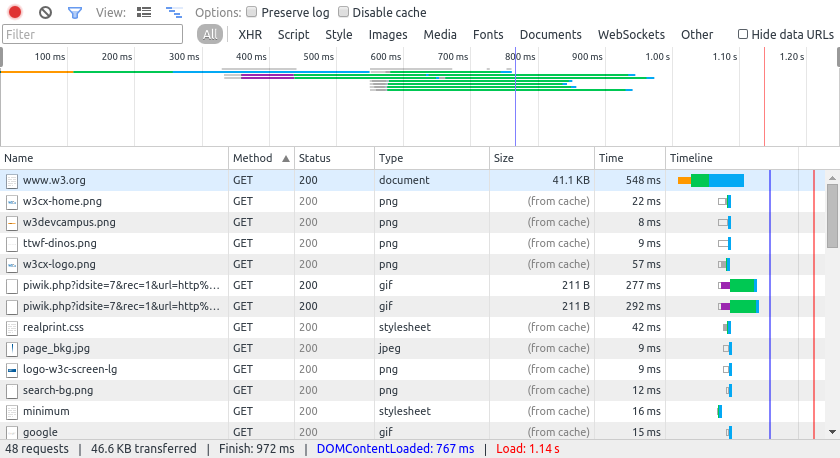
\includegraphics[width=\linewidth]{http_requests}
	\caption{Google Developer Tools window showing HTTP Requests\label{http_requests}}	
\end{figure}

In the above example only the GET HTTP method is used, because the client only requests data from the server, without
sending any data itself. If the client needs to send data to the server, such as form data, or a file, it would still
initiate the connection (the server cannot make requests, only respond, another consequence of statelessness), using
the POST method. While this approach is suitable for a passive, document-based web, where interaction is limited to
jumping from document to document, the web has quickly evolved into an application-based model, where full UIs take
place in the browser space, requiring data be constantly sent back and forth between client and server, in realtime.
This project is one such application.\\

The only way to do this with standard HTTP is periodic polling, which entails large server and network loads. Some
stopgap solutions exist to minimize this overhead, most relevant of which is the Comet web application model. Comet is
based on the concept of long-polling: effectively ``hanging'' the server response until the requested data is
available, and calling another request once the data is received. This approach  still causes increased server loads
but allows some semblance of real-time data transmission. The possibility to use only one connection, as seen in the
previous example was another improvement that became standard in HTTP 1.1. With the HTTP/2 Standard (published in May
2015), the server is allowed to effectively ``push'' data to clients by queuing up more responses than received
requests. However, none of these modifications and hacks are a complete, elegant solution to the problem, given that
HTTP was never intended to be a real-time protocol.\\

That is why other technologies have taken over this new realm of interactivity, providing much more than the ``big,
virtual documentation system in the sky'' \cite{bernerslee09} envisioned by Berners-Lee more than 25 years ago. Some
of them are key parts of this project, as the following sections describe. Still, HTTP remains the initiator for all
these other technologies to function. As of today, any web page you open, no matter how complex the code served in
javascript or flash or any other plug-in still begins with a simple GET request and response.
\section{HTML} \label{HTML}
HTML (Hypertext Markup Language) is the language in which web pages are written. It was created in 1989 by Tim
Berners-Lee as part of his WorldWideWeb, a set of documents linked between each other on a network using the Internet
protocol. It was initially based on SGML (Standard Generalized Markup Language) a document markup language released in
1986 as an ISO Standard (ISO 8879:1986 -- Information processing -- Text and office systems), which was itself derived
from GML (both an acronym for Generalized Markup Language and for Goldfarb, Mosher, Lorie, the last names of its
developers), developed by IBM in 1969.\\

Markup languages in general existed before digital media and still exist in paper based documentation (blue/red
annotations used by editors because lithography/photography/xerography did not capture these colors, the engineering
code for editing documents red = add, blue = delete, green = comment, and many others). In general, markup is a way to
add information regarding the document's structure, presentation, state of development, comments, author, date,
copyright, etc. in a way that is distinguishable from the content of the document. For digital media, it also needs to
be machine-readable, which simply means that a computer must be able to parse this data to extract information. There
are basically two ways of doing this:
\begin{enumerate}
	\item Procedural Markup: A source text is written with instructions for a processing program (equivalent to a
  compiler) to construct the final document. A good example of this method is \TeX, the typesetting system underlying
  the \LaTeX\ macro language (which is itself a mixture of procedural and declarative markup), used to write this
  document.
	\begin{figure}[ht]
    \subfloat[Procedural Source (\LaTeX)]{{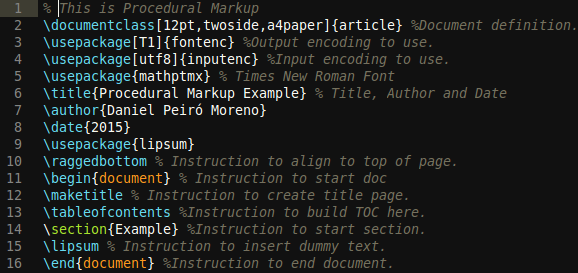
\includegraphics[width=\linewidth/2]{html_procedural_in}}}
    \subfloat[Procedural Output (PDF)]{{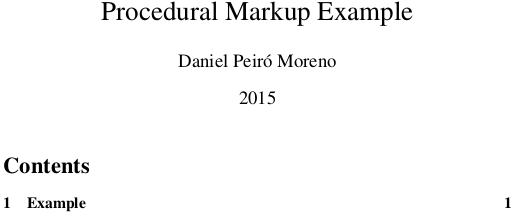
\includegraphics[width=\linewidth/2]{html_procedural_out}}}
    \caption{Procedural Markup Example}
	\end{figure}
	\item Declarative or Descriptive Markup: The content of the text is labeled or ``tagged'' with the markup, without
  giving any instructions on how to process these labels. HTML (especially before HTML5) and XML are clear examples of
  this method.
	\begin{figure}[ht]
    \subfloat[Declarative Input (HTML5)]{{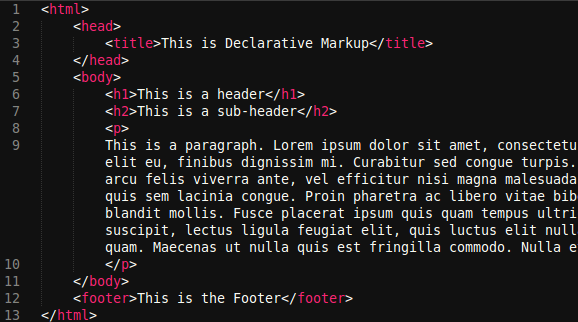
\includegraphics[width=\linewidth/2]{html_declarative_in}}}
    \subfloat[Declarative Output (Google Chrome)]{{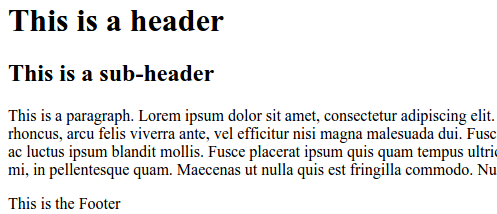
\includegraphics[width=\linewidth/2]{html_declarative_out}}}
    \caption{Declarative Markup Example}
	\end{figure}
\end{enumerate}
HTML and its precursor SGML are essentially declarative markup languages. The main advantage of declarative markup,
and more generally the declarative programming paradigm is the decoupling of the intended result and the processing
required to achieve it. This has been crucial for HTML to be able to evolve and adapt dynamically over decades of
technological innovation. The computers and programs used in 1989 have very little in common with those used today in
many cases. A markup language designed to be ubiquitous, read on an ever changing array of software and hardware
platforms and permanently backwards compatible, where a web page designed in 1991 is just as valid as one designed
using the last specification, has to be as procedurally oblivious as possible.\\

The basic HTML markup unit is the tag. A tag is simply a keyword surrounded by brackets. HTML tags usually come in
pairs, an opening tag and a closing tag (designated adding a forward slash after the first bracket), that give markup
information on the enclosed content:
\begin{figure}[h]
\centering
\RecustomVerbatimEnvironment{Verbatim}{BVerbatim}{}
\begin{minted}[breaklines,fontsize=\footnotesize]{html}
<!--This is a comment-->
<h1>This is a heading</h1>
<p>This is a paragraph</p>
<div>This is a section</div>
<table>
  <tr>
    <th>Table Header Cell 1</th>
    <th>Table Header Cell 2</th> 
  </tr>
  <tr>
    <td>Table Cell 1</td>
    <td>Table Cell 2</td> 
  </tr>
</table>
<ul>
  <li>List Element 1</li>
  <li>List Element 2</li>
  <li>List Element 3</li>
</ul>
<a href="http://www.w3.org">This text links to W3C Web Page</a>
\end{minted}
\caption{Declarative HTML Tags}
\end{figure}\\
All of the tags in the above example are purely declarative. They state what the enclosed text is, leaving it up to
the parser how to obtain the desired result. To extend markup within a tag, attributes are added and given a value. For 
example, the href attribute in the <a> hyper link tag above points to the URL the browser will go to when the text is 
clicked. As the web evolved since it's inception, adding interactivity to documents, more tags were added to HTML that 
weren't so clearly declarative and had a behavioral component, as well as semantic attributes:\\
\begin{figure}[h]
\centering
\RecustomVerbatimEnvironment{Verbatim}{BVerbatim}{}
\begin{minted}[breaklines,fontsize=\footnotesize]{html}
<form action="" method="">
  <input type="text" name="input1"><br>
  <input type="text" name="input2"><br>
  <input type="button" value="value0" onclick="">
  <input type="checkbox" name="input3" value="value1">
  <input type="radio" name="input4" value="value2"><br>
  <input type="radio" name="input5" value="value3">
  <input type="submit" value="Submit">
</form>
\end{minted}
\caption{Behavioral HTML Tags}
\end{figure}\\
These behavioral tags (and many others) were a response to the demand for a more interactive web, not only composed of
linked documents, but of applications implementing business logic and data transactions. They were added by web
browser developers independently, and in consequence were incompatible with other software as well as poorly
documented. In 1994, Tim Berners-Lee created the W3C (World Wide Web Consortium) to solve this problem, attempting to
achieve consensus between browser developers developing standard versions of HTML. This helped HTML remain relatively
simple and consistently usable across browsers. The W3C also attempted to standardize the way browsers parsed HTML,
which initially was very lenient to errors. The repercussions of these attempts will be discussed in section
\ref{HTML5}, specifically related to HTML5, as they indirectly led to the standard.\\

HTML tags can be nested, with the outer tags being called parent tags, and tags enclosed by others called children.
This nested structure, which can also be seen as a tree structure is called the Document Object Model or DOM for short.
This model represents all of the objects included in the document in nodes, with parent nodes encapsulating child nodes,
and one root node that encapsulates all of them. To create the DOM, different browsers use different methods, called
layout engines that parse the HTML to create the DOM Tree. This tree serves only the purpose of correctly representing
nested content on a page, where static web pages are concerned. However, the DOM is crucial for dynamic web pages, as it
provides external controllers, such as JavaScript a model to interact with (see section \ref{JavaScript} on JavaScript).\\

In this project there is just one HTML document (albeit one composed of more than 500 lines of markup) and therefore only
one DOM Tree, as it implements the ``Single Page Application'' user interface paradigm as a means to make the user
experience more fluid and similar to that of a native program. The structure of the page, which is decidedly non-
declarative as a whole, is nonetheless defined using almost exclusively declarative tags. Only multimedia is truly
generated dynamically on the page, with everything else being declared statically, with the caveat of being bi-
directionally bound to a model which in turn is dynamically changed (see section \ref{AngularJS} on AngularJS).\\

The declarative markup method has many advantages as shown: simplicity, portability, light-weight parsing... But it's
main flaw remains that it lacks the ability to create complex structures, interactive structures, and dynamic
structures. Declarative markup is distinctly static in nature: once parsed, the content is presented and remains the
way it was declared (at least in purely declarative tags). This is not a flaw inherent to its design, as it was designed
to markup documents, but one created through the evolution of the web. HTML as a language has itself evolved, blurring
the lines of declarative and behavioral markup (see section \ref{HTML5} on HTML5 for more), but for interactivity and
complexity to truly flourish, markup as a whole just isn't enough. As early as 1995, it became evident that the web
needed a programming language. That language was JavaScript.
\section{JavaScript} \label{JavaScript}
\begin{figure}[h]
\centering
\includesvg[width=1.1\linewidth/4]{./img/javascript}
\caption{JavaScript Badge}
\end{figure}
JavaScript is a programming language. The most common use for JavaScript is running scripts alongside web pages, making
them dynamic and interactive in ways HTML alone cannot. JavaScript was created by Netscape, an early web browser vendor
and developer in 1994, as part of its Netscape Navigator browser. Originally named Mocha, then LiveScript and finally
JavaScript (not because it is related to the Sun developed language, but as an attempt by its creators to use the
popularity of Java for marketing reasons). It was initially conceived as a ``glue'' programming language to be used by
web designers with little programming knowledge or experience to include Java (considered a more ``serious'' and powerful
language at the time) applets in their pages without necessarily knowing anything about Java programming. It quickly
evolved beyond that, becoming a programming language in it's own right. After Microsoft included it in Internet Explorer
3.0 in 1996 (as JScript, to add to the naming confusion), Netscape sought to standardize the language through the ECMA
standards organization, eventually leading to ECMAScript, the current technical name of the language (used only in
standard versions). The current standard is ECMAScript 5 originally released in 2009, while ECMAScript 6 will be released
sometime in 2015. Although JavaScript is mainly used client-side even today, it was originally conceived to also run
server-side. This concept was widely ignored during the early days of the web, focusing on client-side dynamic scripting,
while using other languages (PHP, CGI, Perl, etc.) on the server-side. The late 2000s and early 2010s have seen a
resurgence of the idea of server-side JavaScript allowing full-stack (front-end to back-end in JavaScript) applications,
like this project, to exist. This will be covered in section \ref{TheMEANStack} on the MEAN Stack.\\

The formal classification and description of JavaScript as a language is beyond the scope of this overview, so it won't
be discussed here. Suffice it to say that it's a prototype-based, dynamically-typed scripting language, which allows it
to implement multiple programming paradigms (imperative, functional and object oriented), sacrificing performance (as do
all dynamic languages) and formal elegance for a high level of abstraction, flexibility and dynamic execution.\\

The key aspect of client-side JavaScript is that runs in the browser, dynamically modifying the HTML document. A
JavaScript script is included in an HTML document simply by using the script tag:
\begin{figure}[h]
\centering
\RecustomVerbatimEnvironment{Verbatim}{BVerbatim}{}
\begin{minted}{html}
<script type="text/javascript" src="examplescript.js"></script>
\end{minted}
\end{figure}

As seen in section \ref{HTTP} on HTTP, this tag will trigger a HTTP GET request to the server for the text file
``examplescript.js'', that the browser will parse as JavaScript, and dynamically execute, with total transparency
from the users point of view. This script could, in a typical early web use-case, modify the web page dynamically,
without necessarily triggering new HTTP requests to the server, given that once the script is served, it is running
independently on the client system. For modifications to be possible, a machine-readable model of the web pages' content
and markup is required. The DOM (Document Object Model, see section \ref{HTML} on HTML) is the convention used to model
the page, and is kept in memory by the JavaScript Engine as the global ``state'' of the page. Scripts can then get
information from the model, as well as control and modify the model. The browser will then refresh the representation of
the page, following a classic Model (DOM), View (Browser window), Controller (JavaScript scripts) paradigm.\\

This use-case, while still the most extended use for JavaScript has given way in the last decade and a half to a much
more behavior-centric use, where JavaScript no longer is an add-on or enhancement to HTML, as much as a fundamental part
of how we understand web pages, to the point where the latest standard in HTML includes many tags that are simply useless
without JavaScript to provide the behavior behind them. This demand for interactivity has also led to some pages that are
sloppy when it comes to separating behavior and structure of a web application, tending to use JavaScript for everything,
even when HTMLs declarative approach is more appropriate for a given use-case, simply because JavaScript is more
``comfortable'' from a programmers perspective. This brings with it code maintainability, elegance and performance issues
if not handled correctly. To help maintain declarative and behavioral code separate, and use each one when appropriate,
JavaScript frameworks such as AngularJS have appeared, allowing highly dynamic, complex, single-page web applications to
keep a Model-View-Controller paradigm. This framework, as part of the MEAN Stack, is used in this project (see section
\ref{AngularJS} on AngularJS).

JavaScript essentially provides behavior, interactivity and dynamism to otherwise static HTML. Other methods of adding
these traits to web pages exist and some remain popular today. Java Applets run in a JVM (Java Virtual Machine) once
executed from an HTML document. Adobe Flash (previously Macromedia Shockwave Flash) allows full animations, video and
audio to play embedded inside of a web page. Microsoft Silverlight (now deprecated) served a similar purpose as Flash.
All of these technologies had the major flaw of not integrating with HTML as much as substituting it, or embedding a
``black-box'' in it. This impacts platform compatibility, performance, and accessibility (without going in to the
problems that arise from proprietary technologies). Of the previous, only Flash remains relevant today, mainly as a means
to provide multimedia content, where the HTML standard is considerably lagging behind. But even then, Flash today is
either incompatible or unsupported on all major mobile platforms, and is quickly being substituted with HTML5 by
multimedia providers (Youtube, for example, now defaults to an HTML5 player as opposed to Flash). JavaScript on the other
hand has been consistently relevant since it's inception and continues to grow in importance as a web technology,
expanding to the back-end, and becoming inextricably embedded in the latest HTML standards. This is precisely because it
doesn't try to substitute or deprecate HTML, but complements it by adding behavior to structure, while allowing both to
remain separate.
\section{CSS} \label{CSS}
\begin{figure}[h]
\centering
\includesvg[width=\linewidth/4]{./img/css3}
\caption{CSS3 Badge}
\end{figure}
HTML provides structure to web documents. JavaScript adds behavior, turning documents into applications. CSS (Cascading
Style Sheets) adds style, giving the document renderer instructions on the presentation of the structure created with HTML.
This gives documents and applications, which have no inherent visual representation, a distinct style, as chosen by the
designer, not by the renderer. CSS was created by Håkon Wium Lie and Bert Bos in 1994. It was originally named Cascading
HTML Style Sheets (CHSS), as it was aimed exclusively at HTML styling. The H was soon dropped from the name, as the authors
wanted CSS to be applicable to other markup languages. CSS, like HTML wasn't the first language of it's kind. Style sheet
languages like DSSSL (Document Style Semantics and Specification Language) or FOSI (Formatted Output Specification
Instance) were created for HTMLs precursor, SGML (see section \ref{HTML}). However, these languages didn't allow for style
sheets to be separated from the document, and were therefore unsuitable for the nature of the web, while also being deemed
too complex. CSS has been standardized by the W3C since it's creation, producing three main recommendations:
CSS1 in 1996, CSS2 in 1998, and CSS3 which was divided into modules for different aspects of the language, some of which
have already been finished in the last few years, others still evolving. CSS4 development has begun on completed modules,
but will not be extensively worked on until CSS3 is finalized.\\

Before CSS, HTML either was devoid of any presentational specifications (leaving all styling to the default specified by
the renderer, making all web pages quite simple and unappealing) or had to be styled from within HTML. This was done using
presentational tags, which remained part of HTML standard until HTML4 (see figure \ref{presentational_tags}).\\
\begin{figure}[h]
\centering
\RecustomVerbatimEnvironment{Verbatim}{BVerbatim}{}
\begin{minted}{html}
<h1>
  <font size="3" color="red">This is a heading</font>
</h1>
<body background="bgimage.jpg"><!--Use image as background-->
<strike>This text is strikethrough.</strike>
<img src="exampleimage.png" border="5"><!--Image with 5px border-->
<center>This text will be center-aligned.</center>
</body>
\end{minted}
\caption{Deprecated Presentational Tags \label{presentational_tags}}
\end{figure}

This presented the problem of mixing declarative, structural markup with styling, making the structure much less clear to
the editor, which in turn led to error-prone design, while still being a limited solution, since the amount of tags needed
to be kept in check, if there was to be any structure to the language.\\

CSS allows, similarly to how JavaScript does with behavioral components, the addition of style without substituting
structure while keeping a separate environment for each. With CSS, the only tag necessary is the script tag, or if included
from another file, the link tag:
\begin{figure}[h]
\centering
\RecustomVerbatimEnvironment{Verbatim}{BVerbatim}{}
\begin{minted}{html}
<head>
<link rel="stylesheet" type="text/css" href="stylesheet.css">
</head>

<!--OR-->

<style>
h1 {
font-size: 3px;
color:red;
}
</style>
\end{minted}
\caption{Linking or including CSS in HTML}
\end{figure}
This separates the structure and the presentation of the web page neatly, allowing both to remain clear, readable and
maintainable.\\

The main styling unit of CSS is the rule. A rule is composed of selector and a declaration block. A selector specifies the
target of a set of style specifications (declarations) that follow in the declaration block. In the previous example, there
is only one rule, with selector h1 and declarations font-size and color. This rule will target all h1 tags present in the
document and apply the declarations inside the declaration block to the content of the tag. There are a wide range of
selectors available, from the simplest like the wild-card, *, that targets all elements, to complex, composite selectors
that target elements with certain attribute values (particularly useful is the ".class" selector that targets all elements
with a certain class attribute value), pseudo-selectors that target elements under certain circumstances (``:hover''
targets elements with the mouse over them), etc. which allow complete control over the presentation of web pages.\\

While rules provide granular presentational control over the web page, as a standalone, they would be cumbersome at best
and impossible to implement at worst were it not for cascading. Cascading allows the definition of a hierarchical structure
in the way rules are applied, where rules with a higher priority overwrites lower priority rules. There are several
priority definitions (for example, in line style tags prevail over included stylesheets), but the most important is
selector specificity. If an element fits the target for two or more selectors, the one with the highest specificity will
prevail, if that rule defines a conflicting declaration. For example:
\begin{figure}[h]
\centering
\RecustomVerbatimEnvironment{Verbatim}{BVerbatim}{}
\begin{minted}{css}
/* Applies to all elements */
* {
  color: green;
  text-align: center;
}

/*
  Applies to h1 elements.
  Overrides color from *,
  keeping text-align: center.
*/
h1 {
font-size: 3px;
color:red;
}

/*
  Applies to p elements nested in div elements.
  Overrides both * declarations.
*/
div > p {
  color: blue;
  text-align: right;
}

/*
  All other elements will apply *,
  without need for more rules.
*/
\end{minted}
\caption{Cascading CSS Specificity.}
\end{figure}
\\(Note: Use of * selector is somewhat inefficient and inelegant, used here for illustration purposes).\\

Without this feature, it would be necessary to specify styles for each type of element, or leave some up to the renderer.
This, as previously stated would be tedious for document based pages, and near impossible for applications.\\

This project implements the ``Single Page Application'' user interface pattern, and therefore only one style sheet is used.
In websites with multiple web pages, there's normally one root style sheet that defines the general presentation of the
site, common to all pages, and each page may have it's own particular style sheet for more specific presentation
specification. This allows for neat compartmentalization of styling, which benefits maintainability, future development and
documentation.\\

Some of the more modern modules of CSS3 used in this project (media queries and transitions) will be discussed in section
\ref{HTML5} on HTML5. Even though CSS3 is technically a separate entity and W3C standard, it is most certainly part of the
wider definition of HTML5 as "the cornerstone for modern web applications"\cite{w3c11}.
\section{HTML5} \label{HTML5}
\begin{figure}[h]
\centering
\includesvg[width=1.4\linewidth/4]{./img/html5}
\caption{HTML5 Badge}
\end{figure}
HTML5 is the latest version of the HTML (see \ref{HTML} on HTML in general) Specification Recommendation developed and
published by the W3C (in its final form, development started outside the Consortium) released the 28th of October, 2014.
The significance of this date is somewhat diminished given that HTML5 has been in development since 2004, and many of the
APIs (Application Programming Interface) it specifies have been implemented in browsers preceding the formal release date,
in many cases years in advance.\\

The fundamental change between HTML5 and previous versions of HTML is the shift to a Web Application model from the
original Web Document model. This change came as a response to the direction the W3C had taken after the publication of
HTML 4.0 in 1997, which was much more conservative. At that time, the W3C was very concerned with broken HTML: it is
assumed (including by the W3C\cite{w3cwebquality02}) that 99\% of web pages are not valid HTML. This is made possible by
the lenient error handling methods used by browser HTML parsers. When a browser finds an error in an HTML document 
(incorrect tag spelling, unclosed tags, missing brackets, incorrect nesting order etc.), instead of stopping and not 
rendering the page, it works around the error, displaying the page as well as it can. This allows for web pages to have 
minor errors that do not alter the overall display of the page, remaining usable for most users, and more importantly, 
allowing anybody that has a basic knowledge of the language to write a web page without having to become an expert, 
effectively making HTML a much more accessible and universal language. The downside to this is inconsistency, which is 
what concerned the W3C: What methods are used in this lenient error handling? Are they to be standard? Proprietary? Which 
errors are permissible? Are future browsers going to be able to read invalid pages which were parsed with undocumented 
error handling methods? All these valid concerns lead the W3C to a drastic decision: draconian error handling.\\


The W3C established that the next HTML standard, called XHTML 1.0, would have to be well-formed XML (eXstensible Markup
Language, a profile of SGML) to be rendered. This, technicalities aside, meant that all documents that wanted to be valid
markup under the new specification, would need to have no errors for browsers to render them. If not, the page would not
render and an error message would be presented to the user. Even for a single mistyped tag. This also rendered all
previous, error laden web pages obsolete in the eyes of the W3C.\\

As discussed in previous sections, attempts to deprecate existing HTML or substitute it with something new, have been in
general unsuccessful. XHTML was no exception. Given that the benefits of upgrading were few, and barely apparent for the
general public, web creators didn't make the jump from HTML 4.0. XHTML 1.0 allowed, through a transitional loophole, the
possibility of declaring the document as XHTML while keeping lenient error handling from HTML 4.0. Even then, adoption was
slow, but when XHTML 1.1 closed this loophole, it sealed its fate as a failed ``upgrade''.\\

After XHTML, the W3C was at an impasse of sorts. It had spent years on the development of XHTML, which had a very low
adoption rate and the power of home computing was sky rocketing, leading to demands for web applications instead of
documents to increase immensely. In 2004, it held a workshop (The W3C Workshop on Web Applications and Compound Documents
\cite{w3c04}) to define the future of web applications. Many manufacturers and interest groups proposed that a series of
mid-level APIs should be developed as extensions to HTML and CSS for use in Web Applications as opposed to fully fledged OS
-Level APIs. This meant leaning toward in-browser solutions as opposed to ``black-box'' plug-in software (such as Java
Applets or Flash). This proposal was rejected (see Workshop Summary straw poll topic no. 3 in \cite{w3c04}), and led to a
group of the proposers to create a work group outside the W3C, the WHAT Working Group (Web Hypertext Applications
Technology Working Group). This group went in the opposite direction the W3C did to solve HTMLs error handling problems
and the evolution of the web. Instead of dropping error handling altogether, like XHTML did, the WHAT group decided it
would specify and document the way lenient error handling works, so that it would no longer rely on proprietary, poorly
documented solutions that made future proofing and maintaining compatibility among different browsers virtually
impossible. This wasn't as easy as the XHTML solution, in fact it took 5 years to complete, but it allowed full backwards
compatibility for older pages, a crucial aspect of evolving the web, as seen in previous sections. For Web Applications,
the WHAT group turned away from plug-ins, and started work on three of the most important multimedia APIs present in
HTML5: Canvas (direct-mode drawing) and native Audio/Video support.\\

In 2006, Tim Berners-Lee announced that the W3C would start working with the WHAT WG to evolve the web. The new HTML
Specification that would come from this new group, would be called HTML5.\\

HTML5 introduced a long list of new features to HTML, most of them directed at Web Application Development:
\begin{itemize}
  \item \textbf{Canvas Element}: Direct Mode 2D Drawing. Essentially allowing for fully native animations.
  \item \textbf{Audio and Video Element}: Native multimedia support, effectively deprecating flash.
  \item \textbf{Geolocation}: Allows sharing the clients location with the application seamlessly.
  \item \textbf{Local Storage}: Allows the application to store data on the clients computer.
  \item \textbf{Offline Web Applications}: Once downloaded, the application can run without being connected to the Internet.
  \item \textbf{WebSockets}: Full duplex communication between client and server, in one TCP connection. (Now a separate specification)
  \item \textbf{Web Workers}: JavaScript running in the background, taking full advantage of the client CPUs power for heavy tasks.
\end{itemize}
While others were much needed upgrades and deprecations of HTML 4.0 features, such as the addition of a wealth of new
controls to forms and semantic tags, as well as the removal of presentational tags altogether. Only the features used in
this project will be discussed briefly further.
\subsection{HTML5 Semantics}
\begin{figure}[h]
\centering
\includesvg[width=1.4\linewidth/8]{./img/html5_semantics}
\caption{HTML5 Semantics Badge}
\end{figure}
HTML5 Semantics are used to more clearly and succinctly define the elements content. This improves the readability of the
markup and allows browsers to make better accessibility tools. It makes the markup easier to read by eliminating
unnecessary text:\\

\begin{figure}[h]
\centering
\RecustomVerbatimEnvironment{Verbatim}{BVerbatim}{}
\begin{minted}{html}
<!--In XHTML 1.0-->
<!DOCTYPE html
          PUBLIC "-//W3C//DTD XHTML 1.0 Strict//EN"
          "http://www.w3.org/TR/xhtml1/DTD/xhtml1-strict.dtd">
<html xmlns="http://www.w3.org/1999/xhtml"
      lang="en"
      xml:lang="en">
</html>
<!--In HTML5-->
<!DOCTYPE html>
<html></html>
\end{minted}
\caption{HTML5 Semantics: Text Usage Comparison}
\end{figure}
And by giving names to typical web page components:\\

\begin{figure}[h]
\begin{center}
  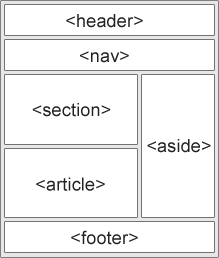
\includegraphics[width=\linewidth/3]{html5_layout}
  \end{center}
  \caption{HTML5 Semantics: Typical Page Layout. Source: \href{http://www.w3schools.com/html/html5_semantic_elements.asp}{
  W3Schools}.}
\end{figure}
This allows web browsers to better understand what the content is declared as, and choose to present it in different ways (
for example, a page with an article and a header might be presented differently on a mobile browser to enhance the reading 
experience), and allows for accessibility features such as text-to-speech to present the content in a fitting manner.\\

In this project, the page is written using HTML5 semantics, reducing the amount of superfluous text, making it easier to
read (taking into account the complexity of the liquid layout). It also uses the header and footer tags to frame the
controls, using the header as the title of the page, and the footer to include copyright acknowledgments and references.
\begin{figure}[h]
\begin{center}
  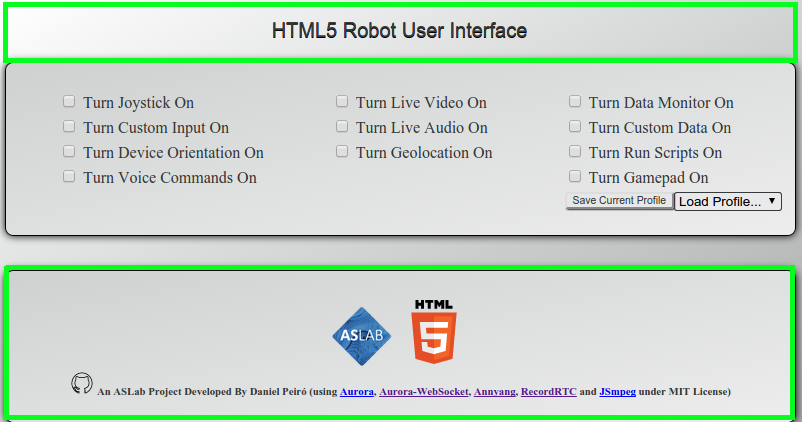
\includegraphics[width=\linewidth]{html5_headerfooter}
  \end{center}
  \caption{HTML5 Semantics: Use of Header and Footer (Marked in green) in HRUI}
\end{figure}
\subsection{HTML5 Canvas Element} \label{html5canvaselement}
\begin{figure}[h]
\centering
\includesvg[width=1.4\linewidth/8]{./img/html5_canvas}
\caption{HTML5 Graphics Badge}
\end{figure}
The Canvas element is, in the simplest terms possible, a rectangle in a web page in which a JavaScript script can draw
anything. It allows things as simple as drawing a line with the cursor, to full fledged game graphics, and requires
nothing but a canvas element (\mintinline{html}{<canvas></canvas>}) and access from JavaScript to said element. By
changing the drawing at a fast enough frequency, animation becomes trivial.\\

In this project, the canvas element is used for three of its modules. It's used to create virtual joysticks for the user
to control dynamically with the mouse or using a touch interface (see section \ref{joystick} on the Joystick input module).\\

\begin{figure}[h]
\begin{center}
  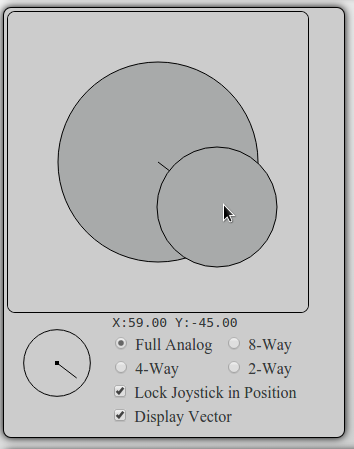
\includegraphics[width=\linewidth/3]{joystick}
  \end{center}
  \caption{HTML5 Canvas: Joystick in HRUI. (2 Canvas Elements: Joystick and Vector)}
\end{figure}
It's used for the live video feed, using JSMpeg, a MPEG1 decoder written in JavaScript (see section \ref{livevideo} on the
Live Video module). It's also used for the dynamic obstacle map in the data monitor module (see section \ref{datamonitor}),
which can be generated from the server, uploaded by the user or can even be drawn on the fly with the cursor or touch
interfaces (see figure \ref{html5_map}).\\

\begin{figure}[h]
\begin{center}
  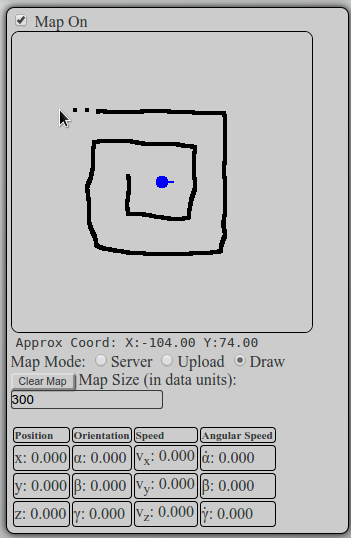
\includegraphics[width=\linewidth/3]{html5_map}
  \end{center}
  \caption{HTML5 Canvas: Map in HRUI. (Black: Drawn Obstacles. Blue: Robot Pos.)\label{html5_map}}
\end{figure}
The Canvas API allows for essentially any sort of content to appear on a website natively without the need for flash, which
was the go-to resource for animation previously. This amounts to a big leap in graphics and animation versatility for HTML.\\

\subsection{HTML5 WebSockets} \label{html5websockets}
\begin{figure}[h]
\centering
\includesvg[width=1.4\linewidth/8]{./img/html5_connectivity}
\caption{HTML5 Connectivity Badge}
\end{figure}
WebSockets allow for full-duplex communication between server and client using one TCP connection. As its name implies it's
most easily described as an implementation of TCP/IP Sockets for the web. It allows for fully bidirectional communication,
using only one HTTP request (see section \ref{HTTP} on HTTP), that is upgraded to a WebSocket connection. This HTTP handshake
is important, as it allows for a graceful backwards compatibility, using the same technology as standard web pages.\\

WebSockets are essential for this project. As a real-time application, data needs to move to and from the client and the
server constantly to relay instructions from the controls to the back-end, and update output data to the front-end.
Furthermore, to live stream media from the server to clients, WebSockets are used, providing minimal latency. Without
WebSockets this project would be almost impossible to achieve, with any measure of success.\\

The WebSockets API in HRUI is implemented in two forms: raw and through the Socket.IO framework. The raw form creates and uses
WebSockets through direct calls to the API and is used for media streaming. The Socket.IO framework adds a layer of
abstraction to WebSockets, by creating an event-based model. An event is a message that is broadcast by an emitter and
captured by a listener. The emitter and listener are the server and client, and vice versa. An event carries attached to it a
JavaScript object which will be received by the listener. The programmer creates these asynchronous events on either the
server or the client, establishing the behavior of the listener. For example: Every 50 ms the back-end wants to send the front-
end an update on the value of X in the robots position. With Socket.IO (after setup) the code would be:\\

\begin{figure}[h]
\centering
\RecustomVerbatimEnvironment{Verbatim}{BVerbatim}{}
\begin{minted}[fontsize=\footnotesize]{javascript}
//On the Server side:
//[...](setup and surrounding code omitted for clarity)
var x = 10; //value of robot X coordinate (defined here for brevity)

socket.emit("UPDATE_X", x);
//emit an event with message UPDATE_X and data x (value: 10)

//On the Client side:
//[...](setup and surrounding code omitted for clarity)
socket.on("UPDATE_X", function(received_x) {
              console.log(received_x);
            };
//listen for an event with message UPDATE_X
//and print the value of the data received to the console.
\end{minted}
\caption{HTML5 WebSockets: Socket.IO Event Example}
\end{figure}
This added layer of abstraction makes using WebSockets very simple, needing only to define when and where in the code events
are generated and adding listeners for these events. It also makes code much easier to understand, and much more structured,
closer to the business logic and separated from low level serializing and underlying connections.
\subsection{HTML5 Device Access}
\begin{figure}[h]
\centering
\includesvg[width=1.4\linewidth/8]{./img/html5_device_access}
\caption{HTML5 Device Access Badge}
\end{figure}
HTML5 Device Access allows the web application to use the hardware of the machine the browser is running on. This means
anything from microphones and cameras to accelerometers and GPS data.\\

HRUI makes full use of three of these APIs:\\

\begin{itemize}
  \item \textbf{Microphone}: The Voice Command module (see section \ref{voicecommands}) uses device access to receive audio
  from the users microphone, which is then recognized (using Annyang) into commands which are sent to the server for use (see
  figure \ref{html5_voice}). It also uses the WebRTC API to enable an alternative in non-chromium browsers that don't have the
  speech recognition API, by recording a 5 second audio clip that is sent as a .wav file to the server. WebRTC started out as
  part of HTML5 but has spun out into its own specification, that allows for peer-to-peer server-less audio and video sharing,
  among many other multimedia uses which are outside of this reports scope, since they're not used in this project.

  \begin{figure}[h]
    \begin{center}
      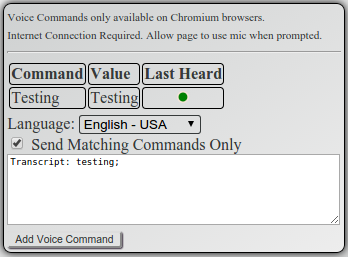
\includegraphics[width=\linewidth/2]{html5_voice}
    \end{center}
    \caption{HTML5 Device Access: Voice Commands in HRUI.\label{html5_voice}}
  \end{figure}
  \item \textbf{Device Orientation}: The Device Orientation module (see section \ref{deviceorientation}) gets the orientation,
   velocity and acceleration from the device (if available) and sends it to the server for use (see figure 

  \ref{html5_orientation})
  \begin{figure}[h]
    \begin{center}
      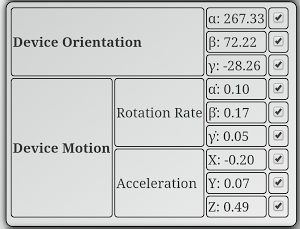
\includegraphics[width=\linewidth/2]{html5_orientation}
    \end{center}
    \caption{HTML5 Device Access: Device Orientation in HRUI.\label{html5_orientation}}
  \end{figure}
  \item \textbf{Gamepad}: The Gamepad module (see section \ref{gamepad}) uses the Gamepad API to get the inputs of a gamepad
  connected to the client machine and send them to the server for use. This extends the HRUI web application controls to
  virtually any device that can be connected to a web capable device as an input, allowing for external hardware to function
  seamlessly with this project with little to no integration effort. However, this API is still experimental at the time of
  writing, and support is limited to a few browsers (Chrome and Firefox mainly), with different implementations that require
  tweaking of parameters (mainly the mapping of buttons, which changes from Chrome to Firefox and with the controller in use)
  for consistent usage.
\end{itemize}
\subsection{HTML5 Styling} \label{html5styling}
\begin{figure}[h]
\centering
\includesvg[width=1.4\linewidth/8]{./img/html5_css3}
\caption{HTML5 Styling Badge}
\end{figure}
HTML5 Styling is actually a misnomer, albeit one used by the W3C, because it considers that HTML5 refers to more than just the
latest HTML Recommendation, encompassing several specifications and should be used as an umbrella term to encapsulate all
technologies of the modern web, calling HTML5 "The cornerstone for modern Web applications"\cite{w3c11}. This is cause of some
debate among enthusiasts, but controversy aside, the fact is that HTML5 has no significant styling features (in consonance
with the separation between declarative and presentational discussed in previous sections), relying on the CSS3 (Cascading
Style Sheets, see section \ref{CSS}) specification for innovation in this aspect.\\

In HRUI many new CSS3 features are used to make the application more visually attractive and useful on different devices:\\

\begin{itemize}
  \item \textbf{Media Queries}: One the most useful additions made to CSS3 is the ability to apply styles to different
  viewports (the space where the web page is rendered in a browser) and device types without having to make different versions
  of the site, by using media queries. A media query basically defines a subset of styling rules that apply only to viewports
  that fit a certain criteria, while keeping in place the cascading nature of CSS. This means that by making, for example, a
  media query on the pixel width of the screen, a set of rules will be applied that can drastically change the presentation of
  the page. In HRUI only one media query is made, specifically to target smartphones (truncated for brevity):\\

  \begin{figure}[h]
    \centering
    \RecustomVerbatimEnvironment{Verbatim}{BVerbatim}{}
    \begin{minted}[fontsize=\footnotesize]{css}
      @media only screen and (max-width: 480px) {
          .frame {
              width: 100%;
          }
          #rightColumn, #centerColumn, #leftColumn {
              float: left;
              clear: both;
              width: 98%;
          }
      }
    \end{minted}
    \caption{HTML5 Styling (CSS3): Media Query in HRUI}
  \end{figure}
  Which targets screens under 480 pixels wide and applies the enclosed rules only to those screens. All other styling is
  maintained and applied, through cascading. These rule (and others omitted for brevity) make all modules occupy the whole
  width of the screen, more appropriate for small, touch based devices than the three-column default for computers and
  tablets. The user can then scroll through the modules to use them since including more than one module on a smartphone
  screen at once would clutter the interface and make it virtually unusable. This approach makes a necessary compromise by
  allowing the active visualization of one module at a time, while allowing all modules to run in the background, visible at
  the slide of a finger.
  \begin{figure}[h]
  \captionsetup{justification=centering}
      \begin{center}
        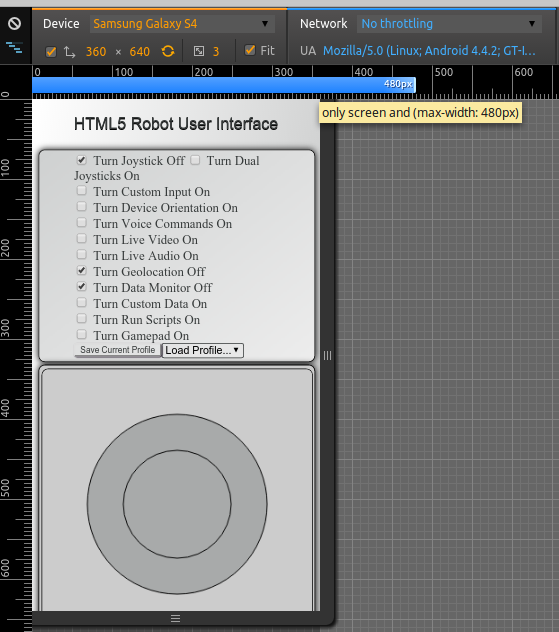
\includegraphics[width=\linewidth/3]{html5_css_mq2}
      \end{center}
      \caption{HTML5 Styling (CSS3): HRUI Smartphone version\\(simulated SGS4 using Chrome Dev Tools. Blue bar marks the
      detected media query)}
  \end{figure}
  \begin{figure}[h]
    \begin{center}
      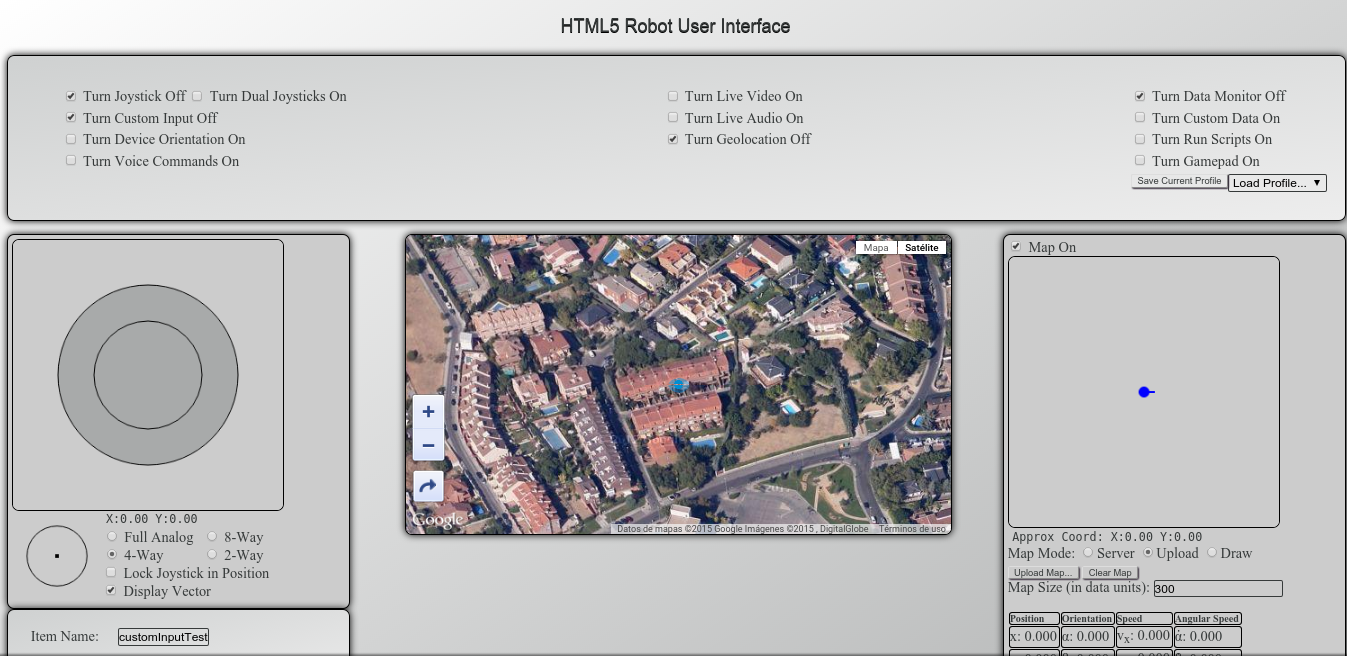
\includegraphics[width=\linewidth/2]{html5_css_mq1}
    \end{center}
    \caption{HTML5 Styling (CSS3): HRUI Laptop version}
  \end{figure}
  \item \textbf{Transitions}: CSS3 Transitions can make the value of element properties change over time, creating an
  attractive visual effect. HRUI uses this feature (combined with AngularJS Animate, see section \ref{AngularJS}) to animate
  module activation and deactivation with a fade in/out effect. Because this specification is still not final, it's still
  necessary to include vendor prefixes to transition rules, as each one implements the feature in slightly different ways.
  \begin{figure}[h]
    \centering
    \RecustomVerbatimEnvironment{Verbatim}{BVerbatim}{}
    \begin{minted}[fontsize=\footnotesize]{css}
    -webkit-transition: all 0.7s ease-in-out;
    -moz-transition: all 0.7s ease-in-out;
    -ms-transition: all 0.7s ease-in-out;
    -o-transition: all 0.7s ease-in-out;
    transition: all 0.7s ease-in-out;
    \end{minted}
    \caption{HTML5 Styling (CSS3): Transitions in HRUI.}
  \end{figure}
  \item \textbf{Gradients}: CSS3 Gradients make backgrounds change from one color to another across the surface of the
  element. It's used in HRUI to provide a smooth silver background with a lighting effect. As with CSS3 Transitions, vendor
  prefixes are required.
  \begin{figure}[h]
    \centering
    \RecustomVerbatimEnvironment{Verbatim}{BVerbatim}{}
    \begin{minted}[fontsize=\footnotesize]{css}
    background-image: -webkit-gradient( linear, left top, right bottom,...);
    background-image: -o-linear-gradient(right bottom, #CFD1D1 0%, #EDEDED 100%);
    background-image: -moz-linear-gradient(right bottom, #CFD1D1 0%, #EDEDED 100%);
    background-image: -webkit-linear-gradient(right bottom, #CFD1D1 0%, #EDEDED 100%);
    background-image: -ms-linear-gradient(right bottom, #CFD1D1 0%, #EDEDED 100%);
    background-image: linear-gradient(to right bottom, #CFD1D1 0%, #EDEDED 100%);
    \end{minted}
    \caption{HTML5 Styling (CSS3): Gradients in HRUI.}
  \end{figure}
  \begin{figure}[h]
    \begin{center}
      \frame{
\includegraphics[width=\linewidth]{html5_css_gradient}}
    \end{center}
    \caption{HTML5 Styling (CSS3): HRUI Header Gradient}
  \end{figure}
  \item \textbf{Pseudo Classes}: CSS3 Pseudo Classes are classes that target elements that match a given criteria. For example
  the :hover pseudo class targets elements over which the cursor is currently held. This allows for some dynamic style changes
  following user actions. Pseudo Classes existed in CSS2, but CSS3 added 16 new ones, including the one used in HRUI to change
  the color of disabled buttons to show the situation to the user.
  \begin{figure}[h]
    \centering
    \RecustomVerbatimEnvironment{Verbatim}{BVerbatim}{}
    \begin{minted}[fontsize=\footnotesize]{css}
    button:disabled {
    color: grey;
    box-shadow: inset 1px 1px 1px #3D3242;
    }
    \end{minted}
    \caption{HTML5 Styling (CSS3): Pseudo Classes in HRUI.}
  \end{figure}
  \item \textbf{Rounded Borders \& Box Shadows}
  \begin{figure}[H]
    \begin{center}
      \frame{
\includegraphics[width=\linewidth/3]{html5_css_round}}
    \end{center}
    \caption{HTML5 Styling (CSS3): HRUI Rounded Borders and Box Shadow Example}
  \end{figure}
\end{itemize}

HRUIs' single web page is written in valid HTML5. What this means is that it adheres strictly to the W3C Recommendation and
is well-formed (does not contain errors). This has been checked throughout the project using the W3C HTML Validation Service
\cite{w3cvalidation} to fully comply with the specification.
\section{The MEAN Stack} \label{TheMEANStack}
\begin{figure}[H]
    \begin{center}
      
\includegraphics[width=0.7\linewidth]{mean}
    \end{center}
    \caption{MEAN Stack Logo}
  \end{figure}
The MEAN (MongoDB, Express, AngularJS, Node.js) Stack is an open source web development full stack specifically suited for
web applications. To understand the definition, the concept of the software engineering stack must be understood first.\\

A stack in software engineering (not to be confused with the programming concept of the stack, an abstract data collection
used to store and retrieve data in programs using ``push and pop'' instructions) is a collection of software or technologies
used to create a complete solution for the development of an application. This software bundle serves as a platform for the
application, providing the software required to realize its architecture. In web development this architecture is typically a
server-client paradigm (see chapter \ref{systemarchitecture} on the HRUI System Architecture, particularly section 
\ref{clientserverpattern} on the Client-Server pattern), in which the main components traditionally are: an operating system that will
run the server; web server software; a database to store the application data (a web server is stateless, as discussed in section
\ref{HTTP}, so a database is needed to supply "memory" to the architecture); and finally a programming language in which programs or
scripts will be written to perform the tasks required by the application on the server.\\

The most used and famous web development stack is of course the LAMP (Linux OS, Apache Web Server, MySQL Database, PHP
programming language) Stack, and its variants (MAMP for Mac OS, WAMP for Windows OS, LAMP with Python or Perl as programming
languages...). It's been the default way to create a web server since the mid 90s', mainly because of its simplicity and
extensibility, allowing for the last component, the programming language to be virtually any language, by using scripts that
can call external programs. Of course, it's also fully open source, which is also one of its greatest strengths. The biggest
problem with the LAMP stack in modern web application development is that it relies heavily on HTTP requests (see section \ref{HTTP} on
HTTP) and therefore is not suited to real-time constraints. The way a LAMP stack generally functions requires that for every HTTP
request made from the client, either an HTML document is served or a script (PHP/Python/Perl) is run, that then
generates HTML output that is sent back to the client by the server. This last method is called CGI (Common Gateway
Interface), used since the mid 90s' to create more interactive web content circumventing the constraints of a document-based
web, but even this is unsuitable for real-time, as these requests would have to be made every few milliseconds to achieve the
required responsiveness, resulting in unsustainable overhead on the server. The true solution for real-time web applications
is WebSockets (see section \ref{html5websockets} on HTML5 WebSockets) that allow bidirectional communication over one TCP
connection upgraded from an HTTP request. The LAMP Stack was developed much before this technology and is built on a
completely different communication pattern, so trying to integrate WebSockets into LAMP makes little sense when building a new
application. It is possible (using PHP or with mods to the Apache Server itself), but it goes against the paradigm of a LAMP
server, making it inelegant and bound to be a limited solution.\\

The MEAN Stack fully supports WebSockets and in fact is the go-to way of implementing them in modern web applications. The
main reason for this is part of the definition given at the beginning of this section: the MEAN Stack is a \textit{full}
stack. This means that unlike other web development stacks (such as LAMP), the stack provides software for the development of
the front-end (the client-side) as well as the back-end (the server-side). Furthermore, both client and server (front-end and
back-end) are written in the same language: JavaScript. This allows for code on both sides to be nearly identical in their
implementation and makes a protocol like WebSockets that allows for full bidirectional communication very easy to implement
because no translation of the data needs to take place on the application level. Either the client or the server send data
over this protocol in a way the receiving program can instantly comprehend, because it's in the same language, JavaScript  
(see section \ref{html5websockets} for an example). This makes the MEAN Stack the best solution for real-time modern web
applications, such as this project.\\

Another great advantage of the MEAN Stack is its portability. In the acronym, no operating system is included because the MEAN
Stack can run on any OS that can run its components, completely agnostically. This is possible thanks to Node.js, which will
be discussed further in the following section. What this means is that an application using the MEAN Stack can have its
server deployed on Linux, Mac or Windows, or any OS that has Node.js and MongoDB software packages without making any changes
to the code, if no OS level APIs or external programs are used that require a specific platform. In HRUI, media streaming is
restricted to the Linux platform because access to OS level APIs (Unix device files that are only present in Linux
distributions like /dev/videoX) and external programs (FFMpeg/Avconv) is required, but the core application is fully
functional on any platform, without any changes made to the code (media streaming will simply not work, without crashing or
halting the application, using error handling procedures).\\

To complete the breakdown of the definition of the MEAN Stack, open-source software is software that has its source code
available to the public for study, discussion, distribution, modification and redistribution for any purpose. The Open Source
Software Movement is discussed as part of the social and professional implications of engineering in chapter \ref{conclusions}
section \ref{opensourcemovement}.\\

In the following sections, the components of the MEAN Stack will be briefly discussed.\\
\newpage
\subsection{Node.js} \label{nodejs}
\begin{figure}[H]
\centering
\includesvg[width=0.7\linewidth]{./img/nodejs}
\caption{Node.js Logo}
\end{figure}
The creators of Node.js define it as ``a platform built on Chrome's JavaScript runtime for easily building fast, scalable
network applications. Node.js uses an event-driven, non-blocking I/O model that makes it lightweight and efficient, perfect
for data-intensive real-time applications that run across distributed devices''\cite{nodejs15}. This essentially means that
it's a modified version of the JavaScript engine (the software that runs JavaScript in browsers) present in the Google Chrome
Browser (the V8 JavaScript Engine) that runs locally instead of in the browser. The JavaScript code that's usually run
alongside HTML to manipulate the DOM is run locally, independent from the DOM, used as any other general purpose programming
language.\\

Node.js was created by Ryan Dahl in 2009 after feeling frustrated by traditional request-response centric servers that don't
acknowledge concurrent requests (particularly after seeing how a file upload app was inefficiently requesting the server to
update the percentage of uploaded data\cite{nodesummit12}) and constantly lag the user experience waiting for requests to
process synchronously. He decided to create a framework combining JavaScript, a very well known language, the Google Chrome V8
JavaScript engine that was released in 2008 as open source software, and non-blocking IO, for web applications that required
real-time data transmission.

The V8 JavaScript engine on which Node.js is based, is somewhat different to previous JavaScript engines in that it compiles
the code into machine code before execution instead of interpreting it on the fly. Without going into more technical
explanations, this is the same difference between C code that is compiled into machine code that runs directly on the CPU of
the computer, or any interpreted language such as Python that is interpreted instruction by instruction. In short, compiled
code will always be faster than interpreted code. This makes the V8 engine very fast, compared to other interpreting engines.
Another consequence of using an engine like this is that all Node.js applications are cross-platform. Since all the code is
compiled into machine code by the engine, any machine that can run the engine can run any Node.js application, similarly to
how any machine that can run the JVM (Java Virtual Machine) can run any Java program. Of course, if the application makes use
of OS Level APIs or requires external programs, it will be compromised when deployed on different platforms, but any fully
native apps will run indistinguishably on different platforms. In the case of HRUI, which does use external programs and OS
level APIs, error handling functions permit the application to handle other platforms, downgrading the application without
crashing it (media streaming will not work on platforms other than Linux). Node.js is available for most popular Linux
distributions, MAC OSX, Windows and runs on 32/64 bit architectures and ARM.\\

Node.js is event driven, which in short means that it does not run code synchronously, instead relying on listening for events
(any significant change in the state of the application is called an event) that are handled by functions called callbacks.
The main loop of a Node.js app is reduced to listening for events and directing them to the function that handles that particular
event, which in turn should have a callback function that is run when the handler is done. What this means without going into
technical details is that well designed Node.js applications are extremely lightweight when it comes to CPU load, because most
of the time, the application is not doing anything, in contrast with synchronous applications, that are constantly loading the
CPU with instructions because they have to be executed in order. This makes it specially suited for portable applications,
that need to run on low frequency CPUs. This also makes it very well suited for web applications that require a large amount
of concurrent connections all with the same priority. In layman's terms, when a client requires a task performed by the
server, instead of having to execute the task immediately without doing anything else, the task is queued to start, while the
server goes back to listening for more client requests. Once the CPU has gotten around to finalizing the task (scheduling its
CPU time with the rest of concurrent tasks), the callback function is called signaling the completion to the server, which can
then provide the response to the client. This prioritizes the responsiveness towards the clients, as no request is lost or put
on hold because a task is still executing.\\

This makes Node.js ideal for a single-page GUI (Graphical User Interface) web application that requires responsiveness and 
real-timedata transmissions, such as HRUI. With a traditional back-end, it would be near impossible to achieve a responsive
interface to represent data updates on the page and send commands from the client in milliseconds. Synchronous requests would
block concurrent tasks, meaning that, for example, a flick of the joystick would make the reception of position data lag, or
vice versa.\\

Node.js has a vibrant community of developers making modules that are freely available for use through node's package manager,
NPM. Installing new modules for use in a project is as simple as running the command ``npm install package''. HRUI itself can
be installed simply by running ``npm install hrui'' which will install all dependencies automatically and get the latest
version of hrui from github. HRUI uses many of these packages, including but not limited to:
\begin{itemize}
  \item \textbf{Socket.IO}: An event-base framework for WebSockets (see section \ref{html5websockets} for more).
  \item \textbf{Monk}: An abstraction layer to access the MongoDB Node.js driver.
  \item \textbf{PNGJS}: A PNG Image decoder/encoder used to generate the map from a binary-matrix/parse the user-drawn map.
  \item \textbf{Busboy}: A module that parses incoming HTTP requests, used to accept file uploads from the client (map image).
\end{itemize}
The most important module used in HRUI is Express, which is discussed in the following section.
\subsection{Express} \label{express}
\begin{figure}[H]
  \begin{center}
    
\includegraphics[width=0.7\linewidth]{express}
  \end{center}
  \caption{Express Logo}
\end{figure}
Express is a Node.js module defined as a routing and middleware web framework. What this essentially means is that express functions as
a minimal web server, relying on middleware functions to provide responses to HTTP requests (see section \ref{HTTP} on HTTP for more on
requests). Middleware functions are simply handler functions that receive a request through Express, process it in whatever manner
necessary and either provide a response or pass the request onto the next middleware function in line. The following example illustrates
a basic Express server.
\begin{figure}[H]
  \centering
  \captionsetup{justification=centering}
  \RecustomVerbatimEnvironment{Verbatim}{BVerbatim}{}
  \begin{minted}[fontsize=\footnotesize]{javascript}
  var express = require('express'); //Require the express module (equivalent to include in C)
  var app = express(); //Instantiate the express framework 

  //Middleware function: Called on GET Request on the root of the server
  app.get('/', function (req, res) {
    //req contains the HTTP request. This instruction prints it to console.
    console.log(req);
    //res is the HTTP response. This response is just a string confirming reception.
    res.send('Response: Request Received');
  });

  var server = app.listen(3000, function () {
    console.log('Server listening on port 3000.')
  });
  \end{minted}
  \caption{Express minimal web server: Middleware functions.\\(modified from source: \url{http://expressjs.com/})}
\end{figure}
Running this code would print to the console ``Server listening on port 3000.''. Using any web browser and opening the URL
http://localhost:3000 would print the response ``Response: Request Received'' in the browser. With express, it takes less than 10 lines
of code to create a web server. It's important to note that these middleware functions are non-blocking, meaning that they are not
executed synchronously immediately upon request, instead being run asynchronously with the server receiving notification of the response
when the processing is complete. This benefits responsiveness when handling many concurrent requests and is part of the Node.js
non-blocking I/O event driven philosophy (see the previous section \ref{nodejs}). Express allows for all sorts of middleware, not just
request-response functions. Many third-party express middleware is available through npm (Node Package Manager), some of them used in
this project. Middleware used in HRUI:
\begin{itemize}
  \item \textbf{Compression}: this middleware compresses all HTTP responses using gzip reducing the amount of data transmitted, making
  more efficient use of network resources (compression can be confirmed looking at the value of the HTTP header ``Content-Encoding'' or
  using a website like whatsmyip.org).
  \begin{figure}[H]
  \captionsetup{justification=centering}
  \begin{center}
    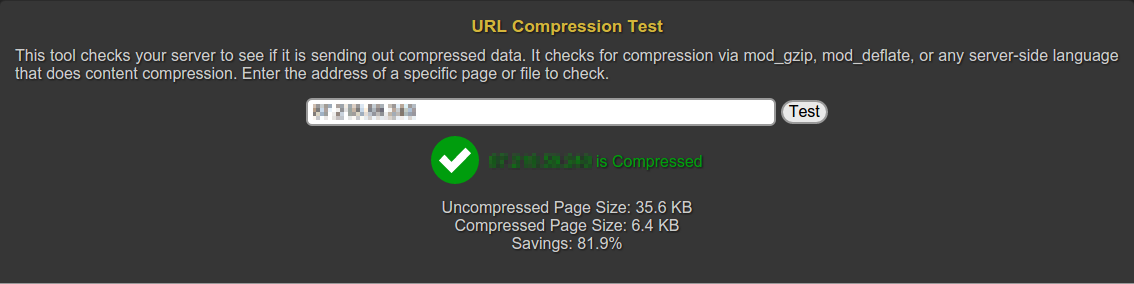
\includegraphics[width=\linewidth]{express_compression}
  \end{center}
  \caption{Express Middleware: Compression. Results of compression test (81.9\%)\\(Source: \url{http://www.whatsmyip.org/})}
  \end{figure}
  \item \textbf{Busboy}: HTTP Request parsing middleware. Parses the HTTP request and allows events to arise on certain types of
  requests like POST requests with files attached. This is used in HRUI to upload a map from the client to the server and save it on the
  server.
  \begin{figure}[H]
  \centering
  \captionsetup{justification=centering}
  \RecustomVerbatimEnvironment{Verbatim}{BVerbatim}{}
  \begin{minted}[fontsize=\footnotesize]{javascript}
  //Setup map upload http response
  var busboy = require('connect-busboy');
  app.use(busboy());
  //a POST request is made to /mapupload with a file attached to it.
  app.post('/mapupload', function(req, res) {
      var fstream;
      req.pipe(req.busboy);
      //event handler when busboy detects a file attachment.
      req.busboy.on('file', function(fieldname, file, filename) {
          //write attached file to disk asynchronously.
          console.log("HRUI: Uploading " + filename + ' to public/images/uploadmap');
          fstream = fs.createWriteStream(__dirname + '/../public/images/uploadmap');
          file.pipe(fstream);
          //once written to disk, respond to client.
          fstream.on('close', function() {
              res.send('Uploaded');
              console.log("HRUI: Uploaded " + filename + ' succesfully');
          });
      });
  });
  \end{minted}
  \caption{Express Middleware: Map Upload with Busboy code (Modified for clarity)}
  \end{figure}
  \item \textbf{Morgan}: Logger middleware. Logs to the console all HTTP requests along with the status and timing of the response.
  \begin{figure}[H]
  \captionsetup{justification=centering}
  \begin{center}
    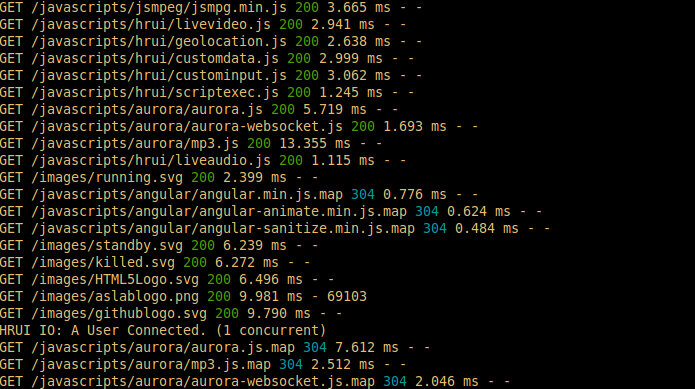
\includegraphics[width=0.7\linewidth]{express_logger}
  \end{center}
  \caption{Express Middleware: HRUI Example Morgan Logger Output\\(Normally configured to only show errors with response code > 400)}
  \end{figure}
  \item \textbf{Express Static}: This first-party middleware makes serving files from a directory as simple as: \mintinline{javascript}{app.use(express.static('public'));} Where 'public' is the folder containing the static content. This is useful in sites with few web
  pages, such as single-page applications like HRUI.
  \item \textbf{Serve Favicon}: Middleware to serve a favicon to web browsers. A Favicon is the icon that appears in modern browsers
  next to the URL in the search bar and in Bookmark bars. HRUI's Favicon is an NES Controller.\includesvg[height=12pt]{./img/favicon}
  \item \textbf{Custom Error Handling Middleware}: Instead of using some third-party error catching middleware, that would frankly be
  overkill, given that HRUI is a single-page application and is not designed for mass usage, making request errors infrequent, a small
  error handling middleware function was designed. It is placed at the end of all other middleware calls, meaning that if it's ever
  reached, no other middleware function could handle it. It generates a bit of HTML that presents the error to the user.
  \begin{figure}[H]
  \centering
  \captionsetup{justification=centering}
  \RecustomVerbatimEnvironment{Verbatim}{BVerbatim}{}
  \begin{minted}[fontsize=\footnotesize]{javascript}
  //Setup 404 error handler (if no handler before this is called, url not found)
  app.use(function(req, res, next) {
      var err = new Error('Not Found');
      err.status = 404;
      next(err);
  });
  // Display error in html.
  app.use(function(err, req, res, next) {
      res.status(err.status || 500);
      res.send('<h1>Error: ' + err.status + '<br>' + err.message + '</h1>' +
          '<h3>Description: ' + req.url + ' was not found.</h3>');
  });
  \end{minted}
  \caption{Express Middleware: HRUI Error handling custom middleware}
  \end{figure}
  \begin{figure}[H]
  \captionsetup{justification=centering}
  \begin{center}
    
\includegraphics[width=0.5\linewidth]{express_error}
  \end{center}
  \caption{Express Middleware: HRUI Error handling response}
  \end{figure}
\end{itemize}
Many other middleware modules are available for express, (Layout engines like Jade, that allow creation of templates to make dozens of
similar pages without having to write each one independently. Cookie parsers. etc.) and many more are being developed, making it a very
versatile, lightweight alternative to traditional servers like Apache or Nginx.
\subsection{MongoDB} \label{mongodb}
\begin{figure}[H]
  \captionsetup{justification=centering}
  \begin{center}
    
\includegraphics[width=0.7\linewidth]{mongodb}
  \end{center}
  \caption{MongoDB Logo}
\end{figure}
MongoDB (the name is derived from huMONGOus) is a NoSQL (Not Only SQL (Structured Query Language)) database. A NoSQL database does not
use a relational model, or as the acronym suggests, can use other models as well. The relational model (developed by Edgar Frank Codd in
1970) basically uses a table to store data with logic bindings on each row, called relations.
\begin{figure}[H]
  \captionsetup{justification=centering}
  \begin{center}
    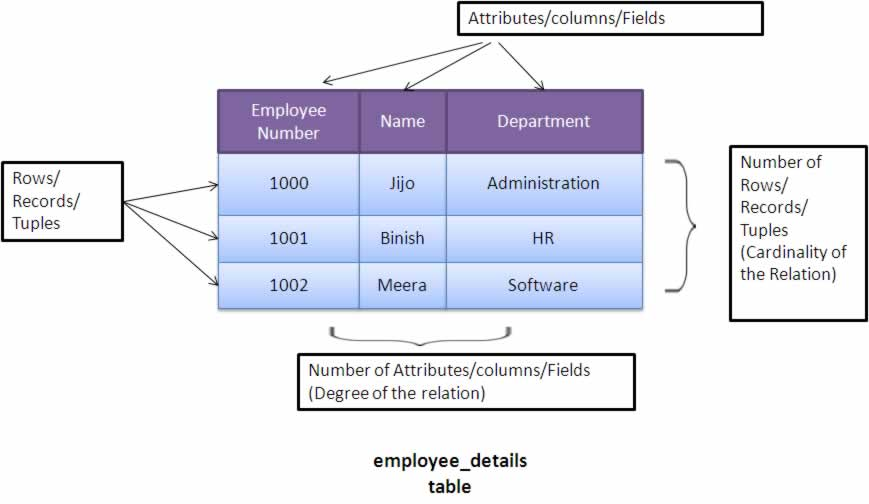
\includegraphics[width=0.6\linewidth]{mongodb_relational}
  \end{center}
  \caption{MongoDB: Relational Database Example.\\(Source: \url{http://www.careerbless.com/})}
\end{figure}
This model was so extended before NoSQL databases that a special-purpose semi-standard programming language was developed for these DBMS
(DataBase Management System). The relational model, while still very much prevalent in web development, has problems with horizontal
scalability (using networks of computers to host large databases, required specially for big data applications), performance (querying
speed is largely affected by the size of the database and the complexity of the query) and it can be overly complex in design. NoSQL
databases on the other hand tend to be much faster and scalable, with simpler models, but sacrifice some consistency when compared to
relational databases. This makes NoSQL adequate for applications that require large amounts of distributed data and applications that
require very fast read/write operations. HRUI in its current state, only requires the latter, as the database is the interface with
which controllers access and write data to and from the model (see section \ref{mvcpattern} on the Model-View-Controller pattern),
making the speed of database I/O crucial. In section \ref{scalability} of chapter \ref{futuredevelopment} the possibility of scaling
HRUI horizontally in future development is discussed.\\

MongoDB is a document-based database. This model is very simple, in that the database is merely a collection of objects (documents),
each containing data regarding each object. Each document can have any amount of attributes that can be completely unrelated to the
attributes of other documents. A MongoDB database is best described as a collection of objects or ``things'' without any obligation to
be related to one another. This makes it very simple to implement, as almost no restrictions apply to documents, in contrast with the
rigid nature of tables in the relational model.\\

MongoDB uses JSON (JavaScript Object Notation) to describe documents. Again, striving for simplicity, JSON can be defined very
succinctly (see \url{http://json.org/}), and is of course very well suited to use with Node.js, given that no translation is required
when reading and writing to the database. It should be noted that documents aren't stored in this format in MongoDB, using instead BSON
(Binary JSON), which transforms JSON into binary data for enhanced performance.
\begin{figure}[H]
\centering
\captionsetup{justification=centering}
\RecustomVerbatimEnvironment{Verbatim}{BVerbatim}{}
\begin{minted}{javascript}
{
    "_id": 0,
    "item": "joystick",
    "x": "0.00",
    "y": "0.00",
    "mode": "lock4ways"
}
{
    "_id": 2,
    "item": "robotGeolocation",
    "latitude": 40.496534,
    "longitude": -3.877457,
    "accuracyRadiusInMeters": "5"
}
{
    "_id": 4,
    "item": "profiles",
}
\end{minted}
\caption{MongoDB: HRUI Initial JSON Documents (abridged for brevity)}
\end{figure}
The fact that MongoDB uses JSON as a format, doesn't imply that it's only suitable for use with programs written in JavaScript. With SQL
not being a suitable language, MongoDB uses drivers to be accessed from programs, apart from the "mongo shell" interactive command line
tool. These drivers are essentially libraries that supply simple calls to query, insert, delete documents and so on from the database.
Drivers are available for all modern programming languages (C/C++, C\#, Java, Python...\cite{mongodb11}) and allow for simple, fast
communication with the database.
\begin{figure}[H]
\centering
\captionsetup{justification=centering}
\RecustomVerbatimEnvironment{Verbatim}{BVerbatim}{}
\begin{minted}{python}
#Import mongoDB driver
import pymongo
from pymongo import MongoClient
#Connect to MongoDB local instance
mongoclient = MongoClient()
db = mongoclient.hrui
data = db.data
#Obtain a Python dictionary representing the document
deviceData = data.find_one({"item": "deviceData"})
#use data
thrust = float(deviceData['devOrientation']['beta'])
\end{minted}
\caption{MongoDB: CrazyFlie Python Controller MongoDB usage (abridged for clarity)}
\end{figure}
This is specially useful for HRUI, as back-end controllers that read/write data from the model can be written in the developers choice
of language, making it extremely simple to integrate controllers for any robot, in any language. This decoupling of the user interface
with the actual robot controller will be discussed further in section \ref{mvcpattern} on the MVC pattern. On the other hand, although
the drivers are generally simple to use and implement, it would be better to have a universal solution like SQL, which is still the
biggest issue with NoSQL databases as opposed to SQL databases: lack of standardization and documentation. Still, it's very simple to
use a Python or Node.js script that extracts data from the database and relays it to whatever other program using RPC (Remote Procedure
Calls) software or middleware such as CORBA (Common Object Request Broker Architecture), or raw sockets. This circumvents using the more
cumbersome MongoDB drivers, while sacrificing some performance by using an interpreted language (generally negligible for most
applications). The latter is used in the Khepera III controller for control over a TCP/IP network and is briefly explained in section
\ref{kheperaIII}.
\newpage
\subsection{AngularJS} \label{AngularJS}
\begin{figure}[H]
\centering
\includesvg[width=0.7\linewidth]{./img/angularjs}
\caption{AngularJS Logo}
\end{figure}
AngularJS is a front-end web application framework that uses an MVC (Model-View-Controller) architecture for the design of client-side
applications. The MVC architecture implemented by AngularJS allows for very clear separation between declarative code and business
logic, keeping client-side applications well structured and modular. It's important to point out that the MVC pattern used by AngularJS
applies only to the front-end of the application, not the overarching architecture of the application as a whole, which is itself an MVC
paradigm.\\

In the AngularJS framework, declarative code stays separate from business logic. The declarative code (HTML) is the \textbf{View} in the
architecture, while business logic is implemented by \textbf{Controllers} (JavaScript). The controllers act upon the \textbf{Model},
which are a collection of JavaScript objects that are bound to the controllers scope (the parts of the model the controller has access
to). AngularJS then modifies the view dynamically when the model is changed. It's important to emphasize the difference between this
architecture and modifying the DOM (Document Object Model, see section \ref{HTML} for more) directly from JavaScript. When doing the
latter, there is no model, and thus no way of knowing what piece of code changed the DOM and why, leading to confusing, difficult to
maintain and inelegant code. With "the Angular way", the controller that has access to a certain part of the DOM is declared in HTML,
and more importantly, the variables that are bound in the DOM to the model are also explicitly declared in the HTML. By looking at the
HTML, one can instantly know which elements correspond to model variables, because they are declared as such. To do this, Angular has
custom attributes added to HTML tags. These attributes are called directives, and declare the behavior attached to the element in
question. For example the ``ngModel'' directive, attaches the value of an element to the value of a variable in the scope of a
controller. If this is attached to a checkbox, for example, when a user (considered a controller in the architecture) changes the state
of the checkbox by clicking it, the model will be updated and the variable in the scope of the controller will change to false or true
accordingly. The controller will then be able to use that model variable to implement the business logic that the change of state in the
checkbox requires. This is exactly what is done in HRUI, when checking modules on and off ("data-" prefix added to ng-model for HTML
Validation, as custom attributes require data- or x- prepended):
\begin{figure}[H]
  \captionsetup{justification=centering}
  \begin{center}
    
\includegraphics[width=0.5\linewidth]{angular_joystick}
  \end{center}
\end{figure}
\begin{figure}[H]
\centering
\captionsetup{justification=centering}
\RecustomVerbatimEnvironment{Verbatim}{BVerbatim}{}
\begin{minted}[fontsize=\footnotesize]{html}
<html data-ng-app="HRUI" data-ng-controller="HRUIController">
<!--...-->
<input id="joystickCheckbox" type="checkbox" data-ng-model="joystickOn"
data-ng-click="updateControls(event, joystickOn)">
<!--...-->
\end{minted}
\end{figure}
\begin{figure}[H]
\centering
\captionsetup{justification=centering}
\RecustomVerbatimEnvironment{Verbatim}{BVerbatim}{}
\begin{minted}[fontsize=\footnotesize]{javascript}
//...
app.controller('HRUIController', ['$rootScope', '$scope', 'SocketSrv', 'ProfileSrv',
    function(rootScope, scope, SocketSrv, ProfileSrv) {
        scope.joystickOn = false;
    //...
    //extract updated control from event, and notify back-end of selected controls
    scope.updateControls = function(control, newValue) {
        var changedControl = control.target.attributes.id.value;
        scope.sendControl(changedControl, newValue);
    };
\end{minted}
\caption{AngularJS: HRUI Checkbox Example (abridged for clarity)}
\end{figure}
In the HTML, the controller is declared (in this case for the entire document, as it's the master controller), and the directives are
assigned. The state of the checkbox (false equals unchecked) is bound to the scope variable joystickOn, which is initially false,
through the ngModel directive. The ngClick directive declares that the function called when the checkbox is clicked is updateControls,
that in this case sends the new state of the checkbox back to the server so it can process the actions that are necessary (sendControl,
not shown, uses Socket.IO to send the new value of the checkbox to the server via WebSockets. See section \ref{html5websockets} for
more).\\

This is just a small example of what can be achieved with what the creators of Angular call two-way data-binding. What this means is
that what is represented in the browser is simultaneously a variable in JavaScript, and can be modified by the user or controllers
indistinctly. The possibilities with this architecture are endless. Many of these directives are used in HRUI to create a dynamic 
single-page application very similar to what is expected of native desktop apps in terms of performance and responsiveness.\\

The concept of controllers that act upon different subsections of the DOM also allows for self contained modules to be added and removed
at will from an application, without the need to rewrite the whole JavaScript code. Since each controller is an independent entity, that
controls a part of the application without interference from other controllers, complex applications such as HRUI become very easy to
develop. The main benefits of this modularity are evident: once a module has been added and works correctly, more modules can be added
without any fear of breaking previous functionality, as there is no overlap in code; not all modules need to be active at any given
time, since each is independent, the user can select the relevant modules for each use-case on the fly; from a programmers perspective,
the code is very well compartmentalized making it easy to understand, maintain and improve upon; also from a programmers perspective,
code reuse is made simple, writing a controller once, using it in several parts of the application, or in other applications (following
the mantra DRY ``don't repeat yourself'. This is used in HRUI, with the same controller code attached to both joysticks, creating two
instances of the same controller); from a performance perspective, since modules are active only when they are used, there is no excess
resource usage.\\

Describing each of the directives used in detail would take up too much space, and would be hardly relevant to the subject at hand. Only
a couple of the more interesting directives used will be discussed briefly.
\begin{itemize}
  \item \textbf{ngIf}: The ngIf directive, allows elements to be added or removed from the DOM when the expression it evaluates is true
  or false respectively. This is a very important part of HRUI, that on startup seems empty, until the user starts turning modules on 
  (or loading a previously save profile, as explained in \ref{profilemanagement}) and these seem to appear in the browser. This is what
  allows the user to tailor the interface in a way that suits the use-case, and allows for performance to scale with the number of
  active modules.
  \item \textbf{ngAnimate}: This directive allows modules entering and exiting the application to have a visual effect when doing so.
  This uses a combination of CSS3 Transitions (see sections \ref{CSS} and \ref{html5styling}) and Pseudo-classes created by Angular to
  make modules fade-in and fade-out.
  \item \textbf{Custom Directive Touch}: The same way Angular lets the programmer create controllers, it allows the creation of custom
  directives. In HRUI, there is one custom directive used to add touch functionality to canvas elements (see section
  \ref{html5canvaselement}). This directive is bound to both the joystick canvases as wellas the map canvas, and uses handler functions
  to bind touch events to the equivalent mouse events. This is necessary only in canvas elements, as the rest of touch interactions are
  handled on the browser level.
  \begin{figure}[H]
  \centering
  \captionsetup{justification=centering}
  \RecustomVerbatimEnvironment{Verbatim}{BVerbatim}{}
  \begin{minted}[fontsize=\footnotesize]{javascript}
  app.directive('touch', function() {
      return {
          link: function(scope, element, attrs) {
              element.on('touchmove', function(event) {
                  scope.touchMove(event);
                  scope.$apply();
              });
              element.on('touchdown mousedown', function(event) {
                  scope.mouseDown(event);
                  scope.$apply();
              });
              element.on('mousemove', function(event) {
                  scope.mouseMove(event);
                  scope.$apply();
              });
              element.on('mouseup touchend', function(event) {
                  scope.mouseUp(event);
                  scope.$apply();
              });
          }
      }
  });
  \end{minted}
  \end{figure}
  \begin{figure}[H]
  \centering
  \captionsetup{justification=centering}
  \RecustomVerbatimEnvironment{Verbatim}{BVerbatim}{}
  \begin{minted}[fontsize=\footnotesize]{html}
  <canvas id="joystick" class="canvas joystick" data-touch>
  <canvas id="joystick2" class="canvas joystick" data-touch>
  <canvas id="mapcanvas" class="canvas" data-ng-show="mapOn" data-touch>
  \end{minted}
  \caption{AngularJS: HRUI Touch Directive (HTML abridged for clarity)}
  \end{figure}
  \item \textbf{Custom Directive Compile}: This directive allows the generation of HTML dynamically. This is required in the Custom 
  Input module (see section \ref{custominput}) to generate the HTML controls that the user has required. With the form data entered by 
  the user detailing what kind of inputs are required, an HTML table is created (function generateInputTable) that then needs to be 
  compiled into the DOM with the data-bindings to the model required. It's somewhat complex, but it allows for custom inputs to be 
  generated on the fly, adding great versatility to the interface.
    \begin{figure}[H]
  \centering
  \captionsetup{justification=centering}
  \RecustomVerbatimEnvironment{Verbatim}{BVerbatim}{}
  \begin{minted}[fontsize=\footnotesize]{javascript}
  app.directive('compile', function($compile) {
    return function(scope, element, attrs) {
        scope.$watch(
            function(scope) {
                // watch the 'compile' expression for changes
                return scope.$eval(attrs.compile);
            },
            function(value) {
                // when the 'compile' expression changes
                // assign it into the current DOM
                element.html(value);

                // compile the new DOM and link it to the current
                // scope.
                $compile(element.contents())(scope);
            }
        );
    };
  });
  \end{minted}
  \end{figure}
  \begin{figure}[H]
  \centering
  \captionsetup{justification=centering}
  \RecustomVerbatimEnvironment{Verbatim}{BVerbatim}{}
  \begin{minted}[fontsize=\footnotesize]{html}
  <table id="customInputTable" class="table" data-compile="customInputTable" 
  data-ng-if="customInputFormSubmitted"></table>
  \end{minted}
  \caption{AngularJS: HRUI Compile Directive}
  \end{figure}
\end{itemize}
Apart from controllers and directives, Angular (among many other features that are outside the scope of this report) implements 
services, to allow for communication between controllers, without interfering with each others scope. Services are "singletons" (in 
object-oriented programming, classes that can only have one instance at runtime) that contained shared methods or shared data. 
Controllers can claim access to a service and modify or bind to its data as well as call its functions. Since there's only one instance 
of a service, sharing data between controllers is reduced to writing or binding a service attribute and reading it from another 
controller. It also allows for code reuse (DRY ``don't repeat yourself') with functions that are used in several controllers being coded 
only once. There are 4 services in HRUI:
\begin{itemize}
  \item \textbf{ProfileSrv}: Allows controllers to publish the state of their scopes to the master controller, that then creates a
  profile with these states that can then be saved in the back-end for future use. See section \ref{profilemanagement} for more.
  \item \textbf{SocketSrv}: Holds the Socket.IO Websocket connection that needs to be accessed from all controllers to receive and emit
  events to the back-end, as well as media streaming raw WebSockets. See section \ref{html5websockets} on WebSockets.
  \item \textbf{DrawSrv}: Contains functions used to draw in Canvas elements: drawCircle, drawLineFromCenter and writeInCanvas (used in
  previous iterations).
  \item \textbf{GeometrySrv}: Contains functions used to calculate coordinates in Canvas elements: isInsideCircle, forceIntoCircle,
  centerCoord, canvasCoord, forceDirectionLock.
\end{itemize}
  \begin{figure}[H]
  \centering
  \captionsetup{justification=centering}
  \RecustomVerbatimEnvironment{Verbatim}{BVerbatim}{}
  \begin{minted}[fontsize=\footnotesize]{javascript}
  //Service with typical drawing methods shared between controllers
  app.service('DrawSrv', function() {
      return {
          drawCircle: function(ctx, x, y, radius, fillColor) {
              ctx.beginPath();
              ctx.arc(x, y, radius, 0, 2 * Math.PI, false);
              if (!!fillColor) { //if fillColor arg given, fill in circle.
                  ctx.fillStyle = fillColor;
                  ctx.fill();
              };
              ctx.stroke();
          },
          drawLineFromCenter: function(ctx, x, y) {
              ctx.beginPath();
              ctx.moveTo(ctx.canvas.width / 2, ctx.canvas.height / 2);
              ctx.lineTo(x, y);
              ctx.stroke();
          },
          writeInCanvas: function(ctx, font, text, x, y) {
              ctx.font = font;
              ctx.fillText(text, x, y);
          },
      }
  });
  \end{minted}
  \caption{AngularJS: HRUI DrawSrv Service example}
  \end{figure}
A full recap of the features of AngularJS is far beyond the scope of this report, but suffice it to say it's one of the core
technologies of this project, as the previous brief examples have shown. Without AngularJS, the Single-page Application wouldn't be as
responsive and immediately easy to use; the front-end code would be much less readable and as a result much more difficult to maintain
and build upon. As it is, a new front-end module can be added to the application very fast, so much so that the modules added later in
the development (gamepad, device motion and voice commands) took just a few hours to develop on the front-end, in part because of the
excellent modularity provided by the AngularJS framework that had been implemented previously. AngularJS is supported by Google and has
extensive and exhaustive documentation online\cite{google10}, both of which make it a very reliable framework to use, although a bit
daunting at first.
\newpage
\section{Development Environment \& Tools}
This section briefly describes the software development environment, software tools used to develop the project as well as
the robots used to demonstrate the integration of the project with existing hardware and simulated robots. The development
environment comprises the operating system (OS) used for development and deployment of the project, the source code editor
and build management software as well as the revision control system.
\subsection{Linux} \label{linux}
\begin{figure}[H]
\centering
\subfloat{\includesvg[width=0.2\linewidth]{./img/tux}}
\subfloat{\frame{\includesvg[width=0.6\linewidth]{./img/mint}}}
\caption{Tux the penguin, Linux mascot and Linux Mint Official Logo}
\end{figure}
Linux is the OS of choice for software development. The Linux distribution used in this project is Linux Mint 17 (Qiana) - 17.1(Rebecca)
Cinnamon Edition (64-bit version), that is based on the Ubuntu distro, itself based on Debian. A description of the Linux kernel and the
distribution used in this project is far beyond the scope of this report, but the choice to develop and deploy the application on this
platform will be discussed briefly.\\

The main reason why this project was developed on Linux is because of how easy it makes the installation and use of development tools 
through package management systems. A package management system automatically installs software and all of its dependencies (external 
software a program relies on to function) without having to manually download or install anything. This makes installing the needed 
software to develop this project as simple as  executing the command: \mintinline{shell}{ sudo apt-get install nodejs npm mongodb python2
}, which will install any dependencies required and will configure the programs for use. In Microsoft Windows, no official package 
management is implemented (although third-party package managers exist, like "chocolatey"), so installation and configuration of node, 
npm, python and mongodb has to be performed manually, with the ensuing troubleshooting. This applies to most Linux distributions, making 
it very simple to translate the installation and development requirements from one distribution to another. The Raspberry Pi 2 (see 
section \ref{raspberrypi2}) used as a portable server in this project, uses an Arch Linux distribution, but the installation is roughly 
the same: \mintinline{shell}{ sudo pacman -Syu install nodejs npm mongodb python2}, using the Pacman package manager. This portability 
offered is just one of the many reasons (configurable, wealth of development tools, command-line interface, scripting, etc.) that Linux 
is the main software development platform of the world.

The application is designed to work best on a Linux server, like the majority of web servers publicly accessible on the Internet.
However, given that one of the objectives of the project is accessibility to both the front-end of the application and the back-end, the
server works on any machine capable of running Node.js (see section \ref{nodejs}) and MongoDB (see section \ref{mongodb}). The only
caveat to the use on systems other than Linux is the loss of media streaming capabilities, that rely on Linux dev files to access video
and audio hardware. The main reason Linux is used as a server platform is for its stability and reliability. Windows machines require
regular maintenance and reboots to work properly while Linux is generally much more stable.
\subsection{Sublime Text}
\begin{figure}[H]
\centering

\includegraphics[width=0.2\linewidth]{sublime}
\caption{Sublime Text Logo}
\end{figure}
Sublime Text is the text and source code editor used in this project. It's not a traditional IDE (Integrated Development
Environment) like Eclipse or NetBeans, but includes many of the features found in those, implemented through user developed
plug-ins that are installed through a package management system of it's own: Package Control. Some of these features are:
\begin{itemize}
  \item Project file management: Create custom project file trees to access on the fly from the sidebar.
  \item Multiple editor tabs and file map: Edit code side by side, very useful when developing front-end and back-end of a module in
  HRUI, and visual map of file on the right side of the screen for quick scrolling, useful for tracking sections in code or in \LaTeX
  source.
  \item Customizable build systems: Create scripts that run custom commands to build or execute the source.
  \item Language-specific code highlighting and coloring: Helps visual orientation in code.
  \item Automatic code formatting: Runs a script that automatically refactors the code for readability, with correct indentation and
  trailing spaces.
  \item Code completion and code snippets: Auto-completes variable, function and typical programming structures (functions, objects, 
  if-else if) for convenience.
  \item Refactoring tools: Make changes to code that affect several parts of the project instantly, e.g. changing a variable name across
  the whole application once, instead of in each instance of the name.
  \item Version control integration: Run version control (see section \ref{git}) commands directly from the editor.
  \item Scripting tools: Such as a CSS auto vendor prefixer (adds vendor specific prefixes to CSS code automatically when including a
  conflicting CSS rule) or javascript/CSS minifier (reduces the size of javascript/CSS files by refactoring text, saving network
  resources).
  \item Aesthetic customization: Modify the UI for visual comfort.
\end{itemize}
Sublime Text was used for both the development of the source code as well as for this report in \LaTeX.
\begin{figure}[H]
\centering
\subfloat{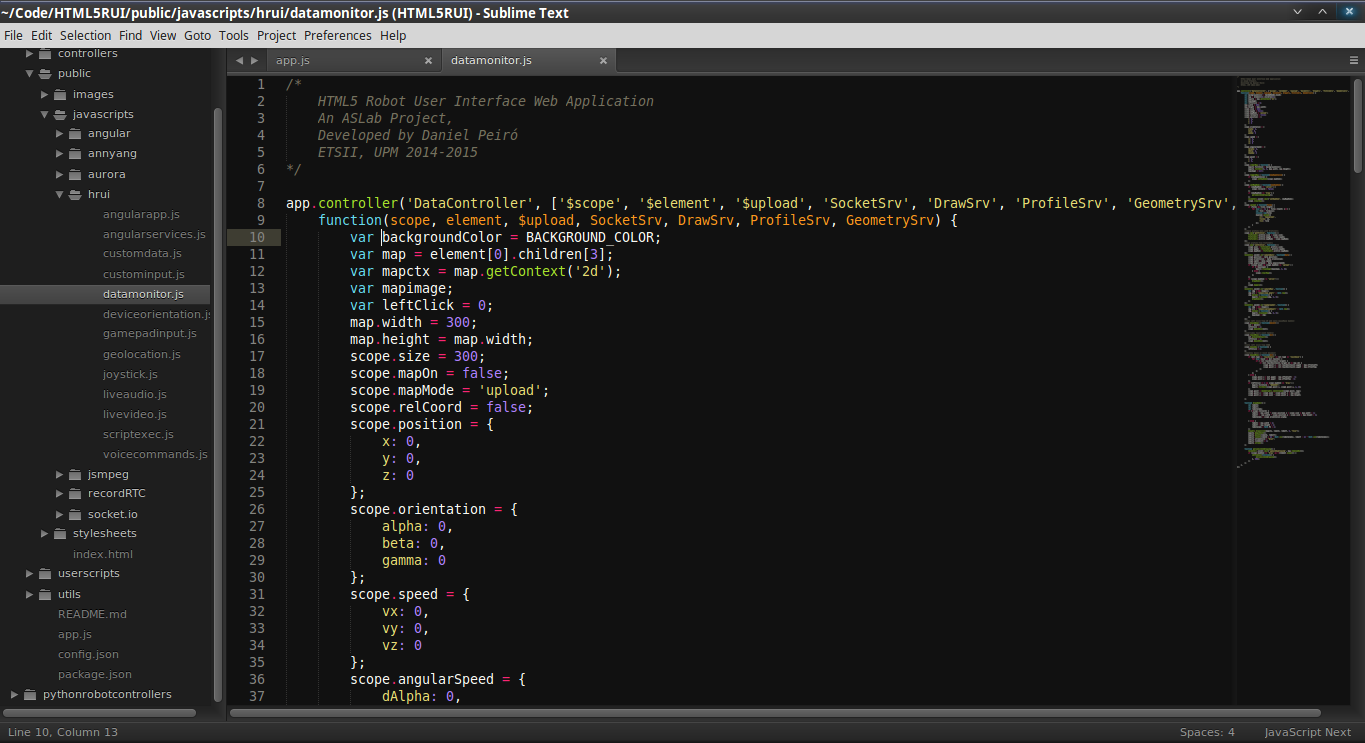
\includegraphics[width=0.5\linewidth]{sublime_hrui}}
\subfloat{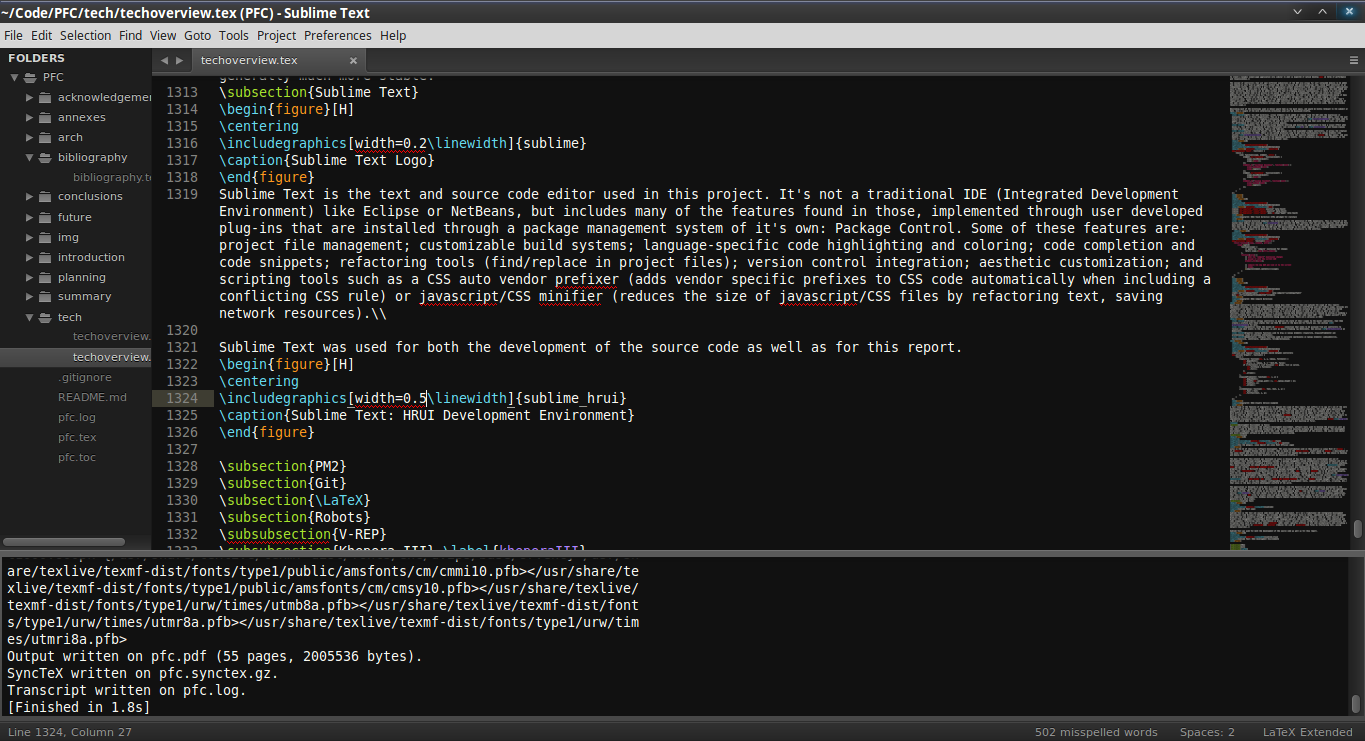
\includegraphics[width=0.5\linewidth]{sublime_report}}
\caption{Sublime Text: HRUI and Report Development Environment}
\end{figure}
\subsection{PM2}
\begin{figure}[H]
\centering

\includegraphics[width=0.6\linewidth]{pm2}
\caption{PM2 Logo}
\end{figure}
PM2 is a process manager that supplies Apache-like server management. Node.js (see section \ref{nodejs}) creates the possibility of
lightweight asynchronous web servers through frameworks like Express (see section \ref{express}). This is very useful, but Node is still
just a process on a server: if for whatever reason the application crashes or the server restarts, there is no service that restarts the
application or starts the web server on boot. That is where programs like PM2 come in, keeping the web server running, balancing its
load and restarting it if need be. It also has process monitoring and management options. PM2 is itself installable through the Node
Package Manager, NPM, as it is a Node.js module.\\

With PM2 the application can be set to start on boot, and restarted automatically if any crashes occur, with a 0 s reload downtime,
giving a reliable solution for long term use of the server. This is used in this project to implement the portable server using the
Raspberry Pi 2 (see section \ref{raspberrypi2}). PM2 is configured in the embedded Linux OS to start the app on boot and keep it alive,
allowing the board to act as an ``out of the box'' server for use anywhere with no configuration, except connection to a given network
via Ethernet or Wifi.\\

PM2 was also used throughout the development of the application, taking advantage of its file monitoring capabilities. PM2 can be
configured to restart the application if any of the files in its directory are modified. This was extremely useful in creating an agile
workflow for development. The PM2 service was started with this option enabled and the server would start. Modifications and additions
were made to the source code and upon save, PM2 would detect the change and restart the application wit the new source automatically.\\

Other PM2 features used throughout development were its memory and CPU monitoring and logging tools. Logging showed the console output
of the app for debugging and the monitoring feature helped detect memory leaks and inefficiencies in testing.
\begin{figure}[H]
\centering
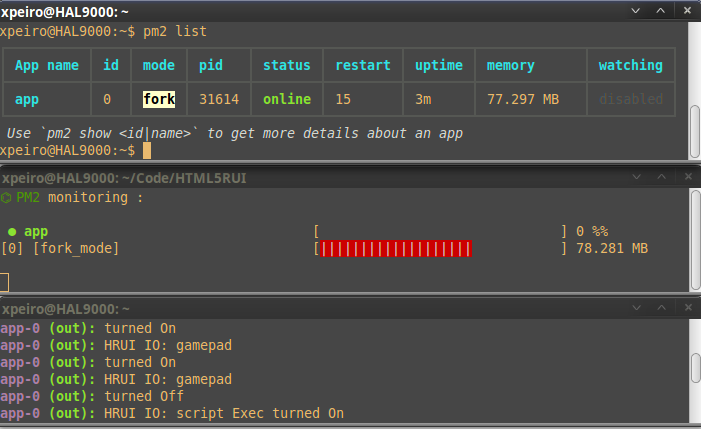
\includegraphics[width=0.6\linewidth]{pm2example}
\caption{PM2: PM2 list, monit and logs command output example}
\end{figure}
\subsection{Git \& GitHub} \label{git}
\begin{figure}[H]
\centering
\subfloat{
\includegraphics[width=0.3\linewidth]{git}}
\subfloat{
\includegraphics[width=0.4\linewidth]{github}}
\caption{Git and Github Logo}
\end{figure}
Git is a distributed revision control system developed by Linus Torvalds, the creator of the Linux Kernel. A revision control system is
used in software development to track changes to the source code of a project. The distributed nature of Git allows multiple developers
to work on a project merging the changes made by all of them to a single or multiple versions of the code, keeping track of all changes,
so that they can be automatically reversed or superseded if necessary. This aspect of Git wasn't used in this project, as there was only
one developer, but revision control is also useful in this use-case. With Git, a code repository is created, wherein all of the code is
placed. The code in the repository is tracked for changes, and when the developer deems it appropriate (normally when a large change or
several smaller changes are made to the code), the changes are "committed" to Git. This ``commit'' is then "pushed" to the repository,
establishing a new version of the code, with a short message attached to it, explaining the changes. The cycle then restarts. For multi-
developer projects, another step is required: ``pulling'' the latest version from the repository  before making changes. If this is not
done, the changes can be ``merged'' if the changes do not conflict with the latest commit.\\

GitHub is a web service that hosts public Git repositories free of charge. It also maintains statistics on the development and the code,
 some of which are used in section \ref{planning} on Project Planning. GitHub was used in this project to host both the 
\href{https://github.com/xpeiro/HTML5RUI}{project repository} as well as \href{https://github.com/xpeiro/PFC}{this report's repository}, 
as well as for the use of public repositories for the JavaScript MPEG1 decoder \href{https://github.com/phoboslab/jsmpeg}{JSMpeg}, the 
Voice recognition library \href{https://github.com/TalAter/annyang}{Annyang} and the MP3 JavaScript decoder 
\href{https://github.com/audiocogs/aurora.js/}{Aurora.js} and their respective documentation. GitHub also allows the possibility of
hosting static web pages. This features is used to include a version of the User Manual (see section \ref{usermanual}) online at: 
\url{http://xpeiro.github.io/hrui/index.html}.\\

Revision control in general has many benefits:
\begin{itemize}
  \item Revert changes that result in issues: Since all previous versions are stored, the code can be reverted to any previous version
  very simply.
  \item Detect source of issues: When a bug or issue with the application arises that was not previously present, revision control can
  make it very easy to pinpoint which commit created the problem, by testing previous versions and testing which one first had the bug,
  making debugging easier.
  \item Backup: By using a hosting service like GitHub the code is protected from local hardware/software failures and errors. In
  distributed revision control, several copies of the code exist at any given time on different servers.
  \item Code history or statistics: analysis of work load and work performance is easier with data on who changed the code, when, why
  and how many times.
  \item Compartmentalization: Experimental changes to code can be made without affecting a working version of the code, eliminating
  chances of breaking code inadvertently.
  \item Sharing: services like GitHub make sharing code very simple.
\end{itemize}
\subsection{\LaTeX}
\LaTeX\ (pronounced ``Lah-tech'') is an open source procedural markup language for document preparation originally developed by Leslie
Lamport based on the \TeX typesetting system by Donald Knuth. It's widely used to create scientific and technical documentation, such as
this report. It's comprised of a series of macros (text that is processed to be replaced with other text) for the underlying \TeX\
typesetting system. It has several advantages over the more common WYSIWYG (``What You See Is What You Get'') word processors like
Microsoft Word (the de facto alternative):
\begin{itemize}
  \item Separation between content and presentation: The content is not tied to the presentation, rather the presentation can be changed
  using macros without modifying the content, which is simple text.
  \item Referencing: Powerful tools are available to make cross references in large documents like the ones made in this document when
  referring to sections.
  \item Automatic Numbering and Indexing: The cross references made do not make reference to the numbers of the sections. This numbering
  is generated by \LaTeX\ automatically and references are macros that fill in with the correct number on compilation. This is also used
  for the bibliography.
  \item Automatic Table of Contents and Figures: The table of contents is auto generated with the sections on compilation. Likewise the
  table of figures is generated with the existing figures (also numbered automatically).
  \item Better content embedding: Inserting images and graphics is much simpler and organized.
  \item Development Community: Creates hundreds of packages that are useful for all kinds of different use-cases whereas commercial
  solutions require limited features for broad appeal.
  \item Compatibility: \LaTeX\ source from 20 years ago can still produce a document today. Word documents cannot, without significant
  modifications.
  \item Revision Control: \LaTeX\ source can be easily put under version control, whereas this feature in Microsoft Word is very limited.
  \item Source readability: Word .docx files are essentially zipped XML, which is very hard to read. \LaTeX\ commands on the other hand
  are very close to their meaning and do not interfere with the content as much.
  \item Source Commenting: Adding comments to the source, more information can be added on how the document should be presented and why.
  \item Open Source: Can be modified at will with added packages that provide new functionalities.
\end{itemize}
  \begin{figure}[H]
  
  \captionsetup{justification=centering}
  \RecustomVerbatimEnvironment{Verbatim}{BVerbatim}{}
  \begin{minted}[fontsize=\footnotesize]{latex}
%   HTML5 Robot User Interface Project Report
%   An ASLab Project,
%   Developed by Daniel Peiró
%   ETSII, UPM 2014-2015

% Define Document Type, Font size, Paper size, and input/output encoding.
\documentclass[12pt,twoside,a4paper]{report}
\usepackage[T1]{fontenc} 
\usepackage[utf8]{inputenc}

%%%%%%% Formatting Section %%%%%%%%

% Document formatted according to PR/CL/1/001,
% Annex ANX-PR/CL/1/001-01, available at:
% http://www.industriales.upm.es/la_escuela/doc/Procedimiento-TFG-TFM-PFC-def.pdf
%
% Font: Times New Roman, 12 points.
% Margins: All 1 in.
% Header and footer content: Defined in 'plain' page style. 

\usepackage{mathptmx} % Times New Roman.
\usepackage[top=1in, bottom=1in, left=1in, right=1in]{geometry} % 1 in. Margins.
\usepackage{fancyhdr} % Header/Footer formatting.
  \end{minted}
  \end{figure}
  \begin{figure}[H]
  
  \captionsetup{justification=centering}
  \RecustomVerbatimEnvironment{Verbatim}{BVerbatim}{}
  \begin{minted}[fontsize=\footnotesize]{latex}
\pagestyle{plain} %Set Document Page Style to plain
\setlength{\headheight}{15pt} % Header height 15 points.
\setcounter{tocdepth}{4} % Set Table of Contents sectioning depth
\setcounter{secnumdepth}{4} % Set Table of Contents numbering depth
\fancypagestyle{plain}{
    \fancyhf{} %Clear Defaults.
    \renewcommand{\headrulewidth}{1pt} % Header horizontal rule.
    \renewcommand{\footrulewidth}{1pt} % Footer horizontal rule.
    \fancyhead[LE]{\nouppercase\leftmark} % Even Pages: Chapter and Section Name, top left.
    \fancyfoot[LE]{\thepage} % Even Pages: Page number, bottom left.
    \fancyfoot[RE]{Escuela Técnica Superior de Ingenieros Industriales (UPM)} 
    % Even Pages: University name, bottom right.
    \fancyhead[RO]{HTML5 Robot User Interface} % Odd pages: Project name, top right.
    \fancyfoot[RO]{\thepage} % Odd pages: Page number, bottom right.
    \fancyfoot[LO]{Daniel Peiró Moreno}  % Odd pages: Author, bottom left.
}
%%%%% End Formatting Section %%%%%%

% Title, Author and Date
\title{HTML5 Robot User Interface}
\author{Daniel Peiró Moreno}
\date{2015}

%%%%%% Import Packages %%%%%%
\usepackage{graphicx}
\usepackage{svg}
\usepackage{subfig}
\usepackage{epigraph}
\usepackage{hyperref}
\usepackage{makeidx}
\usepackage{minted}
\usepackage{lipsum}
%%%% End Import Packages %%%%

\begin{document}

% 	HTML5 Robot User Interface Project Report: Acknowledgements
% 	An ASLab Project,
% 	Developed by Daniel Peiró
% 	ETSII, UPM 2014-2015

\chapter*{}
\vspace{120pt}
\epigraph{\textit{Para Cristina, por hacerlo posible.}}{}
\vspace{90pt}
\epigraph{\textit{Ex Nihilo Nihil Fit.\\
Out of nothing, nothing becomes.}}{\textit{Titus Lucretius Carus\\De Rerum Natura}}

\tableofcontents
% 	HTML5 Robot User Interface Project Report: Summary
% 	An ASLab Project,
% 	Developed by Daniel Peiró
% 	ETSII, UPM 2014-2015
\chapter*{Resumen Ejecutivo\\(Executive Summary in Spanish)}

El objetivo de este proyecto es el desarrollo de \textit{software} que proporcione una interfaz gŕafica de usuario (en adelante 
\textit{GUI}) con una variedad de herramientas diseñadas para recoger entradas (\textit{inputs}) para el control de robots, asi 
como la presentación de las salidas (\textit{outputs}) de los mismos. Se desea que la aplicación (el programa) cumpla con los 
siguientes requisitos:
\begin{itemize}
	\item \textbf{Universalidad}: La GUI debe ser fácilmente adaptable al uso de un amplio abanico de robots, con diferentes 
	capacidades y características.
	\item \textbf{Accesibilidad}: Este requisito se divide en dos partes:
	\begin{itemize}
		\item La GUI debe ser fácilmente utilizable desde un amplio abanico de dispositivos, incluyendo como mínimo, 
		ordenadores de sobremesa (\textit{desktop}) y portátiles (\textit{laptop}), dispositivos móviles como teléfonos 
		inteligentes (\textit{smartphones}) y tabletas (\textit{tablets}), todos ejecutando distintos sistemas operativos, con 
		respecto a los cuales la aplicación debería ser agnóstica (debería ejecutarse indistintamente en cualquier SO).		
		\item La aplicación que proporcione la GUI debe además exponer una API (\textit{Application Programming Interface} o 
		Interfaz de Programación de la Aplicación) que permita a desarrolladores externos usar las entradas y salidas de la GUI 
		para cualquier robot o aplicación, consiguiendo asi realizar el primer requisito. Esta interfaz debe ser tan simple 
		como sea posible, y debe cumplir con todos los demás requisitos, donde sea aplicable (por tanto debe ser portable, 
		distribuida, en tiempo real y de código abierto (\textit{open source})).
	\end{itemize}
	\item \textbf{Personalizable (\textit{Customizable})}: Parcialmente debido al primer requisito, la GUI debe tener una 
	variedad de entradas y salidas que deben ser utilizables de manera independiente, de tal forma que múltiples 
	configuraciones puedan prepararse y ser usadas para diferentes robots, asi como para diferentes aplicaciones del mismo 
	robot. A ser posible, el usuario debería poder crear entradas y salidas personalizadas cuando las herramientas propuestas 
	sean insuficientes para la aplicación particular. Este proceso debería ser sencillo y transparente para el usuario, a ser 
	posible.
	\item \textbf{Distribuida}: Parcialmente debido al requisito de accesibilidad, la aplicación debe ser distribuida en red, de 
	manera que la GUI no esté físicamente atada a una máquina en particular, o tenga que ser ejecutada de manera local para 
	aportar la funcionalidad requerida.
	\item \textbf{Tiempo Real}: Las entradas registradas por la GUI deben ser capaces de controlar al robot en tiempo real. 
	Asímismo, las salidas del robot deben ser presentadas al usuario en tiempo real. No se establecen tiempos límite 
	(\textit{deadlines}) severos, dado que la aplicación es distribuida y por tanto estos tiempos serían difíciles de estimar sin 
	una investigación exhaustiva y control sobre el entorno de ejecución de la aplicación, lo cual negaría el requisito de 
	accesibilidad. Sin embargo, el tiempo de respuesta del sistema deberá minimizarse dentro de las posibilidades del estado del 
	arte de las tecnologías empleadas.
	\item \textbf{Portabilidad}: La aplicación que proporcione la GUI debe ser ejecutable en un amplio abanico de sistemas, con 
	respecto a estas variables:
		\begin{itemize}
			\item Prestaciones \textit{Hardware}: La aplicación debe ser ejecutable en ordenadores portables de bajo coste y 
			bajas prestaciones con el fin de ser montable sobre robots móviles si así se requiere.
			\item Sistemas Operativos: La aplicación debe ser multi plataforma, es decir, debe ser ejecutable en una variedad de 
			sistemas operativos. Estos SOs deben incluir, como mínimo: una distribución de uso general de Linux, Microsoft 
			Windows y Apple OS X. Solo las últimas versiones de cada uno deben ser soportadas. Se requiere soporte como mínimo 
			las siguientes arquitecturas: 32/64-bit x86.\\
		\end{itemize}
	\item \textbf{Código Abierto (\textit{Open Source})}: Todo el \textit{software}, bibliotecas (\textit{libraries}) y 
	\textit{frameworks} empleados en el desarrollo y uso de la aplicación deben ser de código abierto. Esto, a grandes rasgos, 
	supone que el \textit{software} sea libre para el uso, estudio y modificación del mismo para cualquier propósito. Las 
	implicaciones del código abierto se estudian en la memoria del proyecto como valoración de los impactos y aspectos de 
	responsabilidad legal, ética y profesional del trabajo. Las herramientas usadas para el desarrollo (Entornos Integrados de 
	Desarrollo \textit{IDEs}, SOs, \textit{hardware} etc.) no tienen porque ser de código abierto, pero se preferirán 
	herramientas que lo sean en caso de ser alternativas viables.\\
\end{itemize}
En esencia, la aplicación debe establecer un nexo entre las dos entidades principales del control de robots:
\begin{itemize}
	\item \textbf{El Usuario}: Requiere una interfaz para introducir comandos que el robot debe seguir. Asímismo, requiere una 
	vista de las datos de salida del robot, si están disponibles.
	\item \textbf{El Robot}: Necesita recibir comandos en un protocolo particular que entiende, para poder funcionar. Además, 
	opcionalmente, puede exponer datos de salida para que el usuario los vea o sean registrados.
\end{itemize}
En el siguiente diagrama UML (\textit{Unified Modeling Language}) simplificado,se muestran los tres componentes: el usuario, la 
aplicación y el robot. El objetivo del proyecto es el desarrollo del componente central, la aplicación, junto con las interfaces 
que expone tanto al usuario como a robot, o con mayor precisión al controlador del robot, que traducirá la interfaz de la 
aplicación a la interfaz que entiende el robot.
\begin{figure}[H]
\centering
\captionsetup{justification=centering}
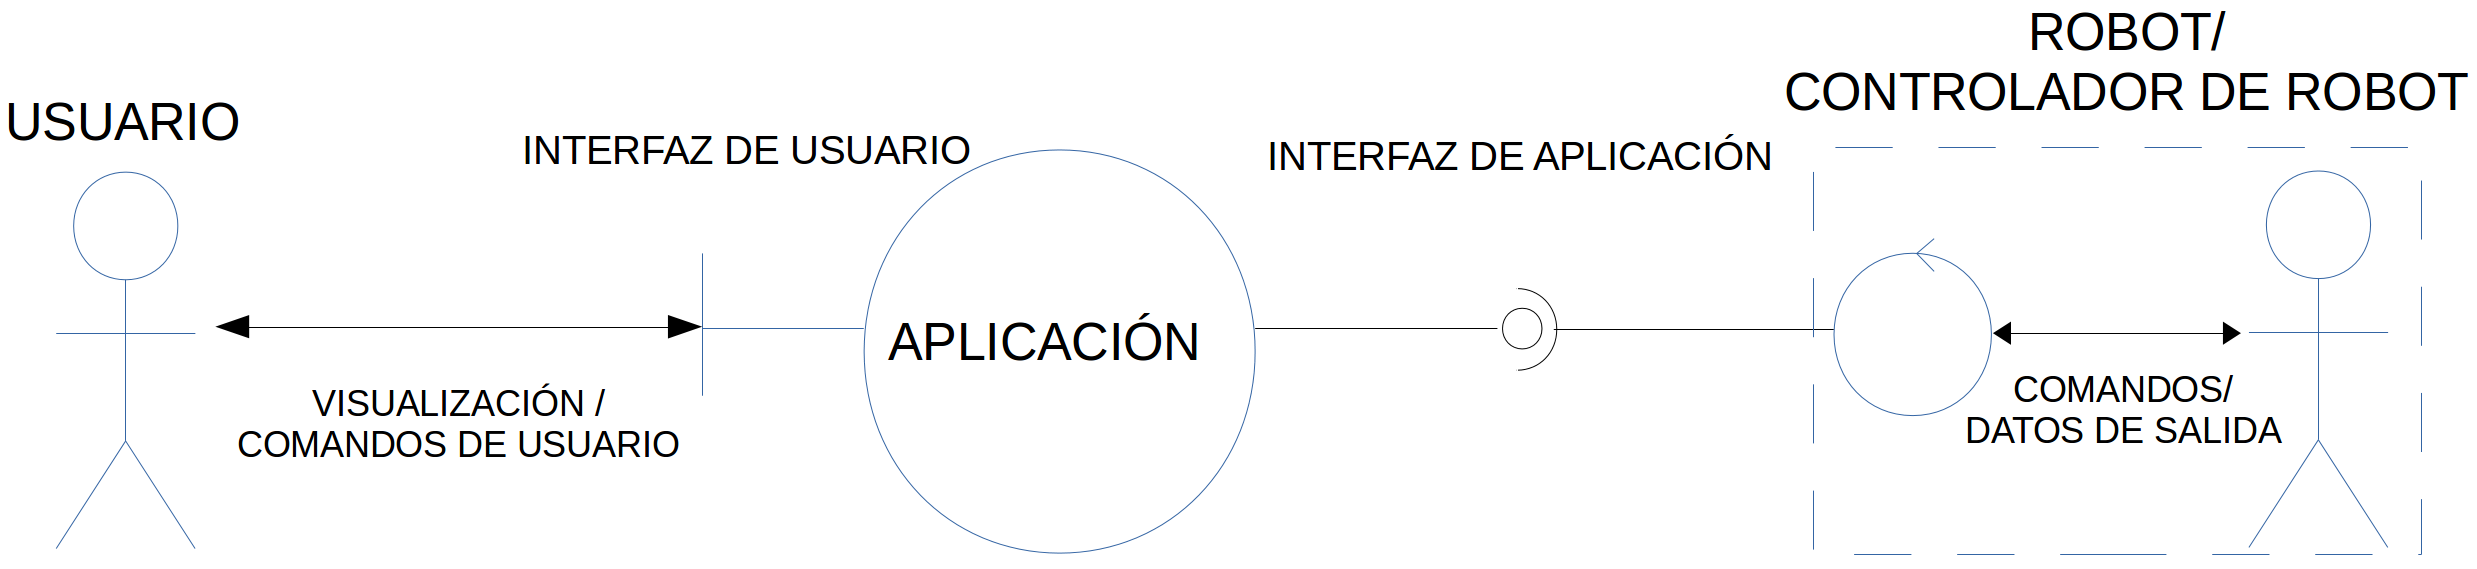
\includegraphics[width=\linewidth]{resumenuml}
\caption{Diagrama UML simplificado del objetivo del proyecto}
\end{figure}

Siguiendo un esquema de desarrollo en cascada iterativo (elaboración de requisitos, diseño, implementación y verificación, 
iterados para cada módulo de la aplicación, y finalmente mantenimiento), se planificó el proyecto. A continuación se procedió al 
estudio del estado del arte de las tecnologías que cumplen con estos requisitos y el diagrama de objetivos. Se diseñó una 
arquitectura del sistema que cumplía con los objetivos y se desarrolló la aplicación. Por último se probó el funcionamiento de la 
aplicación y se escribió la memoria del proyecto, en la que se describe en detalle el estado del arte de las tecnologías 
empleadas (capítulo 2), la arquitectura del sistema (capítulo 3), el desarrollo futuro (capítulo 4) y la planificación del 
proyecto (capítulo 5). Se incluye además como anexo el manual de usuario de la aplicación.\\

Los puntos básicos de la solución propuesta son los siguientes:
\begin{itemize}
	\item \textbf{GUI Modular en HTML5}: La GUI es una página web estrictamente en HTML5 (la última versión del estándar del 
	lenguaje empleado para diseñar páginas web). Esto propone una solución al requisito de accesibilidad, dado que las páginas 
	HTML5 son accesibles desde cualquier dispositivo capaz de abrir una página web. Esto incluye ordenadores, teléfonos 
	inteligentes y tabletas, así como una variedad de micro ordenadores. La modularidad proporciona una solución al requisito de 
	personalización, dado que cada módulo puede ejecutarse independientemente de otros, y por tanto cualquier permutación de 
	módules es posible.
	\item \textbf{Servidor Node.js}: La aplicación es un servidor web Node.js (una plataforma para ejecutar programas en el 
	lenguaje JavaScript como si fueran cualquier otro programa, en lugar de en el navegador. Está basado en el motor de 
	JavaScript de Google Chrome, es muy ligero y asíncrono). Dado que Node.js es multi plataforma, esto también aporta una 
	solución al requisito de portabilidad.
	\item \textbf{Arquitectura Cliente-Servidor}: Proporciona una solución al requisito  de ser una aplicación distribuida. El 
	clientes es la página web HTML5. El servidor es la aplicación que maneja las entradas y salidas del cliente. Pueden ser 
	ejecutados en máquinas distintas y se comunican vía Internet o en red local mediante varios protocolos.
	\item \textbf{Comunicación basada en \textit{WebSockets}}: Este protocolo de comunicación permite al cliente y servidor 
	comunicarse en tiempo real sobre una red de manera eficiente pasando mensajes entre ellos con paquetes de datos asociados, de 
	manera similar a los programas que se comunican entre sí mediante un \textit{socket} UNIX. Esto da respuesta al requisito de 
	tiempo real.
	\item \textbf{Arquitectura MVC (Modelo-Vista-Controlador)}: Propone una solución a los requerimientos de universalidad y 
	accesibilidad (segundo apartado), mediante el diseño de la aplicación. Se diseña de manera que la GUI (la Vista) está 
	desacoplada del estado de la aplicación (el Modelo), permitiendo así que desarrolladores externos accedan sencillamente al 
	Modelo, usando Controladores. Esto se llama doble-desacoplamiento (\textit{double-decoupling}) en el proyecto.
	\item \textbf{Entradas y salidas personalizables}: Como resultado de la prestación previa, el usuario puede crear nuevas 
	entradas y salidas dinámicamente, que son accesibles a la interfaz de la aplicación de manera instantánea y transparente. 
	Esto da respuesta al requisito de personalización.
	\item \textbf{Código abierto}: Todas las tecnologías empleados son de código abierto.
\end{itemize}
Los resultados del proyecto se detallan en el capítulo 6 de la memoria.\\

Como demostración del funcionamiento de la aplicación, se realizó la integración de la misma con tres robots distintos:
\begin{itemize}
	\item \textbf{Khepera III Virtual, en simulador V-REP}. Comunicado en Red.
	\item \textbf{Khepera III (Robot diferencial)}. Comunicado en Red inalámbrica.
	\item \textbf{Crazyflie 2.0. (Mini-Cuadrirotor)}. Comunicación por Radio.
	\item Parrot Rolling Spider (Mini-Cuadrirotor con estabilización de altura por ultra-sonidos). Comunicación por bluetooth. 
	(Nota: no documentado por ser muy parecido al anterior cuadrirotor).
\end{itemize}

Siendo las tres integraciones un éxito, ya que con controladores relativamente simples (el cuadrirotor requiere apenas 50 líneas 
de código para ser controlado totalmente en vuelo usando un mando con dos \textit{joysticks}) y en lenguajes de programación 
diferentes (la aplicación tiene interfaz con prácticamente cualquier lenguaje de programación moderno), se consiguió controlar y 
leer los datos en todos los casos en tiempo real, sin retrasos incluso usando redes móviles para la conexión vía internet.\\

Como demostración de la portabilidad de la aplicación, se integró en un micro ordenador de bajas prestaciones (4 núcleos a 900 
Mhz y 1 GB de RAM) y bajo coste (33 Euros), el Raspberry Pi 2. Esto permite, mediante una batería externa (5 V, 1.5 A), montar el 
micro ordenador (85x56x17 mm) en cualquier robot móvil, permitiendo su control vía internet desde cualquier dispositivo que pueda 
abrir un navegador, sin necesidad de ningún hardware intermedio (salvo, lógicamente la interfaz entre el micro ordenador y el 
robot, que comúnmente será en red TCP/IP, bluetooth, radio, serial, etc.).\\

La aplicación tiene las siguientes herramientas para uso con cualquier robot, otorgando una gran versatilidad:
\begin{itemize}
	\item \textbf{Módulos de entrada}: Utilizados para dar órdenes o de manera mas general, aportar datos a la aplicación y en 
	consecuencia al robot.
		\begin{itemize}
			\item Módulo de \textit{Joystick}: Joystick virtual, manipulable con el cursor o con el tacto (si el dispositivo es 
			táctil).
			\item Módulo \textit{Gamepad}: Permite conectar cualquier mando externo al dispositivo de control, y usarlo como 
			controlador del robot.
			\item Módulo de orientación del dispositivo: Permite usar los datos de orientación y movimiento del dispositivo como 
			controles para el robot (si el dispositivo tiene accelerómetros o equipos similares).
			\item Módulo de comandos por voz: Permite dar órdenes por voz al robot, mediante reconocimiento de lenguajes en línea 
			(requiere conexión a internet, disponible en varios idiomas, solo disponible en algunos navegadores).
			\item Módulo de entradas personalizadas: Permite al usuario crear entradas personalizadas (valores numéricos, 
			deslizadores, casillas booleanas o texto) dinámicamente y al instante, para suplir cualquier otro tipo de entrada no 
			contemplado.
		\end{itemize}
	\item \textbf{Módulos de salida}: Utilizados para presentar datos del modelo de la aplicación, normalmente datos del robot.
		\begin{itemize}
			\item Módulo de Monitorización de datos: Presenta la posición, orientación, velocidad y velocidad angular del robot, 
			además de un mapa de localización. El mapa puede ser generado dinámicamente, (útil para localización y mapeo 
			simultáneo, SLAM), puede ser estático en forma de imagen subida por el usuario o incluso pueden dibujarse obstáculos 
			dinámicamente con el cursor o tacto, para que sean reconocidos en tiempo real por el controlador del robot (mediante 
			una matriz binaria).
			\item Módulo de Vídeo en directo: Permite ver en directo una alimentación de vídeo proviniente de cualquier cámara 
			conectada al servidor. Útil para control remoto y FPV (vista en primera persona).
			\item Módulo de Audio en directo: Permite escuchar en directo (tiene un retraso de 2 segundos apróx.) una 
			alimentación de audio de cualquier fuente conectada al servidor.
			\item Módulo de Geolocalización: Presenta un mapa dinámico (usando Google Maps) de la geolocalización del robot, 
			siempre que se proporcionen los datos desde el robot a la aplicación.
			\item Módulo de salidas personalizadas: Permite al usuario visualizar cualquier dato de salida del robot que se 
			introduzca en la aplicación, que no haya sido contemplado por otro módulo.
		\end{itemize}
	\item \textbf{Módulos de Utilidad}: Disponibles para la comodidad del usuario.
		\begin{itemize}
			\item Módulo de ejecución de scripts: Permite al usuario ejecutar programas en el servidor de manera remota, siempre 
			que se hayan añadido a una localización concreta en el servidor (por seguridad).
			\item Módulo de administración de perfiles: Permite guardar y recuperar cualquier combinación de módulos con todos 
			sus datos, para poder configurar la interfaz de manera permanente para cada caso de uso. Útil particularmente para el 
			uso de gran cantidad de entradas personalizadas.
		\end{itemize}
\end{itemize}
El proyecto se realizó entre Agosto de 2014 y Agosto de 2015. Inicialmente debía entregarse en Marzo de 2015, pero debido a que 
el estudiante fue contratado como becario en Octubre de 2014, el trabajo del proyecto tuvo que relegarse al tiempo libre y fines 
de semana. La memoria está escrita en inglés porque al tratarse de un proyecto software, en el que la mayoría de los términos, 
lenguajes de programación, código escrito, comentarios de código, documentación de todos los sistemas empleados, fuentes de 
información etc. están en dicho idioma, se consideró más práctico el uso del mismo para documentar el proyecto.
% 	HTML5 Robot User Interface Project Report: Introduction
% 	An ASLab Project,
% 	Developed by Daniel Peiró
% 	ETSII, UPM 2014-2015

\chapter{Introduction}
\section{Lorem Ipsum}
% 	HTML5 Robot User Interface Project Report: Technology Overview
% 	An ASLab Project,
% 	Developed by Daniel Peiró
% 	ETSII, UPM 2014-2015
\chapter{Technology Overview} \label{technologyoverview}
This chapter will give a general overview of the technologies used in the development of this project. 
This will loosely entail, for each section, a brief history, the current state of the art and how it relates 
to the project. By no means is this intended to be a comprehensive in depth look into each subject, given that 
entire books can and have been written on each of them, but should give the reader enough information to understand 
the following chapter, that details how the system is built and what it does with these technologies.
\section{HTTP} \label{HTTP}
HTTP (Hypertext Transfer Protocol) is the data communication protocol underlying in what is known today as the World
Wide Web. The idea of hypertext (a text that contains links to other texts) was first defined in the 1960s by Ted
Nelson (inspired by the Memex, a microfilm linked database envisioned by Vannevar Bush in 1945), founder of Project
Xanadu, the first attempt at an implementation of the idea. Several other implementations appeared in the following
decades (Douglas Engelbart's oN-Line System, Apple's Hypercard, Tim Berners-Lee's own ENQUIRE), but none of them
married the concept with the idea of the Internet, which had been developed independently from it's origins (ARPANET
and TCP and later TCP/IP) in the late 1960s. Not until Tim Berners-Lee, a computer scientist working at CERN in 1989,
took his existing ENQUIRE hypertext database and the existing TCP/IP protocol and thought to make a network of
documents, linked between each other to form a web, that he called the ``WorldWideWeb'' or W3. To do that he needed
essentially three things: a standard language to write hypertext in, unique identifiers for each document and a
protocol to transfer these documents around the network. The first is HTML, which will be covered in the next section,
the second is the URL (Uniform Resource Locator, which won't be covered due to being only tangentially related to the
project) and the last of course is HTTP. There were other protocols that essentially achieved the same goal, most
notably Gopher, which still exists, but in the 1990s the World Wide Web became ubiquitous and synonymous with the
Internet, mainly thanks to the Mosaic Web Browser's popularity following its release in 1993. Today HTTP is the main
protocol (frequently combined with SSL/TLS to form the HTTPS protocol for enhanced security) used in the world to
communicate through the Internet.\\

HTTP implements a typical Client-Server stateless pattern with a request-response communication architecture. What
stateless means is that every transaction between client and server is independent from any other. In other words,
HTTP treats every connection as a new one, given that it has no ``memory'' of any others before it. The sequence of
events that define one transaction, define the whole protocol. The basic steps that take place in one such transaction
are:
\begin{enumerate}
\item The Client opens a connection to the server (through a TCP/IP socket, typically on the standard port 80) and
sends a request, which looks something like this:
\begin{minted}[breaklines,fontsize=\footnotesize]{http}
GET / HTTP/1.1
Host: www.w3.org
Connection: keep-alive
Accept: text/html,application/xhtml+xml,application/xml;q=0.9,image/webp,*/*;q=0.8
User-Agent: Mozilla/5.0 (X11; Linux x86_64) AppleWebKit/537.36 (KHTML, like Gecko) Chrome/43.0.2357.81 Safari/537.36
Accept-Encoding: gzip, deflate, sdch
Accept-Language: es-ES,es;q=0.8,en;q=0.6
Cookie: authorstyle=no
\end{minted}
This example is taken from a Chrome Browser ``development tools'' window (accesible with Ctrl+Shift+J), when opening
the \url{http://www.w3.org} URL.\\

This simple text message is asking the server to GET (HTTP Method) the path ``/'' (the root path) with version 1.1 of
the HTTP Protocol. The rest of the text is not required (HTTP 1.1 does require the Host Header to be present), but
adds additional information to the request. The Connection ``keep-alive'' header is added to use one TCP connection
for all requests and responses, instead of opening and closing a connection on each request, to reduce overhead (this
is standard in HTTP 1.1). The Accept Header tells the server what type of content it expects (in this case it prefers
html, xhtml or xml, or with less preference represented by the q value from 0 to 1, an image, or with even less
preference, anything else). The user agent tells the server which platform is making the request, and so on.
\item The server responds (through the same TCP connection):
\begin{minted}[breaklines,fontsize=\footnotesize]{http}
HTTP/1.1 200 OK
Date: Fri, 05 Jun 2015 17:13:20 GMT
Server: Apache/2
Content-Location: Home.html
Vary: negotiate,accept
TCN: choice
Last-Modified: Fri, 05 Jun 2015 14:20:15 GMT
ETag: "a290-517c5fda505c0;89-3f26bd17a2f00"
Accept-Ranges: bytes
Content-Length: 41616
Cache-Control: max-age=600
Expires: Fri, 05 Jun 2015 17:23:20 GMT
P3P: policyref="http://www.w3.org/2014/08/p3p.xml"
Content-Type: text/html; charset=utf-8
\end{minted}
Which indicates that using HTTP version 1.1, the request was attended correctly (code 200 OK), the server is an Apache
2.0 Server, the date and time of response, the name of the resource, the content type etc.
\item The connection is closed (in this case it would remain open since the protocol is version 1.1 and keep-alive was
specified).
\item The Server waits for another request on port 80.
\item The client uses the resource served. In most cases, the client would be a web browser, that would parse the
html, and present it to the user. This would in turn force the browser to request more resources (images, css,
scripts, etc.) that are embedded in the html (see figure \ref{http_requests}).
\end{enumerate}
\begin{figure}[h]
	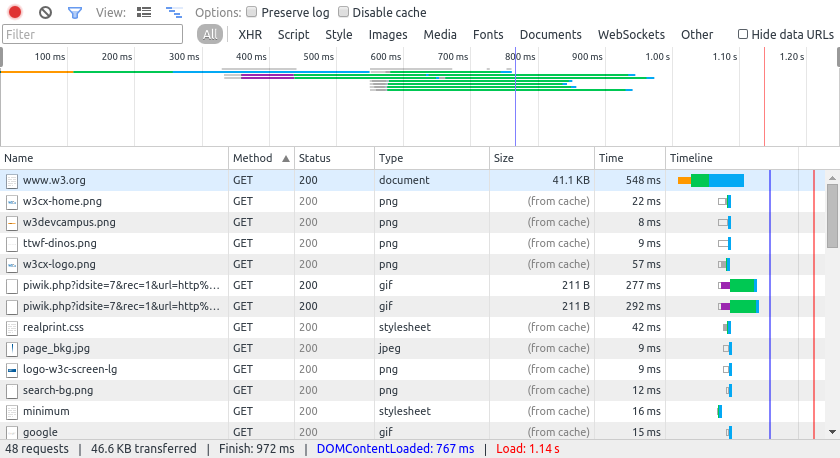
\includegraphics[width=\linewidth]{http_requests}
	\caption{Google Developer Tools window showing HTTP Requests\label{http_requests}}	
\end{figure}

In the above example only the GET HTTP method is used, because the client only requests data from the server, without
sending any data itself. If the client needs to send data to the server, such as form data, or a file, it would still
initiate the connection (the server cannot make requests, only respond, another consequence of statelessness), using
the POST method. While this approach is suitable for a passive, document-based web, where interaction is limited to
jumping from document to document, the web has quickly evolved into an application-based model, where full UIs take
place in the browser space, requiring data be constantly sent back and forth between client and server, in realtime.
This project is one such application.\\

The only way to do this with standard HTTP is periodic polling, which entails large server and network loads. Some
stopgap solutions exist to minimize this overhead, most relevant of which is the Comet web application model. Comet is
based on the concept of long-polling: effectively ``hanging'' the server response until the requested data is
available, and calling another request once the data is received. This approach  still causes increased server loads
but allows some semblance of real-time data transmission. The possibility to use only one connection, as seen in the
previous example was another improvement that became standard in HTTP 1.1. With the HTTP/2 Standard (published in May
2015), the server is allowed to effectively ``push'' data to clients by queuing up more responses than received
requests. However, none of these modifications and hacks are a complete, elegant solution to the problem, given that
HTTP was never intended to be a real-time protocol.\\

That is why other technologies have taken over this new realm of interactivity, providing much more than the ``big,
virtual documentation system in the sky'' \cite{bernerslee09} envisioned by Berners-Lee more than 25 years ago. Some
of them are key parts of this project, as the following sections describe. Still, HTTP remains the initiator for all
these other technologies to function. As of today, any web page you open, no matter how complex the code served in
javascript or flash or any other plug-in still begins with a simple GET request and response.
\section{HTML} \label{HTML}
HTML (Hypertext Markup Language) is the language in which web pages are written. It was created in 1989 by Tim
Berners-Lee as part of his WorldWideWeb, a set of documents linked between each other on a network using the Internet
protocol. It was initially based on SGML (Standard Generalized Markup Language) a document markup language released in
1986 as an ISO Standard (ISO 8879:1986 -- Information processing -- Text and office systems), which was itself derived
from GML (both an acronym for Generalized Markup Language and for Goldfarb, Mosher, Lorie, the last names of its
developers), developed by IBM in 1969.\\

Markup languages in general existed before digital media and still exist in paper based documentation (blue/red
annotations used by editors because lithography/photography/xerography did not capture these colors, the engineering
code for editing documents red = add, blue = delete, green = comment, and many others). In general, markup is a way to
add information regarding the document's structure, presentation, state of development, comments, author, date,
copyright, etc. in a way that is distinguishable from the content of the document. For digital media, it also needs to
be machine-readable, which simply means that a computer must be able to parse this data to extract information. There
are basically two ways of doing this:
\begin{enumerate}
	\item Procedural Markup: A source text is written with instructions for a processing program (equivalent to a
  compiler) to construct the final document. A good example of this method is \TeX, the typesetting system underlying
  the \LaTeX\ macro language (which is itself a mixture of procedural and declarative markup), used to write this
  document.
	\begin{figure}[ht]
    \subfloat[Procedural Source (\LaTeX)]{{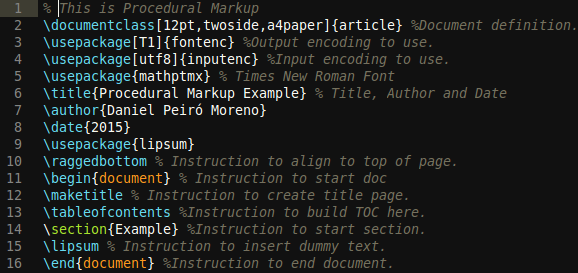
\includegraphics[width=\linewidth/2]{html_procedural_in}}}
    \subfloat[Procedural Output (PDF)]{{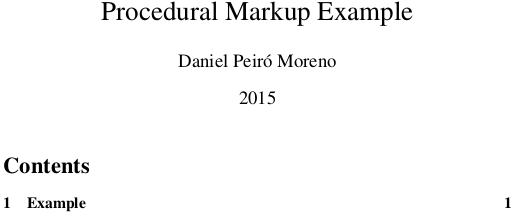
\includegraphics[width=\linewidth/2]{html_procedural_out}}}
    \caption{Procedural Markup Example}
	\end{figure}
	\item Declarative or Descriptive Markup: The content of the text is labeled or ``tagged'' with the markup, without
  giving any instructions on how to process these labels. HTML (especially before HTML5) and XML are clear examples of
  this method.
	\begin{figure}[ht]
    \subfloat[Declarative Input (HTML5)]{{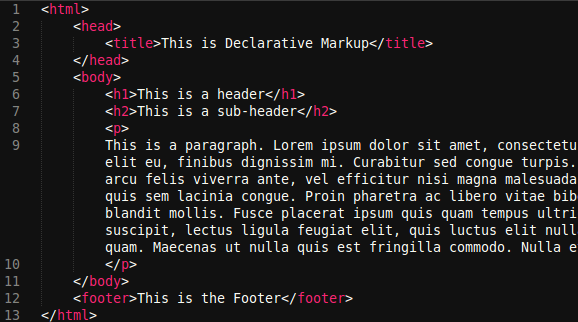
\includegraphics[width=\linewidth/2]{html_declarative_in}}}
    \subfloat[Declarative Output (Google Chrome)]{{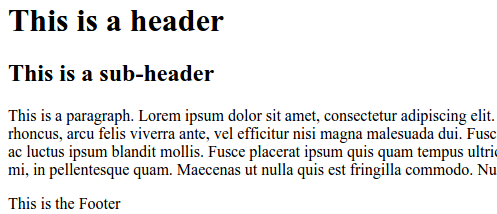
\includegraphics[width=\linewidth/2]{html_declarative_out}}}
    \caption{Declarative Markup Example}
	\end{figure}
\end{enumerate}
HTML and its precursor SGML are essentially declarative markup languages. The main advantage of declarative markup,
and more generally the declarative programming paradigm is the decoupling of the intended result and the processing
required to achieve it. This has been crucial for HTML to be able to evolve and adapt dynamically over decades of
technological innovation. The computers and programs used in 1989 have very little in common with those used today in
many cases. A markup language designed to be ubiquitous, read on an ever changing array of software and hardware
platforms and permanently backwards compatible, where a web page designed in 1991 is just as valid as one designed
using the last specification, has to be as procedurally oblivious as possible.\\

The basic HTML markup unit is the tag. A tag is simply a keyword surrounded by brackets. HTML tags usually come in
pairs, an opening tag and a closing tag (designated adding a forward slash after the first bracket), that give markup
information on the enclosed content:
\begin{figure}[h]
\centering
\RecustomVerbatimEnvironment{Verbatim}{BVerbatim}{}
\begin{minted}[breaklines,fontsize=\footnotesize]{html}
<!--This is a comment-->
<h1>This is a heading</h1>
<p>This is a paragraph</p>
<div>This is a section</div>
<table>
  <tr>
    <th>Table Header Cell 1</th>
    <th>Table Header Cell 2</th> 
  </tr>
  <tr>
    <td>Table Cell 1</td>
    <td>Table Cell 2</td> 
  </tr>
</table>
<ul>
  <li>List Element 1</li>
  <li>List Element 2</li>
  <li>List Element 3</li>
</ul>
<a href="http://www.w3.org">This text links to W3C Web Page</a>
\end{minted}
\caption{Declarative HTML Tags}
\end{figure}\\
All of the tags in the above example are purely declarative. They state what the enclosed text is, leaving it up to
the parser how to obtain the desired result. To extend markup within a tag, attributes are added and given a value. For 
example, the href attribute in the <a> hyper link tag above points to the URL the browser will go to when the text is 
clicked. As the web evolved since it's inception, adding interactivity to documents, more tags were added to HTML that 
weren't so clearly declarative and had a behavioral component, as well as semantic attributes:\\
\begin{figure}[h]
\centering
\RecustomVerbatimEnvironment{Verbatim}{BVerbatim}{}
\begin{minted}[breaklines,fontsize=\footnotesize]{html}
<form action="" method="">
  <input type="text" name="input1"><br>
  <input type="text" name="input2"><br>
  <input type="button" value="value0" onclick="">
  <input type="checkbox" name="input3" value="value1">
  <input type="radio" name="input4" value="value2"><br>
  <input type="radio" name="input5" value="value3">
  <input type="submit" value="Submit">
</form>
\end{minted}
\caption{Behavioral HTML Tags}
\end{figure}\\
These behavioral tags (and many others) were a response to the demand for a more interactive web, not only composed of
linked documents, but of applications implementing business logic and data transactions. They were added by web
browser developers independently, and in consequence were incompatible with other software as well as poorly
documented. In 1994, Tim Berners-Lee created the W3C (World Wide Web Consortium) to solve this problem, attempting to
achieve consensus between browser developers developing standard versions of HTML. This helped HTML remain relatively
simple and consistently usable across browsers. The W3C also attempted to standardize the way browsers parsed HTML,
which initially was very lenient to errors. The repercussions of these attempts will be discussed in section
\ref{HTML5}, specifically related to HTML5, as they indirectly led to the standard.\\

HTML tags can be nested, with the outer tags being called parent tags, and tags enclosed by others called children.
This nested structure, which can also be seen as a tree structure is called the Document Object Model or DOM for short.
This model represents all of the objects included in the document in nodes, with parent nodes encapsulating child nodes,
and one root node that encapsulates all of them. To create the DOM, different browsers use different methods, called
layout engines that parse the HTML to create the DOM Tree. This tree serves only the purpose of correctly representing
nested content on a page, where static web pages are concerned. However, the DOM is crucial for dynamic web pages, as it
provides external controllers, such as JavaScript a model to interact with (see section \ref{JavaScript} on JavaScript).\\

In this project there is just one HTML document (albeit one composed of more than 500 lines of markup) and therefore only
one DOM Tree, as it implements the ``Single Page Application'' user interface paradigm as a means to make the user
experience more fluid and similar to that of a native program. The structure of the page, which is decidedly non-
declarative as a whole, is nonetheless defined using almost exclusively declarative tags. Only multimedia is truly
generated dynamically on the page, with everything else being declared statically, with the caveat of being bi-
directionally bound to a model which in turn is dynamically changed (see section \ref{AngularJS} on AngularJS).\\

The declarative markup method has many advantages as shown: simplicity, portability, light-weight parsing... But it's
main flaw remains that it lacks the ability to create complex structures, interactive structures, and dynamic
structures. Declarative markup is distinctly static in nature: once parsed, the content is presented and remains the
way it was declared (at least in purely declarative tags). This is not a flaw inherent to its design, as it was designed
to markup documents, but one created through the evolution of the web. HTML as a language has itself evolved, blurring
the lines of declarative and behavioral markup (see section \ref{HTML5} on HTML5 for more), but for interactivity and
complexity to truly flourish, markup as a whole just isn't enough. As early as 1995, it became evident that the web
needed a programming language. That language was JavaScript.
\section{JavaScript} \label{JavaScript}
\begin{figure}[h]
\centering
\includesvg[width=1.1\linewidth/4]{./img/javascript}
\caption{JavaScript Badge}
\end{figure}
JavaScript is a programming language. The most common use for JavaScript is running scripts alongside web pages, making
them dynamic and interactive in ways HTML alone cannot. JavaScript was created by Netscape, an early web browser vendor
and developer in 1994, as part of its Netscape Navigator browser. Originally named Mocha, then LiveScript and finally
JavaScript (not because it is related to the Sun developed language, but as an attempt by its creators to use the
popularity of Java for marketing reasons). It was initially conceived as a ``glue'' programming language to be used by
web designers with little programming knowledge or experience to include Java (considered a more ``serious'' and powerful
language at the time) applets in their pages without necessarily knowing anything about Java programming. It quickly
evolved beyond that, becoming a programming language in it's own right. After Microsoft included it in Internet Explorer
3.0 in 1996 (as JScript, to add to the naming confusion), Netscape sought to standardize the language through the ECMA
standards organization, eventually leading to ECMAScript, the current technical name of the language (used only in
standard versions). The current standard is ECMAScript 5 originally released in 2009, while ECMAScript 6 will be released
sometime in 2015. Although JavaScript is mainly used client-side even today, it was originally conceived to also run
server-side. This concept was widely ignored during the early days of the web, focusing on client-side dynamic scripting,
while using other languages (PHP, CGI, Perl, etc.) on the server-side. The late 2000s and early 2010s have seen a
resurgence of the idea of server-side JavaScript allowing full-stack (front-end to back-end in JavaScript) applications,
like this project, to exist. This will be covered in section \ref{TheMEANStack} on the MEAN Stack.\\

The formal classification and description of JavaScript as a language is beyond the scope of this overview, so it won't
be discussed here. Suffice it to say that it's a prototype-based, dynamically-typed scripting language, which allows it
to implement multiple programming paradigms (imperative, functional and object oriented), sacrificing performance (as do
all dynamic languages) and formal elegance for a high level of abstraction, flexibility and dynamic execution.\\

The key aspect of client-side JavaScript is that runs in the browser, dynamically modifying the HTML document. A
JavaScript script is included in an HTML document simply by using the script tag:
\begin{figure}[h]
\centering
\RecustomVerbatimEnvironment{Verbatim}{BVerbatim}{}
\begin{minted}{html}
<script type="text/javascript" src="examplescript.js"></script>
\end{minted}
\end{figure}

As seen in section \ref{HTTP} on HTTP, this tag will trigger a HTTP GET request to the server for the text file
``examplescript.js'', that the browser will parse as JavaScript, and dynamically execute, with total transparency
from the users point of view. This script could, in a typical early web use-case, modify the web page dynamically,
without necessarily triggering new HTTP requests to the server, given that once the script is served, it is running
independently on the client system. For modifications to be possible, a machine-readable model of the web pages' content
and markup is required. The DOM (Document Object Model, see section \ref{HTML} on HTML) is the convention used to model
the page, and is kept in memory by the JavaScript Engine as the global ``state'' of the page. Scripts can then get
information from the model, as well as control and modify the model. The browser will then refresh the representation of
the page, following a classic Model (DOM), View (Browser window), Controller (JavaScript scripts) paradigm.\\

This use-case, while still the most extended use for JavaScript has given way in the last decade and a half to a much
more behavior-centric use, where JavaScript no longer is an add-on or enhancement to HTML, as much as a fundamental part
of how we understand web pages, to the point where the latest standard in HTML includes many tags that are simply useless
without JavaScript to provide the behavior behind them. This demand for interactivity has also led to some pages that are
sloppy when it comes to separating behavior and structure of a web application, tending to use JavaScript for everything,
even when HTMLs declarative approach is more appropriate for a given use-case, simply because JavaScript is more
``comfortable'' from a programmers perspective. This brings with it code maintainability, elegance and performance issues
if not handled correctly. To help maintain declarative and behavioral code separate, and use each one when appropriate,
JavaScript frameworks such as AngularJS have appeared, allowing highly dynamic, complex, single-page web applications to
keep a Model-View-Controller paradigm. This framework, as part of the MEAN Stack, is used in this project (see section
\ref{AngularJS} on AngularJS).

JavaScript essentially provides behavior, interactivity and dynamism to otherwise static HTML. Other methods of adding
these traits to web pages exist and some remain popular today. Java Applets run in a JVM (Java Virtual Machine) once
executed from an HTML document. Adobe Flash (previously Macromedia Shockwave Flash) allows full animations, video and
audio to play embedded inside of a web page. Microsoft Silverlight (now deprecated) served a similar purpose as Flash.
All of these technologies had the major flaw of not integrating with HTML as much as substituting it, or embedding a
``black-box'' in it. This impacts platform compatibility, performance, and accessibility (without going in to the
problems that arise from proprietary technologies). Of the previous, only Flash remains relevant today, mainly as a means
to provide multimedia content, where the HTML standard is considerably lagging behind. But even then, Flash today is
either incompatible or unsupported on all major mobile platforms, and is quickly being substituted with HTML5 by
multimedia providers (Youtube, for example, now defaults to an HTML5 player as opposed to Flash). JavaScript on the other
hand has been consistently relevant since it's inception and continues to grow in importance as a web technology,
expanding to the back-end, and becoming inextricably embedded in the latest HTML standards. This is precisely because it
doesn't try to substitute or deprecate HTML, but complements it by adding behavior to structure, while allowing both to
remain separate.
\section{CSS} \label{CSS}
\begin{figure}[h]
\centering
\includesvg[width=\linewidth/4]{./img/css3}
\caption{CSS3 Badge}
\end{figure}
HTML provides structure to web documents. JavaScript adds behavior, turning documents into applications. CSS (Cascading
Style Sheets) adds style, giving the document renderer instructions on the presentation of the structure created with HTML.
This gives documents and applications, which have no inherent visual representation, a distinct style, as chosen by the
designer, not by the renderer. CSS was created by Håkon Wium Lie and Bert Bos in 1994. It was originally named Cascading
HTML Style Sheets (CHSS), as it was aimed exclusively at HTML styling. The H was soon dropped from the name, as the authors
wanted CSS to be applicable to other markup languages. CSS, like HTML wasn't the first language of it's kind. Style sheet
languages like DSSSL (Document Style Semantics and Specification Language) or FOSI (Formatted Output Specification
Instance) were created for HTMLs precursor, SGML (see section \ref{HTML}). However, these languages didn't allow for style
sheets to be separated from the document, and were therefore unsuitable for the nature of the web, while also being deemed
too complex. CSS has been standardized by the W3C since it's creation, producing three main recommendations:
CSS1 in 1996, CSS2 in 1998, and CSS3 which was divided into modules for different aspects of the language, some of which
have already been finished in the last few years, others still evolving. CSS4 development has begun on completed modules,
but will not be extensively worked on until CSS3 is finalized.\\

Before CSS, HTML either was devoid of any presentational specifications (leaving all styling to the default specified by
the renderer, making all web pages quite simple and unappealing) or had to be styled from within HTML. This was done using
presentational tags, which remained part of HTML standard until HTML4 (see figure \ref{presentational_tags}).\\
\begin{figure}[h]
\centering
\RecustomVerbatimEnvironment{Verbatim}{BVerbatim}{}
\begin{minted}{html}
<h1>
  <font size="3" color="red">This is a heading</font>
</h1>
<body background="bgimage.jpg"><!--Use image as background-->
<strike>This text is strikethrough.</strike>
<img src="exampleimage.png" border="5"><!--Image with 5px border-->
<center>This text will be center-aligned.</center>
</body>
\end{minted}
\caption{Deprecated Presentational Tags \label{presentational_tags}}
\end{figure}

This presented the problem of mixing declarative, structural markup with styling, making the structure much less clear to
the editor, which in turn led to error-prone design, while still being a limited solution, given the amount of tags needed
to be kept in check, if there was to be any structure to the language.\\

CSS allows, similarly to how JavaScript does with behavioral components, the addition of style without substituting
structure while keeping a separate environment for each. With CSS, the only tag necessary is the style tag, or if included
from another file, the link tag:
\begin{figure}[h]
\centering
\RecustomVerbatimEnvironment{Verbatim}{BVerbatim}{}
\begin{minted}{html}
<head>
<link rel="stylesheet" type="text/css" href="stylesheet.css">
</head>

<!--OR-->

<style>
h1 {
font-size: 3px;
color:red;
}
</style>
\end{minted}
\caption{Linking or including CSS in HTML}
\end{figure}
This separates the structure and the presentation of the web page neatly, allowing both to remain clear, readable and
maintainable.\\

The main styling unit of CSS is the rule. A rule is composed of selector and a declaration block. A selector specifies the
target of a set of style specifications (declarations) that follow in the declaration block. In the previous example, there
is only one rule, with selector h1 and declarations font-size and color. This rule will target all h1 tags present in the
document and apply the declarations inside the declaration block to the content of the tag. There are a wide range of
selectors available, from the simplest like the wild-card, *, that targets all elements, to complex, composite selectors
that target elements with certain attribute values (particularly useful is the ".class" selector that targets all elements
with a certain class attribute value), pseudo-selectors that target elements under certain circumstances (``:hover''
targets elements with the mouse over them), etc. which allow complete control over the presentation of web pages.\\

While rules provide granular presentational control over the web page, as a standalone, they would be cumbersome at best
and impossible to implement at worst were it not for cascading. Cascading allows the definition of a hierarchical structure
in the way rules are applied, where rules with a higher priority override lower priority rules. There are several
priority definitions (for example, in line style tags prevail over included stylesheets), but the most important is
selector specificity. If an element fits the target for two or more selectors, the one with the highest specificity will
prevail, if that rule defines a conflicting declaration. For example:
\begin{figure}[h]
\centering
\RecustomVerbatimEnvironment{Verbatim}{BVerbatim}{}
\begin{minted}{css}
/* Applies to all elements */
* {
  color: green;
  text-align: center;
}

/*
  Applies to h1 elements.
  Overrides color from *,
  keeping text-align: center.
*/
h1 {
font-size: 3px;
color:red;
}

/*
  Applies to p elements nested in div elements.
  Overrides both * declarations.
*/
div > p {
  color: blue;
  text-align: right;
}

/*
  All other elements will apply *,
  without need for more rules.
*/
\end{minted}
\caption{Cascading CSS Specificity.}
\end{figure}
\\(Note: Use of * selector is somewhat inefficient and inelegant, used here for illustration purposes).\\

Without this feature, it would be necessary to specify styles for each type of element, or leave some up to the renderer.
This, as previously stated would be tedious for document based pages, and near impossible for applications.\\

This project implements the ``Single Page Application'' user interface pattern, and therefore only one style sheet is used.
In websites with multiple web pages, there's normally one root style sheet that defines the general presentation of the
site, common to all pages, and each page may have it's own particular style sheet for more specific presentation
specification. This allows for neat compartmentalization of styling, which benefits maintainability, future development and
documentation.\\

Some of the more modern modules of CSS3 used in this project (media queries and transitions) will be discussed in section
\ref{HTML5} on HTML5. Even though CSS3 is technically a separate entity and W3C standard, it is most certainly part of the
wider definition of HTML5 as "the cornerstone for modern web applications"\cite{w3c11}.
\section{HTML5} \label{HTML5}
\begin{figure}[h]
\centering
\includesvg[width=1.4\linewidth/4]{./img/html5}
\caption{HTML5 Badge}
\end{figure}
HTML5 is the latest version of the HTML (see \ref{HTML} on HTML in general) Specification Recommendation developed and
published by the W3C (in its final form, development started outside the Consortium) released the 28th of October, 2014.
The significance of this date is somewhat diminished given that HTML5 has been in development since 2004, and many of the
APIs (Application Programming Interface) it specifies have been implemented in browsers preceding the formal release date,
in many cases years in advance.\\

The fundamental change between HTML5 and previous versions of HTML is the shift to a Web Application model from the
original Web Document model. This change came as a response to the direction the W3C had taken after the publication of
HTML 4.0 in 1997, which was much more conservative. At that time, the W3C was very concerned with broken HTML: it is
assumed (including by the W3C\cite{w3cwebquality02}) that 99\% of web pages are not valid HTML. This is made possible by
the lenient error handling methods used by browser HTML parsers. When a browser finds an error in an HTML document 
(incorrect tag spelling, unclosed tags, missing brackets, incorrect nesting order etc.), instead of stopping and not 
rendering the page, it works around the error, displaying the page as well as it can. This allows for web pages to have 
minor errors that do not alter the overall display of the page, remaining usable for most users, and more importantly, 
allowing anybody that has a basic knowledge of the language to write a web page without having to become an expert, 
effectively making HTML a much more accessible and universal language. The downside to this is inconsistency, which is 
what concerned the W3C: What methods are used in this lenient error handling? Are they to be standard? Proprietary? Which 
errors are permissible? Are future browsers going to be able to read invalid pages which were parsed with undocumented 
error handling methods? All these valid concerns lead the W3C to a drastic decision: draconian error handling.\\


The W3C established that the next HTML standard, called XHTML 1.0, would have to be well-formed XML (eXstensible Markup
Language, a profile of SGML) to be rendered. This, technicalities aside, meant that all documents that wanted to be valid
markup under the new specification, would need to have no errors for browsers to render them. If not, the page would not
render and an error message would be presented to the user. Even for a single mistyped tag. This also rendered all
previous, error laden web pages obsolete in the eyes of the W3C.\\

As discussed in previous sections, attempts to deprecate existing HTML or substitute it with something new, have been in
general unsuccessful. XHTML was no exception. Given that the benefits of upgrading were few, and barely apparent for the
general public, web creators didn't make the jump from HTML 4.0. XHTML 1.0 allowed, through a transitional loophole, the
possibility of declaring the document as XHTML while keeping lenient error handling from HTML 4.0. Even then, adoption was
slow, but when XHTML 1.1 closed this loophole, it sealed its fate as a failed ``upgrade''.\\

After XHTML, the W3C was at an impasse of sorts. It had spent years on the development of XHTML, which had a very low
adoption rate and the power of home computing was sky rocketing, leading to demands for web applications instead of
documents to increase immensely. In 2004, it held a workshop (The W3C Workshop on Web Applications and Compound Documents
\cite{w3c04}) to define the future of web applications. Many manufacturers and interest groups proposed that a series of
mid-level APIs should be developed as extensions to HTML and CSS for use in Web Applications as opposed to fully fledged OS
-Level APIs. This meant leaning toward in-browser solutions as opposed to ``black-box'' plug-in software (such as Java
Applets or Flash). This proposal was rejected (see Workshop Summary straw poll topic no. 3 in \cite{w3c04}), and led to a
group of the proposers to create a work group outside the W3C, the WHAT Working Group (Web Hypertext Applications
Technology Working Group). This group went in the opposite direction the W3C did to solve HTMLs error handling problems
and the evolution of the web. Instead of dropping error handling altogether, like XHTML did, the WHAT group decided it
would specify and document the way lenient error handling works, so that it would no longer rely on proprietary, poorly
documented solutions that made future proofing and maintaining compatibility among different browsers virtually
impossible. This wasn't as easy as the XHTML solution, in fact it took 5 years to complete, but it allowed full backwards
compatibility for older pages, a crucial aspect of evolving the web, as seen in previous sections. For Web Applications,
the WHAT group turned away from plug-ins, and started work on three of the most important multimedia APIs present in
HTML5: Canvas (direct-mode drawing) and native Audio/Video support.\\

In 2006, Tim Berners-Lee announced that the W3C would start working with the WHAT WG to evolve the web. The new HTML
Specification that would come from this new group, would be called HTML5.\\

HTML5 introduced a long list of new features to HTML, most of them directed at Web Application Development:
\begin{itemize}
  \item \textbf{Canvas Element}: Direct Mode 2D Drawing. Essentially allowing for fully native animations.
  \item \textbf{Audio and Video Element}: Native multimedia support, effectively deprecating flash.
  \item \textbf{Geolocation}: Allows sharing the clients location with the application seamlessly.
  \item \textbf{Local Storage}: Allows the application to store data on the clients computer.
  \item \textbf{Offline Web Applications}: Once downloaded, the application can run without being connected to the Internet.
  \item \textbf{WebSockets}: Full duplex communication between client and server, in one TCP connection. (Now a separate specification)
  \item \textbf{Web Workers}: JavaScript running in the background, taking full advantage of the client CPUs power for heavy tasks.
\end{itemize}
While others were much needed upgrades and deprecations of HTML 4.0 features, such as the addition of a wealth of new
controls to forms and semantic tags, as well as the removal of presentational tags altogether. Only the features used in
this project will be discussed briefly further.
\subsection{HTML5 Semantics}
\begin{figure}[h]
\centering
\includesvg[width=1.4\linewidth/8]{./img/html5_semantics}
\caption{HTML5 Semantics Badge}
\end{figure}
HTML5 Semantics are used to more clearly and succinctly define the elements content. This improves the readability of the
markup and allows browsers to make better accessibility tools. It makes the markup easier to read by eliminating
unnecessary text:\\

\begin{figure}[h]
\centering
\RecustomVerbatimEnvironment{Verbatim}{BVerbatim}{}
\begin{minted}{html}
<!--In XHTML 1.0-->
<!DOCTYPE html
          PUBLIC "-//W3C//DTD XHTML 1.0 Strict//EN"
          "http://www.w3.org/TR/xhtml1/DTD/xhtml1-strict.dtd">
<html xmlns="http://www.w3.org/1999/xhtml"
      lang="en"
      xml:lang="en">
</html>
<!--In HTML5-->
<!DOCTYPE html>
<html></html>
\end{minted}
\caption{HTML5 Semantics: Text Usage Comparison}
\end{figure}
And by giving names to typical web page components:\\

\begin{figure}[h]
\begin{center}
  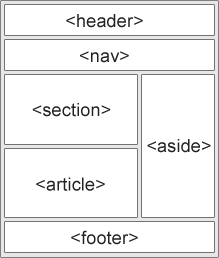
\includegraphics[width=\linewidth/3]{html5_layout}
  \end{center}
  \caption{HTML5 Semantics: Typical Page Layout. Source: \href{http://www.w3schools.com/html/html5_semantic_elements.asp}{
  W3Schools}.}
\end{figure}
This allows web browsers to better understand what the content is declared as, and choose to present it in different ways (
for example, a page with an article and a header might be presented differently on a mobile browser to enhance the reading 
experience), and allows for accessibility features such as text-to-speech to present the content in a fitting manner.\\

In this project, the page is written using HTML5 semantics, reducing the amount of superfluous text, making it easier to
read (taking into account the complexity of the liquid layout). It also uses the header and footer tags to frame the
controls, using the header as the title of the page, and the footer to include copyright acknowledgments and references.
\begin{figure}[h]
\begin{center}
  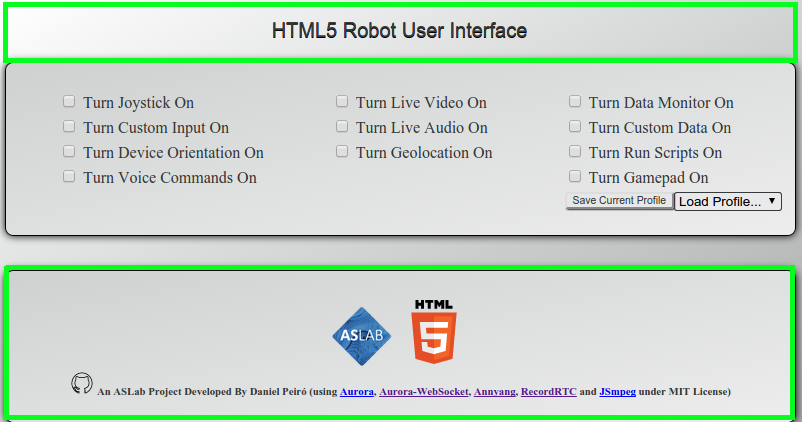
\includegraphics[width=\linewidth]{html5_headerfooter}
  \end{center}
  \caption{HTML5 Semantics: Use of Header and Footer (Marked in green) in HRUI}
\end{figure}
\subsection{HTML5 Canvas Element} \label{html5canvaselement}
\begin{figure}[h]
\centering
\includesvg[width=1.4\linewidth/8]{./img/html5_canvas}
\caption{HTML5 Graphics Badge}
\end{figure}
The Canvas element is, in the simplest terms possible, a rectangle in a web page in which a JavaScript script can draw
anything. It allows things as simple as drawing a line with the cursor, to full fledged game graphics, and requires
nothing but a canvas element (\mintinline{html}{<canvas></canvas>}) and access from JavaScript to said element. By
changing the drawing at a fast enough frequency, animation becomes trivial.\\

In this project, the canvas element is used for three of its modules. It's used to create virtual joysticks for the user
to control dynamically with the mouse or using a touch interface (see section \ref{joystick} on the Joystick input module).\\

\begin{figure}[h]
\begin{center}
  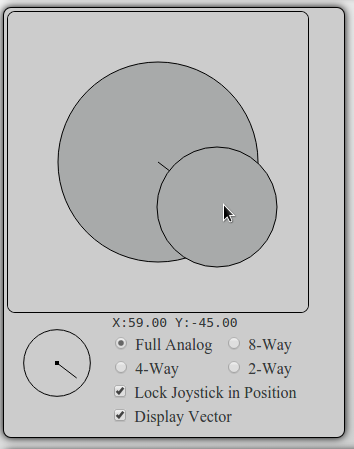
\includegraphics[width=\linewidth/3]{joystick}
  \end{center}
  \caption{HTML5 Canvas: Joystick in HRUI. (2 Canvas Elements: Joystick and Vector)}
\end{figure}
It's used for the live video feed, using JSMpeg, a MPEG1 decoder written in JavaScript (see section \ref{livevideo} on the
Live Video module). It's also used for the dynamic obstacle map in the data monitor module (see section \ref{datamonitor}),
which can be generated from the server, uploaded by the user or can even be drawn on the fly with the cursor or touch
interfaces (see figure \ref{html5_map}).\\

\begin{figure}[h]
\begin{center}
  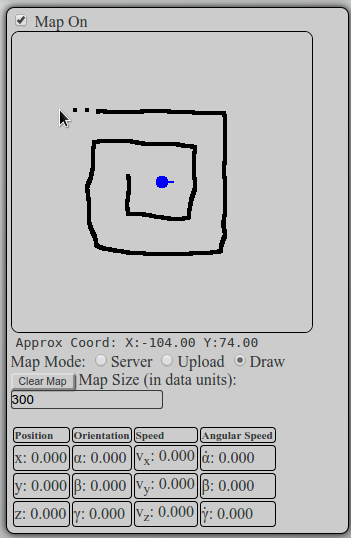
\includegraphics[width=\linewidth/3]{html5_map}
  \end{center}
  \caption{HTML5 Canvas: Map in HRUI. (Black: Drawn Obstacles. Blue: Robot Pos.)\label{html5_map}}
\end{figure}
The Canvas API allows for essentially any sort of content to appear on a website natively without the need for flash, which
was the go-to resource for animation previously. This amounts to a big leap in graphics and animation versatility for HTML.\\

\subsection{HTML5 WebSockets} \label{html5websockets}
\begin{figure}[h]
\centering
\includesvg[width=1.4\linewidth/8]{./img/html5_connectivity}
\caption{HTML5 Connectivity Badge}
\end{figure}
WebSockets allow for full-duplex communication between server and client using one TCP connection. As its name implies it's
most easily described as an implementation of TCP/IP Sockets for the web. It allows for fully bidirectional communication,
using only one HTTP request (see section \ref{HTTP} on HTTP), that is upgraded to a WebSocket connection. This HTTP handshake
is important, as it allows for a graceful backwards compatibility, using the same technology as standard web pages.\\

WebSockets are essential for this project. As a real-time application, data needs to move to and from the client and the
server constantly to relay instructions from the controls to the back-end, and update output data to the front-end.
Furthermore, to live stream media from the server to clients, WebSockets are used, providing minimal latency. Without
WebSockets this project would be almost impossible to achieve, with any measure of success.\\

The WebSockets API in HRUI is implemented in two forms: raw and through the Socket.IO framework. The raw form creates and uses
WebSockets through direct calls to the API and is used for media streaming. The Socket.IO framework adds a layer of
abstraction to WebSockets, by creating an event-based model. An event is a message that is broadcast by an emitter and
captured by a listener. The emitter and listener are the server and client, and vice versa. An event carries attached to it a
JavaScript object which will be received by the listener. The programmer creates these asynchronous events on either the
server or the client, establishing the behavior of the listener. For example: Every 50 ms the back-end wants to send the front-
end an update on the value of X in the robots position. With Socket.IO (after setup) the code would be:\\

\begin{figure}[h]
\centering
\RecustomVerbatimEnvironment{Verbatim}{BVerbatim}{}
\begin{minted}[fontsize=\footnotesize]{javascript}
//On the Server side:
//[...](setup and surrounding code omitted for clarity)
var x = 10; //value of robot X coordinate (defined here for brevity)

socket.emit("UPDATE_X", x);
//emit an event with message UPDATE_X and data x (value: 10)

//On the Client side:
//[...](setup and surrounding code omitted for clarity)
socket.on("UPDATE_X", function(received_x) {
              console.log(received_x);
            };
//listen for an event with message UPDATE_X
//and print the value of the data received to the console.
\end{minted}
\caption{HTML5 WebSockets: Socket.IO Event Example}
\end{figure}
This added layer of abstraction makes using WebSockets very simple, needing only to define when and where in the code events
are generated and adding listeners for these events. It also makes code much easier to understand, and much more structured,
closer to the business logic and separated from low level serializing and underlying connections.
\subsection{HTML5 Device Access}
\begin{figure}[h]
\centering
\includesvg[width=1.4\linewidth/8]{./img/html5_device_access}
\caption{HTML5 Device Access Badge}
\end{figure}
HTML5 Device Access allows the web application to use the hardware of the machine the browser is running on. This means
anything from microphones and cameras to accelerometers and GPS data.\\

HRUI makes full use of three of these APIs:\\

\begin{itemize}
  \item \textbf{Microphone}: The Voice Command module (see section \ref{voicecommands}) uses device access to receive audio
  from the users microphone, which is then recognized (using Annyang) into commands which are sent to the server for use (see
  figure \ref{html5_voice}). It also uses the WebRTC API to enable an alternative in non-chromium browsers that don't have the
  speech recognition API, by recording a 5 second audio clip that is sent as a .wav file to the server. WebRTC started out as
  part of HTML5 but has spun out into its own specification, that allows for peer-to-peer server-less audio and video sharing,
  among many other multimedia uses which are outside of this reports scope, since they're not used in this project.

  \begin{figure}[h]
    \begin{center}
      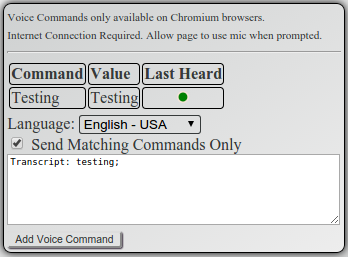
\includegraphics[width=\linewidth/2]{html5_voice}
    \end{center}
    \caption{HTML5 Device Access: Voice Commands in HRUI.\label{html5_voice}}
  \end{figure}
  \item \textbf{Device Orientation}: The Device Orientation module (see section \ref{deviceorientation}) gets the orientation,
   velocity and acceleration from the device (if available) and sends it to the server for use (see figure 

  \ref{html5_orientation})
  \begin{figure}[h]
    \begin{center}
      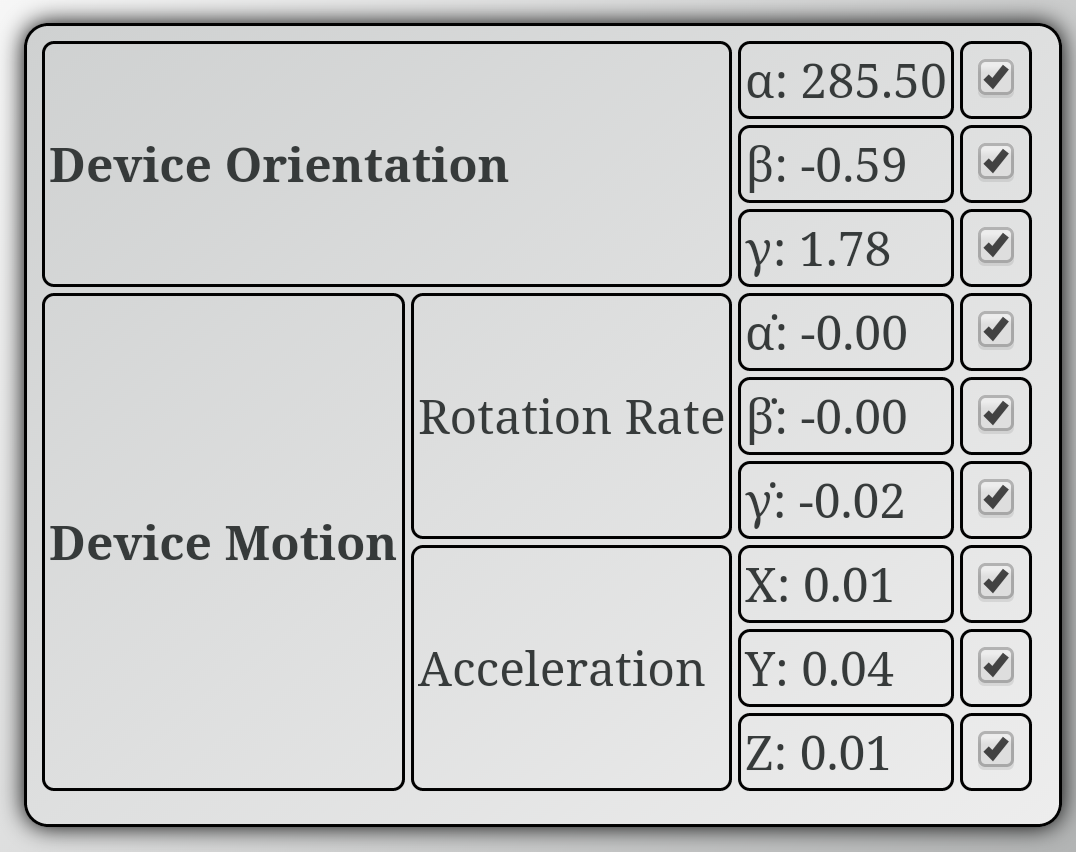
\includegraphics[width=\linewidth/2]{deviceorientation}
    \end{center}
    \caption{HTML5 Device Access: Device Orientation in HRUI.\label{html5_orientation}}
  \end{figure}
  \item \textbf{Gamepad}: The Gamepad module (see section \ref{gamepad}) uses the Gamepad API to get the inputs of a gamepad
  connected to the client machine and send them to the server for use. This extends the HRUI web application controls to
  virtually any device that can be connected to a web capable device as an input, allowing for external hardware to function
  seamlessly with this project with little to no integration effort. However, this API is still experimental at the time of
  writing, and support is limited to a few browsers (Chrome and Firefox mainly), with different implementations that require
  tweaking of parameters (mainly the mapping of buttons, which changes from Chrome to Firefox and with the controller in use)
  for consistent usage.
\end{itemize}
\subsection{HTML5 Styling} \label{html5styling}
\begin{figure}[h]
\centering
\includesvg[width=1.4\linewidth/8]{./img/html5_css3}
\caption{HTML5 Styling Badge}
\end{figure}
HTML5 Styling is actually a misnomer, albeit one used by the W3C, because it considers that HTML5 refers to more than just the
latest HTML Recommendation, encompassing several specifications and should be used as an umbrella term to encapsulate all
technologies of the modern web, calling HTML5 "The cornerstone for modern Web applications"\cite{w3c11}. This is cause of some
debate among enthusiasts, but controversy aside, the fact is that HTML5 has no significant styling features (in consonance
with the separation between declarative and presentational discussed in previous sections), relying on the CSS3 (Cascading
Style Sheets, see section \ref{CSS}) specification for innovation in this aspect.\\

In HRUI many new CSS3 features are used to make the application more visually attractive and useful on different devices:\\

\begin{itemize}
  \item \textbf{Media Queries}: One the most useful additions made to CSS3 is the ability to apply styles to different
  viewports (the space where the web page is rendered in a browser) and device types without having to make different versions
  of the site, by using media queries. A media query basically defines a subset of styling rules that apply only to viewports
  that fit a certain criteria, while keeping in place the cascading nature of CSS. This means that by making, for example, a
  media query on the pixel width of the screen, a set of rules will be applied that can drastically change the presentation of
  the page. In HRUI only one media query is made, specifically to target smartphones (truncated for brevity):\\

  \begin{figure}[h]
    \centering
    \RecustomVerbatimEnvironment{Verbatim}{BVerbatim}{}
    \begin{minted}[fontsize=\footnotesize]{css}
      @media only screen and (max-width: 480px) {
          .frame {
              width: 100%;
          }
          #rightColumn, #centerColumn, #leftColumn {
              float: left;
              clear: both;
              width: 98%;
          }
      }
    \end{minted}
    \caption{HTML5 Styling (CSS3): Media Query in HRUI}
  \end{figure}
  Which targets screens under 480 pixels wide and applies the enclosed rules only to those screens. All other styling is
  maintained and applied, through cascading. These rule (and others omitted for brevity) make all modules occupy the whole
  width of the screen, more appropriate for small, touch based devices than the three-column default for computers and
  tablets. The user can then scroll through the modules to use them since including more than one module on a smartphone
  screen at once would clutter the interface and make it virtually unusable. This approach makes a necessary compromise by
  allowing the active visualization of one module at a time, while allowing all modules to run in the background, visible at
  the slide of a finger.
  \begin{figure}[h]
  \captionsetup{justification=centering}
      \begin{center}
        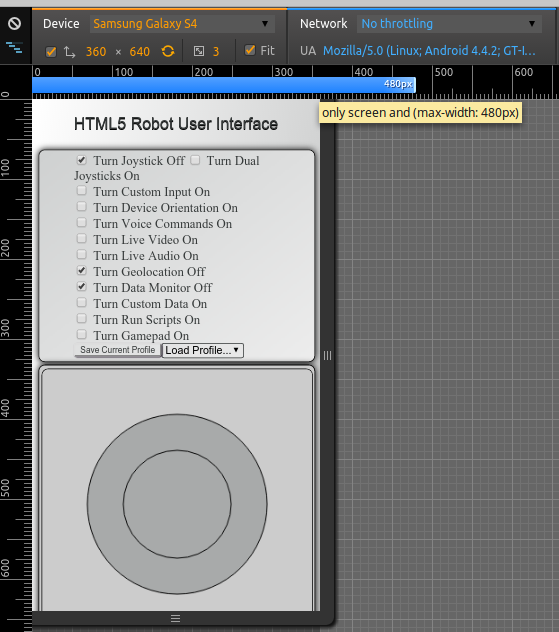
\includegraphics[width=\linewidth/3]{html5_css_mq2}
      \end{center}
      \caption{HTML5 Styling (CSS3): HRUI Smartphone version\\(simulated SGS4 using Chrome Dev Tools. Blue bar marks the
      detected media query)}
  \end{figure}
  \begin{figure}[h]
    \begin{center}
      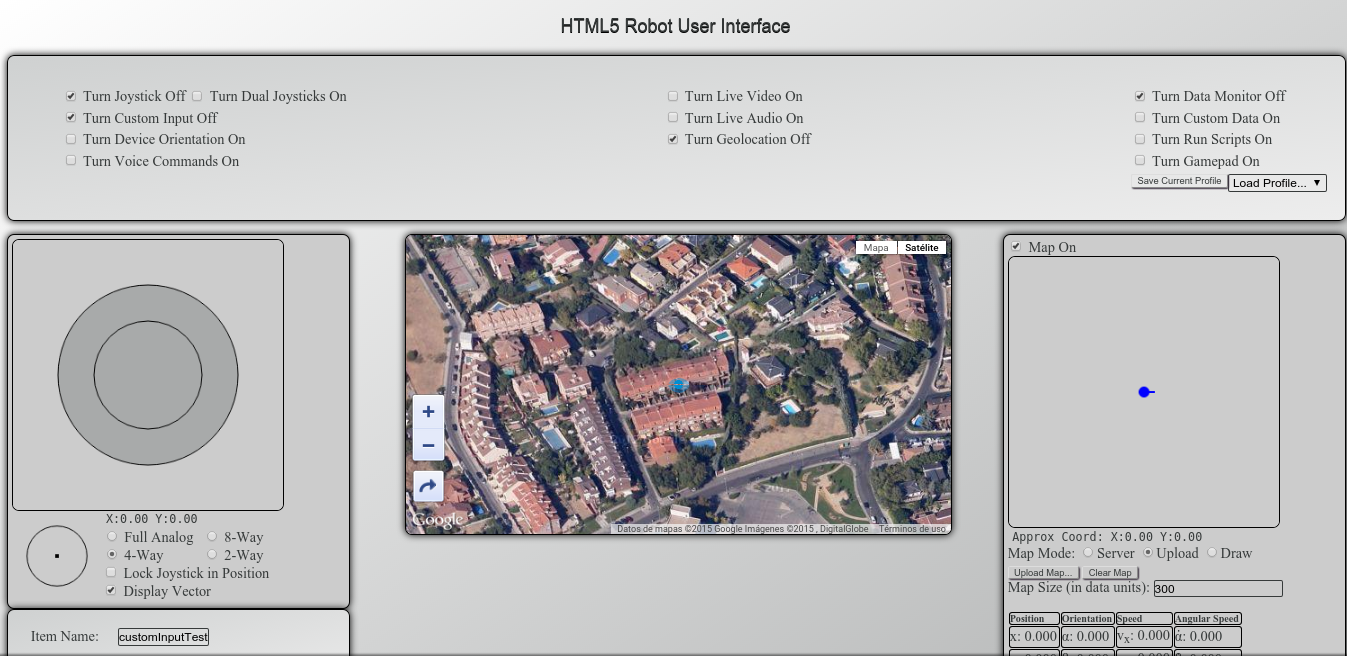
\includegraphics[width=\linewidth/2]{html5_css_mq1}
    \end{center}
    \caption{HTML5 Styling (CSS3): HRUI Laptop version}
  \end{figure}
  \item \textbf{Transitions}: CSS3 Transitions can make the value of element properties change over time, creating an
  attractive visual effect. HRUI uses this feature (combined with AngularJS Animate, see section \ref{AngularJS}) to animate
  module activation and deactivation with a fade in/out effect. Because this specification is still not final, it's still
  necessary to include vendor prefixes to transition rules, as each one implements the feature in slightly different ways.
  \begin{figure}[h]
    \centering
    \RecustomVerbatimEnvironment{Verbatim}{BVerbatim}{}
    \begin{minted}[fontsize=\footnotesize]{css}
    -webkit-transition: all 0.7s ease-in-out;
    -moz-transition: all 0.7s ease-in-out;
    -ms-transition: all 0.7s ease-in-out;
    -o-transition: all 0.7s ease-in-out;
    transition: all 0.7s ease-in-out;
    \end{minted}
    \caption{HTML5 Styling (CSS3): Transitions in HRUI.}
  \end{figure}
  \item \textbf{Gradients}: CSS3 Gradients make backgrounds change from one color to another across the surface of the
  element. It's used in HRUI to provide a smooth silver background with a lighting effect. As with CSS3 Transitions, vendor
  prefixes are required.
  \begin{figure}[h]
    \centering
    \RecustomVerbatimEnvironment{Verbatim}{BVerbatim}{}
    \begin{minted}[fontsize=\footnotesize]{css}
    background-image: -webkit-gradient( linear, left top, right bottom,...);
    background-image: -o-linear-gradient(right bottom, #CFD1D1 0%, #EDEDED 100%);
    background-image: -moz-linear-gradient(right bottom, #CFD1D1 0%, #EDEDED 100%);
    background-image: -webkit-linear-gradient(right bottom, #CFD1D1 0%, #EDEDED 100%);
    background-image: -ms-linear-gradient(right bottom, #CFD1D1 0%, #EDEDED 100%);
    background-image: linear-gradient(to right bottom, #CFD1D1 0%, #EDEDED 100%);
    \end{minted}
    \caption{HTML5 Styling (CSS3): Gradients in HRUI.}
  \end{figure}
  \begin{figure}[h]
    \begin{center}
      \frame{
\includegraphics[width=\linewidth]{html5_css_gradient}}
    \end{center}
    \caption{HTML5 Styling (CSS3): HRUI Header Gradient}
  \end{figure}
  \item \textbf{Pseudo Classes}: CSS3 Pseudo Classes are classes that target elements that match a given criteria. For example
  the :hover pseudo class targets elements over which the cursor is currently held. This allows for some dynamic style changes
  following user actions. Pseudo Classes existed in CSS2, but CSS3 added 16 new ones, including the one used in HRUI to change
  the color of disabled buttons to show the situation to the user.
  \begin{figure}[h]
    \centering
    \RecustomVerbatimEnvironment{Verbatim}{BVerbatim}{}
    \begin{minted}[fontsize=\footnotesize]{css}
    button:disabled {
    color: grey;
    box-shadow: inset 1px 1px 1px #3D3242;
    }
    \end{minted}
    \caption{HTML5 Styling (CSS3): Pseudo Classes in HRUI.}
  \end{figure}
  \item \textbf{Rounded Borders \& Box Shadows}
  \begin{figure}[H]
    \begin{center}
      \frame{
\includegraphics[width=\linewidth/3]{html5_css_round}}
    \end{center}
    \caption{HTML5 Styling (CSS3): HRUI Rounded Borders and Box Shadow Example}
  \end{figure}
\end{itemize}

HRUIs' single web page is written in valid HTML5. What this means is that it adheres strictly to the W3C Recommendation and
is well-formed (does not contain errors). This has been checked throughout the project using the W3C HTML Validation Service
\cite{w3cvalidation} to fully comply with the specification.
\section{The MEAN Stack} \label{TheMEANStack}
\begin{figure}[H]
    \begin{center}
      
\includegraphics[width=0.7\linewidth]{mean}
    \end{center}
    \caption{MEAN Stack Logo}
  \end{figure}
The MEAN (MongoDB, Express, AngularJS, Node.js) Stack is an open source web development full stack specifically suited for
web applications. To understand the definition, the concept of the software engineering stack must be understood first.\\

A stack in software engineering (not to be confused with the programming concept of the stack, an abstract data collection
used to store and retrieve data in programs using ``push and pop'' instructions) is a collection of software or technologies
used to create a complete solution for the development of an application. This software bundle serves as a platform for the
application, providing the software required to realize its architecture. In web development this architecture is typically a
server-client paradigm (see chapter \ref{systemarchitecture} on the HRUI System Architecture, particularly section 
\ref{clientserverpattern} on the Client-Server pattern), in which the main components traditionally are: an operating system that will
run the server; web server software; a database to store the application data (a web server is stateless, as discussed in section
\ref{HTTP}, so a database is needed to supply "memory" to the architecture); and finally a programming language in which programs or
scripts will be written to perform the tasks required by the application on the server.\\

The most used and famous web development stack is of course the LAMP (Linux OS, Apache Web Server, MySQL Database, PHP
programming language) Stack, and its variants (MAMP for Mac OS, WAMP for Windows OS, LAMP with Python or Perl as programming
languages...). It's been the default way to create a web server since the mid 90s', mainly because of its simplicity and
extensibility, allowing for the last component, the programming language to be virtually any language, by using scripts that
can call external programs. Of course, it's also fully open source, which is also one of its greatest strengths. The biggest
problem with the LAMP stack in modern web application development is that it relies heavily on HTTP requests (see section \ref{HTTP} on
HTTP) and therefore is not suited to real-time constraints. The way a LAMP stack generally functions requires that for every HTTP
request made from the client, either an HTML document is served or a script (PHP/Python/Perl) is run, that then
generates HTML output that is sent back to the client by the server. This last method is called CGI (Common Gateway
Interface), used since the mid 90s' to create more interactive web content circumventing the constraints of a document-based
web, but even this is unsuitable for real-time, as these requests would have to be made every few milliseconds to achieve the
required responsiveness, resulting in unsustainable overhead on the server. The true solution for real-time web applications
is WebSockets (see section \ref{html5websockets} on HTML5 WebSockets) that allow bidirectional communication over one TCP
connection upgraded from an HTTP request. The LAMP Stack was developed much before this technology and is built on a
completely different communication pattern, so trying to integrate WebSockets into LAMP makes little sense when building a new
application. It is possible (using PHP or with mods to the Apache Server itself), but it goes against the paradigm of a LAMP
server, making it inelegant and bound to be a limited solution.\\

The MEAN Stack fully supports WebSockets and in fact is the go-to way of implementing them in modern web applications. The
main reason for this is part of the definition given at the beginning of this section: the MEAN Stack is a \textit{full}
stack. This means that unlike other web development stacks (such as LAMP), the stack provides software for the development of
the front-end (the client-side) as well as the back-end (the server-side). Furthermore, both client and server (front-end and
back-end) are written in the same language: JavaScript. This allows for code on both sides to be nearly identical in their
implementation and makes a protocol like WebSockets that allows for full bidirectional communication very easy to implement
because no translation of the data needs to take place on the application level. Either the client or the server send data
over this protocol in a way the receiving program can instantly comprehend, because it's in the same language, JavaScript  
(see section \ref{html5websockets} for an example). This makes the MEAN Stack the best solution for real-time modern web
applications, such as this project.\\

Another great advantage of the MEAN Stack is its portability. In the acronym, no operating system is included because the MEAN
Stack can run on any OS that can run its components, completely agnostically. This is possible thanks to Node.js, which will
be discussed further in the following section. What this means is that an application using the MEAN Stack can have its
server deployed on Linux, Mac or Windows, or any OS that has Node.js and MongoDB software packages without making any changes
to the code, if no OS level APIs or external programs are used that require a specific platform. In HRUI, media streaming is
restricted to the Linux platform because access to OS level APIs (Unix device files that are only present in Linux
distributions like /dev/videoX) and external programs (FFMpeg/Avconv) is required, but the core application is fully
functional on any platform, without any changes made to the code (media streaming will simply not work, without crashing or
halting the application, using error handling procedures).\\

To complete the breakdown of the definition of the MEAN Stack, open-source software is software that has its source code
available to the public for study, discussion, distribution, modification and redistribution for any purpose. The Open Source
Software Movement is discussed as part of the social and professional implications of engineering in section \ref{opensourcemovement}.\\

In the following sections, the components of the MEAN Stack will be briefly discussed.\\
\newpage
\subsection{Node.js} \label{nodejs}
\begin{figure}[H]
\centering
\includesvg[width=0.7\linewidth]{./img/nodejs}
\caption{Node.js Logo}
\end{figure}
The creators of Node.js define it as ``a platform built on Chrome's JavaScript runtime for easily building fast, scalable
network applications. Node.js uses an event-driven, non-blocking I/O model that makes it lightweight and efficient, perfect
for data-intensive real-time applications that run across distributed devices''\cite{nodejs15}. This essentially means that
it's a modified version of the JavaScript engine (the software that runs JavaScript in browsers) present in the Google Chrome
Browser (the V8 JavaScript Engine) that runs locally instead of in the browser. The JavaScript code that's usually run
alongside HTML to manipulate the DOM is run locally, independent from the DOM, used as any other general purpose programming
language.\\

Node.js was created by Ryan Dahl in 2009 after feeling frustrated by traditional request-response centric servers that don't
acknowledge concurrent requests (particularly after seeing how a file upload app was inefficiently requesting the server to
update the percentage of uploaded data\cite{nodesummit12}) and constantly lag the user experience waiting for requests to
process synchronously. He decided to create a framework combining JavaScript, a very well known language, the Google Chrome V8
JavaScript engine that was released in 2008 as open source software, and non-blocking IO, for web applications that required
real-time data transmission.

The V8 JavaScript engine on which Node.js is based, is somewhat different to previous JavaScript engines in that it compiles
the code into machine code before execution instead of interpreting it on the fly. Without going into more technical
explanations, this is the same difference between C code that is compiled into machine code that runs directly on the CPU of
the computer, or any interpreted language such as Python that is interpreted instruction by instruction. In short, compiled
code will always be faster than interpreted code. This makes the V8 engine very fast, compared to other interpreting engines.
Another consequence of using an engine like this is that all Node.js applications are cross-platform. Since all the code is
compiled into machine code by the engine, any machine that can run the engine can run any Node.js application, similarly to
how any machine that can run the JVM (Java Virtual Machine) can run any Java program. Of course, if the application makes use
of OS Level APIs or requires external programs, it will be compromised when deployed on different platforms, but any fully
native apps will run indistinguishably on different platforms. In the case of HRUI, which does use external programs and OS
level APIs, error handling functions permit the application to handle other platforms, downgrading the application without
crashing it (media streaming will not work on platforms other than Linux). Node.js is available for most popular Linux
distributions, MAC OSX, Windows and runs on 32/64 bit architectures and ARM.\\

Node.js is event driven, which in short means that it does not run code synchronously, instead relying on listening for events
(any significant change in the state of the application is called an event) that are handled by functions called callbacks.
The main loop of a Node.js app is reduced to listening for events and directing them to the function that handles that particular
event, which in turn should have a callback function that is run when the handler is done. What this means without going into
technical details is that well designed Node.js applications are extremely lightweight when it comes to CPU load, because most
of the time, the application is not doing anything, in contrast with synchronous applications, that are constantly loading the
CPU with instructions because they have to be executed in order. This makes it specially suited for portable applications,
that need to run on low frequency CPUs. This also makes it very well suited for web applications that require a large amount
of concurrent connections all with the same priority. In layman's terms, when a client requires a task performed by the
server, instead of having to execute the task immediately without doing anything else, the task is queued to start, while the
server goes back to listening for more client requests. Once the CPU has gotten around to finalizing the task (scheduling its
CPU time with the rest of concurrent tasks), the callback function is called signaling the completion to the server, which can
then provide the response to the client. This prioritizes the responsiveness towards the clients, as no request is lost or put
on hold because a task is still executing.\\

This makes Node.js ideal for a single-page GUI (Graphical User Interface) web application that requires responsiveness and 
real-timedata transmissions, such as HRUI. With a traditional back-end, it would be near impossible to achieve a responsive
interface to represent data updates on the page and send commands from the client in milliseconds. Synchronous requests would
block concurrent tasks, meaning that, for example, a flick of the joystick would make the reception of position data lag, or
vice versa.\\

Node.js has a vibrant community of developers making modules that are freely available for use through node's package manager,
NPM. Installing new modules for use in a project is as simple as running the command ``npm install package''. HRUI itself can
be installed simply by running ``npm install hrui'' which will install all dependencies automatically and get the latest
version of hrui from github. HRUI uses many of these packages, including but not limited to:
\begin{itemize}
  \item \textbf{Socket.IO}: An event-base framework for WebSockets (see section \ref{html5websockets} for more)\cite{socketio15}.
  \item \textbf{Monk}: An abstraction layer to access the MongoDB Node.js driver\cite{monk12}.
  \item \textbf{Node-PNGJS}: A PNG Image decoder/encoder used to generate the map from a binary-matrix/parse the user-drawn map.\cite{nodepngjs12}
  \item \textbf{Busboy}: A module that parses incoming HTTP requests, used to accept file uploads from the client (map image).\cite{busboy13}
\end{itemize}
The most important module used in HRUI is Express, which is discussed in the following section.
\subsection{Express} \label{express}
\begin{figure}[H]
  \begin{center}
    
\includegraphics[width=0.7\linewidth]{express}
  \end{center}
  \caption{Express Logo}
\end{figure}
Express is a Node.js module defined as a routing and middleware web framework. What this essentially means is that express functions as
a minimal web server, relying on middleware functions to provide responses to HTTP requests (see section \ref{HTTP} on HTTP for more on
requests). Middleware functions are simply handler functions that receive a request through Express, process it in whatever manner
necessary and either provide a response or pass the request onto the next middleware function in line. The following example illustrates
a basic Express server.
\begin{figure}[H]
  \centering
  \captionsetup{justification=centering}
  \RecustomVerbatimEnvironment{Verbatim}{BVerbatim}{}
  \begin{minted}[fontsize=\footnotesize]{javascript}
  var express = require('express'); //Require the express module (equivalent to include in C)
  var app = express(); //Instantiate the express framework 

  //Middleware function: Called on GET Request on the root of the server
  app.get('/', function (req, res) {
    //req contains the HTTP request. This instruction prints it to console.
    console.log(req);
    //res is the HTTP response. This response is just a string confirming reception.
    res.send('Response: Request Received');
  });

  var server = app.listen(3000, function () {
    console.log('Server listening on port 3000.')
  });
  \end{minted}
  \caption{Express minimal web server: Middleware functions.\\(modified from source: \url{http://expressjs.com/})}
\end{figure}
Running this code would print to the console ``Server listening on port 3000.''. Using any web browser and opening the URL
http://localhost:3000 would print the response ``Response: Request Received'' in the browser. With express, it takes less than 10 lines
of code to create a web server. It's important to note that these middleware functions are non-blocking, meaning that they are not
executed synchronously immediately upon request, instead being run asynchronously with the server receiving notification of the response
when the processing is complete. This benefits responsiveness when handling many concurrent requests and is part of the Node.js
non-blocking I/O event driven philosophy (see the previous section \ref{nodejs}). Express allows for all sorts of middleware, not just
request-response functions. Many third-party express middleware is available through npm (Node Package Manager), some of them used in
this project. Middleware used in HRUI:
\begin{itemize}
  \item \textbf{Compression}: this middleware compresses all HTTP responses using gzip reducing the amount of data transmitted, making
  more efficient use of network resources (compression can be confirmed looking at the value of the HTTP header ``Content-Encoding'' or
  using a website like whatsmyip.org).
  \begin{figure}[H]
  \captionsetup{justification=centering}
  \begin{center}
    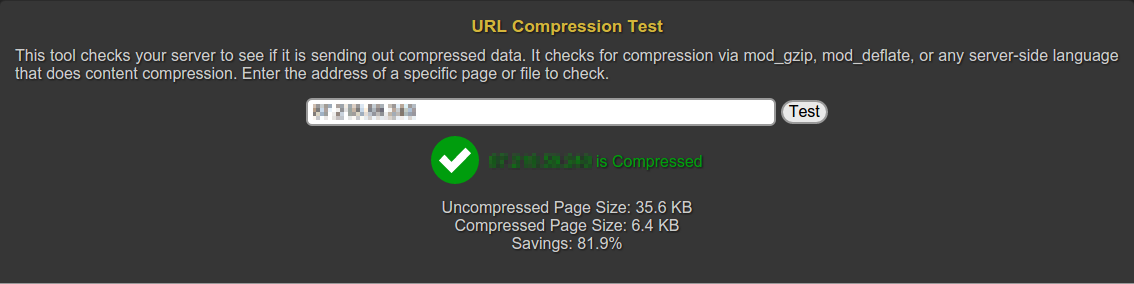
\includegraphics[width=\linewidth]{express_compression}
  \end{center}
  \caption{Express Middleware: Compression. Results of compression test (81.9\%)\\(Source: \url{http://www.whatsmyip.org/})}
  \end{figure}
  \item \textbf{Busboy}: HTTP Request parsing middleware. Parses the HTTP request and allows events to arise on certain types of
  requests like POST requests with files attached. This is used in HRUI to upload a map from the client to the server and save it on the
  server.
  \begin{figure}[H]
  \centering
  \captionsetup{justification=centering}
  \RecustomVerbatimEnvironment{Verbatim}{BVerbatim}{}
  \begin{minted}[fontsize=\footnotesize]{javascript}
  //Setup map upload http response
  var busboy = require('connect-busboy');
  app.use(busboy());
  //a POST request is made to /mapupload with a file attached to it.
  app.post('/mapupload', function(req, res) {
      var fstream;
      req.pipe(req.busboy);
      //event handler when busboy detects a file attachment.
      req.busboy.on('file', function(fieldname, file, filename) {
          //write attached file to disk asynchronously.
          console.log("HRUI: Uploading " + filename + ' to public/images/uploadmap');
          fstream = fs.createWriteStream(__dirname + '/../public/images/uploadmap');
          file.pipe(fstream);
          //once written to disk, respond to client.
          fstream.on('close', function() {
              res.send('Uploaded');
              console.log("HRUI: Uploaded " + filename + ' succesfully');
          });
      });
  });
  \end{minted}
  \caption{Express Middleware: Map Upload with Busboy code (Modified for clarity)}
  \end{figure}
  \item \textbf{Morgan}: Logger middleware. Logs to the console all HTTP requests along with the status and timing of the response.
  \begin{figure}[H]
  \captionsetup{justification=centering}
  \begin{center}
    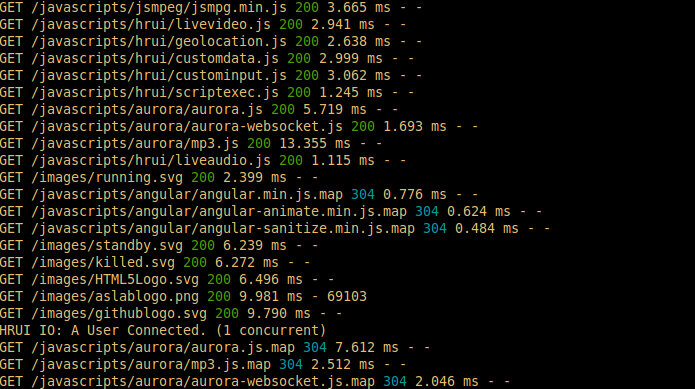
\includegraphics[width=0.7\linewidth]{express_logger}
  \end{center}
  \caption{Express Middleware: HRUI Example Morgan Logger Output\\(Normally configured to only show errors with response code > 400)}
  \end{figure}
  \item \textbf{Express Static}: This first-party middleware makes serving files from a directory as simple as: \mintinline{javascript}{app.use(express.static('public'));} Where 'public' is the folder containing the static content. This is useful in sites with few web
  pages, such as single-page applications like HRUI.
  \item \textbf{Serve Favicon}: Middleware to serve a favicon to web browsers. A Favicon is the icon that appears in modern browsers
  next to the URL in the search bar and in Bookmark bars. HRUI's Favicon is an NES Controller.\includesvg[height=12pt]{./img/favicon}
  \item \textbf{Custom Error Handling Middleware}: Instead of using some third-party error catching middleware, that would frankly be
  overkill, given that HRUI is a single-page application and is not designed for mass usage, making request errors infrequent, a small
  error handling middleware function was designed. It is placed at the end of all other middleware calls, meaning that if it's ever
  reached, no other middleware function could handle it. It generates a bit of HTML that presents the error to the user.
  \begin{figure}[H]
  \centering
  \captionsetup{justification=centering}
  \RecustomVerbatimEnvironment{Verbatim}{BVerbatim}{}
  \begin{minted}[fontsize=\footnotesize]{javascript}
  //Setup 404 error handler (if no handler before this is called, url not found)
  app.use(function(req, res, next) {
      var err = new Error('Not Found');
      err.status = 404;
      next(err);
  });
  // Display error in html.
  app.use(function(err, req, res, next) {
      res.status(err.status || 500);
      res.send('<h1>Error: ' + err.status + '<br>' + err.message + '</h1>' +
          '<h3>Description: ' + req.url + ' was not found.</h3>');
  });
  \end{minted}
  \caption{Express Middleware: HRUI Error handling custom middleware}
  \end{figure}
  \begin{figure}[H]
  \captionsetup{justification=centering}
  \begin{center}
    \includegraphics[width=0.5\linewidth]{express_error}
  \end{center}
  \caption{Express Middleware: HRUI Error handling response}
  \end{figure}
\end{itemize}
Many other middleware modules are available for express, (Layout engines like Jade, that allow creation of templates to make dozens of
similar pages without having to write each one independently. Cookie parsers. etc.) and many more are being developed, making it a very
versatile, lightweight alternative to traditional servers like Apache or Nginx.
\subsection{MongoDB} \label{mongodb}
\begin{figure}[H]
  \captionsetup{justification=centering}
  \begin{center}
    \includegraphics[width=0.7\linewidth]{mongodb}
  \end{center}
  \caption{MongoDB Logo}
\end{figure}
MongoDB (the name is derived from huMONGOus) is a NoSQL (Not Only SQL (Structured Query Language)) database. A NoSQL database does not
use a relational model, or as the acronym suggests, can use other models as well. The relational model (developed by Edgar Frank Codd in
1970) basically uses a table to store data with logic bindings on each row, called relations.
\begin{figure}[H]
  \captionsetup{justification=centering}
  \begin{center}
    \includegraphics[width=0.6\linewidth]{mongodb_relational}
  \end{center}
  \caption{MongoDB: Relational Database Example.\\(Source: \url{http://www.careerbless.com/})}
\end{figure}
This model was so extended before NoSQL databases that a special-purpose semi-standard programming language was developed for these DBMS
(DataBase Management System). The relational model, while still very much prevalent in web development, has problems with horizontal
scalability (using networks of computers to host large databases, required specially for big data applications), performance (querying
speed is largely affected by the size of the database and the complexity of the query) and it can be overly complex in design. NoSQL
databases on the other hand tend to be much faster and scalable, with simpler models, but sacrifice some consistency when compared to
relational databases. This makes NoSQL adequate for applications that require large amounts of distributed data and applications that
require very fast read/write operations. HRUI in its current state, only requires the latter, as the database is the interface with
which controllers access and write data to and from the model (see section \ref{mvcpattern} on the Model-View-Controller pattern),
making the speed of database I/O crucial. In section \ref{scalability} of chapter \ref{futuredevelopment} the possibility of scaling
HRUI horizontally in future development is discussed.\\

MongoDB is a document-based database. This model is very simple, in that the database is merely a collection of objects (documents),
each containing data regarding each object. Each document can have any amount of attributes that can be completely unrelated to the
attributes of other documents. A MongoDB database is best described as a collection of objects or ``things'' without any obligation to
be related to one another. This makes it very simple to implement, as almost no restrictions apply to documents, in contrast with the
rigid nature of tables in the relational model.\\

MongoDB uses JSON (JavaScript Object Notation) to describe documents. Again, striving for simplicity, JSON can be defined very
succinctly (see \url{http://json.org/}), and is of course very well suited to use with Node.js, given that no translation is required
when reading and writing to the database. It should be noted that documents aren't stored in this format in MongoDB, using instead BSON
(Binary JSON), which transforms JSON into binary data for enhanced performance.
\begin{figure}[H]
\centering
\captionsetup{justification=centering}
\RecustomVerbatimEnvironment{Verbatim}{BVerbatim}{}
\begin{minted}{javascript}
{
    "_id": 0,
    "item": "joystick",
    "x": "0.00",
    "y": "0.00",
    "mode": "lock4ways"
}
{
    "_id": 2,
    "item": "robotGeolocation",
    "latitude": 40.496534,
    "longitude": -3.877457,
    "accuracyRadiusInMeters": "5"
}
{
    "_id": 4,
    "item": "profiles",
}
\end{minted}
\caption{MongoDB: HRUI Initial JSON Documents (abridged for brevity)}
\end{figure}
The fact that MongoDB uses JSON as a format, doesn't imply that it's only suitable for use with programs written in JavaScript. With SQL
not being a suitable language, MongoDB uses drivers to be accessed from programs, apart from the "mongo shell" interactive command line
tool. These drivers are essentially libraries that supply simple calls to query, insert, delete documents and so on from the database.
Drivers are available for all modern programming languages (C/C++, C\#, Java, Python...\cite{mongodb11}) and allow for simple, fast
communication with the database.
\begin{figure}[H]
\centering
\captionsetup{justification=centering}
\RecustomVerbatimEnvironment{Verbatim}{BVerbatim}{}
\begin{minted}{python}
#Import mongoDB driver
import pymongo
from pymongo import MongoClient
#Connect to MongoDB local instance
mongoclient = MongoClient()
db = mongoclient.hrui
data = db.data
#Obtain a Python dictionary representing the document
deviceData = data.find_one({"item": "deviceData"})
#use data
thrust = float(deviceData['devOrientation']['beta'])
\end{minted}
\caption{MongoDB: CrazyFlie Python Controller MongoDB usage (abridged for clarity)}
\end{figure}
This is specially useful for HRUI, as back-end controllers that read/write data from the model can be written in the developers choice
of language, making it extremely simple to integrate controllers for any robot, in any language. This decoupling of the user interface
with the actual robot controller will be discussed further in section \ref{mvcpattern} on the MVC pattern. On the other hand, although
the drivers are generally simple to use and implement, it would be better to have a universal solution like SQL, which is still the
biggest issue with NoSQL databases as opposed to SQL databases: lack of standardization and documentation. Still, it's very simple to
use a Python or Node.js script that extracts data from the database and relays it to whatever other program using RPC (Remote Procedure
Calls) software or middleware such as CORBA (Common Object Request Broker Architecture), or raw sockets. This circumvents using the more
cumbersome MongoDB drivers, while sacrificing some performance by using an interpreted language (generally negligible for most
applications). The latter is used in the Khepera III controller for control over a TCP/IP network and is briefly explained in section
\ref{kheperaIII}.
\newpage
\subsection{AngularJS} \label{AngularJS}
\begin{figure}[H]
\centering
\includesvg[width=0.7\linewidth]{./img/angularjs}
\caption{AngularJS Logo}
\end{figure}
AngularJS is a front-end web application framework that uses an MVC (Model-View-Controller) architecture for the design of client-side
applications. The MVC architecture implemented by AngularJS allows for very clear separation between declarative code and business
logic, keeping client-side applications well structured and modular. It's important to point out that the MVC pattern used by AngularJS
applies only to the front-end of the application, not the overarching architecture of the application as a whole, which is itself an MVC
paradigm.\\

In the AngularJS framework, declarative code stays separate from business logic. The declarative code (HTML) is the \textbf{View} in the
architecture, while business logic is implemented by \textbf{Controllers} (JavaScript). The controllers act upon the \textbf{Model},
which are a collection of JavaScript objects that are bound to the controllers scope (the parts of the model the controller has access
to). AngularJS then modifies the view dynamically when the model is changed. It's important to emphasize the difference between this
architecture and modifying the DOM (Document Object Model, see section \ref{HTML} for more) directly from JavaScript. When doing the
latter, there is no model, and thus no way of knowing what piece of code changed the DOM and why, leading to confusing, difficult to
maintain and inelegant code. With "the Angular way", the controller that has access to a certain part of the DOM is declared in HTML,
and more importantly, the variables that are bound in the DOM to the model are also explicitly declared in the HTML. By looking at the
HTML, one can instantly know which elements correspond to model variables, because they are declared as such. To do this, Angular has
custom attributes added to HTML tags. These attributes are called directives, and declare the behavior attached to the element in
question. For example the ``ngModel'' directive, attaches the value of an element to the value of a variable in the scope of a
controller. If this is attached to a checkbox, for example, when a user (considered a controller in the architecture) changes the state
of the checkbox by clicking it, the model will be updated and the variable in the scope of the controller will change to false or true
accordingly. The controller will then be able to use that model variable to implement the business logic that the change of state in the
checkbox requires. This is exactly what is done in HRUI, when checking modules on and off ("data-" prefix added to ng-model for HTML
Validation, as custom attributes require data- or x- prepended):
\begin{figure}[H]
  \captionsetup{justification=centering}
  \begin{center}
    \includegraphics[width=0.5\linewidth]{angular_joystick}
  \end{center}
\end{figure}
\begin{figure}[H]
\centering
\captionsetup{justification=centering}
\RecustomVerbatimEnvironment{Verbatim}{BVerbatim}{}
\begin{minted}[fontsize=\footnotesize]{html}
<html data-ng-app="HRUI" data-ng-controller="HRUIController">
<!--...-->
<input id="joystickCheckbox" type="checkbox" data-ng-model="joystickOn"
data-ng-click="updateControls(event, joystickOn)">
<!--...-->
\end{minted}
\end{figure}
\begin{figure}[H]
\centering
\captionsetup{justification=centering}
\RecustomVerbatimEnvironment{Verbatim}{BVerbatim}{}
\begin{minted}[fontsize=\footnotesize]{javascript}
//...
app.controller('HRUIController', ['$rootScope', '$scope', 'SocketSrv', 'ProfileSrv',
    function(rootScope, scope, SocketSrv, ProfileSrv) {
        scope.joystickOn = false;
    //...
    //extract updated control from event, and notify back-end of selected controls
    scope.updateControls = function(control, newValue) {
        var changedControl = control.target.attributes.id.value;
        scope.sendControl(changedControl, newValue);
    };
\end{minted}
\caption{AngularJS: HRUI Checkbox Example (abridged for clarity)}
\end{figure}
In the HTML, the controller is declared (in this case for the entire document, as it's the master controller), and the directives are
assigned. The state of the checkbox (false equals unchecked) is bound to the scope variable joystickOn, which is initially false,
through the ngModel directive. The ngClick directive declares that the function called when the checkbox is clicked is updateControls,
that in this case sends the new state of the checkbox back to the server so it can process the actions that are necessary (sendControl,
not shown, uses Socket.IO to send the new value of the checkbox to the server via WebSockets. See section \ref{html5websockets} for
more).\\

This is just a small example of what can be achieved with what the creators of Angular call two-way data-binding. What this means is
that what is represented in the browser is simultaneously a variable in JavaScript, and can be modified by the user or controllers
indistinctly. The possibilities with this architecture are endless. Many of these directives are used in HRUI to create a dynamic 
single-page application very similar to what is expected of native desktop apps in terms of performance and responsiveness.\\

The concept of controllers that act upon different subsections of the DOM also allows for self contained modules to be added and removed
at will from an application, without the need to rewrite the whole JavaScript code. Since each controller is an independent entity, that
controls a part of the application without interference from other controllers, complex applications such as HRUI become very easy to
develop. The main benefits of this modularity are evident: once a module has been added and works correctly, more modules can be added
without any fear of breaking previous functionality, as there is no overlap in code; not all modules need to be active at any given
time, since each is independent, the user can select the relevant modules for each use-case on the fly; from a programmers perspective,
the code is very well compartmentalized making it easy to understand, maintain and improve upon; also from a programmers perspective,
code reuse is made simple, writing a controller once, using it in several parts of the application, or in other applications (following
the mantra DRY ``don't repeat yourself'. This is used in HRUI, with the same controller code attached to both joysticks, creating two
instances of the same controller); from a performance perspective, since modules are active only when they are used, there is no excess
resource usage.\\

Describing each of the directives used in detail would take up too much space, and would be hardly relevant to the subject at hand. Only
a couple of the more interesting directives used will be discussed briefly.
\begin{itemize}
  \item \textbf{ngIf}: The ngIf directive, allows elements to be added or removed from the DOM when the expression it evaluates is true
  or false respectively. This is a very important part of HRUI, that on startup seems empty, until the user starts turning modules on 
  (or loading a previously save profile, as explained in \ref{profilemanagement}) and these seem to appear in the browser. This is what
  allows the user to tailor the interface in a way that suits the use-case, and allows for performance to scale with the number of
  active modules.
  \item \textbf{ngAnimate}: This directive allows modules entering and exiting the application to have a visual effect when doing so.
  This uses a combination of CSS3 Transitions (see sections \ref{CSS} and \ref{html5styling}) and Pseudo-classes created by Angular to
  make modules fade-in and fade-out.
  \item \textbf{Custom Directive Touch}: The same way Angular lets the programmer create controllers, it allows the creation of custom
  directives. In HRUI, there is one custom directive used to add touch functionality to canvas elements (see section
  \ref{html5canvaselement}). This directive is bound to both the joystick canvases as wellas the map canvas, and uses handler functions
  to bind touch events to the equivalent mouse events. This is necessary only in canvas elements, as the rest of touch interactions are
  handled on the browser level.
  \begin{figure}[H]
  \centering
  \captionsetup{justification=centering}
  \RecustomVerbatimEnvironment{Verbatim}{BVerbatim}{}
  \begin{minted}[fontsize=\footnotesize]{javascript}
  app.directive('touch', function() {
      return {
          link: function(scope, element, attrs) {
              element.on('touchmove', function(event) {
                  scope.touchMove(event);
                  scope.$apply();
              });
              element.on('touchdown mousedown', function(event) {
                  scope.mouseDown(event);
                  scope.$apply();
              });
              element.on('mousemove', function(event) {
                  scope.mouseMove(event);
                  scope.$apply();
              });
              element.on('mouseup touchend', function(event) {
                  scope.mouseUp(event);
                  scope.$apply();
              });
          }
      }
  });
  \end{minted}
  \end{figure}
  \begin{figure}[H]
  \centering
  \captionsetup{justification=centering}
  \RecustomVerbatimEnvironment{Verbatim}{BVerbatim}{}
  \begin{minted}[fontsize=\footnotesize]{html}
  <canvas id="joystick" class="canvas joystick" data-touch>
  <canvas id="joystick2" class="canvas joystick" data-touch>
  <canvas id="mapcanvas" class="canvas" data-ng-show="mapOn" data-touch>
  \end{minted}
  \caption{AngularJS: HRUI Touch Directive (HTML abridged for clarity)}
  \end{figure}
  \item \textbf{Custom Directive Compile}: This directive allows the generation of HTML dynamically. This is required in the Custom 
  Input module (see section \ref{custominput}) to generate the HTML controls that the user has required. With the form data entered by 
  the user detailing what kind of inputs are required, an HTML table is created (function generateInputTable) that then needs to be 
  compiled into the DOM with the data-bindings to the model required. It's somewhat complex, but it allows for custom inputs to be 
  generated on the fly, adding great versatility to the interface.
    \begin{figure}[H]
  \centering
  \captionsetup{justification=centering}
  \RecustomVerbatimEnvironment{Verbatim}{BVerbatim}{}
  \begin{minted}[fontsize=\footnotesize]{javascript}
  app.directive('compile', function($compile) {
    return function(scope, element, attrs) {
        scope.$watch(
            function(scope) {
                // watch the 'compile' expression for changes
                return scope.$eval(attrs.compile);
            },
            function(value) {
                // when the 'compile' expression changes
                // assign it into the current DOM
                element.html(value);

                // compile the new DOM and link it to the current
                // scope.
                $compile(element.contents())(scope);
            }
        );
    };
  });
  \end{minted}
  \end{figure}
  \begin{figure}[H]
  \centering
  \captionsetup{justification=centering}
  \RecustomVerbatimEnvironment{Verbatim}{BVerbatim}{}
  \begin{minted}[fontsize=\footnotesize]{html}
  <table id="customInputTable" class="table" data-compile="customInputTable" 
  data-ng-if="customInputFormSubmitted"></table>
  \end{minted}
  \caption{AngularJS: HRUI Compile Directive}
  \end{figure}
\end{itemize}
Apart from controllers and directives, Angular (among many other features that are outside the scope of this report) implements 
services, to allow for communication between controllers, without interfering with each others scope. Services are "singletons" (in 
object-oriented programming, classes that can only have one instance at runtime) that contained shared methods or shared data. 
Controllers can claim access to a service and modify or bind to its data as well as call its functions. Since there's only one instance 
of a service, sharing data between controllers is reduced to writing or binding a service attribute and reading it from another 
controller. It also allows for code reuse (DRY ``don't repeat yourself') with functions that are used in several controllers being coded 
only once. There are 4 services in HRUI:
\begin{itemize}
  \item \textbf{ProfileSrv}: Allows controllers to publish the state of their scopes to the master controller, that then creates a
  profile with these states that can then be saved in the back-end for future use. See section \ref{profilemanagement} for more.
  \item \textbf{SocketSrv}: Holds the Socket.IO Websocket connection that needs to be accessed from all controllers to receive and emit
  events to the back-end, as well as media streaming raw WebSockets. See section \ref{html5websockets} on WebSockets.
  \item \textbf{DrawSrv}: Contains functions used to draw in Canvas elements: drawCircle, drawLineFromCenter and writeInCanvas (used in
  previous iterations).
  \item \textbf{GeometrySrv}: Contains functions used to calculate coordinates in Canvas elements: isInsideCircle, forceIntoCircle,
  centerCoord, canvasCoord, forceDirectionLock.
\end{itemize}
  \begin{figure}[H]
  \centering
  \captionsetup{justification=centering}
  \RecustomVerbatimEnvironment{Verbatim}{BVerbatim}{}
  \begin{minted}[fontsize=\footnotesize]{javascript}
  //Service with typical drawing methods shared between controllers
  app.service('DrawSrv', function() {
      return {
          drawCircle: function(ctx, x, y, radius, fillColor) {
              ctx.beginPath();
              ctx.arc(x, y, radius, 0, 2 * Math.PI, false);
              if (!!fillColor) { //if fillColor arg given, fill in circle.
                  ctx.fillStyle = fillColor;
                  ctx.fill();
              };
              ctx.stroke();
          },
          drawLineFromCenter: function(ctx, x, y) {
              ctx.beginPath();
              ctx.moveTo(ctx.canvas.width / 2, ctx.canvas.height / 2);
              ctx.lineTo(x, y);
              ctx.stroke();
          },
          writeInCanvas: function(ctx, font, text, x, y) {
              ctx.font = font;
              ctx.fillText(text, x, y);
          },
      }
  });
  \end{minted}
  \caption{AngularJS: HRUI DrawSrv Service example}
  \end{figure}
A full recap of the features of AngularJS is far beyond the scope of this report, but suffice it to say it's one of the core
technologies of this project, as the previous brief examples have shown. Without AngularJS, the Single-page Application wouldn't be as
responsive and immediately easy to use; the front-end code would be much less readable and as a result much more difficult to maintain
and build upon. As it is, a new front-end module can be added to the application very fast, so much so that the modules added later in
the development (gamepad, device motion and voice commands) took just a few hours to develop on the front-end, in part because of the
excellent modularity provided by the AngularJS framework that had been implemented previously. AngularJS is supported by Google and has
extensive and exhaustive documentation online\cite{google10}, both of which make it a very reliable framework to use, although a bit
daunting at first.
\newpage
\section{Development Environment \& Tools}
This section briefly describes the software development environment, software tools used to develop the project as well as
the robots used to demonstrate the integration of the project with existing hardware and simulated robots. The development
environment comprises the operating system (OS) used for development and deployment of the project, the source code editor
and build management software as well as the revision control system.
\subsection{Linux} \label{linux}
\begin{figure}[H]
\centering
\subfloat{\includesvg[width=0.2\linewidth]{./img/tux}}
\subfloat{\frame{\includesvg[width=0.6\linewidth]{./img/mint}}}
\caption{Tux the penguin, Linux mascot and Linux Mint Official Logo}
\end{figure}
Linux is the OS of choice for software development. The Linux distribution used in this project is Linux Mint 17 (Qiana) - 17.1(Rebecca)
Cinnamon Edition (64-bit version), that is based on the Ubuntu distro, itself based on Debian. A description of the Linux kernel and the
distribution used in this project is far beyond the scope of this report, but the choice to develop and deploy the application on this
platform will be discussed briefly.\\

The main reason why this project was developed on Linux is because of how easy it makes the installation and use of development tools 
through package management systems. A package management system automatically installs software and all of its dependencies (external 
software a program relies on to function) without having to manually download or install anything. This makes installing the needed 
software to develop this project as simple as  executing the command: \mintinline{shell}{ sudo apt-get install nodejs npm mongodb python2
}, which will install any dependencies required and will configure the programs for use. In Microsoft Windows, no official package 
management is implemented (although third-party package managers exist, like "chocolatey"), so installation and configuration of node, 
npm, python and mongodb has to be performed manually, with the ensuing troubleshooting. This applies to most Linux distributions, making 
it very simple to translate the installation and development requirements from one distribution to another. The Raspberry Pi 2 (see 
section \ref{raspberrypi2}) used as a portable server in this project, uses an Arch Linux distribution, but the installation is roughly 
the same: \mintinline{shell}{ sudo pacman -Syu install nodejs npm mongodb python2}, using the Pacman package manager. This portability 
offered is just one of the many reasons (configurable, wealth of development tools, command-line interface, scripting, etc.) that Linux 
is the main software development platform of the world.

The application is designed to work best on a Linux server, like the majority of web servers publicly accessible on the Internet.
However, given that one of the objectives of the project is accessibility to both the front-end of the application and the back-end, the
server works on any machine capable of running Node.js (see section \ref{nodejs}) and MongoDB (see section \ref{mongodb}). The only
caveat to the use on systems other than Linux is the loss of media streaming capabilities, that rely on Linux dev files to access video
and audio hardware. The main reason Linux is used as a server platform is for its stability and reliability. Windows machines require
regular maintenance and reboots to work properly while Linux is generally much more stable.
\subsection{Sublime Text}
\begin{figure}[H]
\centering
\includegraphics[width=0.2\linewidth]{sublime}
\caption{Sublime Text Logo}
\end{figure}
Sublime Text is the text and source code editor used in this project. It's not a traditional IDE (Integrated Development
Environment) like Eclipse or NetBeans, but includes many of the features found in those, implemented through user developed
plug-ins that are installed through a package management system of it's own: Package Control. Some of these features are:
\begin{itemize}
  \item Project file management: Create custom project file trees to access on the fly from the sidebar.
  \item Multiple editor tabs and file map: Edit code side by side, very useful when developing front-end and back-end of a module in
  HRUI, and visual map of file on the right side of the screen for quick scrolling, useful for tracking sections in code or in \LaTeX
  source.
  \item Customizable build systems: Create scripts that run custom commands to build or execute the source.
  \item Language-specific code highlighting and coloring: Helps visual orientation in code.
  \item Automatic code formatting: Runs a script that automatically refactors the code for readability, with correct indentation and
  trailing spaces.
  \item Code completion and code snippets: Auto-completes variable, function and typical programming structures (functions, objects, 
  if-else if) for convenience.
  \item Refactoring tools: Make changes to code that affect several parts of the project instantly, e.g. changing a variable name across
  the whole application once, instead of in each instance of the name.
  \item Version control integration: Run version control (see section \ref{git}) commands directly from the editor.
  \item Scripting tools: Such as a CSS auto vendor prefixer (adds vendor specific prefixes to CSS code automatically when including a
  conflicting CSS rule) or javascript/CSS minifier (reduces the size of javascript/CSS files by refactoring text, saving network
  resources).
  \item Aesthetic customization: Modify the UI for visual comfort.
\end{itemize}
Sublime Text was used for both the development of the source code as well as for this report in \LaTeX.
\begin{figure}[H]
\centering
\subfloat{\includegraphics[width=0.5\linewidth]{sublime_hrui}}
\subfloat{\includegraphics[width=0.5\linewidth]{sublime_report}}
\caption{Sublime Text: HRUI and Report Development Environment}
\end{figure}
\subsection{PM2}
\begin{figure}[H]
\centering
\includegraphics[width=0.6\linewidth]{pm2}
\caption{PM2 Logo}
\end{figure}
PM2 is a process manager that supplies Apache-like server management. Node.js (see section \ref{nodejs}) creates the possibility of
lightweight asynchronous web servers through frameworks like Express (see section \ref{express}). This is very useful, but Node is still
just a process on a server: if for whatever reason the application crashes or the server restarts, there is no service that restarts the
application or starts the web server on boot. That is where programs like PM2 come in, keeping the web server running, balancing its
load and restarting it if need be. It also has process monitoring and management options. PM2 is itself installable through the Node
Package Manager, NPM, as it is a Node.js module.\\

With PM2 the application can be set to start on boot, and restarted automatically if any crashes occur, with a 0 s reload downtime,
giving a reliable solution for long term use of the server. This is used in this project to implement the portable server using the
Raspberry Pi 2 (see section \ref{raspberrypi2}). PM2 is configured in the embedded Linux OS to start the app on boot and keep it alive,
allowing the board to act as an ``out of the box'' server for use anywhere with no configuration, except connection to a given network
via Ethernet or Wifi.\\

PM2 was also used throughout the development of the application, taking advantage of its file monitoring capabilities. PM2 can be
configured to restart the application if any of the files in its directory are modified. This was extremely useful in creating an agile
workflow for development. The PM2 service was started with this option enabled and the server would start. Modifications and additions
were made to the source code and upon save, PM2 would detect the change and restart the application wit the new source automatically.\\

Other PM2 features used throughout development were its memory and CPU monitoring and logging tools. Logging showed the console output
of the app for debugging and the monitoring feature helped detect memory leaks and inefficiencies in testing.
\begin{figure}[H]
\centering
\includegraphics[width=0.6\linewidth]{pm2example}
\caption{PM2: PM2 list, monit and logs command output example}
\end{figure}
\subsection{Git \& GitHub} \label{git}
\begin{figure}[H]
\centering
\subfloat{\includegraphics[width=0.3\linewidth]{git}}
\subfloat{\includegraphics[width=0.4\linewidth]{github}}
\caption{Git and Github Logo}
\end{figure}
Git is a distributed revision control system developed by Linus Torvalds, the creator of the Linux Kernel. A revision control system is
used in software development to track changes to the source code of a project. The distributed nature of Git allows multiple developers
to work on a project merging the changes made by all of them to a single or multiple versions of the code, keeping track of all changes,
so that they can be automatically reversed or superseded if necessary. This aspect of Git wasn't used in this project, as there was only
one developer, but revision control is also useful in this use-case. With Git, a code repository is created, wherein all of the code is
placed. The code in the repository is tracked for changes, and when the developer deems it appropriate (normally when a large change or
several smaller changes are made to the code), the changes are "committed" to Git. This ``commit'' is then "pushed" to the repository,
establishing a new version of the code, with a short message attached to it, explaining the changes. The cycle then restarts. For multi-
developer projects, another step is required: ``pulling'' the latest version from the repository  before making changes. If this is not
done, the changes can be ``merged'' if the changes do not conflict with the latest commit.\\

GitHub is a web service that hosts public Git repositories free of charge. It also maintains statistics on the development and the code,
 some of which are used in section \ref{planning} on Project Planning. GitHub was used in this project to host both the 
\href{https://github.com/xpeiro/HTML5RUI}{project repository} as well as \href{https://github.com/xpeiro/PFC}{this report's repository}, 
as well as for the use of public repositories for the JavaScript MPEG1 decoder \href{https://github.com/phoboslab/jsmpeg}{JSMpeg}, the 
Voice recognition library \href{https://github.com/TalAter/annyang}{Annyang} and the MP3 JavaScript decoder 
\href{https://github.com/audiocogs/aurora.js/}{Aurora.js} and their respective documentation. GitHub also allows the possibility of
hosting static web pages. This features is used to include a version of the User Manual (see section \ref{usermanual}) online at: 
\url{http://xpeiro.github.io/hrui/index.html}.\\

Revision control in general has many benefits:
\begin{itemize}
  \item Revert changes that result in issues: Since all previous versions are stored, the code can be reverted to any previous version
  very simply.
  \item Detect source of issues: When a bug or issue with the application arises that was not previously present, revision control can
  make it very easy to pinpoint which commit created the problem, by testing previous versions and testing which one first had the bug,
  making debugging easier.
  \item Backup: By using a hosting service like GitHub the code is protected from local hardware/software failures and errors. In
  distributed revision control, several copies of the code exist at any given time on different servers.
  \item Code history or statistics: analysis of work load and work performance is easier with data on who changed the code, when, why
  and how many times.
  \item Compartmentalization: Experimental changes to code can be made without affecting a working version of the code, eliminating
  chances of breaking code inadvertently.
  \item Sharing: services like GitHub make sharing code very simple.
\end{itemize}
\subsection{\LaTeX}
\LaTeX\ (pronounced ``Lah-tech'') is an open source procedural markup language for document preparation originally developed by Leslie
Lamport based on the \TeX typesetting system by Donald Knuth. It's widely used to create scientific and technical documentation, such as
this report. It's comprised of a series of macros (text that is processed to be replaced with other text) for the underlying \TeX\
typesetting system. It has several advantages over the more common WYSIWYG (``What You See Is What You Get'') word processors like
Microsoft Word (the de facto alternative):
\begin{itemize}
  \item Separation between content and presentation: The content is not tied to the presentation, rather the presentation can be changed
  using macros without modifying the content, which is simple text.
  \item Referencing: Powerful tools are available to make cross references in large documents like the ones made in this document when
  referring to sections.
  \item Automatic Numbering and Indexing: The cross references made do not make reference to the numbers of the sections. This numbering
  is generated by \LaTeX\ automatically and references are macros that fill in with the correct number on compilation. This is also used
  for the bibliography.
  \item Automatic Table of Contents and Figures: The table of contents is auto generated with the sections on compilation. Likewise the
  table of figures is generated with the existing figures (also numbered automatically).
  \item Better content embedding: Inserting images and graphics is much simpler and organized.
  \item Development Community: Creates hundreds of packages that are useful for all kinds of different use-cases whereas commercial
  solutions require limited features for broad appeal.
  \item Compatibility: \LaTeX\ source from 20 years ago can still produce a document today. Word documents cannot, without significant
  modifications.
  \item Revision Control: \LaTeX\ source can be easily put under version control, whereas this feature in Microsoft Word is very limited.
  \item Source readability: Word .docx files are essentially zipped XML, which is very hard to read. \LaTeX\ commands on the other hand
  are very close to their meaning and do not interfere with the content as much.
  \item Source Commenting: Adding comments to the source, more information can be added on how the document should be presented and why.
  \item Open Source: Can be modified at will with added packages that provide new functionalities.
\end{itemize}
  \begin{figure}[H]
  
  \captionsetup{justification=centering}
  \RecustomVerbatimEnvironment{Verbatim}{BVerbatim}{}
  \begin{minted}[fontsize=\footnotesize]{latex}
%   HTML5 Robot User Interface Project Report
%   An ASLab Project,
%   Developed by Daniel Peiró
%   ETSII, UPM 2014-2015

% Define Document Type, Font size, Paper size, and input/output encoding.
\documentclass[12pt,twoside,a4paper]{report}
\usepackage[T1]{fontenc} 
\usepackage[utf8]{inputenc}

%%%%%%% Formatting Section %%%%%%%%

% Document formatted according to PR/CL/1/001,
% Annex ANX-PR/CL/1/001-01, available at:
% http://www.industriales.upm.es/la_escuela/doc/Procedimiento-TFG-TFM-PFC-def.pdf
%
% Font: Times New Roman, 12 points.
% Margins: All 1 in.
% Header and footer content: Defined in 'plain' page style. 

\usepackage{mathptmx} % Times New Roman.
\usepackage[top=1in, bottom=1in, left=1in, right=1in]{geometry} % 1 in. Margins.
\usepackage{fancyhdr} % Header/Footer formatting.
  \end{minted}
  \end{figure}
  \begin{figure}[H]
  
  \captionsetup{justification=centering}
  \RecustomVerbatimEnvironment{Verbatim}{BVerbatim}{}
  \begin{minted}[fontsize=\footnotesize]{latex}
\pagestyle{plain} %Set Document Page Style to plain
\setlength{\headheight}{15pt} % Header height 15 points.
\setcounter{tocdepth}{4} % Set Table of Contents sectioning depth
\setcounter{secnumdepth}{4} % Set Table of Contents numbering depth
\fancypagestyle{plain}{
    \fancyhf{} %Clear Defaults.
    \renewcommand{\headrulewidth}{1pt} % Header horizontal rule.
    \renewcommand{\footrulewidth}{1pt} % Footer horizontal rule.
    \fancyhead[LE]{\nouppercase\leftmark} % Even Pages: Chapter and Section Name, top left.
    \fancyfoot[LE]{\thepage} % Even Pages: Page number, bottom left.
    \fancyfoot[RE]{Escuela Técnica Superior de Ingenieros Industriales (UPM)} 
    % Even Pages: University name, bottom right.
    \fancyhead[RO]{HTML5 Robot User Interface} % Odd pages: Project name, top right.
    \fancyfoot[RO]{\thepage} % Odd pages: Page number, bottom right.
    \fancyfoot[LO]{Daniel Peiró Moreno}  % Odd pages: Author, bottom left.
}
%%%%% End Formatting Section %%%%%%

% Title, Author and Date
\title{HTML5 Robot User Interface}
\author{Daniel Peiró Moreno}
\date{2015}

%%%%%% Import Packages %%%%%%
\usepackage{graphicx}
\usepackage{svg}
\usepackage{subfig}
\usepackage{epigraph}
\usepackage{hyperref}
\usepackage{makeidx}
\usepackage{minted}
\usepackage{lipsum}
%%%% End Import Packages %%%%

\begin{document}

% 	HTML5 Robot User Interface Project Report: Acknowledgements
% 	An ASLab Project,
% 	Developed by Daniel Peiró
% 	ETSII, UPM 2014-2015

\chapter*{}
\vspace{120pt}
\epigraph{\textit{Para Cristina, por hacerlo posible.}}{}
\vspace{90pt}
\epigraph{\textit{Ex Nihilo Nihil Fit.\\
Out of nothing, nothing becomes.}}{\textit{Titus Lucretius Carus\\De Rerum Natura}}

\tableofcontents
% 	HTML5 Robot User Interface Project Report: Summary
% 	An ASLab Project,
% 	Developed by Daniel Peiró
% 	ETSII, UPM 2014-2015
\chapter*{Resumen Ejecutivo\\(Executive Summary in Spanish)}

El objetivo de este proyecto es el desarrollo de \textit{software} que proporcione una interfaz gŕafica de usuario (en adelante 
\textit{GUI}) con una variedad de herramientas diseñadas para recoger entradas (\textit{inputs}) para el control de robots, asi 
como la presentación de las salidas (\textit{outputs}) de los mismos. Se desea que la aplicación (el programa) cumpla con los 
siguientes requisitos:
\begin{itemize}
	\item \textbf{Universalidad}: La GUI debe ser fácilmente adaptable al uso de un amplio abanico de robots, con diferentes 
	capacidades y características.
	\item \textbf{Accesibilidad}: Este requisito se divide en dos partes:
	\begin{itemize}
		\item La GUI debe ser fácilmente utilizable desde un amplio abanico de dispositivos, incluyendo como mínimo, 
		ordenadores de sobremesa (\textit{desktop}) y portátiles (\textit{laptop}), dispositivos móviles como teléfonos 
		inteligentes (\textit{smartphones}) y tabletas (\textit{tablets}), todos ejecutando distintos sistemas operativos, con 
		respecto a los cuales la aplicación debería ser agnóstica (debería ejecutarse indistintamente en cualquier SO).		
		\item La aplicación que proporcione la GUI debe además exponer una API (\textit{Application Programming Interface} o 
		Interfaz de Programación de la Aplicación) que permita a desarrolladores externos usar las entradas y salidas de la GUI 
		para cualquier robot o aplicación, consiguiendo asi realizar el primer requisito. Esta interfaz debe ser tan simple 
		como sea posible, y debe cumplir con todos los demás requisitos, donde sea aplicable (por tanto debe ser portable, 
		distribuida, en tiempo real y de código abierto (\textit{open source})).
	\end{itemize}
	\item \textbf{Personalizable (\textit{Customizable})}: Parcialmente debido al primer requisito, la GUI debe tener una 
	variedad de entradas y salidas que deben ser utilizables de manera independiente, de tal forma que múltiples 
	configuraciones puedan prepararse y ser usadas para diferentes robots, asi como para diferentes aplicaciones del mismo 
	robot. A ser posible, el usuario debería poder crear entradas y salidas personalizadas cuando las herramientas propuestas 
	sean insuficientes para la aplicación particular. Este proceso debería ser sencillo y transparente para el usuario, a ser 
	posible.
	\item \textbf{Distribuida}: Parcialmente debido al requisito de accesibilidad, la aplicación debe ser distribuida en red, de 
	manera que la GUI no esté físicamente atada a una máquina en particular, o tenga que ser ejecutada de manera local para 
	aportar la funcionalidad requerida.
	\item \textbf{Tiempo Real}: Las entradas registradas por la GUI deben ser capaces de controlar al robot en tiempo real. 
	Asímismo, las salidas del robot deben ser presentadas al usuario en tiempo real. No se establecen tiempos límite 
	(\textit{deadlines}) severos, dado que la aplicación es distribuida y por tanto estos tiempos serían difíciles de estimar sin 
	una investigación exhaustiva y control sobre el entorno de ejecución de la aplicación, lo cual negaría el requisito de 
	accesibilidad. Sin embargo, el tiempo de respuesta del sistema deberá minimizarse dentro de las posibilidades del estado del 
	arte de las tecnologías empleadas.
	\item \textbf{Portabilidad}: La aplicación que proporcione la GUI debe ser ejecutable en un amplio abanico de sistemas, con 
	respecto a estas variables:
		\begin{itemize}
			\item Prestaciones \textit{Hardware}: La aplicación debe ser ejecutable en ordenadores portables de bajo coste y 
			bajas prestaciones con el fin de ser montable sobre robots móviles si así se requiere.
			\item Sistemas Operativos: La aplicación debe ser multi plataforma, es decir, debe ser ejecutable en una variedad de 
			sistemas operativos. Estos SOs deben incluir, como mínimo: una distribución de uso general de Linux, Microsoft 
			Windows y Apple OS X. Solo las últimas versiones de cada uno deben ser soportadas. Se requiere soporte como mínimo 
			las siguientes arquitecturas: 32/64-bit x86.\\
		\end{itemize}
	\item \textbf{Código Abierto (\textit{Open Source})}: Todo el \textit{software}, bibliotecas (\textit{libraries}) y 
	\textit{frameworks} empleados en el desarrollo y uso de la aplicación deben ser de código abierto. Esto, a grandes rasgos, 
	supone que el \textit{software} sea libre para el uso, estudio y modificación del mismo para cualquier propósito. Las 
	implicaciones del código abierto se estudian en la memoria del proyecto como valoración de los impactos y aspectos de 
	responsabilidad legal, ética y profesional del trabajo. Las herramientas usadas para el desarrollo (Entornos Integrados de 
	Desarrollo \textit{IDEs}, SOs, \textit{hardware} etc.) no tienen porque ser de código abierto, pero se preferirán 
	herramientas que lo sean en caso de ser alternativas viables.\\
\end{itemize}
En esencia, la aplicación debe establecer un nexo entre las dos entidades principales del control de robots:
\begin{itemize}
	\item \textbf{El Usuario}: Requiere una interfaz para introducir comandos que el robot debe seguir. Asímismo, requiere una 
	vista de las datos de salida del robot, si están disponibles.
	\item \textbf{El Robot}: Necesita recibir comandos en un protocolo particular que entiende, para poder funcionar. Además, 
	opcionalmente, puede exponer datos de salida para que el usuario los vea o sean registrados.
\end{itemize}
En el siguiente diagrama UML (\textit{Unified Modeling Language}) simplificado,se muestran los tres componentes: el usuario, la 
aplicación y el robot. El objetivo del proyecto es el desarrollo del componente central, la aplicación, junto con las interfaces 
que expone tanto al usuario como a robot, o con mayor precisión al controlador del robot, que traducirá la interfaz de la 
aplicación a la interfaz que entiende el robot.
\begin{figure}[H]
\centering
\captionsetup{justification=centering}
\includegraphics[width=\linewidth]{resumenuml}
\caption{Diagrama UML simplificado del objetivo del proyecto}
\end{figure}

Siguiendo un esquema de desarrollo en cascada iterativo (elaboración de requisitos, diseño, implementación y verificación, 
iterados para cada módulo de la aplicación, y finalmente mantenimiento), se planificó el proyecto. A continuación se procedió al 
estudio del estado del arte de las tecnologías que cumplen con estos requisitos y el diagrama de objetivos. Se diseñó una 
arquitectura del sistema que cumplía con los objetivos y se desarrolló la aplicación. Por último se probó el funcionamiento de la 
aplicación y se escribió la memoria del proyecto, en la que se describe en detalle el estado del arte de las tecnologías 
empleadas (capítulo 2), la arquitectura del sistema (capítulo 3), el desarrollo futuro (capítulo 4) y la planificación del 
proyecto (capítulo 5). Se incluye además como anexo el manual de usuario de la aplicación.\\

Los puntos básicos de la solución propuesta son los siguientes:
\begin{itemize}
	\item \textbf{GUI Modular en HTML5}: La GUI es una página web estrictamente en HTML5 (la última versión del estándar del 
	lenguaje empleado para diseñar páginas web). Esto propone una solución al requisito de accesibilidad, dado que las páginas 
	HTML5 son accesibles desde cualquier dispositivo capaz de abrir una página web. Esto incluye ordenadores, teléfonos 
	inteligentes y tabletas, así como una variedad de micro ordenadores. La modularidad proporciona una solución al requisito de 
	personalización, dado que cada módulo puede ejecutarse independientemente de otros, y por tanto cualquier permutación de 
	módules es posible.
	\item \textbf{Servidor Node.js}: La aplicación es un servidor web Node.js (una plataforma para ejecutar programas en el 
	lenguaje JavaScript como si fueran cualquier otro programa, en lugar de en el navegador. Está basado en el motor de 
	JavaScript de Google Chrome, es muy ligero y asíncrono). Dado que Node.js es multi plataforma, esto también aporta una 
	solución al requisito de portabilidad.
	\item \textbf{Arquitectura Cliente-Servidor}: Proporciona una solución al requisito  de ser una aplicación distribuida. El 
	clientes es la página web HTML5. El servidor es la aplicación que maneja las entradas y salidas del cliente. Pueden ser 
	ejecutados en máquinas distintas y se comunican vía Internet o en red local mediante varios protocolos.
	\item \textbf{Comunicación basada en \textit{WebSockets}}: Este protocolo de comunicación permite al cliente y servidor 
	comunicarse en tiempo real sobre una red de manera eficiente pasando mensajes entre ellos con paquetes de datos asociados, de 
	manera similar a los programas que se comunican entre sí mediante un \textit{socket} UNIX. Esto da respuesta al requisito de 
	tiempo real.
	\item \textbf{Arquitectura MVC (Modelo-Vista-Controlador)}: Propone una solución a los requerimientos de universalidad y 
	accesibilidad (segundo apartado), mediante el diseño de la aplicación. Se diseña de manera que la GUI (la Vista) está 
	desacoplada del estado de la aplicación (el Modelo), permitiendo así que desarrolladores externos accedan sencillamente al 
	Modelo, usando Controladores. Esto se llama doble-desacoplamiento (\textit{double-decoupling}) en el proyecto.
	\item \textbf{Entradas y salidas personalizables}: Como resultado de la prestación previa, el usuario puede crear nuevas 
	entradas y salidas dinámicamente, que son accesibles a la interfaz de la aplicación de manera instantánea y transparente. 
	Esto da respuesta al requisito de personalización.
	\item \textbf{Código abierto}: Todas las tecnologías empleados son de código abierto.
\end{itemize}
Los resultados del proyecto se detallan en el capítulo 6 de la memoria.\\

Como demostración del funcionamiento de la aplicación, se realizó la integración de la misma con tres robots distintos:
\begin{itemize}
	\item \textbf{Khepera III Virtual, en simulador V-REP}. Comunicado en Red.
	\item \textbf{Khepera III (Robot diferencial)}. Comunicado en Red inalámbrica.
	\item \textbf{Crazyflie 2.0. (Mini-Cuadrirotor)}. Comunicación por Radio.
	\item Parrot Rolling Spider (Mini-Cuadrirotor con estabilización de altura por ultra-sonidos). Comunicación por bluetooth. 
	(Nota: no documentado por ser muy parecido al anterior cuadrirotor).
\end{itemize}

Siendo las tres integraciones un éxito, ya que con controladores relativamente simples (el cuadrirotor requiere apenas 50 líneas 
de código para ser controlado totalmente en vuelo usando un mando con dos \textit{joysticks}) y en lenguajes de programación 
diferentes (la aplicación tiene interfaz con prácticamente cualquier lenguaje de programación moderno), se consiguió controlar y 
leer los datos en todos los casos en tiempo real, sin retrasos incluso usando redes móviles para la conexión vía internet.\\

Como demostración de la portabilidad de la aplicación, se integró en un micro ordenador de bajas prestaciones (4 núcleos a 900 
Mhz y 1 GB de RAM) y bajo coste (33 Euros), el Raspberry Pi 2. Esto permite, mediante una batería externa (5 V, 1.5 A), montar el 
micro ordenador (85x56x17 mm) en cualquier robot móvil, permitiendo su control vía internet desde cualquier dispositivo que pueda 
abrir un navegador, sin necesidad de ningún hardware intermedio (salvo, lógicamente la interfaz entre el micro ordenador y el 
robot, que comúnmente será en red TCP/IP, bluetooth, radio, serial, etc.).\\

La aplicación tiene las siguientes herramientas para uso con cualquier robot, otorgando una gran versatilidad:
\begin{itemize}
	\item \textbf{Módulos de entrada}: Utilizados para dar órdenes o de manera mas general, aportar datos a la aplicación y en 
	consecuencia al robot.
		\begin{itemize}
			\item Módulo de \textit{Joystick}: Joystick virtual, manipulable con el cursor o con el tacto (si el dispositivo es 
			táctil).
			\item Módulo \textit{Gamepad}: Permite conectar cualquier mando externo al dispositivo de control, y usarlo como 
			controlador del robot.
			\item Módulo de orientación del dispositivo: Permite usar los datos de orientación y movimiento del dispositivo como 
			controles para el robot (si el dispositivo tiene accelerómetros o equipos similares).
			\item Módulo de comandos por voz: Permite dar órdenes por voz al robot, mediante reconocimiento de lenguajes en línea 
			(requiere conexión a internet, disponible en varios idiomas, solo disponible en algunos navegadores).
			\item Módulo de entradas personalizadas: Permite al usuario crear entradas personalizadas (valores numéricos, 
			deslizadores, casillas booleanas o texto) dinámicamente y al instante, para suplir cualquier otro tipo de entrada no 
			contemplado.
		\end{itemize}
	\item \textbf{Módulos de salida}: Utilizados para presentar datos del modelo de la aplicación, normalmente datos del robot.
		\begin{itemize}
			\item Módulo de Monitorización de datos: Presenta la posición, orientación, velocidad y velocidad angular del robot, 
			además de un mapa de localización. El mapa puede ser generado dinámicamente, (útil para localización y mapeo 
			simultáneo, SLAM), puede ser estático en forma de imagen subida por el usuario o incluso pueden dibujarse obstáculos 
			dinámicamente con el cursor o tacto, para que sean reconocidos en tiempo real por el controlador del robot (mediante 
			una matriz binaria).
			\item Módulo de Vídeo en directo: Permite ver en directo una alimentación de vídeo proviniente de cualquier cámara 
			conectada al servidor. Útil para control remoto y FPV (vista en primera persona).
			\item Módulo de Audio en directo: Permite escuchar en directo (tiene un retraso de 2 segundos apróx.) una 
			alimentación de audio de cualquier fuente conectada al servidor.
			\item Módulo de Geolocalización: Presenta un mapa dinámico (usando Google Maps) de la geolocalización del robot, 
			siempre que se proporcionen los datos desde el robot a la aplicación.
			\item Módulo de salidas personalizadas: Permite al usuario visualizar cualquier dato de salida del robot que se 
			introduzca en la aplicación, que no haya sido contemplado por otro módulo.
		\end{itemize}
	\item \textbf{Módulos de Utilidad}: Disponibles para la comodidad del usuario.
		\begin{itemize}
			\item Módulo de ejecución de scripts: Permite al usuario ejecutar programas en el servidor de manera remota, siempre 
			que se hayan añadido a una localización concreta en el servidor (por seguridad).
			\item Módulo de administración de perfiles: Permite guardar y recuperar cualquier combinación de módulos con todos 
			sus datos, para poder configurar la interfaz de manera permanente para cada caso de uso. Útil particularmente para el 
			uso de gran cantidad de entradas personalizadas.
		\end{itemize}
\end{itemize}
El proyecto se realizó entre Agosto de 2014 y Agosto de 2015. Inicialmente debía entregarse en Marzo de 2015, pero debido a que 
el estudiante fue contratado como becario en Octubre de 2014, el trabajo del proyecto tuvo que relegarse al tiempo libre y fines 
de semana. La memoria está escrita en inglés porque al tratarse de un proyecto software, en el que la mayoría de los términos, 
lenguajes de programación, código escrito, comentarios de código, documentación de todos los sistemas empleados, fuentes de 
información etc. están en dicho idioma, se consideró más práctico el uso del mismo para documentar el proyecto.
% 	HTML5 Robot User Interface Project Report: Introduction
% 	An ASLab Project,
% 	Developed by Daniel Peiró
% 	ETSII, UPM 2014-2015

\chapter{Introduction}
\section{Lorem Ipsum}
% 	HTML5 Robot User Interface Project Report: Technology Overview
% 	An ASLab Project,
% 	Developed by Daniel Peiró
% 	ETSII, UPM 2014-2015
\chapter{Technology Overview} \label{technologyoverview}
This chapter will give a general overview of the technologies used in the development of this project. 
This will loosely entail, for each section, a brief history, the current state of the art and how it relates 
to the project. By no means is this intended to be a comprehensive in depth look into each subject, given that 
entire books can and have been written on each of them, but should give the reader enough information to understand 
the following chapter, that details how the system is built and what it does with these technologies.
\section{HTTP} \label{HTTP}
HTTP (Hypertext Transfer Protocol) is the data communication protocol underlying in what is known today as the World
Wide Web. The idea of hypertext (a text that contains links to other texts) was first defined in the 1960s by Ted
Nelson (inspired by the Memex, a microfilm linked database envisioned by Vannevar Bush in 1945), founder of Project
Xanadu, the first attempt at an implementation of the idea. Several other implementations appeared in the following
decades (Douglas Engelbart's oN-Line System, Apple's Hypercard, Tim Berners-Lee's own ENQUIRE), but none of them
married the concept with the idea of the Internet, which had been developed independently from it's origins (ARPANET
and TCP and later TCP/IP) in the late 1960s. Not until Tim Berners-Lee, a computer scientist working at CERN in 1989,
took his existing ENQUIRE hypertext database and the existing TCP/IP protocol and thought to make a network of
documents, linked between each other to form a web, that he called the ``WorldWideWeb'' or W3. To do that he needed
essentially three things: a standard language to write hypertext in, unique identifiers for each document and a
protocol to transfer these documents around the network. The first is HTML, which will be covered in the next section,
the second is the URL (Uniform Resource Locator, which won't be covered due to being only tangentially related to the
project) and the last of course is HTTP. There were other protocols that essentially achieved the same goal, most
notably Gopher, which still exists, but in the 1990s the World Wide Web became ubiquitous and synonymous with the
Internet, mainly thanks to the Mosaic Web Browser's popularity following its release in 1993. Today HTTP is the main
protocol (frequently combined with SSL/TLS to form the HTTPS protocol for enhanced security) used in the world to
communicate through the Internet.\\

HTTP implements a typical Client-Server stateless pattern with a request-response communication architecture. What
stateless means is that every transaction between client and server is independent from any other. In other words,
HTTP treats every connection as a new one, given that it has no ``memory'' of any others before it. The sequence of
events that define one transaction, define the whole protocol. The basic steps that take place in one such transaction
are:
\begin{enumerate}
\item The Client opens a connection to the server (through a TCP/IP socket, typically on the standard port 80) and
sends a request, which looks something like this:
\begin{minted}[breaklines,fontsize=\footnotesize]{http}
GET / HTTP/1.1
Host: www.w3.org
Connection: keep-alive
Accept: text/html,application/xhtml+xml,application/xml;q=0.9,image/webp,*/*;q=0.8
User-Agent: Mozilla/5.0 (X11; Linux x86_64) AppleWebKit/537.36 (KHTML, like Gecko) Chrome/43.0.2357.81 Safari/537.36
Accept-Encoding: gzip, deflate, sdch
Accept-Language: es-ES,es;q=0.8,en;q=0.6
Cookie: authorstyle=no
\end{minted}
This example is taken from a Chrome Browser ``development tools'' window (accesible with Ctrl+Shift+J), when opening
the \url{http://www.w3.org} URL.\\

This simple text message is asking the server to GET (HTTP Method) the path ``/'' (the root path) with version 1.1 of
the HTTP Protocol. The rest of the text is not required (HTTP 1.1 does require the Host Header to be present), but
adds additional information to the request. The Connection ``keep-alive'' header is added to use one TCP connection
for all requests and responses, instead of opening and closing a connection on each request, to reduce overhead (this
is standard in HTTP 1.1). The Accept Header tells the server what type of content it expects (in this case it prefers
html, xhtml or xml, or with less preference represented by the q value from 0 to 1, an image, or with even less
preference, anything else). The user agent tells the server which platform is making the request, and so on.
\item The server responds (through the same TCP connection):
\begin{minted}[breaklines,fontsize=\footnotesize]{http}
HTTP/1.1 200 OK
Date: Fri, 05 Jun 2015 17:13:20 GMT
Server: Apache/2
Content-Location: Home.html
Vary: negotiate,accept
TCN: choice
Last-Modified: Fri, 05 Jun 2015 14:20:15 GMT
ETag: "a290-517c5fda505c0;89-3f26bd17a2f00"
Accept-Ranges: bytes
Content-Length: 41616
Cache-Control: max-age=600
Expires: Fri, 05 Jun 2015 17:23:20 GMT
P3P: policyref="http://www.w3.org/2014/08/p3p.xml"
Content-Type: text/html; charset=utf-8
\end{minted}
Which indicates that using HTTP version 1.1, the request was attended correctly (code 200 OK), the server is an Apache
2.0 Server, the date and time of response, the name of the resource, the content type etc.
\item The connection is closed (in this case it would remain open since the protocol is version 1.1 and keep-alive was
specified).
\item The Server waits for another request on port 80.
\item The client uses the resource served. In most cases, the client would be a web browser, that would parse the
html, and present it to the user. This would in turn force the browser to request more resources (images, css,
scripts, etc.) that are embedded in the html (see figure \ref{http_requests}).
\end{enumerate}
\begin{figure}[h]
	\includegraphics[width=\linewidth]{http_requests}
	\caption{Google Developer Tools window showing HTTP Requests\label{http_requests}}	
\end{figure}

In the above example only the GET HTTP method is used, because the client only requests data from the server, without
sending any data itself. If the client needs to send data to the server, such as form data, or a file, it would still
initiate the connection (the server cannot make requests, only respond, another consequence of statelessness), using
the POST method. While this approach is suitable for a passive, document-based web, where interaction is limited to
jumping from document to document, the web has quickly evolved into an application-based model, where full UIs take
place in the browser space, requiring data be constantly sent back and forth between client and server, in realtime.
This project is one such application.\\

The only way to do this with standard HTTP is periodic polling, which entails large server and network loads. Some
stopgap solutions exist to minimize this overhead, most relevant of which is the Comet web application model. Comet is
based on the concept of long-polling: effectively ``hanging'' the server response until the requested data is
available, and calling another request once the data is received. This approach  still causes increased server loads
but allows some semblance of real-time data transmission. The possibility to use only one connection, as seen in the
previous example was another improvement that became standard in HTTP 1.1. With the HTTP/2 Standard (published in May
2015), the server is allowed to effectively ``push'' data to clients by queuing up more responses than received
requests. However, none of these modifications and hacks are a complete, elegant solution to the problem, given that
HTTP was never intended to be a real-time protocol.\\

That is why other technologies have taken over this new realm of interactivity, providing much more than the ``big,
virtual documentation system in the sky'' \cite{bernerslee09} envisioned by Berners-Lee more than 25 years ago. Some
of them are key parts of this project, as the following sections describe. Still, HTTP remains the initiator for all
these other technologies to function. As of today, any web page you open, no matter how complex the code served in
javascript or flash or any other plug-in still begins with a simple GET request and response.
\section{HTML} \label{HTML}
HTML (Hypertext Markup Language) is the language in which web pages are written. It was created in 1989 by Tim
Berners-Lee as part of his WorldWideWeb, a set of documents linked between each other on a network using the Internet
protocol. It was initially based on SGML (Standard Generalized Markup Language) a document markup language released in
1986 as an ISO Standard (ISO 8879:1986 -- Information processing -- Text and office systems), which was itself derived
from GML (both an acronym for Generalized Markup Language and for Goldfarb, Mosher, Lorie, the last names of its
developers), developed by IBM in 1969.\\

Markup languages in general existed before digital media and still exist in paper based documentation (blue/red
annotations used by editors because lithography/photography/xerography did not capture these colors, the engineering
code for editing documents red = add, blue = delete, green = comment, and many others). In general, markup is a way to
add information regarding the document's structure, presentation, state of development, comments, author, date,
copyright, etc. in a way that is distinguishable from the content of the document. For digital media, it also needs to
be machine-readable, which simply means that a computer must be able to parse this data to extract information. There
are basically two ways of doing this:
\begin{enumerate}
	\item Procedural Markup: A source text is written with instructions for a processing program (equivalent to a
  compiler) to construct the final document. A good example of this method is \TeX, the typesetting system underlying
  the \LaTeX\ macro language (which is itself a mixture of procedural and declarative markup), used to write this
  document.
	\begin{figure}[ht]
    \subfloat[Procedural Source (\LaTeX)]{{\includegraphics[width=\linewidth/2]{html_procedural_in}}}
    \subfloat[Procedural Output (PDF)]{{\includegraphics[width=\linewidth/2]{html_procedural_out}}}
    \caption{Procedural Markup Example}
	\end{figure}
	\item Declarative or Descriptive Markup: The content of the text is labeled or ``tagged'' with the markup, without
  giving any instructions on how to process these labels. HTML (especially before HTML5) and XML are clear examples of
  this method.
	\begin{figure}[ht]
    \subfloat[Declarative Input (HTML5)]{{\includegraphics[width=\linewidth/2]{html_declarative_in}}}
    \subfloat[Declarative Output (Google Chrome)]{{\includegraphics[width=\linewidth/2]{html_declarative_out}}}
    \caption{Declarative Markup Example}
	\end{figure}
\end{enumerate}
HTML and its precursor SGML are essentially declarative markup languages. The main advantage of declarative markup,
and more generally the declarative programming paradigm is the decoupling of the intended result and the processing
required to achieve it. This has been crucial for HTML to be able to evolve and adapt dynamically over decades of
technological innovation. The computers and programs used in 1989 have very little in common with those used today in
many cases. A markup language designed to be ubiquitous, read on an ever changing array of software and hardware
platforms and permanently backwards compatible, where a web page designed in 1991 is just as valid as one designed
using the last specification, has to be as procedurally oblivious as possible.\\

The basic HTML markup unit is the tag. A tag is simply a keyword surrounded by brackets. HTML tags usually come in
pairs, an opening tag and a closing tag (designated adding a forward slash after the first bracket), that give markup
information on the enclosed content:
\begin{figure}[h]
\centering
\RecustomVerbatimEnvironment{Verbatim}{BVerbatim}{}
\begin{minted}[breaklines,fontsize=\footnotesize]{html}
<!--This is a comment-->
<h1>This is a heading</h1>
<p>This is a paragraph</p>
<div>This is a section</div>
<table>
  <tr>
    <th>Table Header Cell 1</th>
    <th>Table Header Cell 2</th> 
  </tr>
  <tr>
    <td>Table Cell 1</td>
    <td>Table Cell 2</td> 
  </tr>
</table>
<ul>
  <li>List Element 1</li>
  <li>List Element 2</li>
  <li>List Element 3</li>
</ul>
<a href="http://www.w3.org">This text links to W3C Web Page</a>
\end{minted}
\caption{Declarative HTML Tags}
\end{figure}\\
All of the tags in the above example are purely declarative. They state what the enclosed text is, leaving it up to
the parser how to obtain the desired result. To extend markup within a tag, attributes are added and given a value. For 
example, the href attribute in the <a> hyper link tag above points to the URL the browser will go to when the text is 
clicked. As the web evolved since it's inception, adding interactivity to documents, more tags were added to HTML that 
weren't so clearly declarative and had a behavioral component, as well as semantic attributes:\\
\begin{figure}[h]
\centering
\RecustomVerbatimEnvironment{Verbatim}{BVerbatim}{}
\begin{minted}[breaklines,fontsize=\footnotesize]{html}
<form action="" method="">
  <input type="text" name="input1"><br>
  <input type="text" name="input2"><br>
  <input type="button" value="value0" onclick="">
  <input type="checkbox" name="input3" value="value1">
  <input type="radio" name="input4" value="value2"><br>
  <input type="radio" name="input5" value="value3">
  <input type="submit" value="Submit">
</form>
\end{minted}
\caption{Behavioral HTML Tags}
\end{figure}\\
These behavioral tags (and many others) were a response to the demand for a more interactive web, not only composed of
linked documents, but of applications implementing business logic and data transactions. They were added by web
browser developers independently, and in consequence were incompatible with other software as well as poorly
documented. In 1994, Tim Berners-Lee created the W3C (World Wide Web Consortium) to solve this problem, attempting to
achieve consensus between browser developers developing standard versions of HTML. This helped HTML remain relatively
simple and consistently usable across browsers. The W3C also attempted to standardize the way browsers parsed HTML,
which initially was very lenient to errors. The repercussions of these attempts will be discussed in section
\ref{HTML5}, specifically related to HTML5, as they indirectly led to the standard.\\

HTML tags can be nested, with the outer tags being called parent tags, and tags enclosed by others called children.
This nested structure, which can also be seen as a tree structure is called the Document Object Model or DOM for short.
This model represents all of the objects included in the document in nodes, with parent nodes encapsulating child nodes,
and one root node that encapsulates all of them. To create the DOM, different browsers use different methods, called
layout engines that parse the HTML to create the DOM Tree. This tree serves only the purpose of correctly representing
nested content on a page, where static web pages are concerned. However, the DOM is crucial for dynamic web pages, as it
provides external controllers, such as JavaScript a model to interact with (see section \ref{JavaScript} on JavaScript).\\

In this project there is just one HTML document (albeit one composed of more than 500 lines of markup) and therefore only
one DOM Tree, as it implements the ``Single Page Application'' user interface paradigm as a means to make the user
experience more fluid and similar to that of a native program. The structure of the page, which is decidedly non-
declarative as a whole, is nonetheless defined using almost exclusively declarative tags. Only multimedia is truly
generated dynamically on the page, with everything else being declared statically, with the caveat of being bi-
directionally bound to a model which in turn is dynamically changed (see section \ref{AngularJS} on AngularJS).\\

The declarative markup method has many advantages as shown: simplicity, portability, light-weight parsing... But it's
main flaw remains that it lacks the ability to create complex structures, interactive structures, and dynamic
structures. Declarative markup is distinctly static in nature: once parsed, the content is presented and remains the
way it was declared (at least in purely declarative tags). This is not a flaw inherent to its design, as it was designed
to markup documents, but one created through the evolution of the web. HTML as a language has itself evolved, blurring
the lines of declarative and behavioral markup (see section \ref{HTML5} on HTML5 for more), but for interactivity and
complexity to truly flourish, markup as a whole just isn't enough. As early as 1995, it became evident that the web
needed a programming language. That language was JavaScript.
\section{JavaScript} \label{JavaScript}
\begin{figure}[h]
\centering
\includesvg[width=1.1\linewidth/4]{./img/javascript}
\caption{JavaScript Badge}
\end{figure}
JavaScript is a programming language. The most common use for JavaScript is running scripts alongside web pages, making
them dynamic and interactive in ways HTML alone cannot. JavaScript was created by Netscape, an early web browser vendor
and developer in 1994, as part of its Netscape Navigator browser. Originally named Mocha, then LiveScript and finally
JavaScript (not because it is related to the Sun developed language, but as an attempt by its creators to use the
popularity of Java for marketing reasons). It was initially conceived as a ``glue'' programming language to be used by
web designers with little programming knowledge or experience to include Java (considered a more ``serious'' and powerful
language at the time) applets in their pages without necessarily knowing anything about Java programming. It quickly
evolved beyond that, becoming a programming language in it's own right. After Microsoft included it in Internet Explorer
3.0 in 1996 (as JScript, to add to the naming confusion), Netscape sought to standardize the language through the ECMA
standards organization, eventually leading to ECMAScript, the current technical name of the language (used only in
standard versions). The current standard is ECMAScript 5 originally released in 2009, while ECMAScript 6 will be released
sometime in 2015. Although JavaScript is mainly used client-side even today, it was originally conceived to also run
server-side. This concept was widely ignored during the early days of the web, focusing on client-side dynamic scripting,
while using other languages (PHP, CGI, Perl, etc.) on the server-side. The late 2000s and early 2010s have seen a
resurgence of the idea of server-side JavaScript allowing full-stack (front-end to back-end in JavaScript) applications,
like this project, to exist. This will be covered in section \ref{TheMEANStack} on the MEAN Stack.\\

The formal classification and description of JavaScript as a language is beyond the scope of this overview, so it won't
be discussed here. Suffice it to say that it's a prototype-based, dynamically-typed scripting language, which allows it
to implement multiple programming paradigms (imperative, functional and object oriented), sacrificing performance (as do
all dynamic languages) and formal elegance for a high level of abstraction, flexibility and dynamic execution.\\

The key aspect of client-side JavaScript is that runs in the browser, dynamically modifying the HTML document. A
JavaScript script is included in an HTML document simply by using the script tag:
\begin{figure}[h]
\centering
\RecustomVerbatimEnvironment{Verbatim}{BVerbatim}{}
\begin{minted}{html}
<script type="text/javascript" src="examplescript.js"></script>
\end{minted}
\end{figure}

As seen in section \ref{HTTP} on HTTP, this tag will trigger a HTTP GET request to the server for the text file
``examplescript.js'', that the browser will parse as JavaScript, and dynamically execute, with total transparency
from the users point of view. This script could, in a typical early web use-case, modify the web page dynamically,
without necessarily triggering new HTTP requests to the server, given that once the script is served, it is running
independently on the client system. For modifications to be possible, a machine-readable model of the web pages' content
and markup is required. The DOM (Document Object Model, see section \ref{HTML} on HTML) is the convention used to model
the page, and is kept in memory by the JavaScript Engine as the global ``state'' of the page. Scripts can then get
information from the model, as well as control and modify the model. The browser will then refresh the representation of
the page, following a classic Model (DOM), View (Browser window), Controller (JavaScript scripts) paradigm.\\

This use-case, while still the most extended use for JavaScript has given way in the last decade and a half to a much
more behavior-centric use, where JavaScript no longer is an add-on or enhancement to HTML, as much as a fundamental part
of how we understand web pages, to the point where the latest standard in HTML includes many tags that are simply useless
without JavaScript to provide the behavior behind them. This demand for interactivity has also led to some pages that are
sloppy when it comes to separating behavior and structure of a web application, tending to use JavaScript for everything,
even when HTMLs declarative approach is more appropriate for a given use-case, simply because JavaScript is more
``comfortable'' from a programmers perspective. This brings with it code maintainability, elegance and performance issues
if not handled correctly. To help maintain declarative and behavioral code separate, and use each one when appropriate,
JavaScript frameworks such as AngularJS have appeared, allowing highly dynamic, complex, single-page web applications to
keep a Model-View-Controller paradigm. This framework, as part of the MEAN Stack, is used in this project (see section
\ref{AngularJS} on AngularJS).

JavaScript essentially provides behavior, interactivity and dynamism to otherwise static HTML. Other methods of adding
these traits to web pages exist and some remain popular today. Java Applets run in a JVM (Java Virtual Machine) once
executed from an HTML document. Adobe Flash (previously Macromedia Shockwave Flash) allows full animations, video and
audio to play embedded inside of a web page. Microsoft Silverlight (now deprecated) served a similar purpose as Flash.
All of these technologies had the major flaw of not integrating with HTML as much as substituting it, or embedding a
``black-box'' in it. This impacts platform compatibility, performance, and accessibility (without going in to the
problems that arise from proprietary technologies). Of the previous, only Flash remains relevant today, mainly as a means
to provide multimedia content, where the HTML standard is considerably lagging behind. But even then, Flash today is
either incompatible or unsupported on all major mobile platforms, and is quickly being substituted with HTML5 by
multimedia providers (Youtube, for example, now defaults to an HTML5 player as opposed to Flash). JavaScript on the other
hand has been consistently relevant since it's inception and continues to grow in importance as a web technology,
expanding to the back-end, and becoming inextricably embedded in the latest HTML standards. This is precisely because it
doesn't try to substitute or deprecate HTML, but complements it by adding behavior to structure, while allowing both to
remain separate.
\section{CSS} \label{CSS}
\begin{figure}[h]
\centering
\includesvg[width=\linewidth/4]{./img/css3}
\caption{CSS3 Badge}
\end{figure}
HTML provides structure to web documents. JavaScript adds behavior, turning documents into applications. CSS (Cascading
Style Sheets) adds style, giving the document renderer instructions on the presentation of the structure created with HTML.
This gives documents and applications, which have no inherent visual representation, a distinct style, as chosen by the
designer, not by the renderer. CSS was created by Håkon Wium Lie and Bert Bos in 1994. It was originally named Cascading
HTML Style Sheets (CHSS), as it was aimed exclusively at HTML styling. The H was soon dropped from the name, as the authors
wanted CSS to be applicable to other markup languages. CSS, like HTML wasn't the first language of it's kind. Style sheet
languages like DSSSL (Document Style Semantics and Specification Language) or FOSI (Formatted Output Specification
Instance) were created for HTMLs precursor, SGML (see section \ref{HTML}). However, these languages didn't allow for style
sheets to be separated from the document, and were therefore unsuitable for the nature of the web, while also being deemed
too complex. CSS has been standardized by the W3C since it's creation, producing three main recommendations:
CSS1 in 1996, CSS2 in 1998, and CSS3 which was divided into modules for different aspects of the language, some of which
have already been finished in the last few years, others still evolving. CSS4 development has begun on completed modules,
but will not be extensively worked on until CSS3 is finalized.\\

Before CSS, HTML either was devoid of any presentational specifications (leaving all styling to the default specified by
the renderer, making all web pages quite simple and unappealing) or had to be styled from within HTML. This was done using
presentational tags, which remained part of HTML standard until HTML4 (see figure \ref{presentational_tags}).\\
\begin{figure}[h]
\centering
\RecustomVerbatimEnvironment{Verbatim}{BVerbatim}{}
\begin{minted}{html}
<h1>
  <font size="3" color="red">This is a heading</font>
</h1>
<body background="bgimage.jpg"><!--Use image as background-->
<strike>This text is strikethrough.</strike>
<img src="exampleimage.png" border="5"><!--Image with 5px border-->
<center>This text will be center-aligned.</center>
</body>
\end{minted}
\caption{Deprecated Presentational Tags \label{presentational_tags}}
\end{figure}

This presented the problem of mixing declarative, structural markup with styling, making the structure much less clear to
the editor, which in turn led to error-prone design, while still being a limited solution, given the amount of tags needed
to be kept in check, if there was to be any structure to the language.\\

CSS allows, similarly to how JavaScript does with behavioral components, the addition of style without substituting
structure while keeping a separate environment for each. With CSS, the only tag necessary is the style tag, or if included
from another file, the link tag:
\begin{figure}[h]
\centering
\RecustomVerbatimEnvironment{Verbatim}{BVerbatim}{}
\begin{minted}{html}
<head>
<link rel="stylesheet" type="text/css" href="stylesheet.css">
</head>

<!--OR-->

<style>
h1 {
font-size: 3px;
color:red;
}
</style>
\end{minted}
\caption{Linking or including CSS in HTML}
\end{figure}
This separates the structure and the presentation of the web page neatly, allowing both to remain clear, readable and
maintainable.\\

The main styling unit of CSS is the rule. A rule is composed of selector and a declaration block. A selector specifies the
target of a set of style specifications (declarations) that follow in the declaration block. In the previous example, there
is only one rule, with selector h1 and declarations font-size and color. This rule will target all h1 tags present in the
document and apply the declarations inside the declaration block to the content of the tag. There are a wide range of
selectors available, from the simplest like the wild-card, *, that targets all elements, to complex, composite selectors
that target elements with certain attribute values (particularly useful is the ".class" selector that targets all elements
with a certain class attribute value), pseudo-selectors that target elements under certain circumstances (``:hover''
targets elements with the mouse over them), etc. which allow complete control over the presentation of web pages.\\

While rules provide granular presentational control over the web page, as a standalone, they would be cumbersome at best
and impossible to implement at worst were it not for cascading. Cascading allows the definition of a hierarchical structure
in the way rules are applied, where rules with a higher priority override lower priority rules. There are several
priority definitions (for example, in line style tags prevail over included stylesheets), but the most important is
selector specificity. If an element fits the target for two or more selectors, the one with the highest specificity will
prevail, if that rule defines a conflicting declaration. For example:
\begin{figure}[h]
\centering
\RecustomVerbatimEnvironment{Verbatim}{BVerbatim}{}
\begin{minted}{css}
/* Applies to all elements */
* {
  color: green;
  text-align: center;
}

/*
  Applies to h1 elements.
  Overrides color from *,
  keeping text-align: center.
*/
h1 {
font-size: 3px;
color:red;
}

/*
  Applies to p elements nested in div elements.
  Overrides both * declarations.
*/
div > p {
  color: blue;
  text-align: right;
}

/*
  All other elements will apply *,
  without need for more rules.
*/
\end{minted}
\caption{Cascading CSS Specificity.}
\end{figure}
\\(Note: Use of * selector is somewhat inefficient and inelegant, used here for illustration purposes).\\

Without this feature, it would be necessary to specify styles for each type of element, or leave some up to the renderer.
This, as previously stated would be tedious for document based pages, and near impossible for applications.\\

This project implements the ``Single Page Application'' user interface pattern, and therefore only one style sheet is used.
In websites with multiple web pages, there's normally one root style sheet that defines the general presentation of the
site, common to all pages, and each page may have it's own particular style sheet for more specific presentation
specification. This allows for neat compartmentalization of styling, which benefits maintainability, future development and
documentation.\\

Some of the more modern modules of CSS3 used in this project (media queries and transitions) will be discussed in section
\ref{HTML5} on HTML5. Even though CSS3 is technically a separate entity and W3C standard, it is most certainly part of the
wider definition of HTML5 as "the cornerstone for modern web applications"\cite{w3c11}.
\section{HTML5} \label{HTML5}
\begin{figure}[h]
\centering
\includesvg[width=1.4\linewidth/4]{./img/html5}
\caption{HTML5 Badge}
\end{figure}
HTML5 is the latest version of the HTML (see \ref{HTML} on HTML in general) Specification Recommendation developed and
published by the W3C (in its final form, development started outside the Consortium) released the 28th of October, 2014.
The significance of this date is somewhat diminished given that HTML5 has been in development since 2004, and many of the
APIs (Application Programming Interface) it specifies have been implemented in browsers preceding the formal release date,
in many cases years in advance.\\

The fundamental change between HTML5 and previous versions of HTML is the shift to a Web Application model from the
original Web Document model. This change came as a response to the direction the W3C had taken after the publication of
HTML 4.0 in 1997, which was much more conservative. At that time, the W3C was very concerned with broken HTML: it is
assumed (including by the W3C\cite{w3cwebquality02}) that 99\% of web pages are not valid HTML. This is made possible by
the lenient error handling methods used by browser HTML parsers. When a browser finds an error in an HTML document 
(incorrect tag spelling, unclosed tags, missing brackets, incorrect nesting order etc.), instead of stopping and not 
rendering the page, it works around the error, displaying the page as well as it can. This allows for web pages to have 
minor errors that do not alter the overall display of the page, remaining usable for most users, and more importantly, 
allowing anybody that has a basic knowledge of the language to write a web page without having to become an expert, 
effectively making HTML a much more accessible and universal language. The downside to this is inconsistency, which is 
what concerned the W3C: What methods are used in this lenient error handling? Are they to be standard? Proprietary? Which 
errors are permissible? Are future browsers going to be able to read invalid pages which were parsed with undocumented 
error handling methods? All these valid concerns lead the W3C to a drastic decision: draconian error handling.\\


The W3C established that the next HTML standard, called XHTML 1.0, would have to be well-formed XML (eXstensible Markup
Language, a profile of SGML) to be rendered. This, technicalities aside, meant that all documents that wanted to be valid
markup under the new specification, would need to have no errors for browsers to render them. If not, the page would not
render and an error message would be presented to the user. Even for a single mistyped tag. This also rendered all
previous, error laden web pages obsolete in the eyes of the W3C.\\

As discussed in previous sections, attempts to deprecate existing HTML or substitute it with something new, have been in
general unsuccessful. XHTML was no exception. Given that the benefits of upgrading were few, and barely apparent for the
general public, web creators didn't make the jump from HTML 4.0. XHTML 1.0 allowed, through a transitional loophole, the
possibility of declaring the document as XHTML while keeping lenient error handling from HTML 4.0. Even then, adoption was
slow, but when XHTML 1.1 closed this loophole, it sealed its fate as a failed ``upgrade''.\\

After XHTML, the W3C was at an impasse of sorts. It had spent years on the development of XHTML, which had a very low
adoption rate and the power of home computing was sky rocketing, leading to demands for web applications instead of
documents to increase immensely. In 2004, it held a workshop (The W3C Workshop on Web Applications and Compound Documents
\cite{w3c04}) to define the future of web applications. Many manufacturers and interest groups proposed that a series of
mid-level APIs should be developed as extensions to HTML and CSS for use in Web Applications as opposed to fully fledged OS
-Level APIs. This meant leaning toward in-browser solutions as opposed to ``black-box'' plug-in software (such as Java
Applets or Flash). This proposal was rejected (see Workshop Summary straw poll topic no. 3 in \cite{w3c04}), and led to a
group of the proposers to create a work group outside the W3C, the WHAT Working Group (Web Hypertext Applications
Technology Working Group). This group went in the opposite direction the W3C did to solve HTMLs error handling problems
and the evolution of the web. Instead of dropping error handling altogether, like XHTML did, the WHAT group decided it
would specify and document the way lenient error handling works, so that it would no longer rely on proprietary, poorly
documented solutions that made future proofing and maintaining compatibility among different browsers virtually
impossible. This wasn't as easy as the XHTML solution, in fact it took 5 years to complete, but it allowed full backwards
compatibility for older pages, a crucial aspect of evolving the web, as seen in previous sections. For Web Applications,
the WHAT group turned away from plug-ins, and started work on three of the most important multimedia APIs present in
HTML5: Canvas (direct-mode drawing) and native Audio/Video support.\\

In 2006, Tim Berners-Lee announced that the W3C would start working with the WHAT WG to evolve the web. The new HTML
Specification that would come from this new group, would be called HTML5.\\

HTML5 introduced a long list of new features to HTML, most of them directed at Web Application Development:
\begin{itemize}
  \item \textbf{Canvas Element}: Direct Mode 2D Drawing. Essentially allowing for fully native animations.
  \item \textbf{Audio and Video Element}: Native multimedia support, effectively deprecating flash.
  \item \textbf{Geolocation}: Allows sharing the clients location with the application seamlessly.
  \item \textbf{Local Storage}: Allows the application to store data on the clients computer.
  \item \textbf{Offline Web Applications}: Once downloaded, the application can run without being connected to the Internet.
  \item \textbf{WebSockets}: Full duplex communication between client and server, in one TCP connection. (Now a separate specification)
  \item \textbf{Web Workers}: JavaScript running in the background, taking full advantage of the client CPUs power for heavy tasks.
\end{itemize}
While others were much needed upgrades and deprecations of HTML 4.0 features, such as the addition of a wealth of new
controls to forms and semantic tags, as well as the removal of presentational tags altogether. Only the features used in
this project will be discussed briefly further.
\subsection{HTML5 Semantics}
\begin{figure}[h]
\centering
\includesvg[width=1.4\linewidth/8]{./img/html5_semantics}
\caption{HTML5 Semantics Badge}
\end{figure}
HTML5 Semantics are used to more clearly and succinctly define the elements content. This improves the readability of the
markup and allows browsers to make better accessibility tools. It makes the markup easier to read by eliminating
unnecessary text:\\

\begin{figure}[h]
\centering
\RecustomVerbatimEnvironment{Verbatim}{BVerbatim}{}
\begin{minted}{html}
<!--In XHTML 1.0-->
<!DOCTYPE html
          PUBLIC "-//W3C//DTD XHTML 1.0 Strict//EN"
          "http://www.w3.org/TR/xhtml1/DTD/xhtml1-strict.dtd">
<html xmlns="http://www.w3.org/1999/xhtml"
      lang="en"
      xml:lang="en">
</html>
<!--In HTML5-->
<!DOCTYPE html>
<html></html>
\end{minted}
\caption{HTML5 Semantics: Text Usage Comparison}
\end{figure}
And by giving names to typical web page components:\\

\begin{figure}[h]
\begin{center}
  \includegraphics[width=\linewidth/3]{html5_layout}
  \end{center}
  \caption{HTML5 Semantics: Typical Page Layout. Source: \href{http://www.w3schools.com/html/html5_semantic_elements.asp}{
  W3Schools}.}
\end{figure}
This allows web browsers to better understand what the content is declared as, and choose to present it in different ways (
for example, a page with an article and a header might be presented differently on a mobile browser to enhance the reading 
experience), and allows for accessibility features such as text-to-speech to present the content in a fitting manner.\\

In this project, the page is written using HTML5 semantics, reducing the amount of superfluous text, making it easier to
read (taking into account the complexity of the liquid layout). It also uses the header and footer tags to frame the
controls, using the header as the title of the page, and the footer to include copyright acknowledgments and references.
\begin{figure}[h]
\begin{center}
  \includegraphics[width=\linewidth]{html5_headerfooter}
  \end{center}
  \caption{HTML5 Semantics: Use of Header and Footer (Marked in green) in HRUI}
\end{figure}
\subsection{HTML5 Canvas Element} \label{html5canvaselement}
\begin{figure}[h]
\centering
\includesvg[width=1.4\linewidth/8]{./img/html5_canvas}
\caption{HTML5 Graphics Badge}
\end{figure}
The Canvas element is, in the simplest terms possible, a rectangle in a web page in which a JavaScript script can draw
anything. It allows things as simple as drawing a line with the cursor, to full fledged game graphics, and requires
nothing but a canvas element (\mintinline{html}{<canvas></canvas>}) and access from JavaScript to said element. By
changing the drawing at a fast enough frequency, animation becomes trivial.\\

In this project, the canvas element is used for three of its modules. It's used to create virtual joysticks for the user
to control dynamically with the mouse or using a touch interface (see section \ref{joystick} on the Joystick input module).\\

\begin{figure}[h]
\begin{center}
  \includegraphics[width=\linewidth/3]{joystick}
  \end{center}
  \caption{HTML5 Canvas: Joystick in HRUI. (2 Canvas Elements: Joystick and Vector)}
\end{figure}
It's used for the live video feed, using JSMpeg, a MPEG1 decoder written in JavaScript (see section \ref{livevideo} on the
Live Video module). It's also used for the dynamic obstacle map in the data monitor module (see section \ref{datamonitor}),
which can be generated from the server, uploaded by the user or can even be drawn on the fly with the cursor or touch
interfaces (see figure \ref{html5_map}).\\

\begin{figure}[h]
\begin{center}
  \includegraphics[width=\linewidth/3]{html5_map}
  \end{center}
  \caption{HTML5 Canvas: Map in HRUI. (Black: Drawn Obstacles. Blue: Robot Pos.)\label{html5_map}}
\end{figure}
The Canvas API allows for essentially any sort of content to appear on a website natively without the need for flash, which
was the go-to resource for animation previously. This amounts to a big leap in graphics and animation versatility for HTML.\\

\subsection{HTML5 WebSockets} \label{html5websockets}
\begin{figure}[h]
\centering
\includesvg[width=1.4\linewidth/8]{./img/html5_connectivity}
\caption{HTML5 Connectivity Badge}
\end{figure}
WebSockets allow for full-duplex communication between server and client using one TCP connection. As its name implies it's
most easily described as an implementation of TCP/IP Sockets for the web. It allows for fully bidirectional communication,
using only one HTTP request (see section \ref{HTTP} on HTTP), that is upgraded to a WebSocket connection. This HTTP handshake
is important, as it allows for a graceful backwards compatibility, using the same technology as standard web pages.\\

WebSockets are essential for this project. As a real-time application, data needs to move to and from the client and the
server constantly to relay instructions from the controls to the back-end, and update output data to the front-end.
Furthermore, to live stream media from the server to clients, WebSockets are used, providing minimal latency. Without
WebSockets this project would be almost impossible to achieve, with any measure of success.\\

The WebSockets API in HRUI is implemented in two forms: raw and through the Socket.IO framework. The raw form creates and uses
WebSockets through direct calls to the API and is used for media streaming. The Socket.IO framework adds a layer of
abstraction to WebSockets, by creating an event-based model. An event is a message that is broadcast by an emitter and
captured by a listener. The emitter and listener are the server and client, and vice versa. An event carries attached to it a
JavaScript object which will be received by the listener. The programmer creates these asynchronous events on either the
server or the client, establishing the behavior of the listener. For example: Every 50 ms the back-end wants to send the front-
end an update on the value of X in the robots position. With Socket.IO (after setup) the code would be:\\

\begin{figure}[h]
\centering
\RecustomVerbatimEnvironment{Verbatim}{BVerbatim}{}
\begin{minted}[fontsize=\footnotesize]{javascript}
//On the Server side:
//[...](setup and surrounding code omitted for clarity)
var x = 10; //value of robot X coordinate (defined here for brevity)

socket.emit("UPDATE_X", x);
//emit an event with message UPDATE_X and data x (value: 10)

//On the Client side:
//[...](setup and surrounding code omitted for clarity)
socket.on("UPDATE_X", function(received_x) {
              console.log(received_x);
            };
//listen for an event with message UPDATE_X
//and print the value of the data received to the console.
\end{minted}
\caption{HTML5 WebSockets: Socket.IO Event Example}
\end{figure}
This added layer of abstraction makes using WebSockets very simple, needing only to define when and where in the code events
are generated and adding listeners for these events. It also makes code much easier to understand, and much more structured,
closer to the business logic and separated from low level serializing and underlying connections.
\subsection{HTML5 Device Access}
\begin{figure}[h]
\centering
\includesvg[width=1.4\linewidth/8]{./img/html5_device_access}
\caption{HTML5 Device Access Badge}
\end{figure}
HTML5 Device Access allows the web application to use the hardware of the machine the browser is running on. This means
anything from microphones and cameras to accelerometers and GPS data.\\

HRUI makes full use of three of these APIs:\\

\begin{itemize}
  \item \textbf{Microphone}: The Voice Command module (see section \ref{voicecommands}) uses device access to receive audio
  from the users microphone, which is then recognized (using Annyang) into commands which are sent to the server for use (see
  figure \ref{html5_voice}). It also uses the WebRTC API to enable an alternative in non-chromium browsers that don't have the
  speech recognition API, by recording a 5 second audio clip that is sent as a .wav file to the server. WebRTC started out as
  part of HTML5 but has spun out into its own specification, that allows for peer-to-peer server-less audio and video sharing,
  among many other multimedia uses which are outside of this reports scope, since they're not used in this project.

  \begin{figure}[h]
    \begin{center}
      \includegraphics[width=\linewidth/2]{html5_voice}
    \end{center}
    \caption{HTML5 Device Access: Voice Commands in HRUI.\label{html5_voice}}
  \end{figure}
  \item \textbf{Device Orientation}: The Device Orientation module (see section \ref{deviceorientation}) gets the orientation,
   velocity and acceleration from the device (if available) and sends it to the server for use (see figure 

  \ref{html5_orientation})
  \begin{figure}[h]
    \begin{center}
      \includegraphics[width=\linewidth/2]{deviceorientation}
    \end{center}
    \caption{HTML5 Device Access: Device Orientation in HRUI.\label{html5_orientation}}
  \end{figure}
  \item \textbf{Gamepad}: The Gamepad module (see section \ref{gamepad}) uses the Gamepad API to get the inputs of a gamepad
  connected to the client machine and send them to the server for use. This extends the HRUI web application controls to
  virtually any device that can be connected to a web capable device as an input, allowing for external hardware to function
  seamlessly with this project with little to no integration effort. However, this API is still experimental at the time of
  writing, and support is limited to a few browsers (Chrome and Firefox mainly), with different implementations that require
  tweaking of parameters (mainly the mapping of buttons, which changes from Chrome to Firefox and with the controller in use)
  for consistent usage.
\end{itemize}
\subsection{HTML5 Styling} \label{html5styling}
\begin{figure}[h]
\centering
\includesvg[width=1.4\linewidth/8]{./img/html5_css3}
\caption{HTML5 Styling Badge}
\end{figure}
HTML5 Styling is actually a misnomer, albeit one used by the W3C, because it considers that HTML5 refers to more than just the
latest HTML Recommendation, encompassing several specifications and should be used as an umbrella term to encapsulate all
technologies of the modern web, calling HTML5 "The cornerstone for modern Web applications"\cite{w3c11}. This is cause of some
debate among enthusiasts, but controversy aside, the fact is that HTML5 has no significant styling features (in consonance
with the separation between declarative and presentational discussed in previous sections), relying on the CSS3 (Cascading
Style Sheets, see section \ref{CSS}) specification for innovation in this aspect.\\

In HRUI many new CSS3 features are used to make the application more visually attractive and useful on different devices:\\

\begin{itemize}
  \item \textbf{Media Queries}: One the most useful additions made to CSS3 is the ability to apply styles to different
  viewports (the space where the web page is rendered in a browser) and device types without having to make different versions
  of the site, by using media queries. A media query basically defines a subset of styling rules that apply only to viewports
  that fit a certain criteria, while keeping in place the cascading nature of CSS. This means that by making, for example, a
  media query on the pixel width of the screen, a set of rules will be applied that can drastically change the presentation of
  the page. In HRUI only one media query is made, specifically to target smartphones (truncated for brevity):\\

  \begin{figure}[h]
    \centering
    \RecustomVerbatimEnvironment{Verbatim}{BVerbatim}{}
    \begin{minted}[fontsize=\footnotesize]{css}
      @media only screen and (max-width: 480px) {
          .frame {
              width: 100%;
          }
          #rightColumn, #centerColumn, #leftColumn {
              float: left;
              clear: both;
              width: 98%;
          }
      }
    \end{minted}
    \caption{HTML5 Styling (CSS3): Media Query in HRUI}
  \end{figure}
  Which targets screens under 480 pixels wide and applies the enclosed rules only to those screens. All other styling is
  maintained and applied, through cascading. These rule (and others omitted for brevity) make all modules occupy the whole
  width of the screen, more appropriate for small, touch based devices than the three-column default for computers and
  tablets. The user can then scroll through the modules to use them since including more than one module on a smartphone
  screen at once would clutter the interface and make it virtually unusable. This approach makes a necessary compromise by
  allowing the active visualization of one module at a time, while allowing all modules to run in the background, visible at
  the slide of a finger.
  \begin{figure}[h]
  \captionsetup{justification=centering}
      \begin{center}
        \includegraphics[width=\linewidth/3]{html5_css_mq2}
      \end{center}
      \caption{HTML5 Styling (CSS3): HRUI Smartphone version\\(simulated SGS4 using Chrome Dev Tools. Blue bar marks the
      detected media query)}
  \end{figure}
  \begin{figure}[h]
    \begin{center}
      \includegraphics[width=\linewidth/2]{html5_css_mq1}
    \end{center}
    \caption{HTML5 Styling (CSS3): HRUI Laptop version}
  \end{figure}
  \item \textbf{Transitions}: CSS3 Transitions can make the value of element properties change over time, creating an
  attractive visual effect. HRUI uses this feature (combined with AngularJS Animate, see section \ref{AngularJS}) to animate
  module activation and deactivation with a fade in/out effect. Because this specification is still not final, it's still
  necessary to include vendor prefixes to transition rules, as each one implements the feature in slightly different ways.
  \begin{figure}[h]
    \centering
    \RecustomVerbatimEnvironment{Verbatim}{BVerbatim}{}
    \begin{minted}[fontsize=\footnotesize]{css}
    -webkit-transition: all 0.7s ease-in-out;
    -moz-transition: all 0.7s ease-in-out;
    -ms-transition: all 0.7s ease-in-out;
    -o-transition: all 0.7s ease-in-out;
    transition: all 0.7s ease-in-out;
    \end{minted}
    \caption{HTML5 Styling (CSS3): Transitions in HRUI.}
  \end{figure}
  \item \textbf{Gradients}: CSS3 Gradients make backgrounds change from one color to another across the surface of the
  element. It's used in HRUI to provide a smooth silver background with a lighting effect. As with CSS3 Transitions, vendor
  prefixes are required.
  \begin{figure}[h]
    \centering
    \RecustomVerbatimEnvironment{Verbatim}{BVerbatim}{}
    \begin{minted}[fontsize=\footnotesize]{css}
    background-image: -webkit-gradient( linear, left top, right bottom,...);
    background-image: -o-linear-gradient(right bottom, #CFD1D1 0%, #EDEDED 100%);
    background-image: -moz-linear-gradient(right bottom, #CFD1D1 0%, #EDEDED 100%);
    background-image: -webkit-linear-gradient(right bottom, #CFD1D1 0%, #EDEDED 100%);
    background-image: -ms-linear-gradient(right bottom, #CFD1D1 0%, #EDEDED 100%);
    background-image: linear-gradient(to right bottom, #CFD1D1 0%, #EDEDED 100%);
    \end{minted}
    \caption{HTML5 Styling (CSS3): Gradients in HRUI.}
  \end{figure}
  \begin{figure}[h]
    \begin{center}
      \frame{\includegraphics[width=\linewidth]{html5_css_gradient}}
    \end{center}
    \caption{HTML5 Styling (CSS3): HRUI Header Gradient}
  \end{figure}
  \item \textbf{Pseudo Classes}: CSS3 Pseudo Classes are classes that target elements that match a given criteria. For example
  the :hover pseudo class targets elements over which the cursor is currently held. This allows for some dynamic style changes
  following user actions. Pseudo Classes existed in CSS2, but CSS3 added 16 new ones, including the one used in HRUI to change
  the color of disabled buttons to show the situation to the user.
  \begin{figure}[h]
    \centering
    \RecustomVerbatimEnvironment{Verbatim}{BVerbatim}{}
    \begin{minted}[fontsize=\footnotesize]{css}
    button:disabled {
    color: grey;
    box-shadow: inset 1px 1px 1px #3D3242;
    }
    \end{minted}
    \caption{HTML5 Styling (CSS3): Pseudo Classes in HRUI.}
  \end{figure}
  \item \textbf{Rounded Borders \& Box Shadows}
  \begin{figure}[H]
    \begin{center}
      \frame{\includegraphics[width=\linewidth/3]{html5_css_round}}
    \end{center}
    \caption{HTML5 Styling (CSS3): HRUI Rounded Borders and Box Shadow Example}
  \end{figure}
\end{itemize}

HRUIs' single web page is written in valid HTML5. What this means is that it adheres strictly to the W3C Recommendation and
is well-formed (does not contain errors). This has been checked throughout the project using the W3C HTML Validation Service
\cite{w3cvalidation} to fully comply with the specification.
\section{The MEAN Stack} \label{TheMEANStack}
\begin{figure}[H]
    \begin{center}
      \includegraphics[width=0.7\linewidth]{mean}
    \end{center}
    \caption{MEAN Stack Logo}
  \end{figure}
The MEAN (MongoDB, Express, AngularJS, Node.js) Stack is an open source web development full stack specifically suited for
web applications. To understand the definition, the concept of the software engineering stack must be understood first.\\

A stack in software engineering (not to be confused with the programming concept of the stack, an abstract data collection
used to store and retrieve data in programs using ``push and pop'' instructions) is a collection of software or technologies
used to create a complete solution for the development of an application. This software bundle serves as a platform for the
application, providing the software required to realize its architecture. In web development this architecture is typically a
server-client paradigm (see chapter \ref{systemarchitecture} on the HRUI System Architecture, particularly section 
\ref{clientserverpattern} on the Client-Server pattern), in which the main components traditionally are: an operating system that will
run the server; web server software; a database to store the application data (a web server is stateless, as discussed in section
\ref{HTTP}, so a database is needed to supply "memory" to the architecture); and finally a programming language in which programs or
scripts will be written to perform the tasks required by the application on the server.\\

The most used and famous web development stack is of course the LAMP (Linux OS, Apache Web Server, MySQL Database, PHP
programming language) Stack, and its variants (MAMP for Mac OS, WAMP for Windows OS, LAMP with Python or Perl as programming
languages...). It's been the default way to create a web server since the mid 90s', mainly because of its simplicity and
extensibility, allowing for the last component, the programming language to be virtually any language, by using scripts that
can call external programs. Of course, it's also fully open source, which is also one of its greatest strengths. The biggest
problem with the LAMP stack in modern web application development is that it relies heavily on HTTP requests (see section \ref{HTTP} on
HTTP) and therefore is not suited to real-time constraints. The way a LAMP stack generally functions requires that for every HTTP
request made from the client, either an HTML document is served or a script (PHP/Python/Perl) is run, that then
generates HTML output that is sent back to the client by the server. This last method is called CGI (Common Gateway
Interface), used since the mid 90s' to create more interactive web content circumventing the constraints of a document-based
web, but even this is unsuitable for real-time, as these requests would have to be made every few milliseconds to achieve the
required responsiveness, resulting in unsustainable overhead on the server. The true solution for real-time web applications
is WebSockets (see section \ref{html5websockets} on HTML5 WebSockets) that allow bidirectional communication over one TCP
connection upgraded from an HTTP request. The LAMP Stack was developed much before this technology and is built on a
completely different communication pattern, so trying to integrate WebSockets into LAMP makes little sense when building a new
application. It is possible (using PHP or with mods to the Apache Server itself), but it goes against the paradigm of a LAMP
server, making it inelegant and bound to be a limited solution.\\

The MEAN Stack fully supports WebSockets and in fact is the go-to way of implementing them in modern web applications. The
main reason for this is part of the definition given at the beginning of this section: the MEAN Stack is a \textit{full}
stack. This means that unlike other web development stacks (such as LAMP), the stack provides software for the development of
the front-end (the client-side) as well as the back-end (the server-side). Furthermore, both client and server (front-end and
back-end) are written in the same language: JavaScript. This allows for code on both sides to be nearly identical in their
implementation and makes a protocol like WebSockets that allows for full bidirectional communication very easy to implement
because no translation of the data needs to take place on the application level. Either the client or the server send data
over this protocol in a way the receiving program can instantly comprehend, because it's in the same language, JavaScript  
(see section \ref{html5websockets} for an example). This makes the MEAN Stack the best solution for real-time modern web
applications, such as this project.\\

Another great advantage of the MEAN Stack is its portability. In the acronym, no operating system is included because the MEAN
Stack can run on any OS that can run its components, completely agnostically. This is possible thanks to Node.js, which will
be discussed further in the following section. What this means is that an application using the MEAN Stack can have its
server deployed on Linux, Mac or Windows, or any OS that has Node.js and MongoDB software packages without making any changes
to the code, if no OS level APIs or external programs are used that require a specific platform. In HRUI, media streaming is
restricted to the Linux platform because access to OS level APIs (Unix device files that are only present in Linux
distributions like /dev/videoX) and external programs (FFMpeg/Avconv) is required, but the core application is fully
functional on any platform, without any changes made to the code (media streaming will simply not work, without crashing or
halting the application, using error handling procedures).\\

To complete the breakdown of the definition of the MEAN Stack, open-source software is software that has its source code
available to the public for study, discussion, distribution, modification and redistribution for any purpose. The Open Source
Software Movement is discussed as part of the social and professional implications of engineering in section \ref{opensourcemovement}.\\

In the following sections, the components of the MEAN Stack will be briefly discussed.\\
\newpage
\subsection{Node.js} \label{nodejs}
\begin{figure}[H]
\centering
\includesvg[width=0.7\linewidth]{./img/nodejs}
\caption{Node.js Logo}
\end{figure}
The creators of Node.js define it as ``a platform built on Chrome's JavaScript runtime for easily building fast, scalable
network applications. Node.js uses an event-driven, non-blocking I/O model that makes it lightweight and efficient, perfect
for data-intensive real-time applications that run across distributed devices''\cite{nodejs15}. This essentially means that
it's a modified version of the JavaScript engine (the software that runs JavaScript in browsers) present in the Google Chrome
Browser (the V8 JavaScript Engine) that runs locally instead of in the browser. The JavaScript code that's usually run
alongside HTML to manipulate the DOM is run locally, independent from the DOM, used as any other general purpose programming
language.\\

Node.js was created by Ryan Dahl in 2009 after feeling frustrated by traditional request-response centric servers that don't
acknowledge concurrent requests (particularly after seeing how a file upload app was inefficiently requesting the server to
update the percentage of uploaded data\cite{nodesummit12}) and constantly lag the user experience waiting for requests to
process synchronously. He decided to create a framework combining JavaScript, a very well known language, the Google Chrome V8
JavaScript engine that was released in 2008 as open source software, and non-blocking IO, for web applications that required
real-time data transmission.

The V8 JavaScript engine on which Node.js is based, is somewhat different to previous JavaScript engines in that it compiles
the code into machine code before execution instead of interpreting it on the fly. Without going into more technical
explanations, this is the same difference between C code that is compiled into machine code that runs directly on the CPU of
the computer, or any interpreted language such as Python that is interpreted instruction by instruction. In short, compiled
code will always be faster than interpreted code. This makes the V8 engine very fast, compared to other interpreting engines.
Another consequence of using an engine like this is that all Node.js applications are cross-platform. Since all the code is
compiled into machine code by the engine, any machine that can run the engine can run any Node.js application, similarly to
how any machine that can run the JVM (Java Virtual Machine) can run any Java program. Of course, if the application makes use
of OS Level APIs or requires external programs, it will be compromised when deployed on different platforms, but any fully
native apps will run indistinguishably on different platforms. In the case of HRUI, which does use external programs and OS
level APIs, error handling functions permit the application to handle other platforms, downgrading the application without
crashing it (media streaming will not work on platforms other than Linux). Node.js is available for most popular Linux
distributions, MAC OSX, Windows and runs on 32/64 bit architectures and ARM.\\

Node.js is event driven, which in short means that it does not run code synchronously, instead relying on listening for events
(any significant change in the state of the application is called an event) that are handled by functions called callbacks.
The main loop of a Node.js app is reduced to listening for events and directing them to the function that handles that particular
event, which in turn should have a callback function that is run when the handler is done. What this means without going into
technical details is that well designed Node.js applications are extremely lightweight when it comes to CPU load, because most
of the time, the application is not doing anything, in contrast with synchronous applications, that are constantly loading the
CPU with instructions because they have to be executed in order. This makes it specially suited for portable applications,
that need to run on low frequency CPUs. This also makes it very well suited for web applications that require a large amount
of concurrent connections all with the same priority. In layman's terms, when a client requires a task performed by the
server, instead of having to execute the task immediately without doing anything else, the task is queued to start, while the
server goes back to listening for more client requests. Once the CPU has gotten around to finalizing the task (scheduling its
CPU time with the rest of concurrent tasks), the callback function is called signaling the completion to the server, which can
then provide the response to the client. This prioritizes the responsiveness towards the clients, as no request is lost or put
on hold because a task is still executing.\\

This makes Node.js ideal for a single-page GUI (Graphical User Interface) web application that requires responsiveness and 
real-timedata transmissions, such as HRUI. With a traditional back-end, it would be near impossible to achieve a responsive
interface to represent data updates on the page and send commands from the client in milliseconds. Synchronous requests would
block concurrent tasks, meaning that, for example, a flick of the joystick would make the reception of position data lag, or
vice versa.\\

Node.js has a vibrant community of developers making modules that are freely available for use through node's package manager,
NPM. Installing new modules for use in a project is as simple as running the command ``npm install package''. HRUI itself can
be installed simply by running ``npm install hrui'' which will install all dependencies automatically and get the latest
version of hrui from github. HRUI uses many of these packages, including but not limited to:
\begin{itemize}
  \item \textbf{Socket.IO}: An event-base framework for WebSockets (see section \ref{html5websockets} for more)\cite{socketio15}.
  \item \textbf{Monk}: An abstraction layer to access the MongoDB Node.js driver\cite{monk12}.
  \item \textbf{Node-PNGJS}: A PNG Image decoder/encoder used to generate the map from a binary-matrix/parse the user-drawn map.\cite{nodepngjs12}
  \item \textbf{Busboy}: A module that parses incoming HTTP requests, used to accept file uploads from the client (map image).\cite{busboy13}
\end{itemize}
The most important module used in HRUI is Express, which is discussed in the following section.
\subsection{Express} \label{express}
\begin{figure}[H]
  \begin{center}
    \includegraphics[width=0.7\linewidth]{express}
  \end{center}
  \caption{Express Logo}
\end{figure}
Express is a Node.js module defined as a routing and middleware web framework. What this essentially means is that express functions as
a minimal web server, relying on middleware functions to provide responses to HTTP requests (see section \ref{HTTP} on HTTP for more on
requests). Middleware functions are simply handler functions that receive a request through Express, process it in whatever manner
necessary and either provide a response or pass the request onto the next middleware function in line. The following example illustrates
a basic Express server.
\begin{figure}[H]
  \centering
  \captionsetup{justification=centering}
  \RecustomVerbatimEnvironment{Verbatim}{BVerbatim}{}
  \begin{minted}[fontsize=\footnotesize]{javascript}
  var express = require('express'); //Require the express module (equivalent to include in C)
  var app = express(); //Instantiate the express framework 

  //Middleware function: Called on GET Request on the root of the server
  app.get('/', function (req, res) {
    //req contains the HTTP request. This instruction prints it to console.
    console.log(req);
    //res is the HTTP response. This response is just a string confirming reception.
    res.send('Response: Request Received');
  });

  var server = app.listen(3000, function () {
    console.log('Server listening on port 3000.')
  });
  \end{minted}
  \caption{Express minimal web server: Middleware functions.\\(modified from source: \url{http://expressjs.com/})}
\end{figure}
Running this code would print to the console ``Server listening on port 3000.''. Using any web browser and opening the URL
http://localhost:3000 would print the response ``Response: Request Received'' in the browser. With express, it takes less than 10 lines
of code to create a web server. It's important to note that these middleware functions are non-blocking, meaning that they are not
executed synchronously immediately upon request, instead being run asynchronously with the server receiving notification of the response
when the processing is complete. This benefits responsiveness when handling many concurrent requests and is part of the Node.js
non-blocking I/O event driven philosophy (see the previous section \ref{nodejs}). Express allows for all sorts of middleware, not just
request-response functions. Many third-party express middleware is available through npm (Node Package Manager), some of them used in
this project. Middleware used in HRUI:
\begin{itemize}
  \item \textbf{Compression}: this middleware compresses all HTTP responses using gzip reducing the amount of data transmitted, making
  more efficient use of network resources (compression can be confirmed looking at the value of the HTTP header ``Content-Encoding'' or
  using a website like whatsmyip.org).
  \begin{figure}[H]
  \captionsetup{justification=centering}
  \begin{center}
    \includegraphics[width=\linewidth]{express_compression}
  \end{center}
  \caption{Express Middleware: Compression. Results of compression test (81.9\%)\\(Source: \url{http://www.whatsmyip.org/})}
  \end{figure}
  \item \textbf{Busboy}: HTTP Request parsing middleware. Parses the HTTP request and allows events to arise on certain types of
  requests like POST requests with files attached. This is used in HRUI to upload a map from the client to the server and save it on the
  server.
  \begin{figure}[H]
  \centering
  \captionsetup{justification=centering}
  \RecustomVerbatimEnvironment{Verbatim}{BVerbatim}{}
  \begin{minted}[fontsize=\footnotesize]{javascript}
  //Setup map upload http response
  var busboy = require('connect-busboy');
  app.use(busboy());
  //a POST request is made to /mapupload with a file attached to it.
  app.post('/mapupload', function(req, res) {
      var fstream;
      req.pipe(req.busboy);
      //event handler when busboy detects a file attachment.
      req.busboy.on('file', function(fieldname, file, filename) {
          //write attached file to disk asynchronously.
          console.log("HRUI: Uploading " + filename + ' to public/images/uploadmap');
          fstream = fs.createWriteStream(__dirname + '/../public/images/uploadmap');
          file.pipe(fstream);
          //once written to disk, respond to client.
          fstream.on('close', function() {
              res.send('Uploaded');
              console.log("HRUI: Uploaded " + filename + ' succesfully');
          });
      });
  });
  \end{minted}
  \caption{Express Middleware: Map Upload with Busboy code (Modified for clarity)}
  \end{figure}
  \item \textbf{Morgan}: Logger middleware. Logs to the console all HTTP requests along with the status and timing of the response.
  \begin{figure}[H]
  \captionsetup{justification=centering}
  \begin{center}
    \includegraphics[width=0.7\linewidth]{express_logger}
  \end{center}
  \caption{Express Middleware: HRUI Example Morgan Logger Output\\(Normally configured to only show errors with response code > 400)}
  \end{figure}
  \item \textbf{Express Static}: This first-party middleware makes serving files from a directory as simple as: \mintinline{javascript}{app.use(express.static('public'));} Where 'public' is the folder containing the static content. This is useful in sites with few web
  pages, such as single-page applications like HRUI.
  \item \textbf{Serve Favicon}: Middleware to serve a favicon to web browsers. A Favicon is the icon that appears in modern browsers
  next to the URL in the search bar and in Bookmark bars. HRUI's Favicon is an NES Controller.\includesvg[height=12pt]{./img/favicon}
  \item \textbf{Custom Error Handling Middleware}: Instead of using some third-party error catching middleware, that would frankly be
  overkill, given that HRUI is a single-page application and is not designed for mass usage, making request errors infrequent, a small
  error handling middleware function was designed. It is placed at the end of all other middleware calls, meaning that if it's ever
  reached, no other middleware function could handle it. It generates a bit of HTML that presents the error to the user.
  \begin{figure}[H]
  \centering
  \captionsetup{justification=centering}
  \RecustomVerbatimEnvironment{Verbatim}{BVerbatim}{}
  \begin{minted}[fontsize=\footnotesize]{javascript}
  //Setup 404 error handler (if no handler before this is called, url not found)
  app.use(function(req, res, next) {
      var err = new Error('Not Found');
      err.status = 404;
      next(err);
  });
  // Display error in html.
  app.use(function(err, req, res, next) {
      res.status(err.status || 500);
      res.send('<h1>Error: ' + err.status + '<br>' + err.message + '</h1>' +
          '<h3>Description: ' + req.url + ' was not found.</h3>');
  });
  \end{minted}
  \caption{Express Middleware: HRUI Error handling custom middleware}
  \end{figure}
  \begin{figure}[H]
  \captionsetup{justification=centering}
  \begin{center}
    \includegraphics[width=0.5\linewidth]{express_error}
  \end{center}
  \caption{Express Middleware: HRUI Error handling response}
  \end{figure}
\end{itemize}
Many other middleware modules are available for express, (Layout engines like Jade, that allow creation of templates to make dozens of
similar pages without having to write each one independently. Cookie parsers. etc.) and many more are being developed, making it a very
versatile, lightweight alternative to traditional servers like Apache or Nginx.
\subsection{MongoDB} \label{mongodb}
\begin{figure}[H]
  \captionsetup{justification=centering}
  \begin{center}
    \includegraphics[width=0.7\linewidth]{mongodb}
  \end{center}
  \caption{MongoDB Logo}
\end{figure}
MongoDB (the name is derived from huMONGOus) is a NoSQL (Not Only SQL (Structured Query Language)) database. A NoSQL database does not
use a relational model, or as the acronym suggests, can use other models as well. The relational model (developed by Edgar Frank Codd in
1970) basically uses a table to store data with logic bindings on each row, called relations.
\begin{figure}[H]
  \captionsetup{justification=centering}
  \begin{center}
    \includegraphics[width=0.6\linewidth]{mongodb_relational}
  \end{center}
  \caption{MongoDB: Relational Database Example.\\(Source: \url{http://www.careerbless.com/})}
\end{figure}
This model was so extended before NoSQL databases that a special-purpose semi-standard programming language was developed for these DBMS
(DataBase Management System). The relational model, while still very much prevalent in web development, has problems with horizontal
scalability (using networks of computers to host large databases, required specially for big data applications), performance (querying
speed is largely affected by the size of the database and the complexity of the query) and it can be overly complex in design. NoSQL
databases on the other hand tend to be much faster and scalable, with simpler models, but sacrifice some consistency when compared to
relational databases. This makes NoSQL adequate for applications that require large amounts of distributed data and applications that
require very fast read/write operations. HRUI in its current state, only requires the latter, as the database is the interface with
which controllers access and write data to and from the model (see section \ref{mvcpattern} on the Model-View-Controller pattern),
making the speed of database I/O crucial. In section \ref{scalability} of chapter \ref{futuredevelopment} the possibility of scaling
HRUI horizontally in future development is discussed.\\

MongoDB is a document-based database. This model is very simple, in that the database is merely a collection of objects (documents),
each containing data regarding each object. Each document can have any amount of attributes that can be completely unrelated to the
attributes of other documents. A MongoDB database is best described as a collection of objects or ``things'' without any obligation to
be related to one another. This makes it very simple to implement, as almost no restrictions apply to documents, in contrast with the
rigid nature of tables in the relational model.\\

MongoDB uses JSON (JavaScript Object Notation) to describe documents. Again, striving for simplicity, JSON can be defined very
succinctly (see \url{http://json.org/}), and is of course very well suited to use with Node.js, given that no translation is required
when reading and writing to the database. It should be noted that documents aren't stored in this format in MongoDB, using instead BSON
(Binary JSON), which transforms JSON into binary data for enhanced performance.
\begin{figure}[H]
\centering
\captionsetup{justification=centering}
\RecustomVerbatimEnvironment{Verbatim}{BVerbatim}{}
\begin{minted}{javascript}
{
    "_id": 0,
    "item": "joystick",
    "x": "0.00",
    "y": "0.00",
    "mode": "lock4ways"
}
{
    "_id": 2,
    "item": "robotGeolocation",
    "latitude": 40.496534,
    "longitude": -3.877457,
    "accuracyRadiusInMeters": "5"
}
{
    "_id": 4,
    "item": "profiles",
}
\end{minted}
\caption{MongoDB: HRUI Initial JSON Documents (abridged for brevity)}
\end{figure}
The fact that MongoDB uses JSON as a format, doesn't imply that it's only suitable for use with programs written in JavaScript. With SQL
not being a suitable language, MongoDB uses drivers to be accessed from programs, apart from the "mongo shell" interactive command line
tool. These drivers are essentially libraries that supply simple calls to query, insert, delete documents and so on from the database.
Drivers are available for all modern programming languages (C/C++, C\#, Java, Python...\cite{mongodb11}) and allow for simple, fast
communication with the database.
\begin{figure}[H]
\centering
\captionsetup{justification=centering}
\RecustomVerbatimEnvironment{Verbatim}{BVerbatim}{}
\begin{minted}{python}
#Import mongoDB driver
import pymongo
from pymongo import MongoClient
#Connect to MongoDB local instance
mongoclient = MongoClient()
db = mongoclient.hrui
data = db.data
#Obtain a Python dictionary representing the document
deviceData = data.find_one({"item": "deviceData"})
#use data
thrust = float(deviceData['devOrientation']['beta'])
\end{minted}
\caption{MongoDB: CrazyFlie Python Controller MongoDB usage (abridged for clarity)}
\end{figure}
This is specially useful for HRUI, as back-end controllers that read/write data from the model can be written in the developers choice
of language, making it extremely simple to integrate controllers for any robot, in any language. This decoupling of the user interface
with the actual robot controller will be discussed further in section \ref{mvcpattern} on the MVC pattern. On the other hand, although
the drivers are generally simple to use and implement, it would be better to have a universal solution like SQL, which is still the
biggest issue with NoSQL databases as opposed to SQL databases: lack of standardization and documentation. Still, it's very simple to
use a Python or Node.js script that extracts data from the database and relays it to whatever other program using RPC (Remote Procedure
Calls) software or middleware such as CORBA (Common Object Request Broker Architecture), or raw sockets. This circumvents using the more
cumbersome MongoDB drivers, while sacrificing some performance by using an interpreted language (generally negligible for most
applications). The latter is used in the Khepera III controller for control over a TCP/IP network and is briefly explained in section
\ref{kheperaIII}.
\newpage
\subsection{AngularJS} \label{AngularJS}
\begin{figure}[H]
\centering
\includesvg[width=0.7\linewidth]{./img/angularjs}
\caption{AngularJS Logo}
\end{figure}
AngularJS is a front-end web application framework that uses an MVC (Model-View-Controller) architecture for the design of client-side
applications. The MVC architecture implemented by AngularJS allows for very clear separation between declarative code and business
logic, keeping client-side applications well structured and modular. It's important to point out that the MVC pattern used by AngularJS
applies only to the front-end of the application, not the overarching architecture of the application as a whole, which is itself an MVC
paradigm.\\

In the AngularJS framework, declarative code stays separate from business logic. The declarative code (HTML) is the \textbf{View} in the
architecture, while business logic is implemented by \textbf{Controllers} (JavaScript). The controllers act upon the \textbf{Model},
which are a collection of JavaScript objects that are bound to the controllers scope (the parts of the model the controller has access
to). AngularJS then modifies the view dynamically when the model is changed. It's important to emphasize the difference between this
architecture and modifying the DOM (Document Object Model, see section \ref{HTML} for more) directly from JavaScript. When doing the
latter, there is no model, and thus no way of knowing what piece of code changed the DOM and why, leading to confusing, difficult to
maintain and inelegant code. With "the Angular way", the controller that has access to a certain part of the DOM is declared in HTML,
and more importantly, the variables that are bound in the DOM to the model are also explicitly declared in the HTML. By looking at the
HTML, one can instantly know which elements correspond to model variables, because they are declared as such. To do this, Angular has
custom attributes added to HTML tags. These attributes are called directives, and declare the behavior attached to the element in
question. For example the ``ngModel'' directive, attaches the value of an element to the value of a variable in the scope of a
controller. If this is attached to a checkbox, for example, when a user (considered a controller in the architecture) changes the state
of the checkbox by clicking it, the model will be updated and the variable in the scope of the controller will change to false or true
accordingly. The controller will then be able to use that model variable to implement the business logic that the change of state in the
checkbox requires. This is exactly what is done in HRUI, when checking modules on and off ("data-" prefix added to ng-model for HTML
Validation, as custom attributes require data- or x- prepended):
\begin{figure}[H]
  \captionsetup{justification=centering}
  \begin{center}
    \includegraphics[width=0.5\linewidth]{angular_joystick}
  \end{center}
\end{figure}
\begin{figure}[H]
\centering
\captionsetup{justification=centering}
\RecustomVerbatimEnvironment{Verbatim}{BVerbatim}{}
\begin{minted}[fontsize=\footnotesize]{html}
<html data-ng-app="HRUI" data-ng-controller="HRUIController">
<!--...-->
<input id="joystickCheckbox" type="checkbox" data-ng-model="joystickOn"
data-ng-click="updateControls(event, joystickOn)">
<!--...-->
\end{minted}
\end{figure}
\begin{figure}[H]
\centering
\captionsetup{justification=centering}
\RecustomVerbatimEnvironment{Verbatim}{BVerbatim}{}
\begin{minted}[fontsize=\footnotesize]{javascript}
//...
app.controller('HRUIController', ['$rootScope', '$scope', 'SocketSrv', 'ProfileSrv',
    function(rootScope, scope, SocketSrv, ProfileSrv) {
        scope.joystickOn = false;
    //...
    //extract updated control from event, and notify back-end of selected controls
    scope.updateControls = function(control, newValue) {
        var changedControl = control.target.attributes.id.value;
        scope.sendControl(changedControl, newValue);
    };
\end{minted}
\caption{AngularJS: HRUI Checkbox Example (abridged for clarity)}
\end{figure}
In the HTML, the controller is declared (in this case for the entire document, as it's the master controller), and the directives are
assigned. The state of the checkbox (false equals unchecked) is bound to the scope variable joystickOn, which is initially false,
through the ngModel directive. The ngClick directive declares that the function called when the checkbox is clicked is updateControls,
that in this case sends the new state of the checkbox back to the server so it can process the actions that are necessary (sendControl,
not shown, uses Socket.IO to send the new value of the checkbox to the server via WebSockets. See section \ref{html5websockets} for
more).\\

This is just a small example of what can be achieved with what the creators of Angular call two-way data-binding. What this means is
that what is represented in the browser is simultaneously a variable in JavaScript, and can be modified by the user or controllers
indistinctly. The possibilities with this architecture are endless. Many of these directives are used in HRUI to create a dynamic 
single-page application very similar to what is expected of native desktop apps in terms of performance and responsiveness.\\

The concept of controllers that act upon different subsections of the DOM also allows for self contained modules to be added and removed
at will from an application, without the need to rewrite the whole JavaScript code. Since each controller is an independent entity, that
controls a part of the application without interference from other controllers, complex applications such as HRUI become very easy to
develop. The main benefits of this modularity are evident: once a module has been added and works correctly, more modules can be added
without any fear of breaking previous functionality, as there is no overlap in code; not all modules need to be active at any given
time, since each is independent, the user can select the relevant modules for each use-case on the fly; from a programmers perspective,
the code is very well compartmentalized making it easy to understand, maintain and improve upon; also from a programmers perspective,
code reuse is made simple, writing a controller once, using it in several parts of the application, or in other applications (following
the mantra DRY ``don't repeat yourself'. This is used in HRUI, with the same controller code attached to both joysticks, creating two
instances of the same controller); from a performance perspective, since modules are active only when they are used, there is no excess
resource usage.\\

Describing each of the directives used in detail would take up too much space, and would be hardly relevant to the subject at hand. Only
a couple of the more interesting directives used will be discussed briefly.
\begin{itemize}
  \item \textbf{ngIf}: The ngIf directive, allows elements to be added or removed from the DOM when the expression it evaluates is true
  or false respectively. This is a very important part of HRUI, that on startup seems empty, until the user starts turning modules on 
  (or loading a previously save profile, as explained in \ref{profilemanagement}) and these seem to appear in the browser. This is what
  allows the user to tailor the interface in a way that suits the use-case, and allows for performance to scale with the number of
  active modules.
  \item \textbf{ngAnimate}: This directive allows modules entering and exiting the application to have a visual effect when doing so.
  This uses a combination of CSS3 Transitions (see sections \ref{CSS} and \ref{html5styling}) and Pseudo-classes created by Angular to
  make modules fade-in and fade-out.
  \item \textbf{Custom Directive Touch}: The same way Angular lets the programmer create controllers, it allows the creation of custom
  directives. In HRUI, there is one custom directive used to add touch functionality to canvas elements (see section
  \ref{html5canvaselement}). This directive is bound to both the joystick canvases as wellas the map canvas, and uses handler functions
  to bind touch events to the equivalent mouse events. This is necessary only in canvas elements, as the rest of touch interactions are
  handled on the browser level.
  \begin{figure}[H]
  \centering
  \captionsetup{justification=centering}
  \RecustomVerbatimEnvironment{Verbatim}{BVerbatim}{}
  \begin{minted}[fontsize=\footnotesize]{javascript}
  app.directive('touch', function() {
      return {
          link: function(scope, element, attrs) {
              element.on('touchmove', function(event) {
                  scope.touchMove(event);
                  scope.$apply();
              });
              element.on('touchdown mousedown', function(event) {
                  scope.mouseDown(event);
                  scope.$apply();
              });
              element.on('mousemove', function(event) {
                  scope.mouseMove(event);
                  scope.$apply();
              });
              element.on('mouseup touchend', function(event) {
                  scope.mouseUp(event);
                  scope.$apply();
              });
          }
      }
  });
  \end{minted}
  \end{figure}
  \begin{figure}[H]
  \centering
  \captionsetup{justification=centering}
  \RecustomVerbatimEnvironment{Verbatim}{BVerbatim}{}
  \begin{minted}[fontsize=\footnotesize]{html}
  <canvas id="joystick" class="canvas joystick" data-touch>
  <canvas id="joystick2" class="canvas joystick" data-touch>
  <canvas id="mapcanvas" class="canvas" data-ng-show="mapOn" data-touch>
  \end{minted}
  \caption{AngularJS: HRUI Touch Directive (HTML abridged for clarity)}
  \end{figure}
  \item \textbf{Custom Directive Compile}: This directive allows the generation of HTML dynamically. This is required in the Custom 
  Input module (see section \ref{custominput}) to generate the HTML controls that the user has required. With the form data entered by 
  the user detailing what kind of inputs are required, an HTML table is created (function generateInputTable) that then needs to be 
  compiled into the DOM with the data-bindings to the model required. It's somewhat complex, but it allows for custom inputs to be 
  generated on the fly, adding great versatility to the interface.
    \begin{figure}[H]
  \centering
  \captionsetup{justification=centering}
  \RecustomVerbatimEnvironment{Verbatim}{BVerbatim}{}
  \begin{minted}[fontsize=\footnotesize]{javascript}
  app.directive('compile', function($compile) {
    return function(scope, element, attrs) {
        scope.$watch(
            function(scope) {
                // watch the 'compile' expression for changes
                return scope.$eval(attrs.compile);
            },
            function(value) {
                // when the 'compile' expression changes
                // assign it into the current DOM
                element.html(value);

                // compile the new DOM and link it to the current
                // scope.
                $compile(element.contents())(scope);
            }
        );
    };
  });
  \end{minted}
  \end{figure}
  \begin{figure}[H]
  \centering
  \captionsetup{justification=centering}
  \RecustomVerbatimEnvironment{Verbatim}{BVerbatim}{}
  \begin{minted}[fontsize=\footnotesize]{html}
  <table id="customInputTable" class="table" data-compile="customInputTable" 
  data-ng-if="customInputFormSubmitted"></table>
  \end{minted}
  \caption{AngularJS: HRUI Compile Directive}
  \end{figure}
\end{itemize}
Apart from controllers and directives, Angular (among many other features that are outside the scope of this report) implements 
services, to allow for communication between controllers, without interfering with each others scope. Services are "singletons" (in 
object-oriented programming, classes that can only have one instance at runtime) that contained shared methods or shared data. 
Controllers can claim access to a service and modify or bind to its data as well as call its functions. Since there's only one instance 
of a service, sharing data between controllers is reduced to writing or binding a service attribute and reading it from another 
controller. It also allows for code reuse (DRY ``don't repeat yourself') with functions that are used in several controllers being coded 
only once. There are 4 services in HRUI:
\begin{itemize}
  \item \textbf{ProfileSrv}: Allows controllers to publish the state of their scopes to the master controller, that then creates a
  profile with these states that can then be saved in the back-end for future use. See section \ref{profilemanagement} for more.
  \item \textbf{SocketSrv}: Holds the Socket.IO Websocket connection that needs to be accessed from all controllers to receive and emit
  events to the back-end, as well as media streaming raw WebSockets. See section \ref{html5websockets} on WebSockets.
  \item \textbf{DrawSrv}: Contains functions used to draw in Canvas elements: drawCircle, drawLineFromCenter and writeInCanvas (used in
  previous iterations).
  \item \textbf{GeometrySrv}: Contains functions used to calculate coordinates in Canvas elements: isInsideCircle, forceIntoCircle,
  centerCoord, canvasCoord, forceDirectionLock.
\end{itemize}
  \begin{figure}[H]
  \centering
  \captionsetup{justification=centering}
  \RecustomVerbatimEnvironment{Verbatim}{BVerbatim}{}
  \begin{minted}[fontsize=\footnotesize]{javascript}
  //Service with typical drawing methods shared between controllers
  app.service('DrawSrv', function() {
      return {
          drawCircle: function(ctx, x, y, radius, fillColor) {
              ctx.beginPath();
              ctx.arc(x, y, radius, 0, 2 * Math.PI, false);
              if (!!fillColor) { //if fillColor arg given, fill in circle.
                  ctx.fillStyle = fillColor;
                  ctx.fill();
              };
              ctx.stroke();
          },
          drawLineFromCenter: function(ctx, x, y) {
              ctx.beginPath();
              ctx.moveTo(ctx.canvas.width / 2, ctx.canvas.height / 2);
              ctx.lineTo(x, y);
              ctx.stroke();
          },
          writeInCanvas: function(ctx, font, text, x, y) {
              ctx.font = font;
              ctx.fillText(text, x, y);
          },
      }
  });
  \end{minted}
  \caption{AngularJS: HRUI DrawSrv Service example}
  \end{figure}
A full recap of the features of AngularJS is far beyond the scope of this report, but suffice it to say it's one of the core
technologies of this project, as the previous brief examples have shown. Without AngularJS, the Single-page Application wouldn't be as
responsive and immediately easy to use; the front-end code would be much less readable and as a result much more difficult to maintain
and build upon. As it is, a new front-end module can be added to the application very fast, so much so that the modules added later in
the development (gamepad, device motion and voice commands) took just a few hours to develop on the front-end, in part because of the
excellent modularity provided by the AngularJS framework that had been implemented previously. AngularJS is supported by Google and has
extensive and exhaustive documentation online\cite{google10}, both of which make it a very reliable framework to use, although a bit
daunting at first.
\newpage
\section{Development Environment \& Tools}
This section briefly describes the software development environment, software tools used to develop the project as well as
the robots used to demonstrate the integration of the project with existing hardware and simulated robots. The development
environment comprises the operating system (OS) used for development and deployment of the project, the source code editor
and build management software as well as the revision control system.
\subsection{Linux} \label{linux}
\begin{figure}[H]
\centering
\subfloat{\includesvg[width=0.2\linewidth]{./img/tux}}
\subfloat{\frame{\includesvg[width=0.6\linewidth]{./img/mint}}}
\caption{Tux the penguin, Linux mascot and Linux Mint Official Logo}
\end{figure}
Linux is the OS of choice for software development. The Linux distribution used in this project is Linux Mint 17 (Qiana) - 17.1(Rebecca)
Cinnamon Edition (64-bit version), that is based on the Ubuntu distro, itself based on Debian. A description of the Linux kernel and the
distribution used in this project is far beyond the scope of this report, but the choice to develop and deploy the application on this
platform will be discussed briefly.\\

The main reason why this project was developed on Linux is because of how easy it makes the installation and use of development tools 
through package management systems. A package management system automatically installs software and all of its dependencies (external 
software a program relies on to function) without having to manually download or install anything. This makes installing the needed 
software to develop this project as simple as  executing the command: \mintinline{shell}{ sudo apt-get install nodejs npm mongodb python2
}, which will install any dependencies required and will configure the programs for use. In Microsoft Windows, no official package 
management is implemented (although third-party package managers exist, like "chocolatey"), so installation and configuration of node, 
npm, python and mongodb has to be performed manually, with the ensuing troubleshooting. This applies to most Linux distributions, making 
it very simple to translate the installation and development requirements from one distribution to another. The Raspberry Pi 2 (see 
section \ref{raspberrypi2}) used as a portable server in this project, uses an Arch Linux distribution, but the installation is roughly 
the same: \mintinline{shell}{ sudo pacman -Syu install nodejs npm mongodb python2}, using the Pacman package manager. This portability 
offered is just one of the many reasons (configurable, wealth of development tools, command-line interface, scripting, etc.) that Linux 
is the main software development platform of the world.

The application is designed to work best on a Linux server, like the majority of web servers publicly accessible on the Internet.
However, given that one of the objectives of the project is accessibility to both the front-end of the application and the back-end, the
server works on any machine capable of running Node.js (see section \ref{nodejs}) and MongoDB (see section \ref{mongodb}). The only
caveat to the use on systems other than Linux is the loss of media streaming capabilities, that rely on Linux dev files to access video
and audio hardware. The main reason Linux is used as a server platform is for its stability and reliability. Windows machines require
regular maintenance and reboots to work properly while Linux is generally much more stable.
\subsection{Sublime Text}
\begin{figure}[H]
\centering
\includegraphics[width=0.2\linewidth]{sublime}
\caption{Sublime Text Logo}
\end{figure}
Sublime Text is the text and source code editor used in this project. It's not a traditional IDE (Integrated Development
Environment) like Eclipse or NetBeans, but includes many of the features found in those, implemented through user developed
plug-ins that are installed through a package management system of it's own: Package Control. Some of these features are:
\begin{itemize}
  \item Project file management: Create custom project file trees to access on the fly from the sidebar.
  \item Multiple editor tabs and file map: Edit code side by side, very useful when developing front-end and back-end of a module in
  HRUI, and visual map of file on the right side of the screen for quick scrolling, useful for tracking sections in code or in \LaTeX
  source.
  \item Customizable build systems: Create scripts that run custom commands to build or execute the source.
  \item Language-specific code highlighting and coloring: Helps visual orientation in code.
  \item Automatic code formatting: Runs a script that automatically refactors the code for readability, with correct indentation and
  trailing spaces.
  \item Code completion and code snippets: Auto-completes variable, function and typical programming structures (functions, objects, 
  if-else if) for convenience.
  \item Refactoring tools: Make changes to code that affect several parts of the project instantly, e.g. changing a variable name across
  the whole application once, instead of in each instance of the name.
  \item Version control integration: Run version control (see section \ref{git}) commands directly from the editor.
  \item Scripting tools: Such as a CSS auto vendor prefixer (adds vendor specific prefixes to CSS code automatically when including a
  conflicting CSS rule) or javascript/CSS minifier (reduces the size of javascript/CSS files by refactoring text, saving network
  resources).
  \item Aesthetic customization: Modify the UI for visual comfort.
\end{itemize}
Sublime Text was used for both the development of the source code as well as for this report in \LaTeX.
\begin{figure}[H]
\centering
\subfloat{\includegraphics[width=0.5\linewidth]{sublime_hrui}}
\subfloat{\includegraphics[width=0.5\linewidth]{sublime_report}}
\caption{Sublime Text: HRUI and Report Development Environment}
\end{figure}
\subsection{PM2}
\begin{figure}[H]
\centering
\includegraphics[width=0.6\linewidth]{pm2}
\caption{PM2 Logo}
\end{figure}
PM2 is a process manager that supplies Apache-like server management. Node.js (see section \ref{nodejs}) creates the possibility of
lightweight asynchronous web servers through frameworks like Express (see section \ref{express}). This is very useful, but Node is still
just a process on a server: if for whatever reason the application crashes or the server restarts, there is no service that restarts the
application or starts the web server on boot. That is where programs like PM2 come in, keeping the web server running, balancing its
load and restarting it if need be. It also has process monitoring and management options. PM2 is itself installable through the Node
Package Manager, NPM, as it is a Node.js module.\\

With PM2 the application can be set to start on boot, and restarted automatically if any crashes occur, with a 0 s reload downtime,
giving a reliable solution for long term use of the server. This is used in this project to implement the portable server using the
Raspberry Pi 2 (see section \ref{raspberrypi2}). PM2 is configured in the embedded Linux OS to start the app on boot and keep it alive,
allowing the board to act as an ``out of the box'' server for use anywhere with no configuration, except connection to a given network
via Ethernet or Wifi.\\

PM2 was also used throughout the development of the application, taking advantage of its file monitoring capabilities. PM2 can be
configured to restart the application if any of the files in its directory are modified. This was extremely useful in creating an agile
workflow for development. The PM2 service was started with this option enabled and the server would start. Modifications and additions
were made to the source code and upon save, PM2 would detect the change and restart the application wit the new source automatically.\\

Other PM2 features used throughout development were its memory and CPU monitoring and logging tools. Logging showed the console output
of the app for debugging and the monitoring feature helped detect memory leaks and inefficiencies in testing.
\begin{figure}[H]
\centering
\includegraphics[width=0.6\linewidth]{pm2example}
\caption{PM2: PM2 list, monit and logs command output example}
\end{figure}
\subsection{Git \& GitHub} \label{git}
\begin{figure}[H]
\centering
\subfloat{\includegraphics[width=0.3\linewidth]{git}}
\subfloat{\includegraphics[width=0.4\linewidth]{github}}
\caption{Git and Github Logo}
\end{figure}
Git is a distributed revision control system developed by Linus Torvalds, the creator of the Linux Kernel. A revision control system is
used in software development to track changes to the source code of a project. The distributed nature of Git allows multiple developers
to work on a project merging the changes made by all of them to a single or multiple versions of the code, keeping track of all changes,
so that they can be automatically reversed or superseded if necessary. This aspect of Git wasn't used in this project, as there was only
one developer, but revision control is also useful in this use-case. With Git, a code repository is created, wherein all of the code is
placed. The code in the repository is tracked for changes, and when the developer deems it appropriate (normally when a large change or
several smaller changes are made to the code), the changes are "committed" to Git. This ``commit'' is then "pushed" to the repository,
establishing a new version of the code, with a short message attached to it, explaining the changes. The cycle then restarts. For multi-
developer projects, another step is required: ``pulling'' the latest version from the repository  before making changes. If this is not
done, the changes can be ``merged'' if the changes do not conflict with the latest commit.\\

GitHub is a web service that hosts public Git repositories free of charge. It also maintains statistics on the development and the code,
 some of which are used in section \ref{planning} on Project Planning. GitHub was used in this project to host both the 
\href{https://github.com/xpeiro/HTML5RUI}{project repository} as well as \href{https://github.com/xpeiro/PFC}{this report's repository}, 
as well as for the use of public repositories for the JavaScript MPEG1 decoder \href{https://github.com/phoboslab/jsmpeg}{JSMpeg}, the 
Voice recognition library \href{https://github.com/TalAter/annyang}{Annyang} and the MP3 JavaScript decoder 
\href{https://github.com/audiocogs/aurora.js/}{Aurora.js} and their respective documentation. GitHub also allows the possibility of
hosting static web pages. This features is used to include a version of the User Manual (see section \ref{usermanual}) online at: 
\url{http://xpeiro.github.io/hrui/index.html}.\\

Revision control in general has many benefits:
\begin{itemize}
  \item Revert changes that result in issues: Since all previous versions are stored, the code can be reverted to any previous version
  very simply.
  \item Detect source of issues: When a bug or issue with the application arises that was not previously present, revision control can
  make it very easy to pinpoint which commit created the problem, by testing previous versions and testing which one first had the bug,
  making debugging easier.
  \item Backup: By using a hosting service like GitHub the code is protected from local hardware/software failures and errors. In
  distributed revision control, several copies of the code exist at any given time on different servers.
  \item Code history or statistics: analysis of work load and work performance is easier with data on who changed the code, when, why
  and how many times.
  \item Compartmentalization: Experimental changes to code can be made without affecting a working version of the code, eliminating
  chances of breaking code inadvertently.
  \item Sharing: services like GitHub make sharing code very simple.
\end{itemize}
\subsection{\LaTeX}
\LaTeX\ (pronounced ``Lah-tech'') is an open source procedural markup language for document preparation originally developed by Leslie
Lamport based on the \TeX typesetting system by Donald Knuth. It's widely used to create scientific and technical documentation, such as
this report. It's comprised of a series of macros (text that is processed to be replaced with other text) for the underlying \TeX\
typesetting system. It has several advantages over the more common WYSIWYG (``What You See Is What You Get'') word processors like
Microsoft Word (the de facto alternative):
\begin{itemize}
  \item Separation between content and presentation: The content is not tied to the presentation, rather the presentation can be changed
  using macros without modifying the content, which is simple text.
  \item Referencing: Powerful tools are available to make cross references in large documents like the ones made in this document when
  referring to sections.
  \item Automatic Numbering and Indexing: The cross references made do not make reference to the numbers of the sections. This numbering
  is generated by \LaTeX\ automatically and references are macros that fill in with the correct number on compilation. This is also used
  for the bibliography.
  \item Automatic Table of Contents and Figures: The table of contents is auto generated with the sections on compilation. Likewise the
  table of figures is generated with the existing figures (also numbered automatically).
  \item Better content embedding: Inserting images and graphics is much simpler and organized.
  \item Development Community: Creates hundreds of packages that are useful for all kinds of different use-cases whereas commercial
  solutions require limited features for broad appeal.
  \item Compatibility: \LaTeX\ source from 20 years ago can still produce a document today. Word documents cannot, without significant
  modifications.
  \item Revision Control: \LaTeX\ source can be easily put under version control, whereas this feature in Microsoft Word is very limited.
  \item Source readability: Word .docx files are essentially zipped XML, which is very hard to read. \LaTeX\ commands on the other hand
  are very close to their meaning and do not interfere with the content as much.
  \item Source Commenting: Adding comments to the source, more information can be added on how the document should be presented and why.
  \item Open Source: Can be modified at will with added packages that provide new functionalities.
\end{itemize}
  \begin{figure}[H]
  
  \captionsetup{justification=centering}
  \RecustomVerbatimEnvironment{Verbatim}{BVerbatim}{}
  \begin{minted}[fontsize=\footnotesize]{latex}
%   HTML5 Robot User Interface Project Report
%   An ASLab Project,
%   Developed by Daniel Peiró
%   ETSII, UPM 2014-2015

% Define Document Type, Font size, Paper size, and input/output encoding.
\documentclass[12pt,twoside,a4paper]{report}
\usepackage[T1]{fontenc} 
\usepackage[utf8]{inputenc}

%%%%%%% Formatting Section %%%%%%%%

% Document formatted according to PR/CL/1/001,
% Annex ANX-PR/CL/1/001-01, available at:
% http://www.industriales.upm.es/la_escuela/doc/Procedimiento-TFG-TFM-PFC-def.pdf
%
% Font: Times New Roman, 12 points.
% Margins: All 1 in.
% Header and footer content: Defined in 'plain' page style. 

\usepackage{mathptmx} % Times New Roman.
\usepackage[top=1in, bottom=1in, left=1in, right=1in]{geometry} % 1 in. Margins.
\usepackage{fancyhdr} % Header/Footer formatting.
  \end{minted}
  \end{figure}
  \begin{figure}[H]
  
  \captionsetup{justification=centering}
  \RecustomVerbatimEnvironment{Verbatim}{BVerbatim}{}
  \begin{minted}[fontsize=\footnotesize]{latex}
\pagestyle{plain} %Set Document Page Style to plain
\setlength{\headheight}{15pt} % Header height 15 points.
\setcounter{tocdepth}{4} % Set Table of Contents sectioning depth
\setcounter{secnumdepth}{4} % Set Table of Contents numbering depth
\fancypagestyle{plain}{
    \fancyhf{} %Clear Defaults.
    \renewcommand{\headrulewidth}{1pt} % Header horizontal rule.
    \renewcommand{\footrulewidth}{1pt} % Footer horizontal rule.
    \fancyhead[LE]{\nouppercase\leftmark} % Even Pages: Chapter and Section Name, top left.
    \fancyfoot[LE]{\thepage} % Even Pages: Page number, bottom left.
    \fancyfoot[RE]{Escuela Técnica Superior de Ingenieros Industriales (UPM)} 
    % Even Pages: University name, bottom right.
    \fancyhead[RO]{HTML5 Robot User Interface} % Odd pages: Project name, top right.
    \fancyfoot[RO]{\thepage} % Odd pages: Page number, bottom right.
    \fancyfoot[LO]{Daniel Peiró Moreno}  % Odd pages: Author, bottom left.
}
%%%%% End Formatting Section %%%%%%

% Title, Author and Date
\title{HTML5 Robot User Interface}
\author{Daniel Peiró Moreno}
\date{2015}

%%%%%% Import Packages %%%%%%
\usepackage{graphicx}
\usepackage{svg}
\usepackage{subfig}
\usepackage{epigraph}
\usepackage{hyperref}
\usepackage{makeidx}
\usepackage{minted}
\usepackage{lipsum}
%%%% End Import Packages %%%%

\begin{document}

% 	HTML5 Robot User Interface Project Report: Acknowledgements
% 	An ASLab Project,
% 	Developed by Daniel Peiró
% 	ETSII, UPM 2014-2015

\chapter*{}
\vspace{120pt}
\epigraph{\textit{Para Cristina, por hacerlo posible.}}{}
\vspace{90pt}
\epigraph{\textit{Ex Nihilo Nihil Fit.\\
Out of nothing, nothing becomes.}}{\textit{Titus Lucretius Carus\\De Rerum Natura}}

\tableofcontents
% 	HTML5 Robot User Interface Project Report: Summary
% 	An ASLab Project,
% 	Developed by Daniel Peiró
% 	ETSII, UPM 2014-2015
\chapter*{Resumen Ejecutivo\\(Executive Summary in Spanish)}

El objetivo de este proyecto es el desarrollo de \textit{software} que proporcione una interfaz gŕafica de usuario (en adelante 
\textit{GUI}) con una variedad de herramientas diseñadas para recoger entradas (\textit{inputs}) para el control de robots, asi 
como la presentación de las salidas (\textit{outputs}) de los mismos. Se desea que la aplicación (el programa) cumpla con los 
siguientes requisitos:
\begin{itemize}
	\item \textbf{Universalidad}: La GUI debe ser fácilmente adaptable al uso de un amplio abanico de robots, con diferentes 
	capacidades y características.
	\item \textbf{Accesibilidad}: Este requisito se divide en dos partes:
	\begin{itemize}
		\item La GUI debe ser fácilmente utilizable desde un amplio abanico de dispositivos, incluyendo como mínimo, 
		ordenadores de sobremesa (\textit{desktop}) y portátiles (\textit{laptop}), dispositivos móviles como teléfonos 
		inteligentes (\textit{smartphones}) y tabletas (\textit{tablets}), todos ejecutando distintos sistemas operativos, con 
		respecto a los cuales la aplicación debería ser agnóstica (debería ejecutarse indistintamente en cualquier SO).		
		\item La aplicación que proporcione la GUI debe además exponer una API (\textit{Application Programming Interface} o 
		Interfaz de Programación de la Aplicación) que permita a desarrolladores externos usar las entradas y salidas de la GUI 
		para cualquier robot o aplicación, consiguiendo asi realizar el primer requisito. Esta interfaz debe ser tan simple 
		como sea posible, y debe cumplir con todos los demás requisitos, donde sea aplicable (por tanto debe ser portable, 
		distribuida, en tiempo real y de código abierto (\textit{open source})).
	\end{itemize}
	\item \textbf{Personalizable (\textit{Customizable})}: Parcialmente debido al primer requisito, la GUI debe tener una 
	variedad de entradas y salidas que deben ser utilizables de manera independiente, de tal forma que múltiples 
	configuraciones puedan prepararse y ser usadas para diferentes robots, asi como para diferentes aplicaciones del mismo 
	robot. A ser posible, el usuario debería poder crear entradas y salidas personalizadas cuando las herramientas propuestas 
	sean insuficientes para la aplicación particular. Este proceso debería ser sencillo y transparente para el usuario, a ser 
	posible.
	\item \textbf{Distribuida}: Parcialmente debido al requisito de accesibilidad, la aplicación debe ser distribuida en red, de 
	manera que la GUI no esté físicamente atada a una máquina en particular, o tenga que ser ejecutada de manera local para 
	aportar la funcionalidad requerida.
	\item \textbf{Tiempo Real}: Las entradas registradas por la GUI deben ser capaces de controlar al robot en tiempo real. 
	Asímismo, las salidas del robot deben ser presentadas al usuario en tiempo real. No se establecen tiempos límite 
	(\textit{deadlines}) severos, dado que la aplicación es distribuida y por tanto estos tiempos serían difíciles de estimar sin 
	una investigación exhaustiva y control sobre el entorno de ejecución de la aplicación, lo cual negaría el requisito de 
	accesibilidad. Sin embargo, el tiempo de respuesta del sistema deberá minimizarse dentro de las posibilidades del estado del 
	arte de las tecnologías empleadas.
	\item \textbf{Portabilidad}: La aplicación que proporcione la GUI debe ser ejecutable en un amplio abanico de sistemas, con 
	respecto a estas variables:
		\begin{itemize}
			\item Prestaciones \textit{Hardware}: La aplicación debe ser ejecutable en ordenadores portables de bajo coste y 
			bajas prestaciones con el fin de ser montable sobre robots móviles si así se requiere.
			\item Sistemas Operativos: La aplicación debe ser multi plataforma, es decir, debe ser ejecutable en una variedad de 
			sistemas operativos. Estos SOs deben incluir, como mínimo: una distribución de uso general de Linux, Microsoft 
			Windows y Apple OS X. Solo las últimas versiones de cada uno deben ser soportadas. Se requiere soporte como mínimo 
			las siguientes arquitecturas: 32/64-bit x86.\\
		\end{itemize}
	\item \textbf{Código Abierto (\textit{Open Source})}: Todo el \textit{software}, bibliotecas (\textit{libraries}) y 
	\textit{frameworks} empleados en el desarrollo y uso de la aplicación deben ser de código abierto. Esto, a grandes rasgos, 
	supone que el \textit{software} sea libre para el uso, estudio y modificación del mismo para cualquier propósito. Las 
	implicaciones del código abierto se estudian en la memoria del proyecto como valoración de los impactos y aspectos de 
	responsabilidad legal, ética y profesional del trabajo. Las herramientas usadas para el desarrollo (Entornos Integrados de 
	Desarrollo \textit{IDEs}, SOs, \textit{hardware} etc.) no tienen porque ser de código abierto, pero se preferirán 
	herramientas que lo sean en caso de ser alternativas viables.\\
\end{itemize}
En esencia, la aplicación debe establecer un nexo entre las dos entidades principales del control de robots:
\begin{itemize}
	\item \textbf{El Usuario}: Requiere una interfaz para introducir comandos que el robot debe seguir. Asímismo, requiere una 
	vista de las datos de salida del robot, si están disponibles.
	\item \textbf{El Robot}: Necesita recibir comandos en un protocolo particular que entiende, para poder funcionar. Además, 
	opcionalmente, puede exponer datos de salida para que el usuario los vea o sean registrados.
\end{itemize}
En el siguiente diagrama UML (\textit{Unified Modeling Language}) simplificado,se muestran los tres componentes: el usuario, la 
aplicación y el robot. El objetivo del proyecto es el desarrollo del componente central, la aplicación, junto con las interfaces 
que expone tanto al usuario como a robot, o con mayor precisión al controlador del robot, que traducirá la interfaz de la 
aplicación a la interfaz que entiende el robot.
\begin{figure}[H]
\centering
\captionsetup{justification=centering}
\includegraphics[width=\linewidth]{resumenuml}
\caption{Diagrama UML simplificado del objetivo del proyecto}
\end{figure}

Siguiendo un esquema de desarrollo en cascada iterativo (elaboración de requisitos, diseño, implementación y verificación, 
iterados para cada módulo de la aplicación, y finalmente mantenimiento), se planificó el proyecto. A continuación se procedió al 
estudio del estado del arte de las tecnologías que cumplen con estos requisitos y el diagrama de objetivos. Se diseñó una 
arquitectura del sistema que cumplía con los objetivos y se desarrolló la aplicación. Por último se probó el funcionamiento de la 
aplicación y se escribió la memoria del proyecto, en la que se describe en detalle el estado del arte de las tecnologías 
empleadas (capítulo 2), la arquitectura del sistema (capítulo 3), el desarrollo futuro (capítulo 4) y la planificación del 
proyecto (capítulo 5). Se incluye además como anexo el manual de usuario de la aplicación.\\

Los puntos básicos de la solución propuesta son los siguientes:
\begin{itemize}
	\item \textbf{GUI Modular en HTML5}: La GUI es una página web estrictamente en HTML5 (la última versión del estándar del 
	lenguaje empleado para diseñar páginas web). Esto propone una solución al requisito de accesibilidad, dado que las páginas 
	HTML5 son accesibles desde cualquier dispositivo capaz de abrir una página web. Esto incluye ordenadores, teléfonos 
	inteligentes y tabletas, así como una variedad de micro ordenadores. La modularidad proporciona una solución al requisito de 
	personalización, dado que cada módulo puede ejecutarse independientemente de otros, y por tanto cualquier permutación de 
	módules es posible.
	\item \textbf{Servidor Node.js}: La aplicación es un servidor web Node.js (una plataforma para ejecutar programas en el 
	lenguaje JavaScript como si fueran cualquier otro programa, en lugar de en el navegador. Está basado en el motor de 
	JavaScript de Google Chrome, es muy ligero y asíncrono). Dado que Node.js es multi plataforma, esto también aporta una 
	solución al requisito de portabilidad.
	\item \textbf{Arquitectura Cliente-Servidor}: Proporciona una solución al requisito  de ser una aplicación distribuida. El 
	clientes es la página web HTML5. El servidor es la aplicación que maneja las entradas y salidas del cliente. Pueden ser 
	ejecutados en máquinas distintas y se comunican vía Internet o en red local mediante varios protocolos.
	\item \textbf{Comunicación basada en \textit{WebSockets}}: Este protocolo de comunicación permite al cliente y servidor 
	comunicarse en tiempo real sobre una red de manera eficiente pasando mensajes entre ellos con paquetes de datos asociados, de 
	manera similar a los programas que se comunican entre sí mediante un \textit{socket} UNIX. Esto da respuesta al requisito de 
	tiempo real.
	\item \textbf{Arquitectura MVC (Modelo-Vista-Controlador)}: Propone una solución a los requerimientos de universalidad y 
	accesibilidad (segundo apartado), mediante el diseño de la aplicación. Se diseña de manera que la GUI (la Vista) está 
	desacoplada del estado de la aplicación (el Modelo), permitiendo así que desarrolladores externos accedan sencillamente al 
	Modelo, usando Controladores. Esto se llama doble-desacoplamiento (\textit{double-decoupling}) en el proyecto.
	\item \textbf{Entradas y salidas personalizables}: Como resultado de la prestación previa, el usuario puede crear nuevas 
	entradas y salidas dinámicamente, que son accesibles a la interfaz de la aplicación de manera instantánea y transparente. 
	Esto da respuesta al requisito de personalización.
	\item \textbf{Código abierto}: Todas las tecnologías empleados son de código abierto.
\end{itemize}
Los resultados del proyecto se detallan en el capítulo 6 de la memoria.\\

Como demostración del funcionamiento de la aplicación, se realizó la integración de la misma con tres robots distintos:
\begin{itemize}
	\item \textbf{Khepera III Virtual, en simulador V-REP}. Comunicado en Red.
	\item \textbf{Khepera III (Robot diferencial)}. Comunicado en Red inalámbrica.
	\item \textbf{Crazyflie 2.0. (Mini-Cuadrirotor)}. Comunicación por Radio.
	\item Parrot Rolling Spider (Mini-Cuadrirotor con estabilización de altura por ultra-sonidos). Comunicación por bluetooth. 
	(Nota: no documentado por ser muy parecido al anterior cuadrirotor).
\end{itemize}

Siendo las tres integraciones un éxito, ya que con controladores relativamente simples (el cuadrirotor requiere apenas 50 líneas 
de código para ser controlado totalmente en vuelo usando un mando con dos \textit{joysticks}) y en lenguajes de programación 
diferentes (la aplicación tiene interfaz con prácticamente cualquier lenguaje de programación moderno), se consiguió controlar y 
leer los datos en todos los casos en tiempo real, sin retrasos incluso usando redes móviles para la conexión vía internet.\\

Como demostración de la portabilidad de la aplicación, se integró en un micro ordenador de bajas prestaciones (4 núcleos a 900 
Mhz y 1 GB de RAM) y bajo coste (33 Euros), el Raspberry Pi 2. Esto permite, mediante una batería externa (5 V, 1.5 A), montar el 
micro ordenador (85x56x17 mm) en cualquier robot móvil, permitiendo su control vía internet desde cualquier dispositivo que pueda 
abrir un navegador, sin necesidad de ningún hardware intermedio (salvo, lógicamente la interfaz entre el micro ordenador y el 
robot, que comúnmente será en red TCP/IP, bluetooth, radio, serial, etc.).\\

La aplicación tiene las siguientes herramientas para uso con cualquier robot, otorgando una gran versatilidad:
\begin{itemize}
	\item \textbf{Módulos de entrada}: Utilizados para dar órdenes o de manera mas general, aportar datos a la aplicación y en 
	consecuencia al robot.
		\begin{itemize}
			\item Módulo de \textit{Joystick}: Joystick virtual, manipulable con el cursor o con el tacto (si el dispositivo es 
			táctil).
			\item Módulo \textit{Gamepad}: Permite conectar cualquier mando externo al dispositivo de control, y usarlo como 
			controlador del robot.
			\item Módulo de orientación del dispositivo: Permite usar los datos de orientación y movimiento del dispositivo como 
			controles para el robot (si el dispositivo tiene accelerómetros o equipos similares).
			\item Módulo de comandos por voz: Permite dar órdenes por voz al robot, mediante reconocimiento de lenguajes en línea 
			(requiere conexión a internet, disponible en varios idiomas, solo disponible en algunos navegadores).
			\item Módulo de entradas personalizadas: Permite al usuario crear entradas personalizadas (valores numéricos, 
			deslizadores, casillas booleanas o texto) dinámicamente y al instante, para suplir cualquier otro tipo de entrada no 
			contemplado.
		\end{itemize}
	\item \textbf{Módulos de salida}: Utilizados para presentar datos del modelo de la aplicación, normalmente datos del robot.
		\begin{itemize}
			\item Módulo de Monitorización de datos: Presenta la posición, orientación, velocidad y velocidad angular del robot, 
			además de un mapa de localización. El mapa puede ser generado dinámicamente, (útil para localización y mapeo 
			simultáneo, SLAM), puede ser estático en forma de imagen subida por el usuario o incluso pueden dibujarse obstáculos 
			dinámicamente con el cursor o tacto, para que sean reconocidos en tiempo real por el controlador del robot (mediante 
			una matriz binaria).
			\item Módulo de Vídeo en directo: Permite ver en directo una alimentación de vídeo proviniente de cualquier cámara 
			conectada al servidor. Útil para control remoto y FPV (vista en primera persona).
			\item Módulo de Audio en directo: Permite escuchar en directo (tiene un retraso de 2 segundos apróx.) una 
			alimentación de audio de cualquier fuente conectada al servidor.
			\item Módulo de Geolocalización: Presenta un mapa dinámico (usando Google Maps) de la geolocalización del robot, 
			siempre que se proporcionen los datos desde el robot a la aplicación.
			\item Módulo de salidas personalizadas: Permite al usuario visualizar cualquier dato de salida del robot que se 
			introduzca en la aplicación, que no haya sido contemplado por otro módulo.
		\end{itemize}
	\item \textbf{Módulos de Utilidad}: Disponibles para la comodidad del usuario.
		\begin{itemize}
			\item Módulo de ejecución de scripts: Permite al usuario ejecutar programas en el servidor de manera remota, siempre 
			que se hayan añadido a una localización concreta en el servidor (por seguridad).
			\item Módulo de administración de perfiles: Permite guardar y recuperar cualquier combinación de módulos con todos 
			sus datos, para poder configurar la interfaz de manera permanente para cada caso de uso. Útil particularmente para el 
			uso de gran cantidad de entradas personalizadas.
		\end{itemize}
\end{itemize}
El proyecto se realizó entre Agosto de 2014 y Agosto de 2015. Inicialmente debía entregarse en Marzo de 2015, pero debido a que 
el estudiante fue contratado como becario en Octubre de 2014, el trabajo del proyecto tuvo que relegarse al tiempo libre y fines 
de semana. La memoria está escrita en inglés porque al tratarse de un proyecto software, en el que la mayoría de los términos, 
lenguajes de programación, código escrito, comentarios de código, documentación de todos los sistemas empleados, fuentes de 
información etc. están en dicho idioma, se consideró más práctico el uso del mismo para documentar el proyecto.
% 	HTML5 Robot User Interface Project Report: Introduction
% 	An ASLab Project,
% 	Developed by Daniel Peiró
% 	ETSII, UPM 2014-2015

\chapter{Introduction}
\section{Lorem Ipsum}
% 	HTML5 Robot User Interface Project Report: Technology Overview
% 	An ASLab Project,
% 	Developed by Daniel Peiró
% 	ETSII, UPM 2014-2015
\chapter{Technology Overview} \label{technologyoverview}
This chapter will give a general overview of the technologies used in the development of this project. 
This will loosely entail, for each section, a brief history, the current state of the art and how it relates 
to the project. By no means is this intended to be a comprehensive in depth look into each subject, given that 
entire books can and have been written on each of them, but should give the reader enough information to understand 
the following chapter, that details how the system is built and what it does with these technologies.
\section{HTTP} \label{HTTP}
HTTP (Hypertext Transfer Protocol) is the data communication protocol underlying in what is known today as the World
Wide Web. The idea of hypertext (a text that contains links to other texts) was first defined in the 1960s by Ted
Nelson (inspired by the Memex, a microfilm linked database envisioned by Vannevar Bush in 1945), founder of Project
Xanadu, the first attempt at an implementation of the idea. Several other implementations appeared in the following
decades (Douglas Engelbart's oN-Line System, Apple's Hypercard, Tim Berners-Lee's own ENQUIRE), but none of them
married the concept with the idea of the Internet, which had been developed independently from it's origins (ARPANET
and TCP and later TCP/IP) in the late 1960s. Not until Tim Berners-Lee, a computer scientist working at CERN in 1989,
took his existing ENQUIRE hypertext database and the existing TCP/IP protocol and thought to make a network of
documents, linked between each other to form a web, that he called the ``WorldWideWeb'' or W3. To do that he needed
essentially three things: a standard language to write hypertext in, unique identifiers for each document and a
protocol to transfer these documents around the network. The first is HTML, which will be covered in the next section,
the second is the URL (Uniform Resource Locator, which won't be covered due to being only tangentially related to the
project) and the last of course is HTTP. There were other protocols that essentially achieved the same goal, most
notably Gopher, which still exists, but in the 1990s the World Wide Web became ubiquitous and synonymous with the
Internet, mainly thanks to the Mosaic Web Browser's popularity following its release in 1993. Today HTTP is the main
protocol (frequently combined with SSL/TLS to form the HTTPS protocol for enhanced security) used in the world to
communicate through the Internet.\\

HTTP implements a typical Client-Server stateless pattern with a request-response communication architecture. What
stateless means is that every transaction between client and server is independent from any other. In other words,
HTTP treats every connection as a new one, given that it has no ``memory'' of any others before it. The sequence of
events that define one transaction, define the whole protocol. The basic steps that take place in one such transaction
are:
\begin{enumerate}
\item The Client opens a connection to the server (through a TCP/IP socket, typically on the standard port 80) and
sends a request, which looks something like this:
\begin{minted}[breaklines,fontsize=\footnotesize]{http}
GET / HTTP/1.1
Host: www.w3.org
Connection: keep-alive
Accept: text/html,application/xhtml+xml,application/xml;q=0.9,image/webp,*/*;q=0.8
User-Agent: Mozilla/5.0 (X11; Linux x86_64) AppleWebKit/537.36 (KHTML, like Gecko) Chrome/43.0.2357.81 Safari/537.36
Accept-Encoding: gzip, deflate, sdch
Accept-Language: es-ES,es;q=0.8,en;q=0.6
Cookie: authorstyle=no
\end{minted}
This example is taken from a Chrome Browser ``development tools'' window (accesible with Ctrl+Shift+J), when opening
the \url{http://www.w3.org} URL.\\

This simple text message is asking the server to GET (HTTP Method) the path ``/'' (the root path) with version 1.1 of
the HTTP Protocol. The rest of the text is not required (HTTP 1.1 does require the Host Header to be present), but
adds additional information to the request. The Connection ``keep-alive'' header is added to use one TCP connection
for all requests and responses, instead of opening and closing a connection on each request, to reduce overhead (this
is standard in HTTP 1.1). The Accept Header tells the server what type of content it expects (in this case it prefers
html, xhtml or xml, or with less preference represented by the q value from 0 to 1, an image, or with even less
preference, anything else). The user agent tells the server which platform is making the request, and so on.
\item The server responds (through the same TCP connection):
\begin{minted}[breaklines,fontsize=\footnotesize]{http}
HTTP/1.1 200 OK
Date: Fri, 05 Jun 2015 17:13:20 GMT
Server: Apache/2
Content-Location: Home.html
Vary: negotiate,accept
TCN: choice
Last-Modified: Fri, 05 Jun 2015 14:20:15 GMT
ETag: "a290-517c5fda505c0;89-3f26bd17a2f00"
Accept-Ranges: bytes
Content-Length: 41616
Cache-Control: max-age=600
Expires: Fri, 05 Jun 2015 17:23:20 GMT
P3P: policyref="http://www.w3.org/2014/08/p3p.xml"
Content-Type: text/html; charset=utf-8
\end{minted}
Which indicates that using HTTP version 1.1, the request was attended correctly (code 200 OK), the server is an Apache
2.0 Server, the date and time of response, the name of the resource, the content type etc.
\item The connection is closed (in this case it would remain open since the protocol is version 1.1 and keep-alive was
specified).
\item The Server waits for another request on port 80.
\item The client uses the resource served. In most cases, the client would be a web browser, that would parse the
html, and present it to the user. This would in turn force the browser to request more resources (images, css,
scripts, etc.) that are embedded in the html (see figure \ref{http_requests}).
\end{enumerate}
\begin{figure}[h]
	\includegraphics[width=\linewidth]{http_requests}
	\caption{Google Developer Tools window showing HTTP Requests\label{http_requests}}	
\end{figure}

In the above example only the GET HTTP method is used, because the client only requests data from the server, without
sending any data itself. If the client needs to send data to the server, such as form data, or a file, it would still
initiate the connection (the server cannot make requests, only respond, another consequence of statelessness), using
the POST method. While this approach is suitable for a passive, document-based web, where interaction is limited to
jumping from document to document, the web has quickly evolved into an application-based model, where full UIs take
place in the browser space, requiring data be constantly sent back and forth between client and server, in realtime.
This project is one such application.\\

The only way to do this with standard HTTP is periodic polling, which entails large server and network loads. Some
stopgap solutions exist to minimize this overhead, most relevant of which is the Comet web application model. Comet is
based on the concept of long-polling: effectively ``hanging'' the server response until the requested data is
available, and calling another request once the data is received. This approach  still causes increased server loads
but allows some semblance of real-time data transmission. The possibility to use only one connection, as seen in the
previous example was another improvement that became standard in HTTP 1.1. With the HTTP/2 Standard (published in May
2015), the server is allowed to effectively ``push'' data to clients by queuing up more responses than received
requests. However, none of these modifications and hacks are a complete, elegant solution to the problem, given that
HTTP was never intended to be a real-time protocol.\\

That is why other technologies have taken over this new realm of interactivity, providing much more than the ``big,
virtual documentation system in the sky'' \cite{bernerslee09} envisioned by Berners-Lee more than 25 years ago. Some
of them are key parts of this project, as the following sections describe. Still, HTTP remains the initiator for all
these other technologies to function. As of today, any web page you open, no matter how complex the code served in
javascript or flash or any other plug-in still begins with a simple GET request and response.
\section{HTML} \label{HTML}
HTML (Hypertext Markup Language) is the language in which web pages are written. It was created in 1989 by Tim
Berners-Lee as part of his WorldWideWeb, a set of documents linked between each other on a network using the Internet
protocol. It was initially based on SGML (Standard Generalized Markup Language) a document markup language released in
1986 as an ISO Standard (ISO 8879:1986 -- Information processing -- Text and office systems), which was itself derived
from GML (both an acronym for Generalized Markup Language and for Goldfarb, Mosher, Lorie, the last names of its
developers), developed by IBM in 1969.\\

Markup languages in general existed before digital media and still exist in paper based documentation (blue/red
annotations used by editors because lithography/photography/xerography did not capture these colors, the engineering
code for editing documents red = add, blue = delete, green = comment, and many others). In general, markup is a way to
add information regarding the document's structure, presentation, state of development, comments, author, date,
copyright, etc. in a way that is distinguishable from the content of the document. For digital media, it also needs to
be machine-readable, which simply means that a computer must be able to parse this data to extract information. There
are basically two ways of doing this:
\begin{enumerate}
	\item Procedural Markup: A source text is written with instructions for a processing program (equivalent to a
  compiler) to construct the final document. A good example of this method is \TeX, the typesetting system underlying
  the \LaTeX\ macro language (which is itself a mixture of procedural and declarative markup), used to write this
  document.
	\begin{figure}[ht]
    \subfloat[Procedural Source (\LaTeX)]{{\includegraphics[width=\linewidth/2]{html_procedural_in}}}
    \subfloat[Procedural Output (PDF)]{{\includegraphics[width=\linewidth/2]{html_procedural_out}}}
    \caption{Procedural Markup Example}
	\end{figure}
	\item Declarative or Descriptive Markup: The content of the text is labeled or ``tagged'' with the markup, without
  giving any instructions on how to process these labels. HTML (especially before HTML5) and XML are clear examples of
  this method.
	\begin{figure}[ht]
    \subfloat[Declarative Input (HTML5)]{{\includegraphics[width=\linewidth/2]{html_declarative_in}}}
    \subfloat[Declarative Output (Google Chrome)]{{\includegraphics[width=\linewidth/2]{html_declarative_out}}}
    \caption{Declarative Markup Example}
	\end{figure}
\end{enumerate}
HTML and its precursor SGML are essentially declarative markup languages. The main advantage of declarative markup,
and more generally the declarative programming paradigm is the decoupling of the intended result and the processing
required to achieve it. This has been crucial for HTML to be able to evolve and adapt dynamically over decades of
technological innovation. The computers and programs used in 1989 have very little in common with those used today in
many cases. A markup language designed to be ubiquitous, read on an ever changing array of software and hardware
platforms and permanently backwards compatible, where a web page designed in 1991 is just as valid as one designed
using the last specification, has to be as procedurally oblivious as possible.\\

The basic HTML markup unit is the tag. A tag is simply a keyword surrounded by brackets. HTML tags usually come in
pairs, an opening tag and a closing tag (designated adding a forward slash after the first bracket), that give markup
information on the enclosed content:
\begin{figure}[h]
\centering
\RecustomVerbatimEnvironment{Verbatim}{BVerbatim}{}
\begin{minted}[breaklines,fontsize=\footnotesize]{html}
<!--This is a comment-->
<h1>This is a heading</h1>
<p>This is a paragraph</p>
<div>This is a section</div>
<table>
  <tr>
    <th>Table Header Cell 1</th>
    <th>Table Header Cell 2</th> 
  </tr>
  <tr>
    <td>Table Cell 1</td>
    <td>Table Cell 2</td> 
  </tr>
</table>
<ul>
  <li>List Element 1</li>
  <li>List Element 2</li>
  <li>List Element 3</li>
</ul>
<a href="http://www.w3.org">This text links to W3C Web Page</a>
\end{minted}
\caption{Declarative HTML Tags}
\end{figure}\\
All of the tags in the above example are purely declarative. They state what the enclosed text is, leaving it up to
the parser how to obtain the desired result. To extend markup within a tag, attributes are added and given a value. For 
example, the href attribute in the <a> hyper link tag above points to the URL the browser will go to when the text is 
clicked. As the web evolved since it's inception, adding interactivity to documents, more tags were added to HTML that 
weren't so clearly declarative and had a behavioral component, as well as semantic attributes:\\
\begin{figure}[h]
\centering
\RecustomVerbatimEnvironment{Verbatim}{BVerbatim}{}
\begin{minted}[breaklines,fontsize=\footnotesize]{html}
<form action="" method="">
  <input type="text" name="input1"><br>
  <input type="text" name="input2"><br>
  <input type="button" value="value0" onclick="">
  <input type="checkbox" name="input3" value="value1">
  <input type="radio" name="input4" value="value2"><br>
  <input type="radio" name="input5" value="value3">
  <input type="submit" value="Submit">
</form>
\end{minted}
\caption{Behavioral HTML Tags}
\end{figure}\\
These behavioral tags (and many others) were a response to the demand for a more interactive web, not only composed of
linked documents, but of applications implementing business logic and data transactions. They were added by web
browser developers independently, and in consequence were incompatible with other software as well as poorly
documented. In 1994, Tim Berners-Lee created the W3C (World Wide Web Consortium) to solve this problem, attempting to
achieve consensus between browser developers developing standard versions of HTML. This helped HTML remain relatively
simple and consistently usable across browsers. The W3C also attempted to standardize the way browsers parsed HTML,
which initially was very lenient to errors. The repercussions of these attempts will be discussed in section
\ref{HTML5}, specifically related to HTML5, as they indirectly led to the standard.\\

HTML tags can be nested, with the outer tags being called parent tags, and tags enclosed by others called children.
This nested structure, which can also be seen as a tree structure is called the Document Object Model or DOM for short.
This model represents all of the objects included in the document in nodes, with parent nodes encapsulating child nodes,
and one root node that encapsulates all of them. To create the DOM, different browsers use different methods, called
layout engines that parse the HTML to create the DOM Tree. This tree serves only the purpose of correctly representing
nested content on a page, where static web pages are concerned. However, the DOM is crucial for dynamic web pages, as it
provides external controllers, such as JavaScript a model to interact with (see section \ref{JavaScript} on JavaScript).\\

In this project there is just one HTML document (albeit one composed of more than 500 lines of markup) and therefore only
one DOM Tree, as it implements the ``Single Page Application'' user interface paradigm as a means to make the user
experience more fluid and similar to that of a native program. The structure of the page, which is decidedly non-
declarative as a whole, is nonetheless defined using almost exclusively declarative tags. Only multimedia is truly
generated dynamically on the page, with everything else being declared statically, with the caveat of being bi-
directionally bound to a model which in turn is dynamically changed (see section \ref{AngularJS} on AngularJS).\\

The declarative markup method has many advantages as shown: simplicity, portability, light-weight parsing... But it's
main flaw remains that it lacks the ability to create complex structures, interactive structures, and dynamic
structures. Declarative markup is distinctly static in nature: once parsed, the content is presented and remains the
way it was declared (at least in purely declarative tags). This is not a flaw inherent to its design, as it was designed
to markup documents, but one created through the evolution of the web. HTML as a language has itself evolved, blurring
the lines of declarative and behavioral markup (see section \ref{HTML5} on HTML5 for more), but for interactivity and
complexity to truly flourish, markup as a whole just isn't enough. As early as 1995, it became evident that the web
needed a programming language. That language was JavaScript.
\section{JavaScript} \label{JavaScript}
\begin{figure}[h]
\centering
\includesvg[width=1.1\linewidth/4]{./img/javascript}
\caption{JavaScript Badge}
\end{figure}
JavaScript is a programming language. The most common use for JavaScript is running scripts alongside web pages, making
them dynamic and interactive in ways HTML alone cannot. JavaScript was created by Netscape, an early web browser vendor
and developer in 1994, as part of its Netscape Navigator browser. Originally named Mocha, then LiveScript and finally
JavaScript (not because it is related to the Sun developed language, but as an attempt by its creators to use the
popularity of Java for marketing reasons). It was initially conceived as a ``glue'' programming language to be used by
web designers with little programming knowledge or experience to include Java (considered a more ``serious'' and powerful
language at the time) applets in their pages without necessarily knowing anything about Java programming. It quickly
evolved beyond that, becoming a programming language in it's own right. After Microsoft included it in Internet Explorer
3.0 in 1996 (as JScript, to add to the naming confusion), Netscape sought to standardize the language through the ECMA
standards organization, eventually leading to ECMAScript, the current technical name of the language (used only in
standard versions). The current standard is ECMAScript 5 originally released in 2009, while ECMAScript 6 will be released
sometime in 2015. Although JavaScript is mainly used client-side even today, it was originally conceived to also run
server-side. This concept was widely ignored during the early days of the web, focusing on client-side dynamic scripting,
while using other languages (PHP, CGI, Perl, etc.) on the server-side. The late 2000s and early 2010s have seen a
resurgence of the idea of server-side JavaScript allowing full-stack (front-end to back-end in JavaScript) applications,
like this project, to exist. This will be covered in section \ref{TheMEANStack} on the MEAN Stack.\\

The formal classification and description of JavaScript as a language is beyond the scope of this overview, so it won't
be discussed here. Suffice it to say that it's a prototype-based, dynamically-typed scripting language, which allows it
to implement multiple programming paradigms (imperative, functional and object oriented), sacrificing performance (as do
all dynamic languages) and formal elegance for a high level of abstraction, flexibility and dynamic execution.\\

The key aspect of client-side JavaScript is that runs in the browser, dynamically modifying the HTML document. A
JavaScript script is included in an HTML document simply by using the script tag:
\begin{figure}[h]
\centering
\RecustomVerbatimEnvironment{Verbatim}{BVerbatim}{}
\begin{minted}{html}
<script type="text/javascript" src="examplescript.js"></script>
\end{minted}
\end{figure}

As seen in section \ref{HTTP} on HTTP, this tag will trigger a HTTP GET request to the server for the text file
``examplescript.js'', that the browser will parse as JavaScript, and dynamically execute, with total transparency
from the users point of view. This script could, in a typical early web use-case, modify the web page dynamically,
without necessarily triggering new HTTP requests to the server, given that once the script is served, it is running
independently on the client system. For modifications to be possible, a machine-readable model of the web pages' content
and markup is required. The DOM (Document Object Model, see section \ref{HTML} on HTML) is the convention used to model
the page, and is kept in memory by the JavaScript Engine as the global ``state'' of the page. Scripts can then get
information from the model, as well as control and modify the model. The browser will then refresh the representation of
the page, following a classic Model (DOM), View (Browser window), Controller (JavaScript scripts) paradigm.\\

This use-case, while still the most extended use for JavaScript has given way in the last decade and a half to a much
more behavior-centric use, where JavaScript no longer is an add-on or enhancement to HTML, as much as a fundamental part
of how we understand web pages, to the point where the latest standard in HTML includes many tags that are simply useless
without JavaScript to provide the behavior behind them. This demand for interactivity has also led to some pages that are
sloppy when it comes to separating behavior and structure of a web application, tending to use JavaScript for everything,
even when HTMLs declarative approach is more appropriate for a given use-case, simply because JavaScript is more
``comfortable'' from a programmers perspective. This brings with it code maintainability, elegance and performance issues
if not handled correctly. To help maintain declarative and behavioral code separate, and use each one when appropriate,
JavaScript frameworks such as AngularJS have appeared, allowing highly dynamic, complex, single-page web applications to
keep a Model-View-Controller paradigm. This framework, as part of the MEAN Stack, is used in this project (see section
\ref{AngularJS} on AngularJS).

JavaScript essentially provides behavior, interactivity and dynamism to otherwise static HTML. Other methods of adding
these traits to web pages exist and some remain popular today. Java Applets run in a JVM (Java Virtual Machine) once
executed from an HTML document. Adobe Flash (previously Macromedia Shockwave Flash) allows full animations, video and
audio to play embedded inside of a web page. Microsoft Silverlight (now deprecated) served a similar purpose as Flash.
All of these technologies had the major flaw of not integrating with HTML as much as substituting it, or embedding a
``black-box'' in it. This impacts platform compatibility, performance, and accessibility (without going in to the
problems that arise from proprietary technologies). Of the previous, only Flash remains relevant today, mainly as a means
to provide multimedia content, where the HTML standard is considerably lagging behind. But even then, Flash today is
either incompatible or unsupported on all major mobile platforms, and is quickly being substituted with HTML5 by
multimedia providers (Youtube, for example, now defaults to an HTML5 player as opposed to Flash). JavaScript on the other
hand has been consistently relevant since it's inception and continues to grow in importance as a web technology,
expanding to the back-end, and becoming inextricably embedded in the latest HTML standards. This is precisely because it
doesn't try to substitute or deprecate HTML, but complements it by adding behavior to structure, while allowing both to
remain separate.
\section{CSS} \label{CSS}
\begin{figure}[h]
\centering
\includesvg[width=\linewidth/4]{./img/css3}
\caption{CSS3 Badge}
\end{figure}
HTML provides structure to web documents. JavaScript adds behavior, turning documents into applications. CSS (Cascading
Style Sheets) adds style, giving the document renderer instructions on the presentation of the structure created with HTML.
This gives documents and applications, which have no inherent visual representation, a distinct style, as chosen by the
designer, not by the renderer. CSS was created by Håkon Wium Lie and Bert Bos in 1994. It was originally named Cascading
HTML Style Sheets (CHSS), as it was aimed exclusively at HTML styling. The H was soon dropped from the name, as the authors
wanted CSS to be applicable to other markup languages. CSS, like HTML wasn't the first language of it's kind. Style sheet
languages like DSSSL (Document Style Semantics and Specification Language) or FOSI (Formatted Output Specification
Instance) were created for HTMLs precursor, SGML (see section \ref{HTML}). However, these languages didn't allow for style
sheets to be separated from the document, and were therefore unsuitable for the nature of the web, while also being deemed
too complex. CSS has been standardized by the W3C since it's creation, producing three main recommendations:
CSS1 in 1996, CSS2 in 1998, and CSS3 which was divided into modules for different aspects of the language, some of which
have already been finished in the last few years, others still evolving. CSS4 development has begun on completed modules,
but will not be extensively worked on until CSS3 is finalized.\\

Before CSS, HTML either was devoid of any presentational specifications (leaving all styling to the default specified by
the renderer, making all web pages quite simple and unappealing) or had to be styled from within HTML. This was done using
presentational tags, which remained part of HTML standard until HTML4 (see figure \ref{presentational_tags}).\\
\begin{figure}[h]
\centering
\RecustomVerbatimEnvironment{Verbatim}{BVerbatim}{}
\begin{minted}{html}
<h1>
  <font size="3" color="red">This is a heading</font>
</h1>
<body background="bgimage.jpg"><!--Use image as background-->
<strike>This text is strikethrough.</strike>
<img src="exampleimage.png" border="5"><!--Image with 5px border-->
<center>This text will be center-aligned.</center>
</body>
\end{minted}
\caption{Deprecated Presentational Tags \label{presentational_tags}}
\end{figure}

This presented the problem of mixing declarative, structural markup with styling, making the structure much less clear to
the editor, which in turn led to error-prone design, while still being a limited solution, given the amount of tags needed
to be kept in check, if there was to be any structure to the language.\\

CSS allows, similarly to how JavaScript does with behavioral components, the addition of style without substituting
structure while keeping a separate environment for each. With CSS, the only tag necessary is the style tag, or if included
from another file, the link tag:
\begin{figure}[h]
\centering
\RecustomVerbatimEnvironment{Verbatim}{BVerbatim}{}
\begin{minted}{html}
<head>
<link rel="stylesheet" type="text/css" href="stylesheet.css">
</head>

<!--OR-->

<style>
h1 {
font-size: 3px;
color:red;
}
</style>
\end{minted}
\caption{Linking or including CSS in HTML}
\end{figure}
This separates the structure and the presentation of the web page neatly, allowing both to remain clear, readable and
maintainable.\\

The main styling unit of CSS is the rule. A rule is composed of selector and a declaration block. A selector specifies the
target of a set of style specifications (declarations) that follow in the declaration block. In the previous example, there
is only one rule, with selector h1 and declarations font-size and color. This rule will target all h1 tags present in the
document and apply the declarations inside the declaration block to the content of the tag. There are a wide range of
selectors available, from the simplest like the wild-card, *, that targets all elements, to complex, composite selectors
that target elements with certain attribute values (particularly useful is the ".class" selector that targets all elements
with a certain class attribute value), pseudo-selectors that target elements under certain circumstances (``:hover''
targets elements with the mouse over them), etc. which allow complete control over the presentation of web pages.\\

While rules provide granular presentational control over the web page, as a standalone, they would be cumbersome at best
and impossible to implement at worst were it not for cascading. Cascading allows the definition of a hierarchical structure
in the way rules are applied, where rules with a higher priority override lower priority rules. There are several
priority definitions (for example, in line style tags prevail over included stylesheets), but the most important is
selector specificity. If an element fits the target for two or more selectors, the one with the highest specificity will
prevail, if that rule defines a conflicting declaration. For example:
\begin{figure}[h]
\centering
\RecustomVerbatimEnvironment{Verbatim}{BVerbatim}{}
\begin{minted}{css}
/* Applies to all elements */
* {
  color: green;
  text-align: center;
}

/*
  Applies to h1 elements.
  Overrides color from *,
  keeping text-align: center.
*/
h1 {
font-size: 3px;
color:red;
}

/*
  Applies to p elements nested in div elements.
  Overrides both * declarations.
*/
div > p {
  color: blue;
  text-align: right;
}

/*
  All other elements will apply *,
  without need for more rules.
*/
\end{minted}
\caption{Cascading CSS Specificity.}
\end{figure}
\\(Note: Use of * selector is somewhat inefficient and inelegant, used here for illustration purposes).\\

Without this feature, it would be necessary to specify styles for each type of element, or leave some up to the renderer.
This, as previously stated would be tedious for document based pages, and near impossible for applications.\\

This project implements the ``Single Page Application'' user interface pattern, and therefore only one style sheet is used.
In websites with multiple web pages, there's normally one root style sheet that defines the general presentation of the
site, common to all pages, and each page may have it's own particular style sheet for more specific presentation
specification. This allows for neat compartmentalization of styling, which benefits maintainability, future development and
documentation.\\

Some of the more modern modules of CSS3 used in this project (media queries and transitions) will be discussed in section
\ref{HTML5} on HTML5. Even though CSS3 is technically a separate entity and W3C standard, it is most certainly part of the
wider definition of HTML5 as "the cornerstone for modern web applications"\cite{w3c11}.
\section{HTML5} \label{HTML5}
\begin{figure}[h]
\centering
\includesvg[width=1.4\linewidth/4]{./img/html5}
\caption{HTML5 Badge}
\end{figure}
HTML5 is the latest version of the HTML (see \ref{HTML} on HTML in general) Specification Recommendation developed and
published by the W3C (in its final form, development started outside the Consortium) released the 28th of October, 2014.
The significance of this date is somewhat diminished given that HTML5 has been in development since 2004, and many of the
APIs (Application Programming Interface) it specifies have been implemented in browsers preceding the formal release date,
in many cases years in advance.\\

The fundamental change between HTML5 and previous versions of HTML is the shift to a Web Application model from the
original Web Document model. This change came as a response to the direction the W3C had taken after the publication of
HTML 4.0 in 1997, which was much more conservative. At that time, the W3C was very concerned with broken HTML: it is
assumed (including by the W3C\cite{w3cwebquality02}) that 99\% of web pages are not valid HTML. This is made possible by
the lenient error handling methods used by browser HTML parsers. When a browser finds an error in an HTML document 
(incorrect tag spelling, unclosed tags, missing brackets, incorrect nesting order etc.), instead of stopping and not 
rendering the page, it works around the error, displaying the page as well as it can. This allows for web pages to have 
minor errors that do not alter the overall display of the page, remaining usable for most users, and more importantly, 
allowing anybody that has a basic knowledge of the language to write a web page without having to become an expert, 
effectively making HTML a much more accessible and universal language. The downside to this is inconsistency, which is 
what concerned the W3C: What methods are used in this lenient error handling? Are they to be standard? Proprietary? Which 
errors are permissible? Are future browsers going to be able to read invalid pages which were parsed with undocumented 
error handling methods? All these valid concerns lead the W3C to a drastic decision: draconian error handling.\\


The W3C established that the next HTML standard, called XHTML 1.0, would have to be well-formed XML (eXstensible Markup
Language, a profile of SGML) to be rendered. This, technicalities aside, meant that all documents that wanted to be valid
markup under the new specification, would need to have no errors for browsers to render them. If not, the page would not
render and an error message would be presented to the user. Even for a single mistyped tag. This also rendered all
previous, error laden web pages obsolete in the eyes of the W3C.\\

As discussed in previous sections, attempts to deprecate existing HTML or substitute it with something new, have been in
general unsuccessful. XHTML was no exception. Given that the benefits of upgrading were few, and barely apparent for the
general public, web creators didn't make the jump from HTML 4.0. XHTML 1.0 allowed, through a transitional loophole, the
possibility of declaring the document as XHTML while keeping lenient error handling from HTML 4.0. Even then, adoption was
slow, but when XHTML 1.1 closed this loophole, it sealed its fate as a failed ``upgrade''.\\

After XHTML, the W3C was at an impasse of sorts. It had spent years on the development of XHTML, which had a very low
adoption rate and the power of home computing was sky rocketing, leading to demands for web applications instead of
documents to increase immensely. In 2004, it held a workshop (The W3C Workshop on Web Applications and Compound Documents
\cite{w3c04}) to define the future of web applications. Many manufacturers and interest groups proposed that a series of
mid-level APIs should be developed as extensions to HTML and CSS for use in Web Applications as opposed to fully fledged OS
-Level APIs. This meant leaning toward in-browser solutions as opposed to ``black-box'' plug-in software (such as Java
Applets or Flash). This proposal was rejected (see Workshop Summary straw poll topic no. 3 in \cite{w3c04}), and led to a
group of the proposers to create a work group outside the W3C, the WHAT Working Group (Web Hypertext Applications
Technology Working Group). This group went in the opposite direction the W3C did to solve HTMLs error handling problems
and the evolution of the web. Instead of dropping error handling altogether, like XHTML did, the WHAT group decided it
would specify and document the way lenient error handling works, so that it would no longer rely on proprietary, poorly
documented solutions that made future proofing and maintaining compatibility among different browsers virtually
impossible. This wasn't as easy as the XHTML solution, in fact it took 5 years to complete, but it allowed full backwards
compatibility for older pages, a crucial aspect of evolving the web, as seen in previous sections. For Web Applications,
the WHAT group turned away from plug-ins, and started work on three of the most important multimedia APIs present in
HTML5: Canvas (direct-mode drawing) and native Audio/Video support.\\

In 2006, Tim Berners-Lee announced that the W3C would start working with the WHAT WG to evolve the web. The new HTML
Specification that would come from this new group, would be called HTML5.\\

HTML5 introduced a long list of new features to HTML, most of them directed at Web Application Development:
\begin{itemize}
  \item \textbf{Canvas Element}: Direct Mode 2D Drawing. Essentially allowing for fully native animations.
  \item \textbf{Audio and Video Element}: Native multimedia support, effectively deprecating flash.
  \item \textbf{Geolocation}: Allows sharing the clients location with the application seamlessly.
  \item \textbf{Local Storage}: Allows the application to store data on the clients computer.
  \item \textbf{Offline Web Applications}: Once downloaded, the application can run without being connected to the Internet.
  \item \textbf{WebSockets}: Full duplex communication between client and server, in one TCP connection. (Now a separate specification)
  \item \textbf{Web Workers}: JavaScript running in the background, taking full advantage of the client CPUs power for heavy tasks.
\end{itemize}
While others were much needed upgrades and deprecations of HTML 4.0 features, such as the addition of a wealth of new
controls to forms and semantic tags, as well as the removal of presentational tags altogether. Only the features used in
this project will be discussed briefly further.
\subsection{HTML5 Semantics}
\begin{figure}[h]
\centering
\includesvg[width=1.4\linewidth/8]{./img/html5_semantics}
\caption{HTML5 Semantics Badge}
\end{figure}
HTML5 Semantics are used to more clearly and succinctly define the elements content. This improves the readability of the
markup and allows browsers to make better accessibility tools. It makes the markup easier to read by eliminating
unnecessary text:\\

\begin{figure}[h]
\centering
\RecustomVerbatimEnvironment{Verbatim}{BVerbatim}{}
\begin{minted}{html}
<!--In XHTML 1.0-->
<!DOCTYPE html
          PUBLIC "-//W3C//DTD XHTML 1.0 Strict//EN"
          "http://www.w3.org/TR/xhtml1/DTD/xhtml1-strict.dtd">
<html xmlns="http://www.w3.org/1999/xhtml"
      lang="en"
      xml:lang="en">
</html>
<!--In HTML5-->
<!DOCTYPE html>
<html></html>
\end{minted}
\caption{HTML5 Semantics: Text Usage Comparison}
\end{figure}
And by giving names to typical web page components:\\

\begin{figure}[h]
\begin{center}
  \includegraphics[width=\linewidth/3]{html5_layout}
  \end{center}
  \caption{HTML5 Semantics: Typical Page Layout. Source: \href{http://www.w3schools.com/html/html5_semantic_elements.asp}{
  W3Schools}.}
\end{figure}
This allows web browsers to better understand what the content is declared as, and choose to present it in different ways (
for example, a page with an article and a header might be presented differently on a mobile browser to enhance the reading 
experience), and allows for accessibility features such as text-to-speech to present the content in a fitting manner.\\

In this project, the page is written using HTML5 semantics, reducing the amount of superfluous text, making it easier to
read (taking into account the complexity of the liquid layout). It also uses the header and footer tags to frame the
controls, using the header as the title of the page, and the footer to include copyright acknowledgments and references.
\begin{figure}[h]
\begin{center}
  \includegraphics[width=\linewidth]{html5_headerfooter}
  \end{center}
  \caption{HTML5 Semantics: Use of Header and Footer (Marked in green) in HRUI}
\end{figure}
\subsection{HTML5 Canvas Element} \label{html5canvaselement}
\begin{figure}[h]
\centering
\includesvg[width=1.4\linewidth/8]{./img/html5_canvas}
\caption{HTML5 Graphics Badge}
\end{figure}
The Canvas element is, in the simplest terms possible, a rectangle in a web page in which a JavaScript script can draw
anything. It allows things as simple as drawing a line with the cursor, to full fledged game graphics, and requires
nothing but a canvas element (\mintinline{html}{<canvas></canvas>}) and access from JavaScript to said element. By
changing the drawing at a fast enough frequency, animation becomes trivial.\\

In this project, the canvas element is used for three of its modules. It's used to create virtual joysticks for the user
to control dynamically with the mouse or using a touch interface (see section \ref{joystick} on the Joystick input module).\\

\begin{figure}[h]
\begin{center}
  \includegraphics[width=\linewidth/3]{joystick}
  \end{center}
  \caption{HTML5 Canvas: Joystick in HRUI. (2 Canvas Elements: Joystick and Vector)}
\end{figure}
It's used for the live video feed, using JSMpeg, a MPEG1 decoder written in JavaScript (see section \ref{livevideo} on the
Live Video module). It's also used for the dynamic obstacle map in the data monitor module (see section \ref{datamonitor}),
which can be generated from the server, uploaded by the user or can even be drawn on the fly with the cursor or touch
interfaces (see figure \ref{html5_map}).\\

\begin{figure}[h]
\begin{center}
  \includegraphics[width=\linewidth/3]{html5_map}
  \end{center}
  \caption{HTML5 Canvas: Map in HRUI. (Black: Drawn Obstacles. Blue: Robot Pos.)\label{html5_map}}
\end{figure}
The Canvas API allows for essentially any sort of content to appear on a website natively without the need for flash, which
was the go-to resource for animation previously. This amounts to a big leap in graphics and animation versatility for HTML.\\

\subsection{HTML5 WebSockets} \label{html5websockets}
\begin{figure}[h]
\centering
\includesvg[width=1.4\linewidth/8]{./img/html5_connectivity}
\caption{HTML5 Connectivity Badge}
\end{figure}
WebSockets allow for full-duplex communication between server and client using one TCP connection. As its name implies it's
most easily described as an implementation of TCP/IP Sockets for the web. It allows for fully bidirectional communication,
using only one HTTP request (see section \ref{HTTP} on HTTP), that is upgraded to a WebSocket connection. This HTTP handshake
is important, as it allows for a graceful backwards compatibility, using the same technology as standard web pages.\\

WebSockets are essential for this project. As a real-time application, data needs to move to and from the client and the
server constantly to relay instructions from the controls to the back-end, and update output data to the front-end.
Furthermore, to live stream media from the server to clients, WebSockets are used, providing minimal latency. Without
WebSockets this project would be almost impossible to achieve, with any measure of success.\\

The WebSockets API in HRUI is implemented in two forms: raw and through the Socket.IO framework. The raw form creates and uses
WebSockets through direct calls to the API and is used for media streaming. The Socket.IO framework adds a layer of
abstraction to WebSockets, by creating an event-based model. An event is a message that is broadcast by an emitter and
captured by a listener. The emitter and listener are the server and client, and vice versa. An event carries attached to it a
JavaScript object which will be received by the listener. The programmer creates these asynchronous events on either the
server or the client, establishing the behavior of the listener. For example: Every 50 ms the back-end wants to send the front-
end an update on the value of X in the robots position. With Socket.IO (after setup) the code would be:\\

\begin{figure}[h]
\centering
\RecustomVerbatimEnvironment{Verbatim}{BVerbatim}{}
\begin{minted}[fontsize=\footnotesize]{javascript}
//On the Server side:
//[...](setup and surrounding code omitted for clarity)
var x = 10; //value of robot X coordinate (defined here for brevity)

socket.emit("UPDATE_X", x);
//emit an event with message UPDATE_X and data x (value: 10)

//On the Client side:
//[...](setup and surrounding code omitted for clarity)
socket.on("UPDATE_X", function(received_x) {
              console.log(received_x);
            };
//listen for an event with message UPDATE_X
//and print the value of the data received to the console.
\end{minted}
\caption{HTML5 WebSockets: Socket.IO Event Example}
\end{figure}
This added layer of abstraction makes using WebSockets very simple, needing only to define when and where in the code events
are generated and adding listeners for these events. It also makes code much easier to understand, and much more structured,
closer to the business logic and separated from low level serializing and underlying connections.
\subsection{HTML5 Device Access}
\begin{figure}[h]
\centering
\includesvg[width=1.4\linewidth/8]{./img/html5_device_access}
\caption{HTML5 Device Access Badge}
\end{figure}
HTML5 Device Access allows the web application to use the hardware of the machine the browser is running on. This means
anything from microphones and cameras to accelerometers and GPS data.\\

HRUI makes full use of three of these APIs:\\

\begin{itemize}
  \item \textbf{Microphone}: The Voice Command module (see section \ref{voicecommands}) uses device access to receive audio
  from the users microphone, which is then recognized (using Annyang) into commands which are sent to the server for use (see
  figure \ref{html5_voice}). It also uses the WebRTC API to enable an alternative in non-chromium browsers that don't have the
  speech recognition API, by recording a 5 second audio clip that is sent as a .wav file to the server. WebRTC started out as
  part of HTML5 but has spun out into its own specification, that allows for peer-to-peer server-less audio and video sharing,
  among many other multimedia uses which are outside of this reports scope, since they're not used in this project.

  \begin{figure}[h]
    \begin{center}
      \includegraphics[width=\linewidth/2]{html5_voice}
    \end{center}
    \caption{HTML5 Device Access: Voice Commands in HRUI.\label{html5_voice}}
  \end{figure}
  \item \textbf{Device Orientation}: The Device Orientation module (see section \ref{deviceorientation}) gets the orientation,
   velocity and acceleration from the device (if available) and sends it to the server for use (see figure 

  \ref{html5_orientation})
  \begin{figure}[h]
    \begin{center}
      \includegraphics[width=\linewidth/2]{deviceorientation}
    \end{center}
    \caption{HTML5 Device Access: Device Orientation in HRUI.\label{html5_orientation}}
  \end{figure}
  \item \textbf{Gamepad}: The Gamepad module (see section \ref{gamepad}) uses the Gamepad API to get the inputs of a gamepad
  connected to the client machine and send them to the server for use. This extends the HRUI web application controls to
  virtually any device that can be connected to a web capable device as an input, allowing for external hardware to function
  seamlessly with this project with little to no integration effort. However, this API is still experimental at the time of
  writing, and support is limited to a few browsers (Chrome and Firefox mainly), with different implementations that require
  tweaking of parameters (mainly the mapping of buttons, which changes from Chrome to Firefox and with the controller in use)
  for consistent usage.
\end{itemize}
\subsection{HTML5 Styling} \label{html5styling}
\begin{figure}[h]
\centering
\includesvg[width=1.4\linewidth/8]{./img/html5_css3}
\caption{HTML5 Styling Badge}
\end{figure}
HTML5 Styling is actually a misnomer, albeit one used by the W3C, because it considers that HTML5 refers to more than just the
latest HTML Recommendation, encompassing several specifications and should be used as an umbrella term to encapsulate all
technologies of the modern web, calling HTML5 "The cornerstone for modern Web applications"\cite{w3c11}. This is cause of some
debate among enthusiasts, but controversy aside, the fact is that HTML5 has no significant styling features (in consonance
with the separation between declarative and presentational discussed in previous sections), relying on the CSS3 (Cascading
Style Sheets, see section \ref{CSS}) specification for innovation in this aspect.\\

In HRUI many new CSS3 features are used to make the application more visually attractive and useful on different devices:\\

\begin{itemize}
  \item \textbf{Media Queries}: One the most useful additions made to CSS3 is the ability to apply styles to different
  viewports (the space where the web page is rendered in a browser) and device types without having to make different versions
  of the site, by using media queries. A media query basically defines a subset of styling rules that apply only to viewports
  that fit a certain criteria, while keeping in place the cascading nature of CSS. This means that by making, for example, a
  media query on the pixel width of the screen, a set of rules will be applied that can drastically change the presentation of
  the page. In HRUI only one media query is made, specifically to target smartphones (truncated for brevity):\\

  \begin{figure}[h]
    \centering
    \RecustomVerbatimEnvironment{Verbatim}{BVerbatim}{}
    \begin{minted}[fontsize=\footnotesize]{css}
      @media only screen and (max-width: 480px) {
          .frame {
              width: 100%;
          }
          #rightColumn, #centerColumn, #leftColumn {
              float: left;
              clear: both;
              width: 98%;
          }
      }
    \end{minted}
    \caption{HTML5 Styling (CSS3): Media Query in HRUI}
  \end{figure}
  Which targets screens under 480 pixels wide and applies the enclosed rules only to those screens. All other styling is
  maintained and applied, through cascading. These rule (and others omitted for brevity) make all modules occupy the whole
  width of the screen, more appropriate for small, touch based devices than the three-column default for computers and
  tablets. The user can then scroll through the modules to use them since including more than one module on a smartphone
  screen at once would clutter the interface and make it virtually unusable. This approach makes a necessary compromise by
  allowing the active visualization of one module at a time, while allowing all modules to run in the background, visible at
  the slide of a finger.
  \begin{figure}[h]
  \captionsetup{justification=centering}
      \begin{center}
        \includegraphics[width=\linewidth/3]{html5_css_mq2}
      \end{center}
      \caption{HTML5 Styling (CSS3): HRUI Smartphone version\\(simulated SGS4 using Chrome Dev Tools. Blue bar marks the
      detected media query)}
  \end{figure}
  \begin{figure}[h]
    \begin{center}
      \includegraphics[width=\linewidth/2]{html5_css_mq1}
    \end{center}
    \caption{HTML5 Styling (CSS3): HRUI Laptop version}
  \end{figure}
  \item \textbf{Transitions}: CSS3 Transitions can make the value of element properties change over time, creating an
  attractive visual effect. HRUI uses this feature (combined with AngularJS Animate, see section \ref{AngularJS}) to animate
  module activation and deactivation with a fade in/out effect. Because this specification is still not final, it's still
  necessary to include vendor prefixes to transition rules, as each one implements the feature in slightly different ways.
  \begin{figure}[h]
    \centering
    \RecustomVerbatimEnvironment{Verbatim}{BVerbatim}{}
    \begin{minted}[fontsize=\footnotesize]{css}
    -webkit-transition: all 0.7s ease-in-out;
    -moz-transition: all 0.7s ease-in-out;
    -ms-transition: all 0.7s ease-in-out;
    -o-transition: all 0.7s ease-in-out;
    transition: all 0.7s ease-in-out;
    \end{minted}
    \caption{HTML5 Styling (CSS3): Transitions in HRUI.}
  \end{figure}
  \item \textbf{Gradients}: CSS3 Gradients make backgrounds change from one color to another across the surface of the
  element. It's used in HRUI to provide a smooth silver background with a lighting effect. As with CSS3 Transitions, vendor
  prefixes are required.
  \begin{figure}[h]
    \centering
    \RecustomVerbatimEnvironment{Verbatim}{BVerbatim}{}
    \begin{minted}[fontsize=\footnotesize]{css}
    background-image: -webkit-gradient( linear, left top, right bottom,...);
    background-image: -o-linear-gradient(right bottom, #CFD1D1 0%, #EDEDED 100%);
    background-image: -moz-linear-gradient(right bottom, #CFD1D1 0%, #EDEDED 100%);
    background-image: -webkit-linear-gradient(right bottom, #CFD1D1 0%, #EDEDED 100%);
    background-image: -ms-linear-gradient(right bottom, #CFD1D1 0%, #EDEDED 100%);
    background-image: linear-gradient(to right bottom, #CFD1D1 0%, #EDEDED 100%);
    \end{minted}
    \caption{HTML5 Styling (CSS3): Gradients in HRUI.}
  \end{figure}
  \begin{figure}[h]
    \begin{center}
      \frame{\includegraphics[width=\linewidth]{html5_css_gradient}}
    \end{center}
    \caption{HTML5 Styling (CSS3): HRUI Header Gradient}
  \end{figure}
  \item \textbf{Pseudo Classes}: CSS3 Pseudo Classes are classes that target elements that match a given criteria. For example
  the :hover pseudo class targets elements over which the cursor is currently held. This allows for some dynamic style changes
  following user actions. Pseudo Classes existed in CSS2, but CSS3 added 16 new ones, including the one used in HRUI to change
  the color of disabled buttons to show the situation to the user.
  \begin{figure}[h]
    \centering
    \RecustomVerbatimEnvironment{Verbatim}{BVerbatim}{}
    \begin{minted}[fontsize=\footnotesize]{css}
    button:disabled {
    color: grey;
    box-shadow: inset 1px 1px 1px #3D3242;
    }
    \end{minted}
    \caption{HTML5 Styling (CSS3): Pseudo Classes in HRUI.}
  \end{figure}
  \item \textbf{Rounded Borders \& Box Shadows}
  \begin{figure}[H]
    \begin{center}
      \frame{\includegraphics[width=\linewidth/3]{html5_css_round}}
    \end{center}
    \caption{HTML5 Styling (CSS3): HRUI Rounded Borders and Box Shadow Example}
  \end{figure}
\end{itemize}

HRUIs' single web page is written in valid HTML5. What this means is that it adheres strictly to the W3C Recommendation and
is well-formed (does not contain errors). This has been checked throughout the project using the W3C HTML Validation Service
\cite{w3cvalidation} to fully comply with the specification.
\section{The MEAN Stack} \label{TheMEANStack}
\begin{figure}[H]
    \begin{center}
      \includegraphics[width=0.7\linewidth]{mean}
    \end{center}
    \caption{MEAN Stack Logo}
  \end{figure}
The MEAN (MongoDB, Express, AngularJS, Node.js) Stack is an open source web development full stack specifically suited for
web applications. To understand the definition, the concept of the software engineering stack must be understood first.\\

A stack in software engineering (not to be confused with the programming concept of the stack, an abstract data collection
used to store and retrieve data in programs using ``push and pop'' instructions) is a collection of software or technologies
used to create a complete solution for the development of an application. This software bundle serves as a platform for the
application, providing the software required to realize its architecture. In web development this architecture is typically a
server-client paradigm (see chapter \ref{systemarchitecture} on the HRUI System Architecture, particularly section 
\ref{clientserverpattern} on the Client-Server pattern), in which the main components traditionally are: an operating system that will
run the server; web server software; a database to store the application data (a web server is stateless, as discussed in section
\ref{HTTP}, so a database is needed to supply "memory" to the architecture); and finally a programming language in which programs or
scripts will be written to perform the tasks required by the application on the server.\\

The most used and famous web development stack is of course the LAMP (Linux OS, Apache Web Server, MySQL Database, PHP
programming language) Stack, and its variants (MAMP for Mac OS, WAMP for Windows OS, LAMP with Python or Perl as programming
languages...). It's been the default way to create a web server since the mid 90s', mainly because of its simplicity and
extensibility, allowing for the last component, the programming language to be virtually any language, by using scripts that
can call external programs. Of course, it's also fully open source, which is also one of its greatest strengths. The biggest
problem with the LAMP stack in modern web application development is that it relies heavily on HTTP requests (see section \ref{HTTP} on
HTTP) and therefore is not suited to real-time constraints. The way a LAMP stack generally functions requires that for every HTTP
request made from the client, either an HTML document is served or a script (PHP/Python/Perl) is run, that then
generates HTML output that is sent back to the client by the server. This last method is called CGI (Common Gateway
Interface), used since the mid 90s' to create more interactive web content circumventing the constraints of a document-based
web, but even this is unsuitable for real-time, as these requests would have to be made every few milliseconds to achieve the
required responsiveness, resulting in unsustainable overhead on the server. The true solution for real-time web applications
is WebSockets (see section \ref{html5websockets} on HTML5 WebSockets) that allow bidirectional communication over one TCP
connection upgraded from an HTTP request. The LAMP Stack was developed much before this technology and is built on a
completely different communication pattern, so trying to integrate WebSockets into LAMP makes little sense when building a new
application. It is possible (using PHP or with mods to the Apache Server itself), but it goes against the paradigm of a LAMP
server, making it inelegant and bound to be a limited solution.\\

The MEAN Stack fully supports WebSockets and in fact is the go-to way of implementing them in modern web applications. The
main reason for this is part of the definition given at the beginning of this section: the MEAN Stack is a \textit{full}
stack. This means that unlike other web development stacks (such as LAMP), the stack provides software for the development of
the front-end (the client-side) as well as the back-end (the server-side). Furthermore, both client and server (front-end and
back-end) are written in the same language: JavaScript. This allows for code on both sides to be nearly identical in their
implementation and makes a protocol like WebSockets that allows for full bidirectional communication very easy to implement
because no translation of the data needs to take place on the application level. Either the client or the server send data
over this protocol in a way the receiving program can instantly comprehend, because it's in the same language, JavaScript  
(see section \ref{html5websockets} for an example). This makes the MEAN Stack the best solution for real-time modern web
applications, such as this project.\\

Another great advantage of the MEAN Stack is its portability. In the acronym, no operating system is included because the MEAN
Stack can run on any OS that can run its components, completely agnostically. This is possible thanks to Node.js, which will
be discussed further in the following section. What this means is that an application using the MEAN Stack can have its
server deployed on Linux, Mac or Windows, or any OS that has Node.js and MongoDB software packages without making any changes
to the code, if no OS level APIs or external programs are used that require a specific platform. In HRUI, media streaming is
restricted to the Linux platform because access to OS level APIs (Unix device files that are only present in Linux
distributions like /dev/videoX) and external programs (FFMpeg/Avconv) is required, but the core application is fully
functional on any platform, without any changes made to the code (media streaming will simply not work, without crashing or
halting the application, using error handling procedures).\\

To complete the breakdown of the definition of the MEAN Stack, open-source software is software that has its source code
available to the public for study, discussion, distribution, modification and redistribution for any purpose. The Open Source
Software Movement is discussed as part of the social and professional implications of engineering in section \ref{opensourcemovement}.\\

In the following sections, the components of the MEAN Stack will be briefly discussed.\\
\newpage
\subsection{Node.js} \label{nodejs}
\begin{figure}[H]
\centering
\includesvg[width=0.7\linewidth]{./img/nodejs}
\caption{Node.js Logo}
\end{figure}
The creators of Node.js define it as ``a platform built on Chrome's JavaScript runtime for easily building fast, scalable
network applications. Node.js uses an event-driven, non-blocking I/O model that makes it lightweight and efficient, perfect
for data-intensive real-time applications that run across distributed devices''\cite{nodejs15}. This essentially means that
it's a modified version of the JavaScript engine (the software that runs JavaScript in browsers) present in the Google Chrome
Browser (the V8 JavaScript Engine) that runs locally instead of in the browser. The JavaScript code that's usually run
alongside HTML to manipulate the DOM is run locally, independent from the DOM, used as any other general purpose programming
language.\\

Node.js was created by Ryan Dahl in 2009 after feeling frustrated by traditional request-response centric servers that don't
acknowledge concurrent requests (particularly after seeing how a file upload app was inefficiently requesting the server to
update the percentage of uploaded data\cite{nodesummit12}) and constantly lag the user experience waiting for requests to
process synchronously. He decided to create a framework combining JavaScript, a very well known language, the Google Chrome V8
JavaScript engine that was released in 2008 as open source software, and non-blocking IO, for web applications that required
real-time data transmission.

The V8 JavaScript engine on which Node.js is based, is somewhat different to previous JavaScript engines in that it compiles
the code into machine code before execution instead of interpreting it on the fly. Without going into more technical
explanations, this is the same difference between C code that is compiled into machine code that runs directly on the CPU of
the computer, or any interpreted language such as Python that is interpreted instruction by instruction. In short, compiled
code will always be faster than interpreted code. This makes the V8 engine very fast, compared to other interpreting engines.
Another consequence of using an engine like this is that all Node.js applications are cross-platform. Since all the code is
compiled into machine code by the engine, any machine that can run the engine can run any Node.js application, similarly to
how any machine that can run the JVM (Java Virtual Machine) can run any Java program. Of course, if the application makes use
of OS Level APIs or requires external programs, it will be compromised when deployed on different platforms, but any fully
native apps will run indistinguishably on different platforms. In the case of HRUI, which does use external programs and OS
level APIs, error handling functions permit the application to handle other platforms, downgrading the application without
crashing it (media streaming will not work on platforms other than Linux). Node.js is available for most popular Linux
distributions, MAC OSX, Windows and runs on 32/64 bit architectures and ARM.\\

Node.js is event driven, which in short means that it does not run code synchronously, instead relying on listening for events
(any significant change in the state of the application is called an event) that are handled by functions called callbacks.
The main loop of a Node.js app is reduced to listening for events and directing them to the function that handles that particular
event, which in turn should have a callback function that is run when the handler is done. What this means without going into
technical details is that well designed Node.js applications are extremely lightweight when it comes to CPU load, because most
of the time, the application is not doing anything, in contrast with synchronous applications, that are constantly loading the
CPU with instructions because they have to be executed in order. This makes it specially suited for portable applications,
that need to run on low frequency CPUs. This also makes it very well suited for web applications that require a large amount
of concurrent connections all with the same priority. In layman's terms, when a client requires a task performed by the
server, instead of having to execute the task immediately without doing anything else, the task is queued to start, while the
server goes back to listening for more client requests. Once the CPU has gotten around to finalizing the task (scheduling its
CPU time with the rest of concurrent tasks), the callback function is called signaling the completion to the server, which can
then provide the response to the client. This prioritizes the responsiveness towards the clients, as no request is lost or put
on hold because a task is still executing.\\

This makes Node.js ideal for a single-page GUI (Graphical User Interface) web application that requires responsiveness and 
real-timedata transmissions, such as HRUI. With a traditional back-end, it would be near impossible to achieve a responsive
interface to represent data updates on the page and send commands from the client in milliseconds. Synchronous requests would
block concurrent tasks, meaning that, for example, a flick of the joystick would make the reception of position data lag, or
vice versa.\\

Node.js has a vibrant community of developers making modules that are freely available for use through node's package manager,
NPM. Installing new modules for use in a project is as simple as running the command ``npm install package''. HRUI itself can
be installed simply by running ``npm install hrui'' which will install all dependencies automatically and get the latest
version of hrui from github. HRUI uses many of these packages, including but not limited to:
\begin{itemize}
  \item \textbf{Socket.IO}: An event-base framework for WebSockets (see section \ref{html5websockets} for more)\cite{socketio15}.
  \item \textbf{Monk}: An abstraction layer to access the MongoDB Node.js driver\cite{monk12}.
  \item \textbf{Node-PNGJS}: A PNG Image decoder/encoder used to generate the map from a binary-matrix/parse the user-drawn map.\cite{nodepngjs12}
  \item \textbf{Busboy}: A module that parses incoming HTTP requests, used to accept file uploads from the client (map image).\cite{busboy13}
\end{itemize}
The most important module used in HRUI is Express, which is discussed in the following section.
\subsection{Express} \label{express}
\begin{figure}[H]
  \begin{center}
    \includegraphics[width=0.7\linewidth]{express}
  \end{center}
  \caption{Express Logo}
\end{figure}
Express is a Node.js module defined as a routing and middleware web framework. What this essentially means is that express functions as
a minimal web server, relying on middleware functions to provide responses to HTTP requests (see section \ref{HTTP} on HTTP for more on
requests). Middleware functions are simply handler functions that receive a request through Express, process it in whatever manner
necessary and either provide a response or pass the request onto the next middleware function in line. The following example illustrates
a basic Express server.
\begin{figure}[H]
  \centering
  \captionsetup{justification=centering}
  \RecustomVerbatimEnvironment{Verbatim}{BVerbatim}{}
  \begin{minted}[fontsize=\footnotesize]{javascript}
  var express = require('express'); //Require the express module (equivalent to include in C)
  var app = express(); //Instantiate the express framework 

  //Middleware function: Called on GET Request on the root of the server
  app.get('/', function (req, res) {
    //req contains the HTTP request. This instruction prints it to console.
    console.log(req);
    //res is the HTTP response. This response is just a string confirming reception.
    res.send('Response: Request Received');
  });

  var server = app.listen(3000, function () {
    console.log('Server listening on port 3000.')
  });
  \end{minted}
  \caption{Express minimal web server: Middleware functions.\\(modified from source: \url{http://expressjs.com/})}
\end{figure}
Running this code would print to the console ``Server listening on port 3000.''. Using any web browser and opening the URL
http://localhost:3000 would print the response ``Response: Request Received'' in the browser. With express, it takes less than 10 lines
of code to create a web server. It's important to note that these middleware functions are non-blocking, meaning that they are not
executed synchronously immediately upon request, instead being run asynchronously with the server receiving notification of the response
when the processing is complete. This benefits responsiveness when handling many concurrent requests and is part of the Node.js
non-blocking I/O event driven philosophy (see the previous section \ref{nodejs}). Express allows for all sorts of middleware, not just
request-response functions. Many third-party express middleware is available through npm (Node Package Manager), some of them used in
this project. Middleware used in HRUI:
\begin{itemize}
  \item \textbf{Compression}: this middleware compresses all HTTP responses using gzip reducing the amount of data transmitted, making
  more efficient use of network resources (compression can be confirmed looking at the value of the HTTP header ``Content-Encoding'' or
  using a website like whatsmyip.org).
  \begin{figure}[H]
  \captionsetup{justification=centering}
  \begin{center}
    \includegraphics[width=\linewidth]{express_compression}
  \end{center}
  \caption{Express Middleware: Compression. Results of compression test (81.9\%)\\(Source: \url{http://www.whatsmyip.org/})}
  \end{figure}
  \item \textbf{Busboy}: HTTP Request parsing middleware. Parses the HTTP request and allows events to arise on certain types of
  requests like POST requests with files attached. This is used in HRUI to upload a map from the client to the server and save it on the
  server.
  \begin{figure}[H]
  \centering
  \captionsetup{justification=centering}
  \RecustomVerbatimEnvironment{Verbatim}{BVerbatim}{}
  \begin{minted}[fontsize=\footnotesize]{javascript}
  //Setup map upload http response
  var busboy = require('connect-busboy');
  app.use(busboy());
  //a POST request is made to /mapupload with a file attached to it.
  app.post('/mapupload', function(req, res) {
      var fstream;
      req.pipe(req.busboy);
      //event handler when busboy detects a file attachment.
      req.busboy.on('file', function(fieldname, file, filename) {
          //write attached file to disk asynchronously.
          console.log("HRUI: Uploading " + filename + ' to public/images/uploadmap');
          fstream = fs.createWriteStream(__dirname + '/../public/images/uploadmap');
          file.pipe(fstream);
          //once written to disk, respond to client.
          fstream.on('close', function() {
              res.send('Uploaded');
              console.log("HRUI: Uploaded " + filename + ' succesfully');
          });
      });
  });
  \end{minted}
  \caption{Express Middleware: Map Upload with Busboy code (Modified for clarity)}
  \end{figure}
  \item \textbf{Morgan}: Logger middleware. Logs to the console all HTTP requests along with the status and timing of the response.
  \begin{figure}[H]
  \captionsetup{justification=centering}
  \begin{center}
    \includegraphics[width=0.7\linewidth]{express_logger}
  \end{center}
  \caption{Express Middleware: HRUI Example Morgan Logger Output\\(Normally configured to only show errors with response code > 400)}
  \end{figure}
  \item \textbf{Express Static}: This first-party middleware makes serving files from a directory as simple as: \mintinline{javascript}{app.use(express.static('public'));} Where 'public' is the folder containing the static content. This is useful in sites with few web
  pages, such as single-page applications like HRUI.
  \item \textbf{Serve Favicon}: Middleware to serve a favicon to web browsers. A Favicon is the icon that appears in modern browsers
  next to the URL in the search bar and in Bookmark bars. HRUI's Favicon is an NES Controller.\includesvg[height=12pt]{./img/favicon}
  \item \textbf{Custom Error Handling Middleware}: Instead of using some third-party error catching middleware, that would frankly be
  overkill, given that HRUI is a single-page application and is not designed for mass usage, making request errors infrequent, a small
  error handling middleware function was designed. It is placed at the end of all other middleware calls, meaning that if it's ever
  reached, no other middleware function could handle it. It generates a bit of HTML that presents the error to the user.
  \begin{figure}[H]
  \centering
  \captionsetup{justification=centering}
  \RecustomVerbatimEnvironment{Verbatim}{BVerbatim}{}
  \begin{minted}[fontsize=\footnotesize]{javascript}
  //Setup 404 error handler (if no handler before this is called, url not found)
  app.use(function(req, res, next) {
      var err = new Error('Not Found');
      err.status = 404;
      next(err);
  });
  // Display error in html.
  app.use(function(err, req, res, next) {
      res.status(err.status || 500);
      res.send('<h1>Error: ' + err.status + '<br>' + err.message + '</h1>' +
          '<h3>Description: ' + req.url + ' was not found.</h3>');
  });
  \end{minted}
  \caption{Express Middleware: HRUI Error handling custom middleware}
  \end{figure}
  \begin{figure}[H]
  \captionsetup{justification=centering}
  \begin{center}
    \includegraphics[width=0.5\linewidth]{express_error}
  \end{center}
  \caption{Express Middleware: HRUI Error handling response}
  \end{figure}
\end{itemize}
Many other middleware modules are available for express, (Layout engines like Jade, that allow creation of templates to make dozens of
similar pages without having to write each one independently. Cookie parsers. etc.) and many more are being developed, making it a very
versatile, lightweight alternative to traditional servers like Apache or Nginx.
\subsection{MongoDB} \label{mongodb}
\begin{figure}[H]
  \captionsetup{justification=centering}
  \begin{center}
    \includegraphics[width=0.7\linewidth]{mongodb}
  \end{center}
  \caption{MongoDB Logo}
\end{figure}
MongoDB (the name is derived from huMONGOus) is a NoSQL (Not Only SQL (Structured Query Language)) database. A NoSQL database does not
use a relational model, or as the acronym suggests, can use other models as well. The relational model (developed by Edgar Frank Codd in
1970) basically uses a table to store data with logic bindings on each row, called relations.
\begin{figure}[H]
  \captionsetup{justification=centering}
  \begin{center}
    \includegraphics[width=0.6\linewidth]{mongodb_relational}
  \end{center}
  \caption{MongoDB: Relational Database Example.\\(Source: \url{http://www.careerbless.com/})}
\end{figure}
This model was so extended before NoSQL databases that a special-purpose semi-standard programming language was developed for these DBMS
(DataBase Management System). The relational model, while still very much prevalent in web development, has problems with horizontal
scalability (using networks of computers to host large databases, required specially for big data applications), performance (querying
speed is largely affected by the size of the database and the complexity of the query) and it can be overly complex in design. NoSQL
databases on the other hand tend to be much faster and scalable, with simpler models, but sacrifice some consistency when compared to
relational databases. This makes NoSQL adequate for applications that require large amounts of distributed data and applications that
require very fast read/write operations. HRUI in its current state, only requires the latter, as the database is the interface with
which controllers access and write data to and from the model (see section \ref{mvcpattern} on the Model-View-Controller pattern),
making the speed of database I/O crucial. In section \ref{scalability} of chapter \ref{futuredevelopment} the possibility of scaling
HRUI horizontally in future development is discussed.\\

MongoDB is a document-based database. This model is very simple, in that the database is merely a collection of objects (documents),
each containing data regarding each object. Each document can have any amount of attributes that can be completely unrelated to the
attributes of other documents. A MongoDB database is best described as a collection of objects or ``things'' without any obligation to
be related to one another. This makes it very simple to implement, as almost no restrictions apply to documents, in contrast with the
rigid nature of tables in the relational model.\\

MongoDB uses JSON (JavaScript Object Notation) to describe documents. Again, striving for simplicity, JSON can be defined very
succinctly (see \url{http://json.org/}), and is of course very well suited to use with Node.js, given that no translation is required
when reading and writing to the database. It should be noted that documents aren't stored in this format in MongoDB, using instead BSON
(Binary JSON), which transforms JSON into binary data for enhanced performance.
\begin{figure}[H]
\centering
\captionsetup{justification=centering}
\RecustomVerbatimEnvironment{Verbatim}{BVerbatim}{}
\begin{minted}{javascript}
{
    "_id": 0,
    "item": "joystick",
    "x": "0.00",
    "y": "0.00",
    "mode": "lock4ways"
}
{
    "_id": 2,
    "item": "robotGeolocation",
    "latitude": 40.496534,
    "longitude": -3.877457,
    "accuracyRadiusInMeters": "5"
}
{
    "_id": 4,
    "item": "profiles",
}
\end{minted}
\caption{MongoDB: HRUI Initial JSON Documents (abridged for brevity)}
\end{figure}
The fact that MongoDB uses JSON as a format, doesn't imply that it's only suitable for use with programs written in JavaScript. With SQL
not being a suitable language, MongoDB uses drivers to be accessed from programs, apart from the "mongo shell" interactive command line
tool. These drivers are essentially libraries that supply simple calls to query, insert, delete documents and so on from the database.
Drivers are available for all modern programming languages (C/C++, C\#, Java, Python...\cite{mongodb11}) and allow for simple, fast
communication with the database.
\begin{figure}[H]
\centering
\captionsetup{justification=centering}
\RecustomVerbatimEnvironment{Verbatim}{BVerbatim}{}
\begin{minted}{python}
#Import mongoDB driver
import pymongo
from pymongo import MongoClient
#Connect to MongoDB local instance
mongoclient = MongoClient()
db = mongoclient.hrui
data = db.data
#Obtain a Python dictionary representing the document
deviceData = data.find_one({"item": "deviceData"})
#use data
thrust = float(deviceData['devOrientation']['beta'])
\end{minted}
\caption{MongoDB: CrazyFlie Python Controller MongoDB usage (abridged for clarity)}
\end{figure}
This is specially useful for HRUI, as back-end controllers that read/write data from the model can be written in the developers choice
of language, making it extremely simple to integrate controllers for any robot, in any language. This decoupling of the user interface
with the actual robot controller will be discussed further in section \ref{mvcpattern} on the MVC pattern. On the other hand, although
the drivers are generally simple to use and implement, it would be better to have a universal solution like SQL, which is still the
biggest issue with NoSQL databases as opposed to SQL databases: lack of standardization and documentation. Still, it's very simple to
use a Python or Node.js script that extracts data from the database and relays it to whatever other program using RPC (Remote Procedure
Calls) software or middleware such as CORBA (Common Object Request Broker Architecture), or raw sockets. This circumvents using the more
cumbersome MongoDB drivers, while sacrificing some performance by using an interpreted language (generally negligible for most
applications). The latter is used in the Khepera III controller for control over a TCP/IP network and is briefly explained in section
\ref{kheperaIII}.
\newpage
\subsection{AngularJS} \label{AngularJS}
\begin{figure}[H]
\centering
\includesvg[width=0.7\linewidth]{./img/angularjs}
\caption{AngularJS Logo}
\end{figure}
AngularJS is a front-end web application framework that uses an MVC (Model-View-Controller) architecture for the design of client-side
applications. The MVC architecture implemented by AngularJS allows for very clear separation between declarative code and business
logic, keeping client-side applications well structured and modular. It's important to point out that the MVC pattern used by AngularJS
applies only to the front-end of the application, not the overarching architecture of the application as a whole, which is itself an MVC
paradigm.\\

In the AngularJS framework, declarative code stays separate from business logic. The declarative code (HTML) is the \textbf{View} in the
architecture, while business logic is implemented by \textbf{Controllers} (JavaScript). The controllers act upon the \textbf{Model},
which are a collection of JavaScript objects that are bound to the controllers scope (the parts of the model the controller has access
to). AngularJS then modifies the view dynamically when the model is changed. It's important to emphasize the difference between this
architecture and modifying the DOM (Document Object Model, see section \ref{HTML} for more) directly from JavaScript. When doing the
latter, there is no model, and thus no way of knowing what piece of code changed the DOM and why, leading to confusing, difficult to
maintain and inelegant code. With "the Angular way", the controller that has access to a certain part of the DOM is declared in HTML,
and more importantly, the variables that are bound in the DOM to the model are also explicitly declared in the HTML. By looking at the
HTML, one can instantly know which elements correspond to model variables, because they are declared as such. To do this, Angular has
custom attributes added to HTML tags. These attributes are called directives, and declare the behavior attached to the element in
question. For example the ``ngModel'' directive, attaches the value of an element to the value of a variable in the scope of a
controller. If this is attached to a checkbox, for example, when a user (considered a controller in the architecture) changes the state
of the checkbox by clicking it, the model will be updated and the variable in the scope of the controller will change to false or true
accordingly. The controller will then be able to use that model variable to implement the business logic that the change of state in the
checkbox requires. This is exactly what is done in HRUI, when checking modules on and off ("data-" prefix added to ng-model for HTML
Validation, as custom attributes require data- or x- prepended):
\begin{figure}[H]
  \captionsetup{justification=centering}
  \begin{center}
    \includegraphics[width=0.5\linewidth]{angular_joystick}
  \end{center}
\end{figure}
\begin{figure}[H]
\centering
\captionsetup{justification=centering}
\RecustomVerbatimEnvironment{Verbatim}{BVerbatim}{}
\begin{minted}[fontsize=\footnotesize]{html}
<html data-ng-app="HRUI" data-ng-controller="HRUIController">
<!--...-->
<input id="joystickCheckbox" type="checkbox" data-ng-model="joystickOn"
data-ng-click="updateControls(event, joystickOn)">
<!--...-->
\end{minted}
\end{figure}
\begin{figure}[H]
\centering
\captionsetup{justification=centering}
\RecustomVerbatimEnvironment{Verbatim}{BVerbatim}{}
\begin{minted}[fontsize=\footnotesize]{javascript}
//...
app.controller('HRUIController', ['$rootScope', '$scope', 'SocketSrv', 'ProfileSrv',
    function(rootScope, scope, SocketSrv, ProfileSrv) {
        scope.joystickOn = false;
    //...
    //extract updated control from event, and notify back-end of selected controls
    scope.updateControls = function(control, newValue) {
        var changedControl = control.target.attributes.id.value;
        scope.sendControl(changedControl, newValue);
    };
\end{minted}
\caption{AngularJS: HRUI Checkbox Example (abridged for clarity)}
\end{figure}
In the HTML, the controller is declared (in this case for the entire document, as it's the master controller), and the directives are
assigned. The state of the checkbox (false equals unchecked) is bound to the scope variable joystickOn, which is initially false,
through the ngModel directive. The ngClick directive declares that the function called when the checkbox is clicked is updateControls,
that in this case sends the new state of the checkbox back to the server so it can process the actions that are necessary (sendControl,
not shown, uses Socket.IO to send the new value of the checkbox to the server via WebSockets. See section \ref{html5websockets} for
more).\\

This is just a small example of what can be achieved with what the creators of Angular call two-way data-binding. What this means is
that what is represented in the browser is simultaneously a variable in JavaScript, and can be modified by the user or controllers
indistinctly. The possibilities with this architecture are endless. Many of these directives are used in HRUI to create a dynamic 
single-page application very similar to what is expected of native desktop apps in terms of performance and responsiveness.\\

The concept of controllers that act upon different subsections of the DOM also allows for self contained modules to be added and removed
at will from an application, without the need to rewrite the whole JavaScript code. Since each controller is an independent entity, that
controls a part of the application without interference from other controllers, complex applications such as HRUI become very easy to
develop. The main benefits of this modularity are evident: once a module has been added and works correctly, more modules can be added
without any fear of breaking previous functionality, as there is no overlap in code; not all modules need to be active at any given
time, since each is independent, the user can select the relevant modules for each use-case on the fly; from a programmers perspective,
the code is very well compartmentalized making it easy to understand, maintain and improve upon; also from a programmers perspective,
code reuse is made simple, writing a controller once, using it in several parts of the application, or in other applications (following
the mantra DRY ``don't repeat yourself'. This is used in HRUI, with the same controller code attached to both joysticks, creating two
instances of the same controller); from a performance perspective, since modules are active only when they are used, there is no excess
resource usage.\\

Describing each of the directives used in detail would take up too much space, and would be hardly relevant to the subject at hand. Only
a couple of the more interesting directives used will be discussed briefly.
\begin{itemize}
  \item \textbf{ngIf}: The ngIf directive, allows elements to be added or removed from the DOM when the expression it evaluates is true
  or false respectively. This is a very important part of HRUI, that on startup seems empty, until the user starts turning modules on 
  (or loading a previously save profile, as explained in \ref{profilemanagement}) and these seem to appear in the browser. This is what
  allows the user to tailor the interface in a way that suits the use-case, and allows for performance to scale with the number of
  active modules.
  \item \textbf{ngAnimate}: This directive allows modules entering and exiting the application to have a visual effect when doing so.
  This uses a combination of CSS3 Transitions (see sections \ref{CSS} and \ref{html5styling}) and Pseudo-classes created by Angular to
  make modules fade-in and fade-out.
  \item \textbf{Custom Directive Touch}: The same way Angular lets the programmer create controllers, it allows the creation of custom
  directives. In HRUI, there is one custom directive used to add touch functionality to canvas elements (see section
  \ref{html5canvaselement}). This directive is bound to both the joystick canvases as wellas the map canvas, and uses handler functions
  to bind touch events to the equivalent mouse events. This is necessary only in canvas elements, as the rest of touch interactions are
  handled on the browser level.
  \begin{figure}[H]
  \centering
  \captionsetup{justification=centering}
  \RecustomVerbatimEnvironment{Verbatim}{BVerbatim}{}
  \begin{minted}[fontsize=\footnotesize]{javascript}
  app.directive('touch', function() {
      return {
          link: function(scope, element, attrs) {
              element.on('touchmove', function(event) {
                  scope.touchMove(event);
                  scope.$apply();
              });
              element.on('touchdown mousedown', function(event) {
                  scope.mouseDown(event);
                  scope.$apply();
              });
              element.on('mousemove', function(event) {
                  scope.mouseMove(event);
                  scope.$apply();
              });
              element.on('mouseup touchend', function(event) {
                  scope.mouseUp(event);
                  scope.$apply();
              });
          }
      }
  });
  \end{minted}
  \end{figure}
  \begin{figure}[H]
  \centering
  \captionsetup{justification=centering}
  \RecustomVerbatimEnvironment{Verbatim}{BVerbatim}{}
  \begin{minted}[fontsize=\footnotesize]{html}
  <canvas id="joystick" class="canvas joystick" data-touch>
  <canvas id="joystick2" class="canvas joystick" data-touch>
  <canvas id="mapcanvas" class="canvas" data-ng-show="mapOn" data-touch>
  \end{minted}
  \caption{AngularJS: HRUI Touch Directive (HTML abridged for clarity)}
  \end{figure}
  \item \textbf{Custom Directive Compile}: This directive allows the generation of HTML dynamically. This is required in the Custom 
  Input module (see section \ref{custominput}) to generate the HTML controls that the user has required. With the form data entered by 
  the user detailing what kind of inputs are required, an HTML table is created (function generateInputTable) that then needs to be 
  compiled into the DOM with the data-bindings to the model required. It's somewhat complex, but it allows for custom inputs to be 
  generated on the fly, adding great versatility to the interface.
    \begin{figure}[H]
  \centering
  \captionsetup{justification=centering}
  \RecustomVerbatimEnvironment{Verbatim}{BVerbatim}{}
  \begin{minted}[fontsize=\footnotesize]{javascript}
  app.directive('compile', function($compile) {
    return function(scope, element, attrs) {
        scope.$watch(
            function(scope) {
                // watch the 'compile' expression for changes
                return scope.$eval(attrs.compile);
            },
            function(value) {
                // when the 'compile' expression changes
                // assign it into the current DOM
                element.html(value);

                // compile the new DOM and link it to the current
                // scope.
                $compile(element.contents())(scope);
            }
        );
    };
  });
  \end{minted}
  \end{figure}
  \begin{figure}[H]
  \centering
  \captionsetup{justification=centering}
  \RecustomVerbatimEnvironment{Verbatim}{BVerbatim}{}
  \begin{minted}[fontsize=\footnotesize]{html}
  <table id="customInputTable" class="table" data-compile="customInputTable" 
  data-ng-if="customInputFormSubmitted"></table>
  \end{minted}
  \caption{AngularJS: HRUI Compile Directive}
  \end{figure}
\end{itemize}
Apart from controllers and directives, Angular (among many other features that are outside the scope of this report) implements 
services, to allow for communication between controllers, without interfering with each others scope. Services are "singletons" (in 
object-oriented programming, classes that can only have one instance at runtime) that contained shared methods or shared data. 
Controllers can claim access to a service and modify or bind to its data as well as call its functions. Since there's only one instance 
of a service, sharing data between controllers is reduced to writing or binding a service attribute and reading it from another 
controller. It also allows for code reuse (DRY ``don't repeat yourself') with functions that are used in several controllers being coded 
only once. There are 4 services in HRUI:
\begin{itemize}
  \item \textbf{ProfileSrv}: Allows controllers to publish the state of their scopes to the master controller, that then creates a
  profile with these states that can then be saved in the back-end for future use. See section \ref{profilemanagement} for more.
  \item \textbf{SocketSrv}: Holds the Socket.IO Websocket connection that needs to be accessed from all controllers to receive and emit
  events to the back-end, as well as media streaming raw WebSockets. See section \ref{html5websockets} on WebSockets.
  \item \textbf{DrawSrv}: Contains functions used to draw in Canvas elements: drawCircle, drawLineFromCenter and writeInCanvas (used in
  previous iterations).
  \item \textbf{GeometrySrv}: Contains functions used to calculate coordinates in Canvas elements: isInsideCircle, forceIntoCircle,
  centerCoord, canvasCoord, forceDirectionLock.
\end{itemize}
  \begin{figure}[H]
  \centering
  \captionsetup{justification=centering}
  \RecustomVerbatimEnvironment{Verbatim}{BVerbatim}{}
  \begin{minted}[fontsize=\footnotesize]{javascript}
  //Service with typical drawing methods shared between controllers
  app.service('DrawSrv', function() {
      return {
          drawCircle: function(ctx, x, y, radius, fillColor) {
              ctx.beginPath();
              ctx.arc(x, y, radius, 0, 2 * Math.PI, false);
              if (!!fillColor) { //if fillColor arg given, fill in circle.
                  ctx.fillStyle = fillColor;
                  ctx.fill();
              };
              ctx.stroke();
          },
          drawLineFromCenter: function(ctx, x, y) {
              ctx.beginPath();
              ctx.moveTo(ctx.canvas.width / 2, ctx.canvas.height / 2);
              ctx.lineTo(x, y);
              ctx.stroke();
          },
          writeInCanvas: function(ctx, font, text, x, y) {
              ctx.font = font;
              ctx.fillText(text, x, y);
          },
      }
  });
  \end{minted}
  \caption{AngularJS: HRUI DrawSrv Service example}
  \end{figure}
A full recap of the features of AngularJS is far beyond the scope of this report, but suffice it to say it's one of the core
technologies of this project, as the previous brief examples have shown. Without AngularJS, the Single-page Application wouldn't be as
responsive and immediately easy to use; the front-end code would be much less readable and as a result much more difficult to maintain
and build upon. As it is, a new front-end module can be added to the application very fast, so much so that the modules added later in
the development (gamepad, device motion and voice commands) took just a few hours to develop on the front-end, in part because of the
excellent modularity provided by the AngularJS framework that had been implemented previously. AngularJS is supported by Google and has
extensive and exhaustive documentation online\cite{google10}, both of which make it a very reliable framework to use, although a bit
daunting at first.
\newpage
\section{Development Environment \& Tools}
This section briefly describes the software development environment, software tools used to develop the project as well as
the robots used to demonstrate the integration of the project with existing hardware and simulated robots. The development
environment comprises the operating system (OS) used for development and deployment of the project, the source code editor
and build management software as well as the revision control system.
\subsection{Linux} \label{linux}
\begin{figure}[H]
\centering
\subfloat{\includesvg[width=0.2\linewidth]{./img/tux}}
\subfloat{\frame{\includesvg[width=0.6\linewidth]{./img/mint}}}
\caption{Tux the penguin, Linux mascot and Linux Mint Official Logo}
\end{figure}
Linux is the OS of choice for software development. The Linux distribution used in this project is Linux Mint 17 (Qiana) - 17.1(Rebecca)
Cinnamon Edition (64-bit version), that is based on the Ubuntu distro, itself based on Debian. A description of the Linux kernel and the
distribution used in this project is far beyond the scope of this report, but the choice to develop and deploy the application on this
platform will be discussed briefly.\\

The main reason why this project was developed on Linux is because of how easy it makes the installation and use of development tools 
through package management systems. A package management system automatically installs software and all of its dependencies (external 
software a program relies on to function) without having to manually download or install anything. This makes installing the needed 
software to develop this project as simple as  executing the command: \mintinline{shell}{ sudo apt-get install nodejs npm mongodb python2
}, which will install any dependencies required and will configure the programs for use. In Microsoft Windows, no official package 
management is implemented (although third-party package managers exist, like "chocolatey"), so installation and configuration of node, 
npm, python and mongodb has to be performed manually, with the ensuing troubleshooting. This applies to most Linux distributions, making 
it very simple to translate the installation and development requirements from one distribution to another. The Raspberry Pi 2 (see 
section \ref{raspberrypi2}) used as a portable server in this project, uses an Arch Linux distribution, but the installation is roughly 
the same: \mintinline{shell}{ sudo pacman -Syu install nodejs npm mongodb python2}, using the Pacman package manager. This portability 
offered is just one of the many reasons (configurable, wealth of development tools, command-line interface, scripting, etc.) that Linux 
is the main software development platform of the world.

The application is designed to work best on a Linux server, like the majority of web servers publicly accessible on the Internet.
However, given that one of the objectives of the project is accessibility to both the front-end of the application and the back-end, the
server works on any machine capable of running Node.js (see section \ref{nodejs}) and MongoDB (see section \ref{mongodb}). The only
caveat to the use on systems other than Linux is the loss of media streaming capabilities, that rely on Linux dev files to access video
and audio hardware. The main reason Linux is used as a server platform is for its stability and reliability. Windows machines require
regular maintenance and reboots to work properly while Linux is generally much more stable.
\subsection{Sublime Text}
\begin{figure}[H]
\centering
\includegraphics[width=0.2\linewidth]{sublime}
\caption{Sublime Text Logo}
\end{figure}
Sublime Text is the text and source code editor used in this project. It's not a traditional IDE (Integrated Development
Environment) like Eclipse or NetBeans, but includes many of the features found in those, implemented through user developed
plug-ins that are installed through a package management system of it's own: Package Control. Some of these features are:
\begin{itemize}
  \item Project file management: Create custom project file trees to access on the fly from the sidebar.
  \item Multiple editor tabs and file map: Edit code side by side, very useful when developing front-end and back-end of a module in
  HRUI, and visual map of file on the right side of the screen for quick scrolling, useful for tracking sections in code or in \LaTeX
  source.
  \item Customizable build systems: Create scripts that run custom commands to build or execute the source.
  \item Language-specific code highlighting and coloring: Helps visual orientation in code.
  \item Automatic code formatting: Runs a script that automatically refactors the code for readability, with correct indentation and
  trailing spaces.
  \item Code completion and code snippets: Auto-completes variable, function and typical programming structures (functions, objects, 
  if-else if) for convenience.
  \item Refactoring tools: Make changes to code that affect several parts of the project instantly, e.g. changing a variable name across
  the whole application once, instead of in each instance of the name.
  \item Version control integration: Run version control (see section \ref{git}) commands directly from the editor.
  \item Scripting tools: Such as a CSS auto vendor prefixer (adds vendor specific prefixes to CSS code automatically when including a
  conflicting CSS rule) or javascript/CSS minifier (reduces the size of javascript/CSS files by refactoring text, saving network
  resources).
  \item Aesthetic customization: Modify the UI for visual comfort.
\end{itemize}
Sublime Text was used for both the development of the source code as well as for this report in \LaTeX.
\begin{figure}[H]
\centering
\subfloat{\includegraphics[width=0.5\linewidth]{sublime_hrui}}
\subfloat{\includegraphics[width=0.5\linewidth]{sublime_report}}
\caption{Sublime Text: HRUI and Report Development Environment}
\end{figure}
\subsection{PM2}
\begin{figure}[H]
\centering
\includegraphics[width=0.6\linewidth]{pm2}
\caption{PM2 Logo}
\end{figure}
PM2 is a process manager that supplies Apache-like server management. Node.js (see section \ref{nodejs}) creates the possibility of
lightweight asynchronous web servers through frameworks like Express (see section \ref{express}). This is very useful, but Node is still
just a process on a server: if for whatever reason the application crashes or the server restarts, there is no service that restarts the
application or starts the web server on boot. That is where programs like PM2 come in, keeping the web server running, balancing its
load and restarting it if need be. It also has process monitoring and management options. PM2 is itself installable through the Node
Package Manager, NPM, as it is a Node.js module.\\

With PM2 the application can be set to start on boot, and restarted automatically if any crashes occur, with a 0 s reload downtime,
giving a reliable solution for long term use of the server. This is used in this project to implement the portable server using the
Raspberry Pi 2 (see section \ref{raspberrypi2}). PM2 is configured in the embedded Linux OS to start the app on boot and keep it alive,
allowing the board to act as an ``out of the box'' server for use anywhere with no configuration, except connection to a given network
via Ethernet or Wifi.\\

PM2 was also used throughout the development of the application, taking advantage of its file monitoring capabilities. PM2 can be
configured to restart the application if any of the files in its directory are modified. This was extremely useful in creating an agile
workflow for development. The PM2 service was started with this option enabled and the server would start. Modifications and additions
were made to the source code and upon save, PM2 would detect the change and restart the application wit the new source automatically.\\

Other PM2 features used throughout development were its memory and CPU monitoring and logging tools. Logging showed the console output
of the app for debugging and the monitoring feature helped detect memory leaks and inefficiencies in testing.
\begin{figure}[H]
\centering
\includegraphics[width=0.6\linewidth]{pm2example}
\caption{PM2: PM2 list, monit and logs command output example}
\end{figure}
\subsection{Git \& GitHub} \label{git}
\begin{figure}[H]
\centering
\subfloat{\includegraphics[width=0.3\linewidth]{git}}
\subfloat{\includegraphics[width=0.4\linewidth]{github}}
\caption{Git and Github Logo}
\end{figure}
Git is a distributed revision control system developed by Linus Torvalds, the creator of the Linux Kernel. A revision control system is
used in software development to track changes to the source code of a project. The distributed nature of Git allows multiple developers
to work on a project merging the changes made by all of them to a single or multiple versions of the code, keeping track of all changes,
so that they can be automatically reversed or superseded if necessary. This aspect of Git wasn't used in this project, as there was only
one developer, but revision control is also useful in this use-case. With Git, a code repository is created, wherein all of the code is
placed. The code in the repository is tracked for changes, and when the developer deems it appropriate (normally when a large change or
several smaller changes are made to the code), the changes are "committed" to Git. This ``commit'' is then "pushed" to the repository,
establishing a new version of the code, with a short message attached to it, explaining the changes. The cycle then restarts. For multi-
developer projects, another step is required: ``pulling'' the latest version from the repository  before making changes. If this is not
done, the changes can be ``merged'' if the changes do not conflict with the latest commit.\\

GitHub is a web service that hosts public Git repositories free of charge. It also maintains statistics on the development and the code,
 some of which are used in section \ref{planning} on Project Planning. GitHub was used in this project to host both the 
\href{https://github.com/xpeiro/HTML5RUI}{project repository} as well as \href{https://github.com/xpeiro/PFC}{this report's repository}, 
as well as for the use of public repositories for the JavaScript MPEG1 decoder \href{https://github.com/phoboslab/jsmpeg}{JSMpeg}, the 
Voice recognition library \href{https://github.com/TalAter/annyang}{Annyang} and the MP3 JavaScript decoder 
\href{https://github.com/audiocogs/aurora.js/}{Aurora.js} and their respective documentation. GitHub also allows the possibility of
hosting static web pages. This features is used to include a version of the User Manual (see section \ref{usermanual}) online at: 
\url{http://xpeiro.github.io/hrui/index.html}.\\

Revision control in general has many benefits:
\begin{itemize}
  \item Revert changes that result in issues: Since all previous versions are stored, the code can be reverted to any previous version
  very simply.
  \item Detect source of issues: When a bug or issue with the application arises that was not previously present, revision control can
  make it very easy to pinpoint which commit created the problem, by testing previous versions and testing which one first had the bug,
  making debugging easier.
  \item Backup: By using a hosting service like GitHub the code is protected from local hardware/software failures and errors. In
  distributed revision control, several copies of the code exist at any given time on different servers.
  \item Code history or statistics: analysis of work load and work performance is easier with data on who changed the code, when, why
  and how many times.
  \item Compartmentalization: Experimental changes to code can be made without affecting a working version of the code, eliminating
  chances of breaking code inadvertently.
  \item Sharing: services like GitHub make sharing code very simple.
\end{itemize}
\subsection{\LaTeX}
\LaTeX\ (pronounced ``Lah-tech'') is an open source procedural markup language for document preparation originally developed by Leslie
Lamport based on the \TeX typesetting system by Donald Knuth. It's widely used to create scientific and technical documentation, such as
this report. It's comprised of a series of macros (text that is processed to be replaced with other text) for the underlying \TeX\
typesetting system. It has several advantages over the more common WYSIWYG (``What You See Is What You Get'') word processors like
Microsoft Word (the de facto alternative):
\begin{itemize}
  \item Separation between content and presentation: The content is not tied to the presentation, rather the presentation can be changed
  using macros without modifying the content, which is simple text.
  \item Referencing: Powerful tools are available to make cross references in large documents like the ones made in this document when
  referring to sections.
  \item Automatic Numbering and Indexing: The cross references made do not make reference to the numbers of the sections. This numbering
  is generated by \LaTeX\ automatically and references are macros that fill in with the correct number on compilation. This is also used
  for the bibliography.
  \item Automatic Table of Contents and Figures: The table of contents is auto generated with the sections on compilation. Likewise the
  table of figures is generated with the existing figures (also numbered automatically).
  \item Better content embedding: Inserting images and graphics is much simpler and organized.
  \item Development Community: Creates hundreds of packages that are useful for all kinds of different use-cases whereas commercial
  solutions require limited features for broad appeal.
  \item Compatibility: \LaTeX\ source from 20 years ago can still produce a document today. Word documents cannot, without significant
  modifications.
  \item Revision Control: \LaTeX\ source can be easily put under version control, whereas this feature in Microsoft Word is very limited.
  \item Source readability: Word .docx files are essentially zipped XML, which is very hard to read. \LaTeX\ commands on the other hand
  are very close to their meaning and do not interfere with the content as much.
  \item Source Commenting: Adding comments to the source, more information can be added on how the document should be presented and why.
  \item Open Source: Can be modified at will with added packages that provide new functionalities.
\end{itemize}
  \begin{figure}[H]
  
  \captionsetup{justification=centering}
  \RecustomVerbatimEnvironment{Verbatim}{BVerbatim}{}
  \begin{minted}[fontsize=\footnotesize]{latex}
%   HTML5 Robot User Interface Project Report
%   An ASLab Project,
%   Developed by Daniel Peiró
%   ETSII, UPM 2014-2015

% Define Document Type, Font size, Paper size, and input/output encoding.
\documentclass[12pt,twoside,a4paper]{report}
\usepackage[T1]{fontenc} 
\usepackage[utf8]{inputenc}

%%%%%%% Formatting Section %%%%%%%%

% Document formatted according to PR/CL/1/001,
% Annex ANX-PR/CL/1/001-01, available at:
% http://www.industriales.upm.es/la_escuela/doc/Procedimiento-TFG-TFM-PFC-def.pdf
%
% Font: Times New Roman, 12 points.
% Margins: All 1 in.
% Header and footer content: Defined in 'plain' page style. 

\usepackage{mathptmx} % Times New Roman.
\usepackage[top=1in, bottom=1in, left=1in, right=1in]{geometry} % 1 in. Margins.
\usepackage{fancyhdr} % Header/Footer formatting.
  \end{minted}
  \end{figure}
  \begin{figure}[H]
  
  \captionsetup{justification=centering}
  \RecustomVerbatimEnvironment{Verbatim}{BVerbatim}{}
  \begin{minted}[fontsize=\footnotesize]{latex}
\pagestyle{plain} %Set Document Page Style to plain
\setlength{\headheight}{15pt} % Header height 15 points.
\setcounter{tocdepth}{4} % Set Table of Contents sectioning depth
\setcounter{secnumdepth}{4} % Set Table of Contents numbering depth
\fancypagestyle{plain}{
    \fancyhf{} %Clear Defaults.
    \renewcommand{\headrulewidth}{1pt} % Header horizontal rule.
    \renewcommand{\footrulewidth}{1pt} % Footer horizontal rule.
    \fancyhead[LE]{\nouppercase\leftmark} % Even Pages: Chapter and Section Name, top left.
    \fancyfoot[LE]{\thepage} % Even Pages: Page number, bottom left.
    \fancyfoot[RE]{Escuela Técnica Superior de Ingenieros Industriales (UPM)} 
    % Even Pages: University name, bottom right.
    \fancyhead[RO]{HTML5 Robot User Interface} % Odd pages: Project name, top right.
    \fancyfoot[RO]{\thepage} % Odd pages: Page number, bottom right.
    \fancyfoot[LO]{Daniel Peiró Moreno}  % Odd pages: Author, bottom left.
}
%%%%% End Formatting Section %%%%%%

% Title, Author and Date
\title{HTML5 Robot User Interface}
\author{Daniel Peiró Moreno}
\date{2015}

%%%%%% Import Packages %%%%%%
\usepackage{graphicx}
\usepackage{svg}
\usepackage{subfig}
\usepackage{epigraph}
\usepackage{hyperref}
\usepackage{makeidx}
\usepackage{minted}
\usepackage{lipsum}
%%%% End Import Packages %%%%

\begin{document}

\input{./acknowledgements/acknowledgements}
\tableofcontents
\input{./summary/summary}
\input{./introduction/introduction}
\input{./tech/techoverview}
\input{./arch/systemarch}
\input{./future/futuredev}
\input{./planning/planning}
\input{./conclusions/conclusions}
\input{./annexes/annexes}

\listoffigures
\printindex
\input{./bibliography/bibliography}

\end{document}

  \end{minted}
  \caption{\LaTeX\ : The main source of this report (abridged)}
  \end{figure}
\subsection{Robots}
The following sections briefly describe the software and hardware robots that have been successfully integrated with the project and the
process of integration for each of them. What this integration entails architecturally is discussed in section \ref{mvcpattern} on the
MVC Pattern used in this project. Essentially, the integration of these robots is a proof of concept, demonstrating the viability of the
project as a universal robot control interface, in the sense that any programmable robot can be controlled with a varying, but generally
low amount of effort.
\subsubsection{V-REP: Virtual Khepera III} \label{vrepvirtualkheperaiii}
\begin{figure}[H]
\centering
\includegraphics[width=0.6\linewidth]{vrep}
\caption{V-REP Logo}
\end{figure}
V-REP is a Robot Simulator developed by Coppelia Robotics. It creates a model of a robot in a scene with other objects and simulates the
physics of the environment as well as the actions of the robot in the environment. V-REP has several means of programming the behavior
of the robots its simulates and the simulation itself:
\begin{itemize}
  \item Embedded Scripts: Lua (scripting programming language) scripts that control the robot and are run inside the simulator.
  \item Add-on: Similar to embedded scripts in Lua, but with control over the simulator itself.
  \item Plug-in: A full extension of the simulator that adds functionality.
  \item \textbf{Remote API Client}: An API of RPC (Remote Procedure Calls) in several different programming languages.
  \item ROS Node: Use a ROS (Robot Operating System) Node to control the virtual robot.
  \item Raw Client/Server: Use a custom means of communication between processes (pipes, sockets, etc.).
\end{itemize}
The solution that best adapts to HRUI is using the remote API, using a controller script that reads and writes to the database and to 
V-REP. The Remote API is available in C/C++, Java, \textbf{Python}, Matlab, Octave, Lua and Orbi. The language most suited to work with
HRUI would be JavaScript through Node.js, but since it's not one of the above supported languages (although writing a wrapper API
wouldn't be difficult), Python is the most adequate language, given that the MongoDB driver is extremely simple for this language.\\

This was the first integration made for the project, and was initially made when the only modules in the application were the joystick 
and the table in the data monitor. The controller is heavily based off of a previous project made for a software engineering course 
(Computadores III) at ETSII, UPM the year prior. It's a C++/Qt user interface to run V-REP controllers for a virtual Khepera III robot, 
remotely on a network. The code is available \href{https://github.com/xpeiro/computadores-III}{here}.  The result was that using a much 
simpler controller (180 lines of code, much of which wasn't strictly necessary vs. around 700 lines of code), the level of control was 
much greater, provided that the HRUI controller gave real-time analog control over the robot and real-time data output vs. fixed control 
algorithms and limited 4-directional interrupts. It provided a great proof of concept, that encouraged the path chosen.
\begin{figure}[H]
\centering
\includegraphics[width=\linewidth]{vrepdemo}
\caption{V-REP: Virtual Khepera III controlled with HRUI}
\end{figure}
\begin{figure}[H]  
  \captionsetup{justification=centering}
  \begin{minted}[breaklines,fontsize=\footnotesize]{python}
  while clientID!=-1: 
    joystick = data.find_one({"_id": 0})
    x = float(joystick['x'])
    y = float(joystick['y'])
    lockMode = str(joystick['mode'])
    (err, position) = vrep.simxGetObjectPosition(clientID,robot,-1,vrep.simx_opmode_oneshot)
    (err, orientation) = vrep.simxGetObjectOrientation(clientID,robot,-1,vrep.simx_opmode_oneshot)
    (err, speed, angularSpeed) = vrep.simxGetObjectVelocity(clientID,robot,vrep.simx_opmode_oneshot)
    angleModel[0] = orientation[1]
    (velizq, velder, targetReached) = setSpeeds(x, y, angleModel, lockMode)
    if (joystick != oldJoystick) or targetReached:      
      oldJoystick = joystick
      vrep.simxSetJointTargetVelocity(clientID,lwmotor,velizq,vrep.simx_opmode_oneshot)
      vrep.simxSetJointTargetVelocity(clientID,rwmotor,velder,vrep.simx_opmode_oneshot)
  \end{minted}
  \end{figure}
  \begin{figure}[H]  
  \captionsetup{justification=centering}
  \begin{minted}[breaklines,fontsize=\footnotesize]{python}
    if (position != oldPosition): 
      data.update({"item": "robotData"}, {"$set":{"position": {"x": round(position[0],4), "y": round(position[1],4), "z": round(position[2],4)}}})
      oldPosition = position
    if (orientation!= oldOrientation):
      data.update({"item": "robotData"}, {"$set":{"orientation": {"alpha": round(math.degrees(orientation[0]),2), "beta": round(math.degrees(orientation[1]),2), "gamma": round(math.degrees(orientation[2]),2)}}})
      oldOrientation = orientation
    if (speed!= oldSpeed):
      data.update({"item": "robotData"}, {"$set":{"speed": {"vx": round(speed[0],2), "vy": round(speed[1],2), "vz": round(speed[2],2)}}})
      oldSpeed = speed
    if (angularSpeed!= oldAngularSpeed):      
      data.update({"item": "robotData"}, {"$set":{"angularSpeed": {"dAlpha": round(angularSpeed[0],2), "dBeta": round(angularSpeed[1],2), "dGamma": round(angularSpeed[2],2)}}})
      oldAngularSpeed = angularSpeed
    
    #Check connection
    if vrep.simxGetConnectionId(clientID)==-1:
      count += 1
    if count>2:
      break
      
close()   
  \end{minted}
  \caption{V-REP: V-REP Khepera III controller main loop}
  \end{figure}
\subsubsection{Khepera III} \label{kheperaIII}
\begin{figure}[H]
\centering
\includegraphics[width=0.6\linewidth]{khepera}
\caption{Khepera III Robot. Source: \href{http://disal.epfl.ch/page-32508-en.html}{DISAL, EPFL}}
\end{figure}
The Khepera III is a differential-wheeled mobile robot developed by K-Team, a Swiss robotics company. It's widely used in academic
circles for investigation in autonomous robots and evolutionary robotics. It carries an embedded ARM architecture micro computer running
a very lightweight Linux distribution (Angstrom). It has a WiFi card slot to connect to a network, and although it can be connected
through a serial connection, the required adapter wasn't available (KoreConnect). The only way to connect to a Linux terminal was
creating a predefined WiFi network to which it was configured to connect to automatically, presumably using the netctl network
management tool. This proved quite cumbersome at first, since documentation was scarce and confusing for other types of connections, and
the WiFi connection wasn't self evident. Once the network was created and the connection established through an SSH terminal, the
challenge was to relay the instructions given by the user interface to the robot through WiFi. The solution was to use a small C program
on the robot, that opens a TCP/IP socket connection to receive the instructions from a Python script that reads the database and sends
the data through the socket to the robot. The C program had to be cross-compiled on a host computer, given the low computing power of
the robot, and sent via SSH to the robot. The program would then be run, and it would idle, waiting for a connection from the Python
controller. Once the Python controller was started (manually or through the script execution module, see section \ref{scriptexecution})
the controller would write the speeds for each motor, and likewise the robot would get the encoder data from the wheels and send it back
to the controller for display on the front-end.\\

This was the final proof of concept for the project and showed a complete success. The latency was completely imperceivable, even when
using an Internet connection outside the local network, and even though the data had to be relayed twice over TCP/IP: from the client to
the server and from the server to the robot. The only real doubt after this integration was if the server could be implemented on a
portable device, so that the whole system could be mounted on a robot, making it a fully autonomous solution.
  \begin{figure}[H]  
  \captionsetup{justification=centering}
  \begin{minted}[breaklines,fontsize=\footnotesize]{python}
while True:
    # get joystick position and mode
    joystick = data.find_one({"_id": 0})
    joyx = round(float(joystick['x']), 2)
    joyy = round(float(joystick['y']), 2)
    lockMode = str(joystick['mode'])
    gamepad = data.find_one({"item": "gamepad"})
    lx = 100*float(gamepad['axes'][0])
    ly = -100*float(gamepad['axes'][1])
    if math.fabs(ly) > math.fabs(lx):
      lx = 0
    else:
      ly = 0
    # generate speeds based on joystick
    (leftSpeed, rightSpeed) = setSpeeds(lx, ly, "lock4ways")
    # send speeds to khepera
    s.send(str(leftSpeed)+";"+str(rightSpeed))
    # receive encoder position in mm from khepera
    buf = s.recv(1024)
    x, y, alpha, leftPos, rightPos = correctPos(
        buf, leftPos, rightPos, x, y, alpha)
    # update DB with position data
    data.update({"item": "robotData"}, {
                "set": {"position": {"x": x, "y": y}, "orientation": {"alpha": alpha}}})  
  \end{minted}
  \caption{Khepera III Python controller main loop (later version using gamepad module)\label{kheperapython}}
  \end{figure}
  \begin{figure}[H]  
  \captionsetup{justification=centering}
  \begin{minted}[breaklines,fontsize=\footnotesize]{c}
int main(int argc, char *argv[]) {

  if (!initKH3()) {
    printf("Init OK\n");

    while (n && !end) {
      bzero(buffer, 256);
      strcpy(buffer, "");
      n = read(sock, buffer, 255);
      if (n < 0) error("ERROR reading from socket");
      tok = strtok (buffer, ";");
      while (tok != NULL && i < 2) {
        speeds[i] = atof(tok);
        tok = strtok (NULL, ";");
        i++;
      }
      i = 0;
      printf("leftSpeed: %f / rightSpeed: %f \n", speeds[0], speeds[1]);
      setSpeeds(speeds[0], speeds[1]);
      lpos = kmot_GetMeasure(mot1, kMotRegPos) * PULSE_TO_MM;
      rpos = kmot_GetMeasure(mot2, kMotRegPos) * PULSE_TO_MM;
      sprintf(buffer, "%f;%f", lpos, rpos);
      n = write(sock, buffer, strlen(buffer));
      if (n < 0) error("ERROR writing to socket");
    }

    printf("Stop motors\n");
    motStop();
  }
  return 0;
}
  \end{minted}
  \caption{Khepera III C local controller main loop (abridged)\label{kheperac}}
  \end{figure}
\subsubsection{Crazyflie 2}  \label{crazyflie2}
\begin{figure}[H]
\centering
\includegraphics[width=0.6\linewidth]{crazyflie}
\caption{Crazyflie 2 nano drone. Source: \href{http://www.seeedstudio.com/depot/Crazyflie-20-p-2103.html}{Seeed Studio (Official Bitcraze reseller)}}
\end{figure}
The Crazyflie 2 is a DIY (``Do It Yourself'') nano drone developed by the Swedish company Bitcraze. It's designed to be 
"a development-kit that flies", meaning that it's very simple to create controllers for it, with a robust API that supports several
programming languages. The quadcopter is composed of 4 brushless DC motors, 4 propellers, a 240mAh LiPo battery, and of course the board
itself which acts as the body of the drone, protected and supported by 4 plastic struts. It also has an expansion board with a LED multi-
color ring and a forward facing white LED. All of these parts come disassembled and have to be put together on reception. The Crazyflie 
1 required soldering to put it together, but the Crazyflie 2 uses a simpler, snapping assembly. The quadcopter can receive orders via 
two communication modes: BLE (Bluetooth Low-Energy) and radio. The first is used in the application created by the developers for 
smartphones, while the latter is more appropriate for development of custom controllers. The Crazyradio PA radio USB dongle, created by 
the same developers provides a long range (up to 1 km) radio emitter for the controller hardware. The CrazyFlie and all of the previous 
components are all open source, with the mechanical and electronic schematics freely available for use and construction. This is typical 
of open source movement projects (see section \ref{opensourcemovement}).\\

The Crazyflie API is available in several programming languages, including Python, C/C++, Java, C\#, Ruby, and has been integrated into 
ROS. It also has a JavaScript API through Node.js, although it's still somewhat limited. Main development is centered around Python, and 
this language was used for this integration as well.\\

The integration of the Crazyflie 2 was the easiest of all. Using the previous Khepera III controller's code for interfacing with HRUI 
and the extremely simple API, the controller was up and running in a couple of days. As previously stated, the integration of the 
Khepera III was the real proof of concept for the project, with the Crazyflie confirming how easy integration could be. The full code 
comes in under 130 lines (of which only 50 lines or so are essential), which include two modes of control: through the gamepad module (
the most stable way to control a quadcopter) and through the device motion module (implemented for testing of the module, only controls 
motor thrust using the Beta value of the euler angles of the device).\\

The fact that full control can be achieved through HRUI using around 50 lines of code was a source of great satisfaction and proves the 
success of the project.
\begin{figure}[H]  
\centering
\captionsetup{justification=centering}
\RecustomVerbatimEnvironment{Verbatim}{BVerbatim}{}
\begin{minted}[breaklines,fontsize=\footnotesize]{python}
def gamepad():
    while True:
          voiceCommand = data.find_one({"item": "voiceCommand"})
          gamepad = data.find_one({"item": "gamepad"})
          if (voiceCommand['value'] == 'stop' or int(gamepad['buttons'][9]) == 1):
              land(thrust)
          lx = float(gamepad['axes'][0])
          ly = -float(gamepad['axes'][1])
          rx = float(gamepad['axes'][2])
          ry = -float(gamepad['axes'][3])
          thrust = 10000 + ry * 50000
          roll = lx * 30
          pitch = ly * 30
          yaw = rx * 200
          crazyflie.commander.send_setpoint(roll, pitch, yaw, thrust)
          time.sleep(0.05)
\end{minted}
\end{figure}
\begin{figure}[H]  
\centering
\captionsetup{justification=centering}
\RecustomVerbatimEnvironment{Verbatim}{BVerbatim}{}
\begin{minted}[breaklines,fontsize=\footnotesize]{python}
def connected(link_uri):
    print "Connected"
    gamepad()

def land(thrust):
    while thrust > 10000:
        thrust = thrust/1.2
        crazyflie.commander.send_setpoint(0, 0, 0, thrust)
        time.sleep(0.5)
    crazyflie.close_link()

print "Scanning interfaces for Crazyflies..."
available = cflib.crtp.scan_interfaces()
if len(available) >= 1:
    print "Crazyflies found:"
    print str(available)
    link = available[0][0]
    for i in xrange(1, len(available)):
        if "80" in available[i][0]:
            link = available[i][0]
    print("Connecting to:" + link)
    crazyflie.connected.add_callback(connected)
    crazyflie.disconnected.add_callback(disconnected)
    crazyflie.connection_failed.add_callback(connection_failed)
    crazyflie.connection_lost.add_callback(connection_lost)
    crazyflie.open_link(link)
else:
    print "No Crazyflies found"
\end{minted}
\caption{Crazyflie Controller code (abridged) using Gamepad for control and Voice Command for landing}
\end{figure}
\subsection{Python} \label{python}
\begin{figure}[H]
\centering
\includesvg[width=0.8\linewidth]{./img/python}
\caption{Python Logo}
\end{figure}
Given that all integrations were made with Python, the main reasons for this choice are exposed briefly:
\begin{itemize}
  \item \textbf{Ease of use}: The main reason for the use of Python is the main strength of the language altogether: it's simplicity. 
  Oftentimes Python is praised for getting rid of much of the clutter surrounding the actual business logic of a program that add to the 
  ``mental overhead'' of programming. This of course comes at a cost of granularity and efficiency, making low level programming 
  impossible in Python as opposed to C or other languages, but for many use-cases the ease and speed of programming in Python vastly 
  outweigh low-level programming languages. For an example on how much simpler it is to use see figures \ref{kheperapython} and 
  \ref{kheperac}. Not pictured for brevity, is the Socket configuration code for each:
  \begin{figure}[H]  
  \centering
  \captionsetup{justification=centering}
  \RecustomVerbatimEnvironment{Verbatim}{BVerbatim}{}
  \begin{minted}[breaklines,fontsize=\footnotesize]{python}
  # socket setup
  HOST, PORT = "192.168.141.100", 1000
  s = socket.socket(socket.AF_INET, socket.SOCK_STREAM)
  s.connect((HOST, PORT))
  # end socket setup
  \end{minted}
  \caption{Python: Socket Configuration}
  \end{figure}
  \begin{figure}[H]  
  \centering
  \captionsetup{justification=centering}
  \RecustomVerbatimEnvironment{Verbatim}{BVerbatim}{}
  \begin{minted}[breaklines,fontsize=\footnotesize]{c}
  //Socket Config
  bindsock = socket(AF_INET, SOCK_STREAM, 0);
  if (bindsock < 0) error("ERROR opening socket");
  bzero((char *) &serv_addr, sizeof(serv_addr));
  portno = atoi(argv[1]);
  serv_addr.sin_family = AF_INET;
  serv_addr.sin_addr.s_addr = INADDR_ANY;
  serv_addr.sin_port = htons(portno);
  if (bind(bindsock, (struct sockaddr *) &serv_addr,
           sizeof(serv_addr)) < 0)
    error("ERROR on binding");
  listen(bindsock, 5);
  clilen = sizeof(cli_addr);
  sock = accept(bindsock, (struct sockaddr *) &cli_addr, &clilen);
  if (sock < 0) error("ERROR on accept");
  //End Socket Config
  \end{minted}
  \caption{Python: C Socket Configuration}
  \end{figure}
  That's three lines of very clear and readable code versus fourteen lines of somewhat cryptic code.
  \item \textbf{Portability}: Python is available for most common architectures and Operating Systems, and installation is generally 
  simple, even on Windows. Since it's an interpreted language, the code is generally multi platform if it uses only native resources, 
  given that the code is ``translated'' through the interpreter without compilation. Compilation in other languages can lead to severe 
  annoyances in the development of multi platform applications. Taking C again as an example, on Windows, compiling C code requires the 
  use of Visual Studio, a very large and powerful, but cumbersome development environment, or the use of Cygwin or Mingw to emulate a 
  Unix OS.
  \item \textbf{MongoDB Driver}: One of the requisites for the controller programming language is that a MongoDB driver is available. 
  This isn't an issue for most languages, given that MongoDB drivers are available for most of them (see section \ref{mongodb}), but 
  Python as a result of the first point has an extremely easy to use driver:
  \begin{figure}[H]  
  \centering
  \captionsetup{justification=centering}
  \RecustomVerbatimEnvironment{Verbatim}{BVerbatim}{}
  \begin{minted}[breaklines,fontsize=\footnotesize]{python}
  # MongoDB setup
  mongoclient = MongoClient()
  db = mongoclient.hrui
  data = db.data
  # end MongoDB setup
  \end{minted}
  \caption{Python: MongoDB driver setup in HRUI}
  \end{figure}
  \begin{figure}[H]  
  \centering
  \captionsetup{justification=centering}
  \RecustomVerbatimEnvironment{Verbatim}{BVerbatim}{}
  \begin{minted}[breaklines,fontsize=\footnotesize]{python}
  # get joystick data
  joystick = data.find_one({"_id": 0})
  # update DB with position data
  data.update({"item": "robotData"}, {
              "set": {"position": {"x": x, "y": y},
              "orientation": {"alpha": alpha}}})
  \end{minted}
  \caption{Python: MongoDB driver usage in HRUI}
  \end{figure}
  That's three lines for setup, and one-liners for getting and setting values in the database.
  \item \textbf{Performance}: Obviously, as an interpreted high-level language, the performance and efficiency of Python can rarely 
  compare to compiled, robust, low-level languages. However, the specific requirements of this project do not include fast and large 
  computation, or hard real-time computing, where missing a deadline is akin to total system failure. Controllers for robots that do 
  require these features need a dedicated, most likely hardware based solution, as opposed to this project that offers an accessible, 
  universal and distributed solution. In any case, using an Internet connection for the user interface would likely be the aspect that 
  would break hard real-time requirements much sooner than using an interpreted language, so the point would likely be moot.
\end{itemize}
It should be noted that these advantages over other languages are a function of the specific requirements of the project, and are not 
meant to declare Python as the perfect solution for all software development. Each project has it's own requirements, and the 
programming language used for it should be studied individually.
\subsection{Raspberry Pi 2} \label{raspberrypi2}
\begin{figure}[H]
\centering
\includegraphics[width=0.6\linewidth]{raspberrypi2}
\caption{Raspberry Pi 2 Model B. Source: \href{https://raspberrypi.org/raspberry-pi-2-on-sale/}{Raspberry Pi Foundation}}
\end{figure}
The Raspberry Pi 2 Model B is the second generation of the Raspberry Pi micro computer. It's an affordable, portable computer used, at 
least in it's original purpose, for education on computer science and programming. It has fostered a vibrant community of developers and 
``makers'' that have used it for all kinds of applications, from fully fledged network media centers, to full domotics solutions, even 
making robots and drones that carry the Pi on board. Recently, many applications have turned the Raspberry Pi into a home server, for 
domotics, file sharing, media centers and others. This was the main inspiration for using the Pi as a portable server for the 
application. The only prerequisite was that the micro computer had to be capable of running Node.js and MongoDB. The Raspberry Pi has an 
ARMv7 architecture, on which a Linux kernel can be run. There are several Linux distributions readily available for the Pi, most notably 
the Raspberry Foundation recommended Raspbian, which is a port of Debian. The problem with this distribution is that packages (see 
section \ref{linux} on software package managers) for Node.js or MongoDB are not available. This doesn't mean that they cannot be 
installed, given that they're both open source, they could be compiled from source. However, given the relatively low processing power 
of the Pi 2 (900Mhz Quad-core), compilation would probably take a couple of days. There's another distribution which does have packages 
for installation on ARM architectures, Arch Linux. This distribution is known for being a ``rolling'' distribution, meaning that there 
are no formal releases, with versions of packages installed. Instead, releases are a very small subset of packages required for a live 
environment for installation, and a package manager to install the latest version of the required packages. This makes it a very 
lightweight distro out of the box, but also very bare bones, requiring extensive configuration. The up-side to this is that all of the 
software for the distro is always on the bleeding edge of development. This distribution was chosen for these reasons, so the 
installation of HRUI on an Arch Linux Raspberry Pi is trivial, requiring only the installation of the dev tools and the app itself 
through package managers.\\

The other great advantage of the Raspberry Pi is that its power supply is a standard 5V/1.5A micro-USB (Micro-B) connector. This allows 
it to be powered from any external source that can provide 5V through USB: computers (although the amperage of computer outputs can be 
too low, around 500mA, for use with a Raspberry Pi with multiple peripherals), standard power socket adapters and best of all: 
batteries. By attaching a USB power bank to the Raspberry Pi, a fully portable server can be used. The power bank used in this project 
is rated at 10400mAh, meaning it can roughly provide power to a Raspberry Pi at 1500mA for around 6 to 7 hours on a full charge. 
Combining this with the USB hub of the Pi that allows any dongles to be attached, it makes for a completely portable platform for HRUI.\\

The integration of the Raspberry Pi 2 was originally done with the Khepera III. The robot was mounted with the power bank, the Pi and a 
USB webcam attached to the Pi, providing a full FPV (First-Person View) robot, controllable through any web browser capable device, with 
a very low cost (the Pi costs around 35USD and the power bank around 20USD), aside from the cost of the robot itself.\\

This integration was a success for the project, achieving the goal of an accessible (both from the developers and the users point of
view), portable, low-cost, universal user interface and controller for any robot.
\begin{figure}[H]
\centering
\captionsetup{justification=centering}
\includegraphics[width=0.6\linewidth]{raspberrypiint}
\caption{Screenshot of Raspberry Pi 2 Integration with Khepera III and USB Web Cam. 
\href{https://www.youtube.com/watch?v=HtgBNOEmj6w}{Full Video URL:} \url{https://youtu.be/HtgBNOEmj6w}\label{kheperaiiidemo}}
\end{figure}
% 	HTML5 Robot User Interface Project Report: System Architecture
% 	An ASLab Project,
% 	Developed by Daniel Peiró
% 	ETSII, UPM 2014-2015
\chapter{System Architecture} \label{systemarchitecture}
This chapter details the system architecture of HRUI, from three perspectives:
\begin{itemize}
	\item MVC (Model-View-Controller) Architecture.
	\item Client-Server Architecture.
	\item Modular Front-End Architecture.
\end{itemize}
Each of these perspectives correspond to a different software engineering pattern or model. In software engineering, a 
pattern is a generally tried and tested, well documented solution to a particular problem or scenario. Barring very 
specific projects with very specific requirements, it usually is the best solution found to date by the industry, and is 
considered the best practice for it's application. The benefits of using a pattern, instead of developing a completely new 
solution from scratch are many:
\begin{itemize}
	\item Reduces the initial uncertainty of facing a new project, and how to achieve the projects requirements.
	\item Gives a solid foundation for the structure of the program/s that need to be developed, and the purposes each of 
	them serves specifically.
	\item As any best practice, it's likely the most well documented solution to the problem, affording an established 
	knowledge pool to pull from if needed.
	\item Generally, a rigid structure is part of a pattern, which helps consistency and maintainability of the code, since 
	its segmented in a way that keeps its purpose clear and confined.
	\item In large projects, with many developers or teams of developers, it helps breakdown work into different packages, 
	that can be worked on by semi-independent teams (declaring interfaces between components that interact with each other).
\end{itemize}
Several patterns can be applied to a single project, as is the case of HRUI, because of the different sub-systems or 
functional levels of a project. HRUI is a distributed application with a back-end for external controllers and a front-end
with a Graphical User Interface (GUI) for user control. The three architectural perspectives then are:
\begin{itemize}
	\item An overall architecture (MVC Pattern)
	\item A distributed system (Client-Server Pattern)
	\item A front-end subsystem (Modular Pattern)
\end{itemize}
\section{Model-View-Controller Pattern} \label{mvcpattern}
The Model-View-Controller pattern is used in software engineering for systems that require extensive user interaction. It's 
based on three components, each with a very confined set of valid actions and interactions, so that each component doesn't 
overreach in its capabilities. This helps greatly in breaking down tasks, keeping the code close to the business logic, and 
compartmentalizing code by it's particular responsibilities. The three main components of the architecture are, of course:
\begin{itemize}
	\item \textbf{Model}: Holds the "state" of the application. In other words, holds the data that is required for the use 
	of the application.
	\item \textbf{View}: Provides the user with an interface with controllers (and usually a presentation of the model, 
	through requests to controllers).
	\item \textbf{Controller}: Operates on the model, as requested by the view or by other controllers.
\end{itemize}
Of these three components, only the model is generally unique, with several controllers being almost required even in 
smaller projects, and multiple views being useful in some situations.
\begin{figure}[H]
\centering
\captionsetup{justification=centering}
\includegraphics[width=\linewidth]{mvc}
\caption{MVC Architecture UML Diagram}
\end{figure}
In this UML 2.0 (Unified Modeling Language) diagram (robustness analysis diagram, a simplified communication diagram) the 
components are represented as follows (from left to right):
\begin{itemize}
	\item Actor: External agent that uses the system.
	\item Boundary Object: the View component.
	\item Control Objects: the Controller components.
	\item Entity Object: the Model component.
\end{itemize}
This diagram represents how the different components are allowed by the architecture to interact with each other. The View 
can only operate with actors and controllers. Controllers can only operate on the model or other controllers and push data 
to the View. The model can only operate on itself (maintaining the "state" however necessary) and is accessible only to 
controllers. This strict compartmentalization of tasks, allows for very structured applications, that are easy to 
comprehend, maintain and expand upon. Since the actual business logic is contained in controllers, adding logic and 
features to the application becomes as easy as creating a new controller to govern the logic, allocating resources in the 
model to maintain the state, and adding a representation in the view. This breakdown is the true power of the MVC 
architecture, making complex, multi-faceted user interfaces simple to create and expand, while keeping a very simple and 
versatile underlying software structure.\\

HRUI is very well suited to use the MVC pattern. It is essentially a user interface, which requires constant input/output 
to the final user, which is what the MVC pattern was originally envisioned for. But it's also, on the back-end, an 
interface for external robot controllers, and that's where the power of the decoupling between the three components really 
shines in this project. MVC allows for a \textbf{double decoupling} of the application: the separation between how a model 
is represented, and the actual logic that governs the model. In other words, it separates the user experience from the 
programming tasks, both pivoting around the model independently.\\

The user experience is what the View component provides. In this case, the view is an HTML5 web page (which will be 
discussed as a sub-system with an MVC/modular architecture in section \ref{modularfrontendarchitecture}) which grants a 
total decoupling from the host machine, and the back-end as a whole (from this perspective at least, the client-server 
perspective handles that interaction), given this technology's ubiquity. The instructions sent from the View are handled by 
controllers without any knowledge or configuration required by the user. This allows the user to only declare the 
instructions required, without having to process the actual actions. This is the first decoupling.\\

The second decoupling, is that of the model with the actual external robot controllers that need to be programmed for the 
interface to act. The robot programmer or researcher is only aware of the data present in the model at any given time, 
without having to understand anything of how those instructions or data was generated. And most importantly, without having 
to ``care''. For example, the programmer can safely assume that the joystick data present at any time in the model is a 
faithful representation (down to 15 ms accuracy) of the ``state'' of the input. No need to design a user interface, program 
the joystick logic, parse the data through sockets or make an RPC or anything. All the programmer has to do is implement 
his control logic or algorithm, taking inputs and outputs for granted, as they're managed by the integrated controllers. 
This has the enormous advantage of allowing the researcher to do what he's really interested in, programming the robots 
logic, instead of dealing with the work of having to create a user interface.\\

The following diagram, modifies the previous, generic MVC architecture diagram with the particular components of HRUI. It 
does not include all the possible interactions for brevity.\\
\begin{figure}[H]
\caption{HRUI MVC Architecture (see next page)\label{mvcarch}}
\end{figure}
\includepdf[pages={1},landscape]{./img/arch_hrui.pdf}
The following sections briefly describe the structure and functions of each of the components of HRUIs MVC architecture.
\subsection{Model}
The Model component in HRUI is a database that uses the DBMS (DataBase Management System) MongoDB. This technology is 
explained in detail in section \ref{mongodb}, but the main gist is that it's a NoSQL database, making it particularly 
suitable for real-time system r/w requirements and it stores data as documents, which are simply JSON (JavaScript Object 
Notation) formatted objects. In the system architecture, represented in figure \ref{mvcarch}, the Model is the Entity 
object, and can only be accessed directly by control objects, isolating it from the View.\\

HRUIs database has only one collection of documents, called data, in which the state of the application is maintained. It 
initially includes 10 documents, or items, but can be expanded as much as necessary depending on the requirements of each 
robot. Each item must have two properties, for identification purposes:
\begin{itemize}
	\item ``\_id'': An integer value used to identify the item, unequivocally. 0-9 are reserved for the default items.
	\item ``item'': A string that indicates the item's contents.
\end{itemize}
The initial 10 items are:
\begin{itemize}
	\item joystick: holds the state of the primary joystick.
	\item robotData: holds the location, speed, orientation and angular speed of the robot.
	\item robotGeolocation: holds the robots latitude and longitude, and the accuracy in meters.
	\item customDataTest: holds dummy data to test custom data module.
	\item profiles: holds the saved profiles for the profile management module.
	\item mapData: holds a 300x300 binary matrix (0 equals blank, 1 equals obstacle) as a model of the map shown in the 
	data monitor module, which can be used to create a SLAM system.
	\item deviceData: holds the orientation and motion data of the client device.
	\item joystick2: holds the state of the secondary joystick.
	\item voiceCommand: holds the last command registered in the voice command module.
	\item gamepad: holds the state of the gamepad, as registered by the gamepad module.
\end{itemize}
These items hold the basic data required by some of the application modules to function, but the model is in no way limited 
to these items. The programmer can add as many items of any level of complexity as required, for use in different 
controllers or to output to the view through the custom data module, if need be. The same works in the opposite direction, 
the user can add as many inputs as necessary from the View, on the fly, using the custom input module, that can be 
retrieved just as any other item from a controller. This showcases once again the benefits of the MVC pattern, and in the 
case of HRUI the double decoupling of the user interface from the model and likewise with controllers.
\subsection{View}
The View in HRUI is of course the HTML5 web page. The view is considered a sub-system, and has its own architecture, 
described in section \ref{modularfrontendarchitecture}. In the overall MVC architecture, represented in figure \ref{mvcarch}
, the View is the main boundary object, and the only way an actor (in this case the user) can interact with the system, 
thus isolating the actor from the actual procedural logic, and from the model.\\

As each individual module will be discussed in section \ref{modularfrontendarchitecture}, this section only briefly 
explains the overall layout of the UI.\\

The web page, in it's standard format, used in wide screen devices (i.e. Desktops/ Laptops/ Tablets), uses a three column 
layout to present the modules to the user, organized as follows:
\begin{itemize}
	\item \textbf{Left Column. Inputs}: 4 Modules: Primary Joystick, Custom Inputs, Device Orientation and Voice Commands.
	\item \textbf{Center Column. Multimedia}: 3 Modules: Live Video, Live Audio and Geolocation Map.
	\item \textbf{Right Column. Outputs/Utilities}: 4 Modules: Data Monitor, Custom Data, Script Execution (Secondary 
	Joystick is placed here for ergonomic reasons). 
\end{itemize}
This maximizes access to controls when using a multi-touch landscape device, like a tablet, by keeping controls on the 
sides of the page, and the live video stream in the center. The layout is liquid, which means it automatically tries to 
adapt to the viewport (the section of the browser where the page is rendered) and its dimensions dynamically. If the window 
is resized, the layout tries its best to place all different modules in the most readable way, limited obviously by the 
minimum usable size.\\

Using CSS3 media queries (see section \ref{html5styling} for more), the layout changes to a one column design when the page 
is used on a smartphone, or otherwise portrait oriented device. Since it's not possible to represent even a few modules at 
the same time on a small, vertical screen, the layout maximizes the use of one module at a time, allowing the user to 
scroll from one to the other as needed. It also frees up screen real estate by hiding the module selection toolbar in a 
side menu, that can be pulled out and hidden by using the menu button at the top left of the page. This toolbar can also be 
hidden in the desktop version.
\begin{figure}[H]
\centering
\subfloat{{\includegraphics[width=\linewidth/5]{sidebar}}}
\subfloat{{\includegraphics[width=\linewidth/5]{nosidebar}}}
\caption{HRUI Mobile Side Bar}
\end{figure}
\begin{figure}[H]
\centering
\includegraphics[width=\linewidth]{hrui3column}
\caption{HRUI Desktop/Laptop/Table Three column design (Toolbar hidden)}
\end{figure}
\subsection{Controllers}
HRUI controllers are divided in two distinct categories:
\begin{itemize}
	\item \textbf{Internal Controllers}: They're integrated in the application, controlling the inputs and outputs from the 
	view to the model. In the system architecture (figure \ref{mvcarch}), they are represented between the View and the 
	Model. There are four main internal controller modules: updaters.js, scriptController.js, io.js and liveMediaServer.js.
	\item \textbf{External Controllers}: Designed by the programmer or researcher to input and output data between the 
	model and a robot/s. In the system architecture (figure \ref{mvcarch}), they're represented between the model and the 
	robots. They're not integrated in the application and can only interface with the model and their respective robots 
	directly. As a proof of concept, three external controllers have been developed to control three different robots, all 
	three written in the Python programming language (see section \ref{python}): 
	\begin{itemize}
		\item vrepcontroller.py: controls a virtual Khepera III robot in the robot simulator V-REP (see section 
		\ref{vrepvirtualkheperaiii}).
		\item kheperacontroller.py: controls a Khepera III robot (see section \ref{kheperaIII}).
		\item crazyfliecontroller.py: controls a Crazyflie 2.0 drone (see section \ref{crazyflie2}).
	\end{itemize}
\end{itemize}
\subsubsection{Internal Controllers}
\begin{itemize}
	\item \textbf{updaters.js}: This module is the controller that collects all requests from other controllers to modify 
	or get data in the model and processes them. It's represented in the system architecture (figure \ref{mvcarch}) between 
	io.js and the model. Each of the functions it holds can be considered itself a sub-controller, that is designed to 
	respond to each distinct requests. The power of the MVC architecture allows this code to be reasonably close the 
	business logic, making it easily comprehensible and maintainable. The module exposes an interface to other modules, to 
	call the necessary update to the database as needed. The main consumer of this interface is io.js.	
	\item \textbf{io.js}: Configures the Socket.IO framework (see section \ref{html5websockets}) to capture and send events 
	to and from the View. It's represented in the system architecture between the View and the rest of the controllers (
	except for liveMediaServer.js, that interacts directly with the view for media streaming). The event model will be 
	discussed in section \ref{clientserverpattern} as part of the Client-Server pattern. After initial configuration, this 
	module simply declares ``hooks'' for each event. This means it establishes a handler function (a controller in itself) 
	to process each event. The handler functions are exposed by updaters.js and scriptController.js, to service the request 
	of the View, or other controllers.
	\item \textbf{scriptController.js}: Handles requests from other controllers and from the view to execute or kill 
	external scripts and programs. This includes starting and ending avconv/ffmpeg media stream acquisition and running and 
	killing JavaScript and Python scripts added to the userscripts folder (normally, these will be external controllers, 
	but not necessarily) at the request of the View (through an io.js event hook). Requests to this controller are made by 
	io.js and liveMediaServer.js.
	\item \textbf{liveMediaServer.js}: Configures media stream reception and relay to the View, using raw websockets (see 
	section \ref{html5websockets}).
\end{itemize}
A UML 2.0 Communication/Collaboration diagram for internal controllers is presented in figure \ref{controllerarch}. 3 Use 
cases are presented in the diagram:
\begin{enumerate}
	\item User moves virtual joystick. Triggered by the user through a mouse/touch event.
	\item Periodic update of robot data (position, orientation, velocity and angular velocity).
	\item User turns on Live Video feed.
\end{enumerate}
This diagram uses the following format to represent messages between objects:\\

\centerline{[sequenceNumber.] methodName(parameters) [: returnValue]}
\begin{itemize}
	\item {[}sequenceNumber.{]} : Numbering that indicates the order of messages for each use case.
	\item methodName(parameters) : The ``method'' invoked and the parameters passed. Method is used in the sense of object 
	oriented programming, where any action that an object requests from another is called a method. Parameters are 
	arguments that the invoked action requires.
	\item {[}: returnValue{]} : The response data received after the invocation of the method, if any.
\end{itemize}
\subsubsection{External Controllers}
Since the external controllers depend on how each robot's API is implemented, it's particular inputs and outputs and 
communication method, the UML 2.0 communication diagram presented in figure \ref{extcontrollerarch} is very abstract, 
devolving into a component diagram between the robot and the controller indicating the interface exposed by the robot and 
it's required implementation.
\begin{figure}[H]
\caption{HRUI Internal Controllers Communication Diagram (see next page)\label{controllerarch}}
\end{figure}
\begin{figure}[H]
\caption{HRUI External Controllers Communication Diagram (see next page)\label{extcontrollerarch}}
\end{figure}
\includepdf[pages={1},landscape]{./img/arch_controllers.pdf}
\includepdf[pages={1},landscape]{./img/arch_ext_controllers.pdf}
\section{Client-Server Pattern} \label{clientserverpattern}
The Client Server Pattern is a structure for distributed software (software that is run on different machines pertaining to 
the same system or in order to achieve a common goal or service) that separates components into two main stereotypes:
\begin{itemize}
	\item \textbf{Client}: A component that requests services and resources from a server, and does not provide any of it's 
	own resources to other components. Generally there are multiple clients per application, although this is not a 
	requirement.
	\item \textbf{Server}: A component whose purpose is to provide services and resources to clients. Typically there is only 
	one server component, although this server itself can be a distributed system across many machines that relate to each 
	other using the same client-server pattern.
\end{itemize}
The components communicate with each other using requests and responses, which are simply messages between components, that 
are encoded in a pre-shared protocol readable by both machines. The most evident example of the Client-Server model is the 
World Wide Web, and the protocol that underlies beneath it, HTTP. This technology is covered more in depth in section \ref{HTTP}, including a full message exchange between client and server, but the main gist is that a client always initiates the 
communication by issuing a request to the server; the server receives the request and processes it in any way necessary; 
finally, the server returns a response to the client, returning to the same state as before the connection was established. 
This last part is important, as it's typical for a Client-Server model to have a \textbf{stateless} server. This means that 
the server has no "memory", nor does it hold any static data that survives a client transaction. In other words it doesn't 
hold a ``model'' or "state". This is not an issue or problem with the pattern, it's actually one of its biggest strength. By 
not keeping a state, the interactions between client and server stay very simple and very close to the business logic. As with 
all software patterns, the client-server architecture is designed to compartmentalize code, structure it, so that it's easier 
to comprehend and in consequence easier to develop and maintain. However, as with all patterns, it's not a standalone solution 
to any system. Patterns solve a particular scenario, in this case communication between components. For some systems, this 
solution is complete. Most notably, the whole World Wide Web basically functions using only this paradigm. But as the web has 
evolved (see sections \ref{HTTP} and \ref{HTML} for a brief history on the webs evolution), resources have ceased to be static 
documents, and services have become real-time applications. The client-server paradigm is not designed to handle this, and 
therefore is an incomplete solution to web applications, mainly because of it's primary advantage: statelessness. Applications 
of a certain level of complexity, require a model, that holds all the data that makes the state of the application evolve. 
This is why most web applications have integrated into the client-server distributed solution, another architectural pattern: 
the Model View Controller pattern. HRUI is one such application, and the MVC architecture perspective is discussed in depth 
the previous section, \ref{mvcpattern}.\\

HRUI as a distributed application, requires a communication structure for it's components, and it uses the client server 
paradigm to achieve this structure, with three key deviations from the typical client-server pattern:
\begin{itemize}
	\item \textbf{\textit{Stateful} Server}: (\textit{Stateful}: a made up word by the computer science industry, meaning the 
	opposite of stateless). The inherent nature of HRUI as an application means the server cannot be stateless, as no 
	significant input/output can occur if the current state is not being held in a model.
	\item \textbf{Event driven Communication}: Instead of using a request/response communication protocol, like HTTP, the 
	communication is made by events (messages that carry a data package attached to it) which are generated by the client as 
	well as the server. Which leads to the third deviation.
	\item \textbf{Data push from server}: As a consequence of the event driven communication protocol, the Client does not 
	always initiate a transaction through a request and receives a response from the server. In some events data is "pushed" 
	to the client from the server, without the client requesting it previously.
\end{itemize}
It might seem as though these deviations are breaking the pattern, but this is not entirely the case. The pattern doesn't 
imply statelessness nor does it prohibit data pushing. These are just typical implementations of the paradigm. The pattern 
only implies that a server provides its resources to a client that doesn't share its own. It can be fairly argued that event-
driven communication is an architecture pattern in itself, but the fact is, it's just the protocol that communicates the 
processes. The actual purpose of the processes is what should define the architecture, and in this case, one process strictly 
serves the other. The server never requests resources from the client, and the client unloads much of the heavy lifting onto 
the server, leveraging it's resources. This is a clear case of client-server structure.
\subsection{Server}
The server is a JavaScript program that is built on the node.js platform. This technology is discussed in depth in section 
\ref{nodejs}, but the main gist is that it's a non-blocking, event-driven framework, designed for distributed applications and 
scalability. The most important part of this is that it's a non-blocking runtime, meaning that processing is done 
asynchronously, which makes for a very efficient server, especially for responsive web applications. Since nothing has to be 
processed immediately after a request is made, the server can delegate to the CPU scheduler what process has a priority at any 
time, allowing more intensive processing to finish quicker, not interrupted by less demanding requests that will generally 
take next to nothing to process.\\ 

Another advantage of node.js is that the server can be deployed on basically any general purpose operating system available, 
given that the platform is available for all of them. This made possible the development of a portable server using a 
Raspberry Pi 2 running Arch Linux (see section \ref{raspberrypi2} for more).\\

The server uses two protocols two communicate with clients: HTTP and WebSockets. The former uses an Express framework server, 
to serve the static content of the web page using the HTTP Protocol, discussed in section \ref{HTTP}. The structure of an 
Express server is discussed in section \ref{express}, with examples of how it's used in HRUI. The latter is used in two 
distinct ways: using an event-driven communication protocol, (discussed in section \ref{eventdrivencommunicationprotocol}), 
and using raw websockets. The first is used for the general exchange of inputs and outputs between server and client, while 
the second is used for media streaming.\\

Media Streaming is handled by the module liveMediaServer.js on the server side. On activation by the user of one of the two 
live streaming modules (Live Video and Live Audio), a WebSocket connection is established from the client, to the server, that 
is permanently listening for connections. On connection, liveMediaServer.js requests external programs to start media 
acquisition through another module (represented in MVC controller architecture use case 3, figure \ref{controllerarch}). Once 
acquisition has begun, liveMediaServer.js relays the bit stream from the external programs to the client, where it's decoded 
(see sections \ref{livevideo} and \ref{liveaudio} for more on how this is done).
\subsection{Client}
The client is the HTML5 web page. The internal architecture of the client is discussed as a subsystem in the following 
section, \ref{modularfrontendarchitecture}. From the client-server perspective, the client initiates the communication 
protocol using the HTTP protocol (see section \ref{HTTP}), and requests the static resources that are included in the HTML 
(see section \ref{HTML}). Once the resources are collected, the client runs the requested scripts, that upgrade the HTTP 
connection into a WebSocket connection (see section \ref{html5websockets}), through the Socket.IO framework, enabling the event
-driven communication protocol, that effectively replaces the HTTP request-response protocol for the remainder of the session.
\subsection{Event-Driven Communication Protocol} \label{eventdrivencommunicationprotocol}
The event-driven communication protocol used in HRUI is powered by Socket.IO, a JavaScript framework. The framework is built 
upon the technology of HTML5 WebSockets, discussed in section \ref{html5websockets}, where an example of an event-driven 
transaction is shown. This communication protocol is essential to building a real-time web application that is responsive and 
fast. A WebSocket is a bi-directional (``full-duplex'') communication channel established between the client and the server 
(see section \ref{html5websockets} for a more detailed explanation). What Socket.IO does is abstract this communication 
channel into an interface where each component can send and receive messages with a data package attached to it, at any given 
point at run time. Both the client and the server have handler functions attached to each event type, that process the data 
package in whatever way necessary.\\

In HRUI, the Server holds all the handler function registration in one module: io.js (see the previous section \ref{mvcpattern}
, where this module is described as a controller in the MVC architecture). This module sets up the Socket.IO WebSocket to 
listen for incoming connections, and on receiving a new connection, registers callbacks (handler functions in JavaScript 
jargon) for all required events.\\

The actual processing is done in different modules. In the example shown in figure \ref{iojs}, the module updaters.js handles 
the request from the client to store a new value for the joystick in the model (Use Case 1, as presented in figure 
\ref{controllerarch} from the MVC Architecture perspective). This separation is intentional, to keep the communication logic 
separate from the actual business logic, improving maintainability, readability and scalability of the code.\\
\begin{figure}[H]
\centering
\captionsetup{justification=centering}
\RecustomVerbatimEnvironment{Verbatim}{BVerbatim}{}
\begin{minted}[fontsize=\footnotesize]{javascript}
function(io) {
    io.on('connection', function(newsocket) {
        socket = newsocket;
        // log user connect
        console.log('HRUI IO: A User Connected.');

        // log user disconnect
        socket.on('disconnect', function() {
            console.log('HRUI IO: A User Disconnected.');
        });
        // receive joystick position
        socket.on('updateJoystick', function(data) {
            updaters.updateJoystick(data);
        });
        /* 
        	All other event handlers removed for clarity,
        	as they have the same structure as `updateJoystick'
        */
    });
};
\end{minted}
\caption{HRUI io.js Event Callback Configuration (heavily abridged for clarity)\label{iojs}}
\end{figure}

A UML Sequence Diagram is presented in figure \ref{clientserverarch} for the Client-Server pattern. It represents a timeline 
for an HRUI session, with all the communication transactions that take place between client and server. Only two processes are 
represented, even though many other components provoke the interactions that take place, to focus exclusively on the 
communication between client and server, given that the other interactions are well represented in other architecture diagrams 
(figures \ref{mvcarch} and \ref{controllerarch}). The dashed lines represent the lifelines of the processes, in other words 
the life span of the process. The blocks on top of the lifelines are activation boxes, that signify processing information. 
The arrowed lines between lifelines represent messages between processes, with the arrow indicating the direction of 
communication. It should be noted that event-driven communication isn't represented with activation boxes to emphasize the 
difference between processing that is done by the server component (represented with activation boxes) and processing done by 
other components (represented without activation boxes). Event-driven communication obviously results in processing, but this 
workload is offloaded to other components, that handle the business logic attached to the message, not the communication 
logic, as explained earlier.
\begin{figure}[H]
\centering
\captionsetup{justification=centering}
\includegraphics[width=\linewidth]{clientserverarch}
\caption{HRUI Client-Server Sequence Diagram \label{clientserverarch}}
\end{figure}
\section{Modular Front-end Architecture} \label{modularfrontendarchitecture}
\subsection{Input Modules}
\subsubsection{Joystick} \label{joystick}
\subsubsection{Gamepad} \label{gamepad}
\subsubsection{Device Orientation} \label{deviceorientation}
\subsubsection{Voice Commands} \label{voicecommands}
\subsubsection{Custom Input} \label{custominput}
\subsection{Output Modules}
\subsubsection{Data Monitor} \label{datamonitor}
\subsubsection{Live Video} \label{livevideo}
\subsubsection{Live Audio} \label{liveaudio}
\subsubsection{Geolocation}
\subsubsection{Custom Data} \label{customdata}
\subsection{Utility Modules}
\subsubsection{Script Execution} \label{scriptexecution}
\subsubsection{Profile Management} \label{profilemanagement}
% 	HTML5 Robot User Interface Project Report: Future Development
% 	An ASLab Project,
% 	Developed by Daniel Peiró
% 	ETSII, UPM 2014-2015
\chapter{Future Development}
\section{Maintenance and Support}
\section{Scalability}
\section{New Additions to the Standard}
% 	HTML5 Robot User Interface Project Report: Project Planning
% 	An ASLab Project,
% 	Developed by Daniel Peiró
% 	ETSII, UPM 2014-2015
\chapter{Project Planning} \label{planning}
The development model applied to the project is a slight variation on the traditional \textit{Waterfall} model, used in many 
if not all facets of engineering. The main modification is to add an iterative loop between the Implementation phase and the 
Verification phase. This is due to the modular nature of the application that requires that each module be developed and 
tested individually, hence the loop. The reasons for the modular nature of HRUI are explained in section 
\ref{modularfrontendarchitecture}. Although this alteration may seem initially like a delay or added work, in detriment of 
the chosen modular architecture, it's actually an improvement in the efficiency of the original model. The original model's 
main problem is precisely that there are no return paths to previous phases. It basically assumes that all phases are 
completed to perfection on the first iteration, which is not at all true in real life engineering. If the model is not 
amended with solutions like the one proposed here, and is followed strictly, the result is that when arriving at the latter 
stages, problems crop up that were difficult to foresee at the start of the project. Since the model doesn't allow for 
iteration, it's sometimes necessary to return to early stages (requirements or design) to solve the problems, since the 
product was already finalized or close to it when the issues appeared. By making iterations on the implementation (and if 
required, although less likely and recommendable, to the design) after verification of small ``chunks'' of the product, 
issues remain isolated, which makes finding solutions for them easier, as well as cheaper.
\begin{figure}[H]
\centering
\captionsetup{justification=centering}
\includegraphics[width=0.7\linewidth]{waterfall}
\caption{Iterative Waterfall Development Model}
\end{figure}
\section{Work Breakdown Structure}
The following diagram shows the Work Breakdown Structure (WBS) that presents all of the deliverables in the project. It 
decomposes the project into smaller work packages that can be achieved individually, and that can be summed up to account 
for all of the work required to achieve the project's goals. The primary decomposition responds to the previously shown 
iterative waterfall development model, adding the \textit{Documentation} and \textit{Project Management} packages to the 
highest hierarchical level. The maximum level of decomposition is restricted to 4 (including the top level), for brevity.\\

Please note that in the verification package, back-end and integration testing is not explicitly included. This is 
intentional, given that the testing of the front-end modules, which are included, implicitly require testing the back-end. 
This is also true of the integrations, that are required to test the application as a whole, thus being included implicitly 
in the present packages. Testing of the back-end and the integrations cannot be considered an isolated work package, because 
testing the interface modules inherently tests these components, which cannot be utilized independently from the interface.
\begin{figure}[H]
\caption{Work Breakdown Structure (WBS) (See next page)\label{wbs}}
\end{figure}
\includepdf[pages={1},landscape]{./img/wbs.pdf}
\section{Gantt Chart}
The following diagram presents the project Gantt diagram, which shows the scheduling of the project deliverables. The tasks 
are extracted directly from the Work Breakdown Structure (WBS) previously presented, while adding scheduled tasks for 
meetings.\\

Please note that there are two long periods of time where no work was scheduled for the project: October 2014 - February 
2015 and April 2015 - July 2015. This was not the initial schedule for the project, which was initially to be finished by 
March 2015. However, due to reasons unrelated to the project (the student was hired as an intern in October 2014, and is at 
the time of writing still holding the position), work on the project had to be relegated to free-time and holidays. This 
has been presented in the Gantt diagram to be accurate, even though these periods were not originally programmed. Also note 
that maintenance work is not presented in the diagram fully, given that it's a theoretical activity that would require 
several months of work, and would make the diagram too long. Regardless, maintenance planning is included in index numbers 
66 through 70, with the estimated (notice the question mark) time for fulfillment.\\

The diagram was developed using "ProjectLibre", an open-source (see section \ref{opensourcemovement}) alternative to 
Microsoft Project.
\begin{figure}[H]
\caption{Gantt Chart (See next 3 pages)\label{gantt}}
\end{figure}
\includepdf[pages=-]{./img/gantt.pdf}
\section{Budget}
The following table details the budget for the project. The columns are:
\begin{itemize}
	\item Number (No.) : Unique identifier for each item in the budget.
	\item Concept: Brief description of the item.
	\item Quantity: The amount of the item.
	\item Units: The units in which the amount is quantified.
	\item Unitary Cost: The cost for each of the units of the item. Includes taxes unless otherwise specified.
	\item Shipping Cost: The cost associated with transport and care for the product from its manufacturing location to the 
	end user, if applicable.
	\item Total Cost: The aggregate of the shipping cost and the unitary cost times the quantity.
	\item Notes: Further item description or cost justification, if required.
\end{itemize}
The items are divided into 4 main groups:
\begin{itemize}
	\item Work: Man-hours for the project staff.
	\item Hardware: Physical objects, purchased for the project, or used mainly for the project.
	\item Software: Licenses for software used for development and report. See more on open-source licenses in section 
	\ref{opensourcemovement}.
	\item Miscellaneous.
\end{itemize}
\begin{figure}[H]
\caption{Budget (See next page)\label{budget}}
\end{figure}
\includepdf[landscape]{./img/budget.pdf}
\section{Results}
The following figures are extracted from the GitHub graphs section for the project repository, and the report repository. 
See more on Git and GitHub in section \ref{git}. The graphs show the project time-line in the horizontal axis and the 
amount of commits made to the project repository, which is generally close to proportional to the amount of work done, in 
the vertical axis. Unfortunately, the statistics aren't necessarily an exact representation of the amount of work done, and 
therefore more sophisticated analysis, such as an S-curve or earned value management wouldn't be accurate. Nevertheless, 
these graphs provide a rough overview of the planning results of the project. It's plain to see that the majority of the 
work was done in the prototype development phase (August-October 2014), with work resuming mainly in March, and ending 
around the end of May 2015, with the addition of all the modules. There's a slight deviation from the Gantt chart in this 
second work period, where the work slips into May and part of June, although scheduled to end in April. This is mainly due 
to the addition of last minute modules like Device Orientation, Voice commands and Gamepad, which took longer than 
expected. The report graph on the other hand, stays true to the planning throughout, which is to be expected, given that 
writing the report has much more predictable challenges.\\
\begin{figure}[H]
\centering
\captionsetup{justification=centering}
\includegraphics[width=\linewidth]{commits1}
\caption{HRUI Development Planning Results}
\end{figure}
\begin{figure}[H]
\centering
\captionsetup{justification=centering}
\includegraphics[width=\linewidth]{commits2}
\caption{HRUI Report Planning Results}
\end{figure}
% 	HTML5 Robot User Interface Project Report: Conclusions
% 	An ASLab Project,
% 	Developed by Daniel Peiró
% 	ETSII, UPM 2014-2015
\chapter{Conclusions} \label{conclusions}
This chapter briefly analyzes the success and failures of the project. The project objectives and requirements are clearly 
outlined in the introductory chapter \ref{introduction}, and subsequent chapters have thoroughly discussed the technologies 
used and architectures implemented to attain the final product.\\

The requirements are laid out the same way as in the introduction, and the success in complying with them is discussed.
\begin{itemize}
	\item \textbf{Universal}: \textit{The GUI must be easily adaptable for use in a wide array of robots, with different 
	features and lack thereof}.\\

	HRUI has been shown to be easily adaptable to robots with different features, through the 3 proof-of-concept 
	integrations documented (see \ref{vrepvirtualkheperaiii}, \ref{kheperaIII} and \ref{crazyflie2}), and the undocumented 
	fourth integration with the Parrot Rolling Spider.\\

	\item \textbf{Accessible}: \textit{This is a two-fold requirement}:
	\begin{itemize}
		\item \textit{The GUI must be easily usable from a wide array of devices, including but not limited to desktop and 
		laptop computers, mobile devices such as smartphones and tablets, all running different operating systems, which 
		the application should be agnostic of}.\\

		The GUI has been shown to work on Desktop and laptop computers as well as smartphones and tablets. The GUI is 
		completely agnostic of the client-host setup, given that it's run inside the browser environment.\\

		\item \textit{The application that provides the GUI must also expose an API (Application Programming Interface) 
		that enables external developers to use the inputs and outputs from the GUI, so that the first requirement can be 
		truly attained, by adapting them to whatever application necessary. This interface should be as simple as possible, 
		and comply with all other requirements, where applicable (i.e. it must be portable, distributed, real-time capable 
		and open source)}.\\

		The API exposed by HRUI is accessible from almost any modern general purpose programming language through the 
		mongoDB drivers that are available (see section \ref{mongodb}). It's as simple as a one-liner with a 3 line setup 
		for Python (see section \ref{python}), and is similarly simple for all other languages. It's portable, because 
		mongoDB is multi-platform; it's distributed, because mongoDB allows network connection to the database; it's 
		real-time, given mongoDB's blazing fast r/w speed; and is of course open source, given that HRUI can be modified 
		easily and mongoDB is open source software (see section \ref{opensourcemovement} for more).
	\end{itemize}
	\item \textbf{Customizable}: \textit{Partially as a result of the first requirement, the GUI must have a variety of 
	inputs and outputs that can be used independently from one another, so that multiple configurations can be setup and 
	used for different robots, and different applications of the same robot. If possible, the user should be able to tailor 
	custom inputs and outputs when the proposed tools are insufficient for the particular application. This process should 
	be seamless and transparent for the user, when possible}.\\

	The modular front-end architecture (see section \ref{modularfrontendarchitecture}) allows any configuration of modules 
	to be saved and retrieved for future use (see section \ref{profilemanagement} on the profile management module). The 
	Custom Input (section \ref{custominput}) and Custom Data (section \ref{customdata}) modules allow the user to create as 
	many inputs and outputs as necessary on the fly, just by declaring their names and types. This is done without even 
	having to reload the interface, and allowing the user to save the inputs and outputs for future retrieval using the 
	mentioned profile management module. The retrieval on the back-end of the inputs and the writing of the outputs is as 
	simple as using the mongoDB API.

	\item \textbf{Distributed}: \textit{Partially as a result of the accessibility requirement, the application must be 
	distributed over a network, in such a way that the GUI need not be physically tethered to a particular machine, or 
	locally executed for the application to function.}\\

	HRUI is a distributed application that can communicate the client with the server (see section 
	\ref{clientserverpattern}) over a local area network or over the Internet with minimal to no input lag. This has been 
	tested using even a cellular Internet connection. Furthermore, the mongoDB API is distributed, so the back-end is also 
	distributed regarding the robot controller.

	\item \textbf{Real-Time}: \textit{The inputs registered by the GUI must be able to control the robot in real-time, as 
	well as receive output from the robot in real-time. No hard real-time deadlines are set, given that the application is 
	distributed, these deadlines would be hard to estimate without extensive research and control over the environment of 
	the application, hence negating the accessibility requirement. However, the response time of the system should be 
	minimized to the extent of the current state of the art of the technologies used.}\\

	HRUI is a real-time application with inputs being available as fast as the events that generate them are produced, with 
	a maximum delay of a few milliseconds (the actual value has not been measured, for lack of appropriate tools, but is 
	surely well within the bounds of reasonable soft real-time constraints). Output presentation is delayed purposefully to 
	make the front-end more efficient so that low-end hardware can run it comfortably, but the same speed is available if 
	so required.

	\item \textbf{Portable}: \textit{The application that provides the GUI must be deployable on a wide array of systems 
	with regards to these variables:}\\
		\begin{itemize}
			\item Hardware Capabilities: \textit{The application must be deployable on portable, affordable, low-end 
			computers, as to be easily mountable on mobile robots if so required.}\\

			HRUI is deployable on a Raspberry Pi 2, a 35\$ micro computer with a 900MHz quad-core processor and 1GB of RAM 
			Memory. See section \ref{raspberrypi2} for more.


			\item Operating System: \textit{The application must be multi-platform, meaning it can be deployed on a variety 
			of operating systems. These OSs must include at least, but not necessarily limited to: a general purpose Linux 
			distribution, Microsoft Windows and Apple OS X. Only the latest versions of each need to be supported. Required 
			Architectures, though not necessarily limited to: 32/64-bit x86}.\\

			HRUI is deployable on any OS that has Node.js and mongoDB binaries available. This includes the cited 
			architectures and OS, as well as the ARMv7 architecture of the Raspberry Pi 2. HRUI has been tested on Linux 
			Mint 17-17.2 64-bit, Windows 7/8.1/10 and Arch Linux ARMv7. OS X was not tested for lack of a machine that uses 
			the operating system, but should work the same as the Linux distribution. The only caveat to this point is that 
			Media streaming is not available on Windows, and hasn't been tested on OS X (presumably will not work without 
			significant changes).

		\end{itemize}
	\item \textbf{Open Source}: \textit{All of the software APIs, Libraries and Frameworks that are used in the application 
	must be open source. This generally entails that the software is free to use, study and modify, for any purpose. See 
	section \ref{opensourcemovement} of this report for more on open source software. The tools used for development (IDEs, 
	OS, Hardware etc.) need not be open source, but will be preferable if available}.\\

	All the software APIs, libraries and frameworks used in HRUI are completely open source. See section 
	\ref{opensourcemovement} for a brief discussion on the open source movement.
\end{itemize}

Therefore, the project developer personally believes that the project has been a success. The concepts and technologies 
learned throughout development have been a source of academic growth and satisfaction, as well as a primer on the tools 
used in the modern tech industry, and the challenges of software engineering.\\
\newpage
\section{Open Source Movement} \label{opensourcemovement}
Open Source is a production and development concept that arose in the software development community circa 1980, that has 
been extended to all production and development industries, that states that the design, blueprint or recipe for a product, 
called \textbf{source}, should be \textbf{freely available to use, modify, study and integrate in other products by anyone, 
for any purpose.}\\

The Open Source movement is a social movement of individuals that are committed to the proliferation of open source 
products for as many applications as possible. Since this is a software project, the following discusses that particular 
aspect of open source, but it has extended to hardware design, manufacturing, industrial specifications etc. In fact, the 
Crazyflie 2 used in this project as a proof-of-concept (see section \ref{crazyflie2}) is an open source drone: the design 
documents and manufacturing processes are all freely available. The history of the movement is too long and off-topic to 
recount, but suffice it to say, since the beginning of the expansion of information technologies, the open-source movement 
has existed in some way or another. Some figures of the movement are well-known and respected in the software development 
community: Richard Stallman (1953), founder of the GNU Project in 1983, one of the most important open-source projects that 
still exist to this day, or Linus Torvalds (1969), responsible for the development of the Linux kernel, and developer of 
the git revision control system. But the true power of the movement is the willingness of thousands of individuals to 
dedicate their free time, without any expected return on investment, to create software that is free to use, modify and 
study by anyone. The only thing sustaining the foundations that are dedicated to free software are donations and the will 
of software enthusiasts. Some of these foundations are:
\begin{itemize}
	\item Apache Software Foundation: Responsible for dozens of projects, most notably the most used web server in the 
	world, the Apache HTTP server.
	\item Linux Foundation: Manages the community of developers that make the kernel evolve day by day. Linux powers most 
	special purpose computers in the world today: super computers, web servers, embedded computers etc. As well as being a 
	perfectly suitable general purpose OS, and the basis for millions of Android phones worldwide.
	\item GNU Project: Maintains the GNU/Linux project, an OS with open-source only software.
	\item Creative Commons: Holders of the Creative Commons copyright license.
	\item Wikimedia Foundation: parent foundation of the free on-line encyclopedia, Wikipedia. 
\end{itemize}
Out of the movement, different open-source licenses have been put forward. An open source license is a piece of text 
attached to the software that states the conditions by which the user has the right to modify, use and study the source 
freely, while also enforcing that these rights are upheld. These conditions normally entail attribution of credit to the 
original author, and the redistribution of the license, attached to the source. Some popular open-source licenses:
\begin{itemize}
	\item Apache 2.0 License: Only requires preservation of the copyright notice and disclaimer.
	\item GNU General Public License (GPL) 3.0: This license obligates derivative works to also be open-source. This is 
	called ``copyleft''.
	\item MIT License: Originated at the Massachusetts Institute of Technology, allows propietary software to use the work 
	without having to relinquish it's proprietary status. This license is very popular for it's simplicity and is used for 
	almost all of the external software in this project. The license is included in the source code of HRUI (at the end of 
	index.html), as per the license conditions. The following is the MIT License.\\
\end{itemize}
Copyright (c) <year> <copyright holders>\\

Permission is hereby granted, free of charge, to any person obtaining a copy of this software and associated documentation 
files (the "Software"), to deal in the Software without restriction, including without limitation the rights to use, copy, 
modify, merge, publish, distribute, sublicense, and/or sell copies of the Software, and to permit persons to whom the 
Software is furnished to do so, subject to the following conditions:\\

The above copyright notice and this permission notice shall be included in all copies or substantial portions of the 
Software.\\

THE SOFTWARE IS PROVIDED "AS IS", WITHOUT WARRANTY OF ANY KIND, EXPRESS OR IMPLIED, INCLUDING BUT NOT LIMITED TO THE 
WARRANTIES OF MERCHANTABILITY, FITNESS FOR A PARTICULAR PURPOSE AND NONINFRINGEMENT. IN NO EVENT SHALL THE AUTHORS OR 
COPYRIGHT HOLDERS BE LIABLE FOR ANY CLAIM, DAMAGES OR OTHER LIABILITY, WHETHER IN AN ACTION OF CONTRACT, TORT OR OTHERWISE, 
ARISING FROM, OUT OF OR IN CONNECTION WITH THE SOFTWARE OR THE USE OR OTHER DEALINGS IN THE SOFTWARE.\\

The open source movement is essential for software to remain in the hands of individuals. With no open source, software 
development would be exclusively in the hands of companies that are inherently designed to maximize their own profit, even 
at the expense of the user. Without open source there's no alternative, free, way to access software that is required to 
access the wealth of information provided by the Internet, that since it's inception is guaranteeing that anybody has the 
chance to access any knowledge, without any gate keepers.\\

At a much more menial level, this project wouldn't be possible without open source. But imagine how many other projects 
like this one would be doomed before even being thought of, for lack of financing required to develop or license all the 
proprietary software required for it's development. The thought becomes much less trivial.\\
\begin{center}
\vfill
\line(1,0){250}\\
\textit{\textbf{Thank you for taking the time to read this report, and thank you Ricardo, for your time and patience.}}
\end{center}

% 	HTML5 Robot User Interface Project Report: Annexes
% 	An ASLab Project,
% 	Developed by Daniel Peiró
% 	ETSII, UPM 2014-2015
\chapter{Annexes}
\section{User Manual} \label{usermanual}
\includepdf[pages=-]{./img/usermanual.pdf}

\listoffigures
\printindex
% 	HTML5 Robot User Interface Project Report: Bibliography
% 	An ASLab Project,
% 	Developed by Daniel Peiró
% 	ETSII, UPM 2014-2015
\chapter{Bibliography}

\end{document}

  \end{minted}
  \caption{\LaTeX\ : The main source of this report (abridged)}
  \end{figure}
\subsection{Robots}
The following sections briefly describe the software and hardware robots that have been successfully integrated with the project and the
process of integration for each of them. What this integration entails architecturally is discussed in section \ref{mvcpattern} on the
MVC Pattern used in this project. Essentially, the integration of these robots is a proof of concept, demonstrating the viability of the
project as a universal robot control interface, in the sense that any programmable robot can be controlled with a varying, but generally
low amount of effort.
\subsubsection{V-REP: Virtual Khepera III} \label{vrepvirtualkheperaiii}
\begin{figure}[H]
\centering
\includegraphics[width=0.6\linewidth]{vrep}
\caption{V-REP Logo}
\end{figure}
V-REP is a Robot Simulator developed by Coppelia Robotics. It creates a model of a robot in a scene with other objects and simulates the
physics of the environment as well as the actions of the robot in the environment. V-REP has several means of programming the behavior
of the robots its simulates and the simulation itself:
\begin{itemize}
  \item Embedded Scripts: Lua (scripting programming language) scripts that control the robot and are run inside the simulator.
  \item Add-on: Similar to embedded scripts in Lua, but with control over the simulator itself.
  \item Plug-in: A full extension of the simulator that adds functionality.
  \item \textbf{Remote API Client}: An API of RPC (Remote Procedure Calls) in several different programming languages.
  \item ROS Node: Use a ROS (Robot Operating System) Node to control the virtual robot.
  \item Raw Client/Server: Use a custom means of communication between processes (pipes, sockets, etc.).
\end{itemize}
The solution that best adapts to HRUI is using the remote API, using a controller script that reads and writes to the database and to 
V-REP. The Remote API is available in C/C++, Java, \textbf{Python}, Matlab, Octave, Lua and Orbi. The language most suited to work with
HRUI would be JavaScript through Node.js, but since it's not one of the above supported languages (although writing a wrapper API
wouldn't be difficult), Python is the most adequate language, given that the MongoDB driver is extremely simple for this language.\\

This was the first integration made for the project, and was initially made when the only modules in the application were the joystick 
and the table in the data monitor. The controller is heavily based off of a previous project made for a software engineering course 
(Computadores III) at ETSII, UPM the year prior. It's a C++/Qt user interface to run V-REP controllers for a virtual Khepera III robot, 
remotely on a network. The code is available \href{https://github.com/xpeiro/computadores-III}{here}.  The result was that using a much 
simpler controller (180 lines of code, much of which wasn't strictly necessary vs. around 700 lines of code), the level of control was 
much greater, provided that the HRUI controller gave real-time analog control over the robot and real-time data output vs. fixed control 
algorithms and limited 4-directional interrupts. It provided a great proof of concept, that encouraged the path chosen.
\begin{figure}[H]
\centering
\includegraphics[width=\linewidth]{vrepdemo}
\caption{V-REP: Virtual Khepera III controlled with HRUI}
\end{figure}
\begin{figure}[H]  
  \captionsetup{justification=centering}
  \begin{minted}[breaklines,fontsize=\footnotesize]{python}
  while clientID!=-1: 
    joystick = data.find_one({"_id": 0})
    x = float(joystick['x'])
    y = float(joystick['y'])
    lockMode = str(joystick['mode'])
    (err, position) = vrep.simxGetObjectPosition(clientID,robot,-1,vrep.simx_opmode_oneshot)
    (err, orientation) = vrep.simxGetObjectOrientation(clientID,robot,-1,vrep.simx_opmode_oneshot)
    (err, speed, angularSpeed) = vrep.simxGetObjectVelocity(clientID,robot,vrep.simx_opmode_oneshot)
    angleModel[0] = orientation[1]
    (velizq, velder, targetReached) = setSpeeds(x, y, angleModel, lockMode)
    if (joystick != oldJoystick) or targetReached:      
      oldJoystick = joystick
      vrep.simxSetJointTargetVelocity(clientID,lwmotor,velizq,vrep.simx_opmode_oneshot)
      vrep.simxSetJointTargetVelocity(clientID,rwmotor,velder,vrep.simx_opmode_oneshot)
  \end{minted}
  \end{figure}
  \begin{figure}[H]  
  \captionsetup{justification=centering}
  \begin{minted}[breaklines,fontsize=\footnotesize]{python}
    if (position != oldPosition): 
      data.update({"item": "robotData"}, {"$set":{"position": {"x": round(position[0],4), "y": round(position[1],4), "z": round(position[2],4)}}})
      oldPosition = position
    if (orientation!= oldOrientation):
      data.update({"item": "robotData"}, {"$set":{"orientation": {"alpha": round(math.degrees(orientation[0]),2), "beta": round(math.degrees(orientation[1]),2), "gamma": round(math.degrees(orientation[2]),2)}}})
      oldOrientation = orientation
    if (speed!= oldSpeed):
      data.update({"item": "robotData"}, {"$set":{"speed": {"vx": round(speed[0],2), "vy": round(speed[1],2), "vz": round(speed[2],2)}}})
      oldSpeed = speed
    if (angularSpeed!= oldAngularSpeed):      
      data.update({"item": "robotData"}, {"$set":{"angularSpeed": {"dAlpha": round(angularSpeed[0],2), "dBeta": round(angularSpeed[1],2), "dGamma": round(angularSpeed[2],2)}}})
      oldAngularSpeed = angularSpeed
    
    #Check connection
    if vrep.simxGetConnectionId(clientID)==-1:
      count += 1
    if count>2:
      break
      
close()   
  \end{minted}
  \caption{V-REP: V-REP Khepera III controller main loop}
  \end{figure}
\subsubsection{Khepera III} \label{kheperaIII}
\begin{figure}[H]
\centering
\includegraphics[width=0.6\linewidth]{khepera}
\caption{Khepera III Robot. Source: \href{http://disal.epfl.ch/page-32508-en.html}{DISAL, EPFL}}
\end{figure}
The Khepera III is a differential-wheeled mobile robot developed by K-Team, a Swiss robotics company. It's widely used in academic
circles for investigation in autonomous robots and evolutionary robotics. It carries an embedded ARM architecture micro computer running
a very lightweight Linux distribution (Angstrom). It has a WiFi card slot to connect to a network, and although it can be connected
through a serial connection, the required adapter wasn't available (KoreConnect). The only way to connect to a Linux terminal was
creating a predefined WiFi network to which it was configured to connect to automatically, presumably using the netctl network
management tool. This proved quite cumbersome at first, since documentation was scarce and confusing for other types of connections, and
the WiFi connection wasn't self evident. Once the network was created and the connection established through an SSH terminal, the
challenge was to relay the instructions given by the user interface to the robot through WiFi. The solution was to use a small C program
on the robot, that opens a TCP/IP socket connection to receive the instructions from a Python script that reads the database and sends
the data through the socket to the robot. The C program had to be cross-compiled on a host computer, given the low computing power of
the robot, and sent via SSH to the robot. The program would then be run, and it would idle, waiting for a connection from the Python
controller. Once the Python controller was started (manually or through the script execution module, see section \ref{scriptexecution})
the controller would write the speeds for each motor, and likewise the robot would get the encoder data from the wheels and send it back
to the controller for display on the front-end.\\

This was the final proof of concept for the project and showed a complete success. The latency was completely imperceivable, even when
using an Internet connection outside the local network, and even though the data had to be relayed twice over TCP/IP: from the client to
the server and from the server to the robot. The only real doubt after this integration was if the server could be implemented on a
portable device, so that the whole system could be mounted on a robot, making it a fully autonomous solution.
  \begin{figure}[H]  
  \captionsetup{justification=centering}
  \begin{minted}[breaklines,fontsize=\footnotesize]{python}
while True:
    # get joystick position and mode
    joystick = data.find_one({"_id": 0})
    joyx = round(float(joystick['x']), 2)
    joyy = round(float(joystick['y']), 2)
    lockMode = str(joystick['mode'])
    gamepad = data.find_one({"item": "gamepad"})
    lx = 100*float(gamepad['axes'][0])
    ly = -100*float(gamepad['axes'][1])
    if math.fabs(ly) > math.fabs(lx):
      lx = 0
    else:
      ly = 0
    # generate speeds based on joystick
    (leftSpeed, rightSpeed) = setSpeeds(lx, ly, "lock4ways")
    # send speeds to khepera
    s.send(str(leftSpeed)+";"+str(rightSpeed))
    # receive encoder position in mm from khepera
    buf = s.recv(1024)
    x, y, alpha, leftPos, rightPos = correctPos(
        buf, leftPos, rightPos, x, y, alpha)
    # update DB with position data
    data.update({"item": "robotData"}, {
                "set": {"position": {"x": x, "y": y}, "orientation": {"alpha": alpha}}})  
  \end{minted}
  \caption{Khepera III Python controller main loop (later version using gamepad module)\label{kheperapython}}
  \end{figure}
  \begin{figure}[H]  
  \captionsetup{justification=centering}
  \begin{minted}[breaklines,fontsize=\footnotesize]{c}
int main(int argc, char *argv[]) {

  if (!initKH3()) {
    printf("Init OK\n");

    while (n && !end) {
      bzero(buffer, 256);
      strcpy(buffer, "");
      n = read(sock, buffer, 255);
      if (n < 0) error("ERROR reading from socket");
      tok = strtok (buffer, ";");
      while (tok != NULL && i < 2) {
        speeds[i] = atof(tok);
        tok = strtok (NULL, ";");
        i++;
      }
      i = 0;
      printf("leftSpeed: %f / rightSpeed: %f \n", speeds[0], speeds[1]);
      setSpeeds(speeds[0], speeds[1]);
      lpos = kmot_GetMeasure(mot1, kMotRegPos) * PULSE_TO_MM;
      rpos = kmot_GetMeasure(mot2, kMotRegPos) * PULSE_TO_MM;
      sprintf(buffer, "%f;%f", lpos, rpos);
      n = write(sock, buffer, strlen(buffer));
      if (n < 0) error("ERROR writing to socket");
    }

    printf("Stop motors\n");
    motStop();
  }
  return 0;
}
  \end{minted}
  \caption{Khepera III C local controller main loop (abridged)\label{kheperac}}
  \end{figure}
\subsubsection{Crazyflie 2}  \label{crazyflie2}
\begin{figure}[H]
\centering
\includegraphics[width=0.6\linewidth]{crazyflie}
\caption{Crazyflie 2 nano drone. Source: \href{http://www.seeedstudio.com/depot/Crazyflie-20-p-2103.html}{Seeed Studio (Official Bitcraze reseller)}}
\end{figure}
The Crazyflie 2 is a DIY (``Do It Yourself'') nano drone developed by the Swedish company Bitcraze. It's designed to be 
"a development-kit that flies", meaning that it's very simple to create controllers for it, with a robust API that supports several
programming languages. The quadcopter is composed of 4 brushless DC motors, 4 propellers, a 240mAh LiPo battery, and of course the board
itself which acts as the body of the drone, protected and supported by 4 plastic struts. It also has an expansion board with a LED multi-
color ring and a forward facing white LED. All of these parts come disassembled and have to be put together on reception. The Crazyflie 
1 required soldering to put it together, but the Crazyflie 2 uses a simpler, snapping assembly. The quadcopter can receive orders via 
two communication modes: BLE (Bluetooth Low-Energy) and radio. The first is used in the application created by the developers for 
smartphones, while the latter is more appropriate for development of custom controllers. The Crazyradio PA radio USB dongle, created by 
the same developers provides a long range (up to 1 km) radio emitter for the controller hardware. The CrazyFlie and all of the previous 
components are all open source, with the mechanical and electronic schematics freely available for use and construction. This is typical 
of open source movement projects (see section \ref{opensourcemovement}).\\

The Crazyflie API is available in several programming languages, including Python, C/C++, Java, C\#, Ruby, and has been integrated into 
ROS. It also has a JavaScript API through Node.js, although it's still somewhat limited. Main development is centered around Python, and 
this language was used for this integration as well.\\

The integration of the Crazyflie 2 was the easiest of all. Using the previous Khepera III controller's code for interfacing with HRUI 
and the extremely simple API, the controller was up and running in a couple of days. As previously stated, the integration of the 
Khepera III was the real proof of concept for the project, with the Crazyflie confirming how easy integration could be. The full code 
comes in under 130 lines (of which only 50 lines or so are essential), which include two modes of control: through the gamepad module (
the most stable way to control a quadcopter) and through the device motion module (implemented for testing of the module, only controls 
motor thrust using the Beta value of the euler angles of the device).\\

The fact that full control can be achieved through HRUI using around 50 lines of code was a source of great satisfaction and proves the 
success of the project.
\begin{figure}[H]  
\centering
\captionsetup{justification=centering}
\RecustomVerbatimEnvironment{Verbatim}{BVerbatim}{}
\begin{minted}[breaklines,fontsize=\footnotesize]{python}
def gamepad():
    while True:
          voiceCommand = data.find_one({"item": "voiceCommand"})
          gamepad = data.find_one({"item": "gamepad"})
          if (voiceCommand['value'] == 'stop' or int(gamepad['buttons'][9]) == 1):
              land(thrust)
          lx = float(gamepad['axes'][0])
          ly = -float(gamepad['axes'][1])
          rx = float(gamepad['axes'][2])
          ry = -float(gamepad['axes'][3])
          thrust = 10000 + ry * 50000
          roll = lx * 30
          pitch = ly * 30
          yaw = rx * 200
          crazyflie.commander.send_setpoint(roll, pitch, yaw, thrust)
          time.sleep(0.05)
\end{minted}
\end{figure}
\begin{figure}[H]  
\centering
\captionsetup{justification=centering}
\RecustomVerbatimEnvironment{Verbatim}{BVerbatim}{}
\begin{minted}[breaklines,fontsize=\footnotesize]{python}
def connected(link_uri):
    print "Connected"
    gamepad()

def land(thrust):
    while thrust > 10000:
        thrust = thrust/1.2
        crazyflie.commander.send_setpoint(0, 0, 0, thrust)
        time.sleep(0.5)
    crazyflie.close_link()

print "Scanning interfaces for Crazyflies..."
available = cflib.crtp.scan_interfaces()
if len(available) >= 1:
    print "Crazyflies found:"
    print str(available)
    link = available[0][0]
    for i in xrange(1, len(available)):
        if "80" in available[i][0]:
            link = available[i][0]
    print("Connecting to:" + link)
    crazyflie.connected.add_callback(connected)
    crazyflie.disconnected.add_callback(disconnected)
    crazyflie.connection_failed.add_callback(connection_failed)
    crazyflie.connection_lost.add_callback(connection_lost)
    crazyflie.open_link(link)
else:
    print "No Crazyflies found"
\end{minted}
\caption{Crazyflie Controller code (abridged) using Gamepad for control and Voice Command for landing}
\end{figure}
\subsection{Python} \label{python}
\begin{figure}[H]
\centering
\includesvg[width=0.8\linewidth]{./img/python}
\caption{Python Logo}
\end{figure}
Given that all integrations were made with Python, the main reasons for this choice are exposed briefly:
\begin{itemize}
  \item \textbf{Ease of use}: The main reason for the use of Python is the main strength of the language altogether: it's simplicity. 
  Oftentimes Python is praised for getting rid of much of the clutter surrounding the actual business logic of a program that add to the 
  ``mental overhead'' of programming. This of course comes at a cost of granularity and efficiency, making low level programming 
  impossible in Python as opposed to C or other languages, but for many use-cases the ease and speed of programming in Python vastly 
  outweigh low-level programming languages. For an example on how much simpler it is to use see figures \ref{kheperapython} and 
  \ref{kheperac}. Not pictured for brevity, is the Socket configuration code for each:
  \begin{figure}[H]  
  \centering
  \captionsetup{justification=centering}
  \RecustomVerbatimEnvironment{Verbatim}{BVerbatim}{}
  \begin{minted}[breaklines,fontsize=\footnotesize]{python}
  # socket setup
  HOST, PORT = "192.168.141.100", 1000
  s = socket.socket(socket.AF_INET, socket.SOCK_STREAM)
  s.connect((HOST, PORT))
  # end socket setup
  \end{minted}
  \caption{Python: Socket Configuration}
  \end{figure}
  \begin{figure}[H]  
  \centering
  \captionsetup{justification=centering}
  \RecustomVerbatimEnvironment{Verbatim}{BVerbatim}{}
  \begin{minted}[breaklines,fontsize=\footnotesize]{c}
  //Socket Config
  bindsock = socket(AF_INET, SOCK_STREAM, 0);
  if (bindsock < 0) error("ERROR opening socket");
  bzero((char *) &serv_addr, sizeof(serv_addr));
  portno = atoi(argv[1]);
  serv_addr.sin_family = AF_INET;
  serv_addr.sin_addr.s_addr = INADDR_ANY;
  serv_addr.sin_port = htons(portno);
  if (bind(bindsock, (struct sockaddr *) &serv_addr,
           sizeof(serv_addr)) < 0)
    error("ERROR on binding");
  listen(bindsock, 5);
  clilen = sizeof(cli_addr);
  sock = accept(bindsock, (struct sockaddr *) &cli_addr, &clilen);
  if (sock < 0) error("ERROR on accept");
  //End Socket Config
  \end{minted}
  \caption{Python: C Socket Configuration}
  \end{figure}
  That's three lines of very clear and readable code versus fourteen lines of somewhat cryptic code.
  \item \textbf{Portability}: Python is available for most common architectures and Operating Systems, and installation is generally 
  simple, even on Windows. Since it's an interpreted language, the code is generally multi platform if it uses only native resources, 
  given that the code is ``translated'' through the interpreter without compilation. Compilation in other languages can lead to severe 
  annoyances in the development of multi platform applications. Taking C again as an example, on Windows, compiling C code requires the 
  use of Visual Studio, a very large and powerful, but cumbersome development environment, or the use of Cygwin or Mingw to emulate a 
  Unix OS.
  \item \textbf{MongoDB Driver}: One of the requisites for the controller programming language is that a MongoDB driver is available. 
  This isn't an issue for most languages, given that MongoDB drivers are available for most of them (see section \ref{mongodb}), but 
  Python as a result of the first point has an extremely easy to use driver:
  \begin{figure}[H]  
  \centering
  \captionsetup{justification=centering}
  \RecustomVerbatimEnvironment{Verbatim}{BVerbatim}{}
  \begin{minted}[breaklines,fontsize=\footnotesize]{python}
  # MongoDB setup
  mongoclient = MongoClient()
  db = mongoclient.hrui
  data = db.data
  # end MongoDB setup
  \end{minted}
  \caption{Python: MongoDB driver setup in HRUI}
  \end{figure}
  \begin{figure}[H]  
  \centering
  \captionsetup{justification=centering}
  \RecustomVerbatimEnvironment{Verbatim}{BVerbatim}{}
  \begin{minted}[breaklines,fontsize=\footnotesize]{python}
  # get joystick data
  joystick = data.find_one({"_id": 0})
  # update DB with position data
  data.update({"item": "robotData"}, {
              "set": {"position": {"x": x, "y": y},
              "orientation": {"alpha": alpha}}})
  \end{minted}
  \caption{Python: MongoDB driver usage in HRUI}
  \end{figure}
  That's three lines for setup, and one-liners for getting and setting values in the database.
  \item \textbf{Performance}: Obviously, as an interpreted high-level language, the performance and efficiency of Python can rarely 
  compare to compiled, robust, low-level languages. However, the specific requirements of this project do not include fast and large 
  computation, or hard real-time computing, where missing a deadline is akin to total system failure. Controllers for robots that do 
  require these features need a dedicated, most likely hardware based solution, as opposed to this project that offers an accessible, 
  universal and distributed solution. In any case, using an Internet connection for the user interface would likely be the aspect that 
  would break hard real-time requirements much sooner than using an interpreted language, so the point would likely be moot.
\end{itemize}
It should be noted that these advantages over other languages are a function of the specific requirements of the project, and are not 
meant to declare Python as the perfect solution for all software development. Each project has it's own requirements, and the 
programming language used for it should be studied individually.
\subsection{Raspberry Pi 2} \label{raspberrypi2}
\begin{figure}[H]
\centering
\includegraphics[width=0.6\linewidth]{raspberrypi2}
\caption{Raspberry Pi 2 Model B. Source: \href{https://raspberrypi.org/raspberry-pi-2-on-sale/}{Raspberry Pi Foundation}}
\end{figure}
The Raspberry Pi 2 Model B is the second generation of the Raspberry Pi micro computer. It's an affordable, portable computer used, at 
least in it's original purpose, for education on computer science and programming. It has fostered a vibrant community of developers and 
``makers'' that have used it for all kinds of applications, from fully fledged network media centers, to full domotics solutions, even 
making robots and drones that carry the Pi on board. Recently, many applications have turned the Raspberry Pi into a home server, for 
domotics, file sharing, media centers and others. This was the main inspiration for using the Pi as a portable server for the 
application. The only prerequisite was that the micro computer had to be capable of running Node.js and MongoDB. The Raspberry Pi has an 
ARMv7 architecture, on which a Linux kernel can be run. There are several Linux distributions readily available for the Pi, most notably 
the Raspberry Foundation recommended Raspbian, which is a port of Debian. The problem with this distribution is that packages (see 
section \ref{linux} on software package managers) for Node.js or MongoDB are not available. This doesn't mean that they cannot be 
installed, given that they're both open source, they could be compiled from source. However, given the relatively low processing power 
of the Pi 2 (900Mhz Quad-core), compilation would probably take a couple of days. There's another distribution which does have packages 
for installation on ARM architectures, Arch Linux. This distribution is known for being a ``rolling'' distribution, meaning that there 
are no formal releases, with versions of packages installed. Instead, releases are a very small subset of packages required for a live 
environment for installation, and a package manager to install the latest version of the required packages. This makes it a very 
lightweight distro out of the box, but also very bare bones, requiring extensive configuration. The up-side to this is that all of the 
software for the distro is always on the bleeding edge of development. This distribution was chosen for these reasons, so the 
installation of HRUI on an Arch Linux Raspberry Pi is trivial, requiring only the installation of the dev tools and the app itself 
through package managers.\\

The other great advantage of the Raspberry Pi is that its power supply is a standard 5V/1.5A micro-USB (Micro-B) connector. This allows 
it to be powered from any external source that can provide 5V through USB: computers (although the amperage of computer outputs can be 
too low, around 500mA, for use with a Raspberry Pi with multiple peripherals), standard power socket adapters and best of all: 
batteries. By attaching a USB power bank to the Raspberry Pi, a fully portable server can be used. The power bank used in this project 
is rated at 10400mAh, meaning it can roughly provide power to a Raspberry Pi at 1500mA for around 6 to 7 hours on a full charge. 
Combining this with the USB hub of the Pi that allows any dongles to be attached, it makes for a completely portable platform for HRUI.\\

The integration of the Raspberry Pi 2 was originally done with the Khepera III. The robot was mounted with the power bank, the Pi and a 
USB webcam attached to the Pi, providing a full FPV (First-Person View) robot, controllable through any web browser capable device, with 
a very low cost (the Pi costs around 35USD and the power bank around 20USD), aside from the cost of the robot itself.\\

This integration was a success for the project, achieving the goal of an accessible (both from the developers and the users point of
view), portable, low-cost, universal user interface and controller for any robot.
\begin{figure}[H]
\centering
\captionsetup{justification=centering}
\includegraphics[width=0.6\linewidth]{raspberrypiint}
\caption{Screenshot of Raspberry Pi 2 Integration with Khepera III and USB Web Cam. 
\href{https://www.youtube.com/watch?v=HtgBNOEmj6w}{Full Video URL:} \url{https://youtu.be/HtgBNOEmj6w}\label{kheperaiiidemo}}
\end{figure}
% 	HTML5 Robot User Interface Project Report: System Architecture
% 	An ASLab Project,
% 	Developed by Daniel Peiró
% 	ETSII, UPM 2014-2015
\chapter{System Architecture} \label{systemarchitecture}
This chapter details the system architecture of HRUI, from three perspectives:
\begin{itemize}
	\item MVC (Model-View-Controller) Architecture.
	\item Client-Server Architecture.
	\item Modular Front-End Architecture.
\end{itemize}
Each of these perspectives correspond to a different software engineering pattern or model. In software engineering, a 
pattern is a generally tried and tested, well documented solution to a particular problem or scenario. Barring very 
specific projects with very specific requirements, it usually is the best solution found to date by the industry, and is 
considered the best practice for it's application. The benefits of using a pattern, instead of developing a completely new 
solution from scratch are many:
\begin{itemize}
	\item Reduces the initial uncertainty of facing a new project, and how to achieve the projects requirements.
	\item Gives a solid foundation for the structure of the program/s that need to be developed, and the purposes each of 
	them serves specifically.
	\item As any best practice, it's likely the most well documented solution to the problem, affording an established 
	knowledge pool to pull from if needed.
	\item Generally, a rigid structure is part of a pattern, which helps consistency and maintainability of the code, since 
	its segmented in a way that keeps its purpose clear and confined.
	\item In large projects, with many developers or teams of developers, it helps breakdown work into different packages, 
	that can be worked on by semi-independent teams (declaring interfaces between components that interact with each other).
\end{itemize}
Several patterns can be applied to a single project, as is the case of HRUI, because of the different sub-systems or 
functional levels of a project. HRUI is a distributed application with a back-end for external controllers and a front-end
with a Graphical User Interface (GUI) for user control. The three architectural perspectives then are:
\begin{itemize}
	\item An overall architecture (MVC Pattern)
	\item A distributed system (Client-Server Pattern)
	\item A front-end subsystem (Modular Pattern)
\end{itemize}
\section{Model-View-Controller Pattern} \label{mvcpattern}
The Model-View-Controller pattern is used in software engineering for systems that require extensive user interaction. It's 
based on three components, each with a very confined set of valid actions and interactions, so that each component doesn't 
overreach in its capabilities. This helps greatly in breaking down tasks, keeping the code close to the business logic, and 
compartmentalizing code by it's particular responsibilities. The three main components of the architecture are, of course:
\begin{itemize}
	\item \textbf{Model}: Holds the "state" of the application. In other words, holds the data that is required for the use 
	of the application.
	\item \textbf{View}: Provides the user with an interface with controllers (and usually a presentation of the model, 
	through requests to controllers).
	\item \textbf{Controller}: Operates on the model, as requested by the view or by other controllers.
\end{itemize}
Of these three components, only the model is generally unique, with several controllers being almost required even in 
smaller projects, and multiple views being useful in some situations.
\begin{figure}[H]
\centering
\captionsetup{justification=centering}
\includegraphics[width=\linewidth]{mvc}
\caption{MVC Architecture UML Diagram}
\end{figure}
In this UML 2.0 (Unified Modeling Language) diagram (robustness analysis diagram, a simplified communication diagram) the 
components are represented as follows (from left to right):
\begin{itemize}
	\item Actor: External agent that uses the system.
	\item Boundary Object: the View component.
	\item Control Objects: the Controller components.
	\item Entity Object: the Model component.
\end{itemize}
This diagram represents how the different components are allowed by the architecture to interact with each other. The View 
can only operate with actors and controllers. Controllers can only operate on the model or other controllers and push data 
to the View. The model can only operate on itself (maintaining the "state" however necessary) and is accessible only to 
controllers. This strict compartmentalization of tasks, allows for very structured applications, that are easy to 
comprehend, maintain and expand upon. Since the actual business logic is contained in controllers, adding logic and 
features to the application becomes as easy as creating a new controller to govern the logic, allocating resources in the 
model to maintain the state, and adding a representation in the view. This breakdown is the true power of the MVC 
architecture, making complex, multi-faceted user interfaces simple to create and expand, while keeping a very simple and 
versatile underlying software structure.\\

HRUI is very well suited to use the MVC pattern. It is essentially a user interface, which requires constant input/output 
to the final user, which is what the MVC pattern was originally envisioned for. But it's also, on the back-end, an 
interface for external robot controllers, and that's where the power of the decoupling between the three components really 
shines in this project. MVC allows for a \textbf{double decoupling} of the application: the separation between how a model 
is represented, and the actual logic that governs the model. In other words, it separates the user experience from the 
programming tasks, both pivoting around the model independently.\\

The user experience is what the View component provides. In this case, the view is an HTML5 web page (which will be 
discussed as a sub-system with an MVC/modular architecture in section \ref{modularfrontendarchitecture}) which grants a 
total decoupling from the host machine, and the back-end as a whole (from this perspective at least, the client-server 
perspective handles that interaction), given this technology's ubiquity. The instructions sent from the View are handled by 
controllers without any knowledge or configuration required by the user. This allows the user to only declare the 
instructions required, without having to process the actual actions. This is the first decoupling.\\

The second decoupling, is that of the model with the actual external robot controllers that need to be programmed for the 
interface to act. The robot programmer or researcher is only aware of the data present in the model at any given time, 
without having to understand anything of how those instructions or data was generated. And most importantly, without having 
to ``care''. For example, the programmer can safely assume that the joystick data present at any time in the model is a 
faithful representation (down to 15 ms accuracy) of the ``state'' of the input. No need to design a user interface, program 
the joystick logic, parse the data through sockets or make an RPC or anything. All the programmer has to do is implement 
his control logic or algorithm, taking inputs and outputs for granted, as they're managed by the integrated controllers. 
This has the enormous advantage of allowing the researcher to do what he's really interested in, programming the robots 
logic, instead of dealing with the work of having to create a user interface.\\

The following diagram, modifies the previous, generic MVC architecture diagram with the particular components of HRUI. It 
does not include all the possible interactions for brevity.\\
\begin{figure}[H]
\caption{HRUI MVC Architecture (see next page)\label{mvcarch}}
\end{figure}
\includepdf[pages={1},landscape]{./img/arch_hrui.pdf}
The following sections briefly describe the structure and functions of each of the components of HRUIs MVC architecture.
\subsection{Model}
The Model component in HRUI is a database that uses the DBMS (DataBase Management System) MongoDB. This technology is 
explained in detail in section \ref{mongodb}, but the main gist is that it's a NoSQL database, making it particularly 
suitable for real-time system r/w requirements and it stores data as documents, which are simply JSON (JavaScript Object 
Notation) formatted objects. In the system architecture, represented in figure \ref{mvcarch}, the Model is the Entity 
object, and can only be accessed directly by control objects, isolating it from the View.\\

HRUIs database has only one collection of documents, called data, in which the state of the application is maintained. It 
initially includes 10 documents, or items, but can be expanded as much as necessary depending on the requirements of each 
robot. Each item must have two properties, for identification purposes:
\begin{itemize}
	\item ``\_id'': An integer value used to identify the item, unequivocally. 0-9 are reserved for the default items.
	\item ``item'': A string that indicates the item's contents.
\end{itemize}
The initial 10 items are:
\begin{itemize}
	\item joystick: holds the state of the primary joystick.
	\item robotData: holds the location, speed, orientation and angular speed of the robot.
	\item robotGeolocation: holds the robots latitude and longitude, and the accuracy in meters.
	\item customDataTest: holds dummy data to test custom data module.
	\item profiles: holds the saved profiles for the profile management module.
	\item mapData: holds a 300x300 binary matrix (0 equals blank, 1 equals obstacle) as a model of the map shown in the 
	data monitor module, which can be used to create a SLAM system.
	\item deviceData: holds the orientation and motion data of the client device.
	\item joystick2: holds the state of the secondary joystick.
	\item voiceCommand: holds the last command registered in the voice command module.
	\item gamepad: holds the state of the gamepad, as registered by the gamepad module.
\end{itemize}
These items hold the basic data required by some of the application modules to function, but the model is in no way limited 
to these items. The programmer can add as many items of any level of complexity as required, for use in different 
controllers or to output to the view through the custom data module, if need be. The same works in the opposite direction, 
the user can add as many inputs as necessary from the View, on the fly, using the custom input module, that can be 
retrieved just as any other item from a controller. This showcases once again the benefits of the MVC pattern, and in the 
case of HRUI the double decoupling of the user interface from the model and likewise with controllers.
\subsection{View}
The View in HRUI is of course the HTML5 web page. The view is considered a sub-system, and has its own architecture, 
described in section \ref{modularfrontendarchitecture}. In the overall MVC architecture, represented in figure \ref{mvcarch}
, the View is the main boundary object, and the only way an actor (in this case the user) can interact with the system, 
thus isolating the actor from the actual procedural logic, and from the model.\\

As each individual module will be discussed in section \ref{modularfrontendarchitecture}, this section only briefly 
explains the overall layout of the UI.\\

The web page, in it's standard format, used in wide screen devices (i.e. Desktops/ Laptops/ Tablets), uses a three column 
layout to present the modules to the user, organized as follows:
\begin{itemize}
	\item \textbf{Left Column. Inputs}: 4 Modules: Primary Joystick, Custom Inputs, Device Orientation and Voice Commands.
	\item \textbf{Center Column. Multimedia}: 3 Modules: Live Video, Live Audio and Geolocation Map.
	\item \textbf{Right Column. Outputs/Utilities}: 4 Modules: Data Monitor, Custom Data, Script Execution (Secondary 
	Joystick is placed here for ergonomic reasons). 
\end{itemize}
This maximizes access to controls when using a multi-touch landscape device, like a tablet, by keeping controls on the 
sides of the page, and the live video stream in the center. The layout is liquid, which means it automatically tries to 
adapt to the viewport (the section of the browser where the page is rendered) and its dimensions dynamically. If the window 
is resized, the layout tries its best to place all different modules in the most readable way, limited obviously by the 
minimum usable size.\\

Using CSS3 media queries (see section \ref{html5styling} for more), the layout changes to a one column design when the page 
is used on a smartphone, or otherwise portrait oriented device. Since it's not possible to represent even a few modules at 
the same time on a small, vertical screen, the layout maximizes the use of one module at a time, allowing the user to 
scroll from one to the other as needed. It also frees up screen real estate by hiding the module selection toolbar in a 
side menu, that can be pulled out and hidden by using the menu button at the top left of the page. This toolbar can also be 
hidden in the desktop version.
\begin{figure}[H]
\centering
\subfloat{{\includegraphics[width=\linewidth/5]{sidebar}}}
\subfloat{{\includegraphics[width=\linewidth/5]{nosidebar}}}
\caption{HRUI Mobile Side Bar}
\end{figure}
\begin{figure}[H]
\centering
\includegraphics[width=\linewidth]{hrui3column}
\caption{HRUI Desktop/Laptop/Table Three column design (Toolbar hidden)}
\end{figure}
\subsection{Controllers}
HRUI controllers are divided in two distinct categories:
\begin{itemize}
	\item \textbf{Internal Controllers}: They're integrated in the application, controlling the inputs and outputs from the 
	view to the model. In the system architecture (figure \ref{mvcarch}), they are represented between the View and the 
	Model. There are four main internal controller modules: updaters.js, scriptController.js, io.js and liveMediaServer.js.
	\item \textbf{External Controllers}: Designed by the programmer or researcher to input and output data between the 
	model and a robot/s. In the system architecture (figure \ref{mvcarch}), they're represented between the model and the 
	robots. They're not integrated in the application and can only interface with the model and their respective robots 
	directly. As a proof of concept, three external controllers have been developed to control three different robots, all 
	three written in the Python programming language (see section \ref{python}): 
	\begin{itemize}
		\item vrepcontroller.py: controls a virtual Khepera III robot in the robot simulator V-REP (see section 
		\ref{vrepvirtualkheperaiii}).
		\item kheperacontroller.py: controls a Khepera III robot (see section \ref{kheperaIII}).
		\item crazyfliecontroller.py: controls a Crazyflie 2.0 drone (see section \ref{crazyflie2}).
	\end{itemize}
\end{itemize}
\subsubsection{Internal Controllers}
\begin{itemize}
	\item \textbf{updaters.js}: This module is the controller that collects all requests from other controllers to modify 
	or get data in the model and processes them. It's represented in the system architecture (figure \ref{mvcarch}) between 
	io.js and the model. Each of the functions it holds can be considered itself a sub-controller, that is designed to 
	respond to each distinct requests. The power of the MVC architecture allows this code to be reasonably close the 
	business logic, making it easily comprehensible and maintainable. The module exposes an interface to other modules, to 
	call the necessary update to the database as needed. The main consumer of this interface is io.js.	
	\item \textbf{io.js}: Configures the Socket.IO framework (see section \ref{html5websockets}) to capture and send events 
	to and from the View. It's represented in the system architecture between the View and the rest of the controllers (
	except for liveMediaServer.js, that interacts directly with the view for media streaming). The event model will be 
	discussed in section \ref{clientserverpattern} as part of the Client-Server pattern. After initial configuration, this 
	module simply declares ``hooks'' for each event. This means it establishes a handler function (a controller in itself) 
	to process each event. The handler functions are exposed by updaters.js and scriptController.js, to service the request 
	of the View, or other controllers.
	\item \textbf{scriptController.js}: Handles requests from other controllers and from the view to execute or kill 
	external scripts and programs. This includes starting and ending avconv/ffmpeg media stream acquisition and running and 
	killing JavaScript and Python scripts added to the userscripts folder (normally, these will be external controllers, 
	but not necessarily) at the request of the View (through an io.js event hook). Requests to this controller are made by 
	io.js and liveMediaServer.js.
	\item \textbf{liveMediaServer.js}: Configures media stream reception and relay to the View, using raw websockets (see 
	section \ref{html5websockets}).
\end{itemize}
A UML 2.0 Communication/Collaboration diagram for internal controllers is presented in figure \ref{controllerarch}. 3 Use 
cases are presented in the diagram:
\begin{enumerate}
	\item User moves virtual joystick. Triggered by the user through a mouse/touch event.
	\item Periodic update of robot data (position, orientation, velocity and angular velocity).
	\item User turns on Live Video feed.
\end{enumerate}
This diagram uses the following format to represent messages between objects:\\

\centerline{[sequenceNumber.] methodName(parameters) [: returnValue]}
\begin{itemize}
	\item {[}sequenceNumber.{]} : Numbering that indicates the order of messages for each use case.
	\item methodName(parameters) : The ``method'' invoked and the parameters passed. Method is used in the sense of object 
	oriented programming, where any action that an object requests from another is called a method. Parameters are 
	arguments that the invoked action requires.
	\item {[}: returnValue{]} : The response data received after the invocation of the method, if any.
\end{itemize}
\subsubsection{External Controllers}
Since the external controllers depend on how each robot's API is implemented, it's particular inputs and outputs and 
communication method, the UML 2.0 communication diagram presented in figure \ref{extcontrollerarch} is very abstract, 
devolving into a component diagram between the robot and the controller indicating the interface exposed by the robot and 
it's required implementation.
\begin{figure}[H]
\caption{HRUI Internal Controllers Communication Diagram (see next page)\label{controllerarch}}
\end{figure}
\begin{figure}[H]
\caption{HRUI External Controllers Communication Diagram (see next page)\label{extcontrollerarch}}
\end{figure}
\includepdf[pages={1},landscape]{./img/arch_controllers.pdf}
\includepdf[pages={1},landscape]{./img/arch_ext_controllers.pdf}
\section{Client-Server Pattern} \label{clientserverpattern}
The Client Server Pattern is a structure for distributed software (software that is run on different machines pertaining to 
the same system or in order to achieve a common goal or service) that separates components into two main stereotypes:
\begin{itemize}
	\item \textbf{Client}: A component that requests services and resources from a server, and does not provide any of it's 
	own resources to other components. Generally there are multiple clients per application, although this is not a 
	requirement.
	\item \textbf{Server}: A component whose purpose is to provide services and resources to clients. Typically there is only 
	one server component, although this server itself can be a distributed system across many machines that relate to each 
	other using the same client-server pattern.
\end{itemize}
The components communicate with each other using requests and responses, which are simply messages between components, that 
are encoded in a pre-shared protocol readable by both machines. The most evident example of the Client-Server model is the 
World Wide Web, and the protocol that underlies beneath it, HTTP. This technology is covered more in depth in section \ref{HTTP}, including a full message exchange between client and server, but the main gist is that a client always initiates the 
communication by issuing a request to the server; the server receives the request and processes it in any way necessary; 
finally, the server returns a response to the client, returning to the same state as before the connection was established. 
This last part is important, as it's typical for a Client-Server model to have a \textbf{stateless} server. This means that 
the server has no "memory", nor does it hold any static data that survives a client transaction. In other words it doesn't 
hold a ``model'' or "state". This is not an issue or problem with the pattern, it's actually one of its biggest strength. By 
not keeping a state, the interactions between client and server stay very simple and very close to the business logic. As with 
all software patterns, the client-server architecture is designed to compartmentalize code, structure it, so that it's easier 
to comprehend and in consequence easier to develop and maintain. However, as with all patterns, it's not a standalone solution 
to any system. Patterns solve a particular scenario, in this case communication between components. For some systems, this 
solution is complete. Most notably, the whole World Wide Web basically functions using only this paradigm. But as the web has 
evolved (see sections \ref{HTTP} and \ref{HTML} for a brief history on the webs evolution), resources have ceased to be static 
documents, and services have become real-time applications. The client-server paradigm is not designed to handle this, and 
therefore is an incomplete solution to web applications, mainly because of it's primary advantage: statelessness. Applications 
of a certain level of complexity, require a model, that holds all the data that makes the state of the application evolve. 
This is why most web applications have integrated into the client-server distributed solution, another architectural pattern: 
the Model View Controller pattern. HRUI is one such application, and the MVC architecture perspective is discussed in depth 
the previous section, \ref{mvcpattern}.\\

HRUI as a distributed application, requires a communication structure for it's components, and it uses the client server 
paradigm to achieve this structure, with three key deviations from the typical client-server pattern:
\begin{itemize}
	\item \textbf{\textit{Stateful} Server}: (\textit{Stateful}: a made up word by the computer science industry, meaning the 
	opposite of stateless). The inherent nature of HRUI as an application means the server cannot be stateless, as no 
	significant input/output can occur if the current state is not being held in a model.
	\item \textbf{Event driven Communication}: Instead of using a request/response communication protocol, like HTTP, the 
	communication is made by events (messages that carry a data package attached to it) which are generated by the client as 
	well as the server. Which leads to the third deviation.
	\item \textbf{Data push from server}: As a consequence of the event driven communication protocol, the Client does not 
	always initiate a transaction through a request and receives a response from the server. In some events data is "pushed" 
	to the client from the server, without the client requesting it previously.
\end{itemize}
It might seem as though these deviations are breaking the pattern, but this is not entirely the case. The pattern doesn't 
imply statelessness nor does it prohibit data pushing. These are just typical implementations of the paradigm. The pattern 
only implies that a server provides its resources to a client that doesn't share its own. It can be fairly argued that event-
driven communication is an architecture pattern in itself, but the fact is, it's just the protocol that communicates the 
processes. The actual purpose of the processes is what should define the architecture, and in this case, one process strictly 
serves the other. The server never requests resources from the client, and the client unloads much of the heavy lifting onto 
the server, leveraging it's resources. This is a clear case of client-server structure.
\subsection{Server}
The server is a JavaScript program that is built on the node.js platform. This technology is discussed in depth in section 
\ref{nodejs}, but the main gist is that it's a non-blocking, event-driven framework, designed for distributed applications and 
scalability. The most important part of this is that it's a non-blocking runtime, meaning that processing is done 
asynchronously, which makes for a very efficient server, especially for responsive web applications. Since nothing has to be 
processed immediately after a request is made, the server can delegate to the CPU scheduler what process has a priority at any 
time, allowing more intensive processing to finish quicker, not interrupted by less demanding requests that will generally 
take next to nothing to process.\\ 

Another advantage of node.js is that the server can be deployed on basically any general purpose operating system available, 
given that the platform is available for all of them. This made possible the development of a portable server using a 
Raspberry Pi 2 running Arch Linux (see section \ref{raspberrypi2} for more).\\

The server uses two protocols two communicate with clients: HTTP and WebSockets. The former uses an Express framework server, 
to serve the static content of the web page using the HTTP Protocol, discussed in section \ref{HTTP}. The structure of an 
Express server is discussed in section \ref{express}, with examples of how it's used in HRUI. The latter is used in two 
distinct ways: using an event-driven communication protocol, (discussed in section \ref{eventdrivencommunicationprotocol}), 
and using raw websockets. The first is used for the general exchange of inputs and outputs between server and client, while 
the second is used for media streaming.\\

Media Streaming is handled by the module liveMediaServer.js on the server side. On activation by the user of one of the two 
live streaming modules (Live Video and Live Audio), a WebSocket connection is established from the client, to the server, that 
is permanently listening for connections. On connection, liveMediaServer.js requests external programs to start media 
acquisition through another module (represented in MVC controller architecture use case 3, figure \ref{controllerarch}). Once 
acquisition has begun, liveMediaServer.js relays the bit stream from the external programs to the client, where it's decoded 
(see sections \ref{livevideo} and \ref{liveaudio} for more on how this is done).
\subsection{Client}
The client is the HTML5 web page. The internal architecture of the client is discussed as a subsystem in the following 
section, \ref{modularfrontendarchitecture}. From the client-server perspective, the client initiates the communication 
protocol using the HTTP protocol (see section \ref{HTTP}), and requests the static resources that are included in the HTML 
(see section \ref{HTML}). Once the resources are collected, the client runs the requested scripts, that upgrade the HTTP 
connection into a WebSocket connection (see section \ref{html5websockets}), through the Socket.IO framework, enabling the event
-driven communication protocol, that effectively replaces the HTTP request-response protocol for the remainder of the session.
\subsection{Event-Driven Communication Protocol} \label{eventdrivencommunicationprotocol}
The event-driven communication protocol used in HRUI is powered by Socket.IO, a JavaScript framework. The framework is built 
upon the technology of HTML5 WebSockets, discussed in section \ref{html5websockets}, where an example of an event-driven 
transaction is shown. This communication protocol is essential to building a real-time web application that is responsive and 
fast. A WebSocket is a bi-directional (``full-duplex'') communication channel established between the client and the server 
(see section \ref{html5websockets} for a more detailed explanation). What Socket.IO does is abstract this communication 
channel into an interface where each component can send and receive messages with a data package attached to it, at any given 
point at run time. Both the client and the server have handler functions attached to each event type, that process the data 
package in whatever way necessary.\\

In HRUI, the Server holds all the handler function registration in one module: io.js (see the previous section \ref{mvcpattern}
, where this module is described as a controller in the MVC architecture). This module sets up the Socket.IO WebSocket to 
listen for incoming connections, and on receiving a new connection, registers callbacks (handler functions in JavaScript 
jargon) for all required events.\\

The actual processing is done in different modules. In the example shown in figure \ref{iojs}, the module updaters.js handles 
the request from the client to store a new value for the joystick in the model (Use Case 1, as presented in figure 
\ref{controllerarch} from the MVC Architecture perspective). This separation is intentional, to keep the communication logic 
separate from the actual business logic, improving maintainability, readability and scalability of the code.\\
\begin{figure}[H]
\centering
\captionsetup{justification=centering}
\RecustomVerbatimEnvironment{Verbatim}{BVerbatim}{}
\begin{minted}[fontsize=\footnotesize]{javascript}
function(io) {
    io.on('connection', function(newsocket) {
        socket = newsocket;
        // log user connect
        console.log('HRUI IO: A User Connected.');

        // log user disconnect
        socket.on('disconnect', function() {
            console.log('HRUI IO: A User Disconnected.');
        });
        // receive joystick position
        socket.on('updateJoystick', function(data) {
            updaters.updateJoystick(data);
        });
        /* 
        	All other event handlers removed for clarity,
        	as they have the same structure as `updateJoystick'
        */
    });
};
\end{minted}
\caption{HRUI io.js Event Callback Configuration (heavily abridged for clarity)\label{iojs}}
\end{figure}

A UML Sequence Diagram is presented in figure \ref{clientserverarch} for the Client-Server pattern. It represents a timeline 
for an HRUI session, with all the communication transactions that take place between client and server. Only two processes are 
represented, even though many other components provoke the interactions that take place, to focus exclusively on the 
communication between client and server, given that the other interactions are well represented in other architecture diagrams 
(figures \ref{mvcarch} and \ref{controllerarch}). The dashed lines represent the lifelines of the processes, in other words 
the life span of the process. The blocks on top of the lifelines are activation boxes, that signify processing information. 
The arrowed lines between lifelines represent messages between processes, with the arrow indicating the direction of 
communication. It should be noted that event-driven communication isn't represented with activation boxes to emphasize the 
difference between processing that is done by the server component (represented with activation boxes) and processing done by 
other components (represented without activation boxes). Event-driven communication obviously results in processing, but this 
workload is offloaded to other components, that handle the business logic attached to the message, not the communication 
logic, as explained earlier.
\begin{figure}[H]
\centering
\captionsetup{justification=centering}
\includegraphics[width=\linewidth]{clientserverarch}
\caption{HRUI Client-Server Sequence Diagram \label{clientserverarch}}
\end{figure}
\section{Modular Front-end Architecture} \label{modularfrontendarchitecture}
\subsection{Input Modules}
\subsubsection{Joystick} \label{joystick}
\subsubsection{Gamepad} \label{gamepad}
\subsubsection{Device Orientation} \label{deviceorientation}
\subsubsection{Voice Commands} \label{voicecommands}
\subsubsection{Custom Input} \label{custominput}
\subsection{Output Modules}
\subsubsection{Data Monitor} \label{datamonitor}
\subsubsection{Live Video} \label{livevideo}
\subsubsection{Live Audio} \label{liveaudio}
\subsubsection{Geolocation}
\subsubsection{Custom Data} \label{customdata}
\subsection{Utility Modules}
\subsubsection{Script Execution} \label{scriptexecution}
\subsubsection{Profile Management} \label{profilemanagement}
% 	HTML5 Robot User Interface Project Report: Future Development
% 	An ASLab Project,
% 	Developed by Daniel Peiró
% 	ETSII, UPM 2014-2015
\chapter{Future Development}
\section{Maintenance and Support}
\section{Scalability}
\section{New Additions to the Standard}
% 	HTML5 Robot User Interface Project Report: Project Planning
% 	An ASLab Project,
% 	Developed by Daniel Peiró
% 	ETSII, UPM 2014-2015
\chapter{Project Planning} \label{planning}
The development model applied to the project is a slight variation on the traditional \textit{Waterfall} model, used in many 
if not all facets of engineering. The main modification is to add an iterative loop between the Implementation phase and the 
Verification phase. This is due to the modular nature of the application that requires that each module be developed and 
tested individually, hence the loop. The reasons for the modular nature of HRUI are explained in section 
\ref{modularfrontendarchitecture}. Although this alteration may seem initially like a delay or added work, in detriment of 
the chosen modular architecture, it's actually an improvement in the efficiency of the original model. The original model's 
main problem is precisely that there are no return paths to previous phases. It basically assumes that all phases are 
completed to perfection on the first iteration, which is not at all true in real life engineering. If the model is not 
amended with solutions like the one proposed here, and is followed strictly, the result is that when arriving at the latter 
stages, problems crop up that were difficult to foresee at the start of the project. Since the model doesn't allow for 
iteration, it's sometimes necessary to return to early stages (requirements or design) to solve the problems, since the 
product was already finalized or close to it when the issues appeared. By making iterations on the implementation (and if 
required, although less likely and recommendable, to the design) after verification of small ``chunks'' of the product, 
issues remain isolated, which makes finding solutions for them easier, as well as cheaper.
\begin{figure}[H]
\centering
\captionsetup{justification=centering}
\includegraphics[width=0.7\linewidth]{waterfall}
\caption{Iterative Waterfall Development Model}
\end{figure}
\section{Work Breakdown Structure}
The following diagram shows the Work Breakdown Structure (WBS) that presents all of the deliverables in the project. It 
decomposes the project into smaller work packages that can be achieved individually, and that can be summed up to account 
for all of the work required to achieve the project's goals. The primary decomposition responds to the previously shown 
iterative waterfall development model, adding the \textit{Documentation} and \textit{Project Management} packages to the 
highest hierarchical level. The maximum level of decomposition is restricted to 4 (including the top level), for brevity.\\

Please note that in the verification package, back-end and integration testing is not explicitly included. This is 
intentional, given that the testing of the front-end modules, which are included, implicitly require testing the back-end. 
This is also true of the integrations, that are required to test the application as a whole, thus being included implicitly 
in the present packages. Testing of the back-end and the integrations cannot be considered an isolated work package, because 
testing the interface modules inherently tests these components, which cannot be utilized independently from the interface.
\begin{figure}[H]
\caption{Work Breakdown Structure (WBS) (See next page)\label{wbs}}
\end{figure}
\includepdf[pages={1},landscape]{./img/wbs.pdf}
\section{Gantt Chart}
The following diagram presents the project Gantt diagram, which shows the scheduling of the project deliverables. The tasks 
are extracted directly from the Work Breakdown Structure (WBS) previously presented, while adding scheduled tasks for 
meetings.\\

Please note that there are two long periods of time where no work was scheduled for the project: October 2014 - February 
2015 and April 2015 - July 2015. This was not the initial schedule for the project, which was initially to be finished by 
March 2015. However, due to reasons unrelated to the project (the student was hired as an intern in October 2014, and is at 
the time of writing still holding the position), work on the project had to be relegated to free-time and holidays. This 
has been presented in the Gantt diagram to be accurate, even though these periods were not originally programmed. Also note 
that maintenance work is not presented in the diagram fully, given that it's a theoretical activity that would require 
several months of work, and would make the diagram too long. Regardless, maintenance planning is included in index numbers 
66 through 70, with the estimated (notice the question mark) time for fulfillment.\\

The diagram was developed using "ProjectLibre", an open-source (see section \ref{opensourcemovement}) alternative to 
Microsoft Project.
\begin{figure}[H]
\caption{Gantt Chart (See next 3 pages)\label{gantt}}
\end{figure}
\includepdf[pages=-]{./img/gantt.pdf}
\section{Budget}
The following table details the budget for the project. The columns are:
\begin{itemize}
	\item Number (No.) : Unique identifier for each item in the budget.
	\item Concept: Brief description of the item.
	\item Quantity: The amount of the item.
	\item Units: The units in which the amount is quantified.
	\item Unitary Cost: The cost for each of the units of the item. Includes taxes unless otherwise specified.
	\item Shipping Cost: The cost associated with transport and care for the product from its manufacturing location to the 
	end user, if applicable.
	\item Total Cost: The aggregate of the shipping cost and the unitary cost times the quantity.
	\item Notes: Further item description or cost justification, if required.
\end{itemize}
The items are divided into 4 main groups:
\begin{itemize}
	\item Work: Man-hours for the project staff.
	\item Hardware: Physical objects, purchased for the project, or used mainly for the project.
	\item Software: Licenses for software used for development and report. See more on open-source licenses in section 
	\ref{opensourcemovement}.
	\item Miscellaneous.
\end{itemize}
\begin{figure}[H]
\caption{Budget (See next page)\label{budget}}
\end{figure}
\includepdf[landscape]{./img/budget.pdf}
\section{Results}
The following figures are extracted from the GitHub graphs section for the project repository, and the report repository. 
See more on Git and GitHub in section \ref{git}. The graphs show the project time-line in the horizontal axis and the 
amount of commits made to the project repository, which is generally close to proportional to the amount of work done, in 
the vertical axis. Unfortunately, the statistics aren't necessarily an exact representation of the amount of work done, and 
therefore more sophisticated analysis, such as an S-curve or earned value management wouldn't be accurate. Nevertheless, 
these graphs provide a rough overview of the planning results of the project. It's plain to see that the majority of the 
work was done in the prototype development phase (August-October 2014), with work resuming mainly in March, and ending 
around the end of May 2015, with the addition of all the modules. There's a slight deviation from the Gantt chart in this 
second work period, where the work slips into May and part of June, although scheduled to end in April. This is mainly due 
to the addition of last minute modules like Device Orientation, Voice commands and Gamepad, which took longer than 
expected. The report graph on the other hand, stays true to the planning throughout, which is to be expected, given that 
writing the report has much more predictable challenges.\\
\begin{figure}[H]
\centering
\captionsetup{justification=centering}
\includegraphics[width=\linewidth]{commits1}
\caption{HRUI Development Planning Results}
\end{figure}
\begin{figure}[H]
\centering
\captionsetup{justification=centering}
\includegraphics[width=\linewidth]{commits2}
\caption{HRUI Report Planning Results}
\end{figure}
% 	HTML5 Robot User Interface Project Report: Conclusions
% 	An ASLab Project,
% 	Developed by Daniel Peiró
% 	ETSII, UPM 2014-2015
\chapter{Conclusions} \label{conclusions}
This chapter briefly analyzes the success and failures of the project. The project objectives and requirements are clearly 
outlined in the introductory chapter \ref{introduction}, and subsequent chapters have thoroughly discussed the technologies 
used and architectures implemented to attain the final product.\\

The requirements are laid out the same way as in the introduction, and the success in complying with them is discussed.
\begin{itemize}
	\item \textbf{Universal}: \textit{The GUI must be easily adaptable for use in a wide array of robots, with different 
	features and lack thereof}.\\

	HRUI has been shown to be easily adaptable to robots with different features, through the 3 proof-of-concept 
	integrations documented (see \ref{vrepvirtualkheperaiii}, \ref{kheperaIII} and \ref{crazyflie2}), and the undocumented 
	fourth integration with the Parrot Rolling Spider.\\

	\item \textbf{Accessible}: \textit{This is a two-fold requirement}:
	\begin{itemize}
		\item \textit{The GUI must be easily usable from a wide array of devices, including but not limited to desktop and 
		laptop computers, mobile devices such as smartphones and tablets, all running different operating systems, which 
		the application should be agnostic of}.\\

		The GUI has been shown to work on Desktop and laptop computers as well as smartphones and tablets. The GUI is 
		completely agnostic of the client-host setup, given that it's run inside the browser environment.\\

		\item \textit{The application that provides the GUI must also expose an API (Application Programming Interface) 
		that enables external developers to use the inputs and outputs from the GUI, so that the first requirement can be 
		truly attained, by adapting them to whatever application necessary. This interface should be as simple as possible, 
		and comply with all other requirements, where applicable (i.e. it must be portable, distributed, real-time capable 
		and open source)}.\\

		The API exposed by HRUI is accessible from almost any modern general purpose programming language through the 
		mongoDB drivers that are available (see section \ref{mongodb}). It's as simple as a one-liner with a 3 line setup 
		for Python (see section \ref{python}), and is similarly simple for all other languages. It's portable, because 
		mongoDB is multi-platform; it's distributed, because mongoDB allows network connection to the database; it's 
		real-time, given mongoDB's blazing fast r/w speed; and is of course open source, given that HRUI can be modified 
		easily and mongoDB is open source software (see section \ref{opensourcemovement} for more).
	\end{itemize}
	\item \textbf{Customizable}: \textit{Partially as a result of the first requirement, the GUI must have a variety of 
	inputs and outputs that can be used independently from one another, so that multiple configurations can be setup and 
	used for different robots, and different applications of the same robot. If possible, the user should be able to tailor 
	custom inputs and outputs when the proposed tools are insufficient for the particular application. This process should 
	be seamless and transparent for the user, when possible}.\\

	The modular front-end architecture (see section \ref{modularfrontendarchitecture}) allows any configuration of modules 
	to be saved and retrieved for future use (see section \ref{profilemanagement} on the profile management module). The 
	Custom Input (section \ref{custominput}) and Custom Data (section \ref{customdata}) modules allow the user to create as 
	many inputs and outputs as necessary on the fly, just by declaring their names and types. This is done without even 
	having to reload the interface, and allowing the user to save the inputs and outputs for future retrieval using the 
	mentioned profile management module. The retrieval on the back-end of the inputs and the writing of the outputs is as 
	simple as using the mongoDB API.

	\item \textbf{Distributed}: \textit{Partially as a result of the accessibility requirement, the application must be 
	distributed over a network, in such a way that the GUI need not be physically tethered to a particular machine, or 
	locally executed for the application to function.}\\

	HRUI is a distributed application that can communicate the client with the server (see section 
	\ref{clientserverpattern}) over a local area network or over the Internet with minimal to no input lag. This has been 
	tested using even a cellular Internet connection. Furthermore, the mongoDB API is distributed, so the back-end is also 
	distributed regarding the robot controller.

	\item \textbf{Real-Time}: \textit{The inputs registered by the GUI must be able to control the robot in real-time, as 
	well as receive output from the robot in real-time. No hard real-time deadlines are set, given that the application is 
	distributed, these deadlines would be hard to estimate without extensive research and control over the environment of 
	the application, hence negating the accessibility requirement. However, the response time of the system should be 
	minimized to the extent of the current state of the art of the technologies used.}\\

	HRUI is a real-time application with inputs being available as fast as the events that generate them are produced, with 
	a maximum delay of a few milliseconds (the actual value has not been measured, for lack of appropriate tools, but is 
	surely well within the bounds of reasonable soft real-time constraints). Output presentation is delayed purposefully to 
	make the front-end more efficient so that low-end hardware can run it comfortably, but the same speed is available if 
	so required.

	\item \textbf{Portable}: \textit{The application that provides the GUI must be deployable on a wide array of systems 
	with regards to these variables:}\\
		\begin{itemize}
			\item Hardware Capabilities: \textit{The application must be deployable on portable, affordable, low-end 
			computers, as to be easily mountable on mobile robots if so required.}\\

			HRUI is deployable on a Raspberry Pi 2, a 35\$ micro computer with a 900MHz quad-core processor and 1GB of RAM 
			Memory. See section \ref{raspberrypi2} for more.


			\item Operating System: \textit{The application must be multi-platform, meaning it can be deployed on a variety 
			of operating systems. These OSs must include at least, but not necessarily limited to: a general purpose Linux 
			distribution, Microsoft Windows and Apple OS X. Only the latest versions of each need to be supported. Required 
			Architectures, though not necessarily limited to: 32/64-bit x86}.\\

			HRUI is deployable on any OS that has Node.js and mongoDB binaries available. This includes the cited 
			architectures and OS, as well as the ARMv7 architecture of the Raspberry Pi 2. HRUI has been tested on Linux 
			Mint 17-17.2 64-bit, Windows 7/8.1/10 and Arch Linux ARMv7. OS X was not tested for lack of a machine that uses 
			the operating system, but should work the same as the Linux distribution. The only caveat to this point is that 
			Media streaming is not available on Windows, and hasn't been tested on OS X (presumably will not work without 
			significant changes).

		\end{itemize}
	\item \textbf{Open Source}: \textit{All of the software APIs, Libraries and Frameworks that are used in the application 
	must be open source. This generally entails that the software is free to use, study and modify, for any purpose. See 
	section \ref{opensourcemovement} of this report for more on open source software. The tools used for development (IDEs, 
	OS, Hardware etc.) need not be open source, but will be preferable if available}.\\

	All the software APIs, libraries and frameworks used in HRUI are completely open source. See section 
	\ref{opensourcemovement} for a brief discussion on the open source movement.
\end{itemize}

Therefore, the project developer personally believes that the project has been a success. The concepts and technologies 
learned throughout development have been a source of academic growth and satisfaction, as well as a primer on the tools 
used in the modern tech industry, and the challenges of software engineering.\\
\newpage
\section{Open Source Movement} \label{opensourcemovement}
Open Source is a production and development concept that arose in the software development community circa 1980, that has 
been extended to all production and development industries, that states that the design, blueprint or recipe for a product, 
called \textbf{source}, should be \textbf{freely available to use, modify, study and integrate in other products by anyone, 
for any purpose.}\\

The Open Source movement is a social movement of individuals that are committed to the proliferation of open source 
products for as many applications as possible. Since this is a software project, the following discusses that particular 
aspect of open source, but it has extended to hardware design, manufacturing, industrial specifications etc. In fact, the 
Crazyflie 2 used in this project as a proof-of-concept (see section \ref{crazyflie2}) is an open source drone: the design 
documents and manufacturing processes are all freely available. The history of the movement is too long and off-topic to 
recount, but suffice it to say, since the beginning of the expansion of information technologies, the open-source movement 
has existed in some way or another. Some figures of the movement are well-known and respected in the software development 
community: Richard Stallman (1953), founder of the GNU Project in 1983, one of the most important open-source projects that 
still exist to this day, or Linus Torvalds (1969), responsible for the development of the Linux kernel, and developer of 
the git revision control system. But the true power of the movement is the willingness of thousands of individuals to 
dedicate their free time, without any expected return on investment, to create software that is free to use, modify and 
study by anyone. The only thing sustaining the foundations that are dedicated to free software are donations and the will 
of software enthusiasts. Some of these foundations are:
\begin{itemize}
	\item Apache Software Foundation: Responsible for dozens of projects, most notably the most used web server in the 
	world, the Apache HTTP server.
	\item Linux Foundation: Manages the community of developers that make the kernel evolve day by day. Linux powers most 
	special purpose computers in the world today: super computers, web servers, embedded computers etc. As well as being a 
	perfectly suitable general purpose OS, and the basis for millions of Android phones worldwide.
	\item GNU Project: Maintains the GNU/Linux project, an OS with open-source only software.
	\item Creative Commons: Holders of the Creative Commons copyright license.
	\item Wikimedia Foundation: parent foundation of the free on-line encyclopedia, Wikipedia. 
\end{itemize}
Out of the movement, different open-source licenses have been put forward. An open source license is a piece of text 
attached to the software that states the conditions by which the user has the right to modify, use and study the source 
freely, while also enforcing that these rights are upheld. These conditions normally entail attribution of credit to the 
original author, and the redistribution of the license, attached to the source. Some popular open-source licenses:
\begin{itemize}
	\item Apache 2.0 License: Only requires preservation of the copyright notice and disclaimer.
	\item GNU General Public License (GPL) 3.0: This license obligates derivative works to also be open-source. This is 
	called ``copyleft''.
	\item MIT License: Originated at the Massachusetts Institute of Technology, allows propietary software to use the work 
	without having to relinquish it's proprietary status. This license is very popular for it's simplicity and is used for 
	almost all of the external software in this project. The license is included in the source code of HRUI (at the end of 
	index.html), as per the license conditions. The following is the MIT License.\\
\end{itemize}
Copyright (c) <year> <copyright holders>\\

Permission is hereby granted, free of charge, to any person obtaining a copy of this software and associated documentation 
files (the "Software"), to deal in the Software without restriction, including without limitation the rights to use, copy, 
modify, merge, publish, distribute, sublicense, and/or sell copies of the Software, and to permit persons to whom the 
Software is furnished to do so, subject to the following conditions:\\

The above copyright notice and this permission notice shall be included in all copies or substantial portions of the 
Software.\\

THE SOFTWARE IS PROVIDED "AS IS", WITHOUT WARRANTY OF ANY KIND, EXPRESS OR IMPLIED, INCLUDING BUT NOT LIMITED TO THE 
WARRANTIES OF MERCHANTABILITY, FITNESS FOR A PARTICULAR PURPOSE AND NONINFRINGEMENT. IN NO EVENT SHALL THE AUTHORS OR 
COPYRIGHT HOLDERS BE LIABLE FOR ANY CLAIM, DAMAGES OR OTHER LIABILITY, WHETHER IN AN ACTION OF CONTRACT, TORT OR OTHERWISE, 
ARISING FROM, OUT OF OR IN CONNECTION WITH THE SOFTWARE OR THE USE OR OTHER DEALINGS IN THE SOFTWARE.\\

The open source movement is essential for software to remain in the hands of individuals. With no open source, software 
development would be exclusively in the hands of companies that are inherently designed to maximize their own profit, even 
at the expense of the user. Without open source there's no alternative, free, way to access software that is required to 
access the wealth of information provided by the Internet, that since it's inception is guaranteeing that anybody has the 
chance to access any knowledge, without any gate keepers.\\

At a much more menial level, this project wouldn't be possible without open source. But imagine how many other projects 
like this one would be doomed before even being thought of, for lack of financing required to develop or license all the 
proprietary software required for it's development. The thought becomes much less trivial.\\
\begin{center}
\vfill
\line(1,0){250}\\
\textit{\textbf{Thank you for taking the time to read this report, and thank you Ricardo, for your time and patience.}}
\end{center}

% 	HTML5 Robot User Interface Project Report: Annexes
% 	An ASLab Project,
% 	Developed by Daniel Peiró
% 	ETSII, UPM 2014-2015
\chapter{Annexes}
\section{User Manual} \label{usermanual}
\includepdf[pages=-]{./img/usermanual.pdf}

\listoffigures
\printindex
% 	HTML5 Robot User Interface Project Report: Bibliography
% 	An ASLab Project,
% 	Developed by Daniel Peiró
% 	ETSII, UPM 2014-2015
\chapter{Bibliography}

\end{document}

  \end{minted}
  \caption{\LaTeX\ : The main source of this report (abridged)}
  \end{figure}
\subsection{Robots}
The following sections briefly describe the software and hardware robots that have been successfully integrated with the project and the
process of integration for each of them. What this integration entails architecturally is discussed in section \ref{mvcpattern} on the
MVC Pattern used in this project. Essentially, the integration of these robots is a proof of concept, demonstrating the viability of the
project as a universal robot control interface, in the sense that any programmable robot can be controlled with a varying, but generally
low amount of effort.
\subsubsection{V-REP: Virtual Khepera III} \label{vrepvirtualkheperaiii}
\begin{figure}[H]
\centering
\includegraphics[width=0.6\linewidth]{vrep}
\caption{V-REP Logo}
\end{figure}
V-REP is a Robot Simulator developed by Coppelia Robotics. It creates a model of a robot in a scene with other objects and simulates the
physics of the environment as well as the actions of the robot in the environment. V-REP has several means of programming the behavior
of the robots its simulates and the simulation itself:
\begin{itemize}
  \item Embedded Scripts: Lua (scripting programming language) scripts that control the robot and are run inside the simulator.
  \item Add-on: Similar to embedded scripts in Lua, but with control over the simulator itself.
  \item Plug-in: A full extension of the simulator that adds functionality.
  \item \textbf{Remote API Client}: An API of RPC (Remote Procedure Calls) in several different programming languages.
  \item ROS Node: Use a ROS (Robot Operating System) Node to control the virtual robot.
  \item Raw Client/Server: Use a custom means of communication between processes (pipes, sockets, etc.).
\end{itemize}
The solution that best adapts to HRUI is using the remote API, using a controller script that reads and writes to the database and to 
V-REP. The Remote API is available in C/C++, Java, \textbf{Python}, Matlab, Octave, Lua and Orbi. The language most suited to work with
HRUI would be JavaScript through Node.js, but since it's not one of the above supported languages (although writing a wrapper API
wouldn't be difficult), Python is the most adequate language, given that the MongoDB driver is extremely simple for this language.\\

This was the first integration made for the project, and was initially made when the only modules in the application were the joystick 
and the table in the data monitor. The controller is heavily based off of a previous project made for a software engineering course 
(Computadores III) at ETSII, UPM the year prior. It's a C++/Qt user interface to run V-REP controllers for a virtual Khepera III robot, 
remotely on a network. The code is available \href{https://github.com/xpeiro/computadores-III}{here}.  The result was that using a much 
simpler controller (180 lines of code, much of which wasn't strictly necessary vs. around 700 lines of code), the level of control was 
much greater, provided that the HRUI controller gave real-time analog control over the robot and real-time data output vs. fixed control 
algorithms and limited 4-directional interrupts. It provided a great proof of concept, that encouraged the path chosen.
\begin{figure}[H]
\centering
\includegraphics[width=\linewidth]{vrepdemo}
\caption{V-REP: Virtual Khepera III controlled with HRUI}
\end{figure}
\begin{figure}[H]  
  \captionsetup{justification=centering}
  \begin{minted}[breaklines,fontsize=\footnotesize]{python}
  while clientID!=-1: 
    joystick = data.find_one({"_id": 0})
    x = float(joystick['x'])
    y = float(joystick['y'])
    lockMode = str(joystick['mode'])
    (err, position) = vrep.simxGetObjectPosition(clientID,robot,-1,vrep.simx_opmode_oneshot)
    (err, orientation) = vrep.simxGetObjectOrientation(clientID,robot,-1,vrep.simx_opmode_oneshot)
    (err, speed, angularSpeed) = vrep.simxGetObjectVelocity(clientID,robot,vrep.simx_opmode_oneshot)
    angleModel[0] = orientation[1]
    (velizq, velder, targetReached) = setSpeeds(x, y, angleModel, lockMode)
    if (joystick != oldJoystick) or targetReached:      
      oldJoystick = joystick
      vrep.simxSetJointTargetVelocity(clientID,lwmotor,velizq,vrep.simx_opmode_oneshot)
      vrep.simxSetJointTargetVelocity(clientID,rwmotor,velder,vrep.simx_opmode_oneshot)
  \end{minted}
  \end{figure}
  \begin{figure}[H]  
  \captionsetup{justification=centering}
  \begin{minted}[breaklines,fontsize=\footnotesize]{python}
    if (position != oldPosition): 
      data.update({"item": "robotData"}, {"$set":{"position": {"x": round(position[0],4), "y": round(position[1],4), "z": round(position[2],4)}}})
      oldPosition = position
    if (orientation!= oldOrientation):
      data.update({"item": "robotData"}, {"$set":{"orientation": {"alpha": round(math.degrees(orientation[0]),2), "beta": round(math.degrees(orientation[1]),2), "gamma": round(math.degrees(orientation[2]),2)}}})
      oldOrientation = orientation
    if (speed!= oldSpeed):
      data.update({"item": "robotData"}, {"$set":{"speed": {"vx": round(speed[0],2), "vy": round(speed[1],2), "vz": round(speed[2],2)}}})
      oldSpeed = speed
    if (angularSpeed!= oldAngularSpeed):      
      data.update({"item": "robotData"}, {"$set":{"angularSpeed": {"dAlpha": round(angularSpeed[0],2), "dBeta": round(angularSpeed[1],2), "dGamma": round(angularSpeed[2],2)}}})
      oldAngularSpeed = angularSpeed
    
    #Check connection
    if vrep.simxGetConnectionId(clientID)==-1:
      count += 1
    if count>2:
      break
      
close()   
  \end{minted}
  \caption{V-REP: V-REP Khepera III controller main loop}
  \end{figure}
\subsubsection{Khepera III} \label{kheperaIII}
\begin{figure}[H]
\centering
\includegraphics[width=0.6\linewidth]{khepera}
\caption{Khepera III Robot. Source: \href{http://disal.epfl.ch/page-32508-en.html}{DISAL, EPFL}}
\end{figure}
The Khepera III is a differential-wheeled mobile robot developed by K-Team, a Swiss robotics company. It's widely used in academic
circles for investigation in autonomous robots and evolutionary robotics. It carries an embedded ARM architecture micro computer running
a very lightweight Linux distribution (Angstrom). It has a WiFi card slot to connect to a network, and although it can be connected
through a serial connection, the required adapter wasn't available (KoreConnect). The only way to connect to a Linux terminal was
creating a predefined WiFi network to which it was configured to connect to automatically, presumably using the netctl network
management tool. This proved quite cumbersome at first, since documentation was scarce and confusing for other types of connections, and
the WiFi connection wasn't self evident. Once the network was created and the connection established through an SSH terminal, the
challenge was to relay the instructions given by the user interface to the robot through WiFi. The solution was to use a small C program
on the robot, that opens a TCP/IP socket connection to receive the instructions from a Python script that reads the database and sends
the data through the socket to the robot. The C program had to be cross-compiled on a host computer, given the low computing power of
the robot, and sent via SSH to the robot. The program would then be run, and it would idle, waiting for a connection from the Python
controller. Once the Python controller was started (manually or through the script execution module, see section \ref{scriptexecution})
the controller would write the speeds for each motor, and likewise the robot would get the encoder data from the wheels and send it back
to the controller for display on the front-end.\\

This was the final proof of concept for the project and showed a complete success. The latency was completely imperceivable, even when
using an Internet connection outside the local network, and even though the data had to be relayed twice over TCP/IP: from the client to
the server and from the server to the robot. The only real doubt after this integration was if the server could be implemented on a
portable device, so that the whole system could be mounted on a robot, making it a fully autonomous solution.
  \begin{figure}[H]  
  \captionsetup{justification=centering}
  \begin{minted}[breaklines,fontsize=\footnotesize]{python}
while True:
    # get joystick position and mode
    joystick = data.find_one({"_id": 0})
    joyx = round(float(joystick['x']), 2)
    joyy = round(float(joystick['y']), 2)
    lockMode = str(joystick['mode'])
    gamepad = data.find_one({"item": "gamepad"})
    lx = 100*float(gamepad['axes'][0])
    ly = -100*float(gamepad['axes'][1])
    if math.fabs(ly) > math.fabs(lx):
      lx = 0
    else:
      ly = 0
    # generate speeds based on joystick
    (leftSpeed, rightSpeed) = setSpeeds(lx, ly, "lock4ways")
    # send speeds to khepera
    s.send(str(leftSpeed)+";"+str(rightSpeed))
    # receive encoder position in mm from khepera
    buf = s.recv(1024)
    x, y, alpha, leftPos, rightPos = correctPos(
        buf, leftPos, rightPos, x, y, alpha)
    # update DB with position data
    data.update({"item": "robotData"}, {
                "set": {"position": {"x": x, "y": y}, "orientation": {"alpha": alpha}}})  
  \end{minted}
  \caption{Khepera III Python controller main loop (later version using gamepad module)\label{kheperapython}}
  \end{figure}
  \begin{figure}[H]  
  \captionsetup{justification=centering}
  \begin{minted}[breaklines,fontsize=\footnotesize]{c}
int main(int argc, char *argv[]) {

  if (!initKH3()) {
    printf("Init OK\n");

    while (n && !end) {
      bzero(buffer, 256);
      strcpy(buffer, "");
      n = read(sock, buffer, 255);
      if (n < 0) error("ERROR reading from socket");
      tok = strtok (buffer, ";");
      while (tok != NULL && i < 2) {
        speeds[i] = atof(tok);
        tok = strtok (NULL, ";");
        i++;
      }
      i = 0;
      printf("leftSpeed: %f / rightSpeed: %f \n", speeds[0], speeds[1]);
      setSpeeds(speeds[0], speeds[1]);
      lpos = kmot_GetMeasure(mot1, kMotRegPos) * PULSE_TO_MM;
      rpos = kmot_GetMeasure(mot2, kMotRegPos) * PULSE_TO_MM;
      sprintf(buffer, "%f;%f", lpos, rpos);
      n = write(sock, buffer, strlen(buffer));
      if (n < 0) error("ERROR writing to socket");
    }

    printf("Stop motors\n");
    motStop();
  }
  return 0;
}
  \end{minted}
  \caption{Khepera III C local controller main loop (abridged)\label{kheperac}}
  \end{figure}
\subsubsection{Crazyflie 2}  \label{crazyflie2}
\begin{figure}[H]
\centering
\includegraphics[width=0.6\linewidth]{crazyflie}
\caption{Crazyflie 2 nano drone. Source: \href{http://www.seeedstudio.com/depot/Crazyflie-20-p-2103.html}{Seeed Studio (Official Bitcraze reseller)}}
\end{figure}
The Crazyflie 2 is a DIY (``Do It Yourself'') nano drone developed by the Swedish company Bitcraze. It's designed to be 
"a development-kit that flies", meaning that it's very simple to create controllers for it, with a robust API that supports several
programming languages. The quadcopter is composed of 4 brushless DC motors, 4 propellers, a 240mAh LiPo battery, and of course the board
itself which acts as the body of the drone, protected and supported by 4 plastic struts. It also has an expansion board with a LED multi-
color ring and a forward facing white LED. All of these parts come disassembled and have to be put together on reception. The Crazyflie 
1 required soldering to put it together, but the Crazyflie 2 uses a simpler, snapping assembly. The quadcopter can receive orders via 
two communication modes: BLE (Bluetooth Low-Energy) and radio. The first is used in the application created by the developers for 
smartphones, while the latter is more appropriate for development of custom controllers. The Crazyradio PA radio USB dongle, created by 
the same developers provides a long range (up to 1 km) radio emitter for the controller hardware. The CrazyFlie and all of the previous 
components are all open source, with the mechanical and electronic schematics freely available for use and construction. This is typical 
of open source movement projects (see section \ref{opensourcemovement}).\\

The Crazyflie API is available in several programming languages, including Python, C/C++, Java, C\#, Ruby, and has been integrated into 
ROS. It also has a JavaScript API through Node.js, although it's still somewhat limited. Main development is centered around Python, and 
this language was used for this integration as well.\\

The integration of the Crazyflie 2 was the easiest of all. Using the previous Khepera III controller's code for interfacing with HRUI 
and the extremely simple API, the controller was up and running in a couple of days. As previously stated, the integration of the 
Khepera III was the real proof of concept for the project, with the Crazyflie confirming how easy integration could be. The full code 
comes in under 130 lines (of which only 50 lines or so are essential), which include two modes of control: through the gamepad module (
the most stable way to control a quadcopter) and through the device motion module (implemented for testing of the module, only controls 
motor thrust using the Beta value of the euler angles of the device).\\

The fact that full control can be achieved through HRUI using around 50 lines of code was a source of great satisfaction and proves the 
success of the project.
\begin{figure}[H]  
\centering
\captionsetup{justification=centering}
\RecustomVerbatimEnvironment{Verbatim}{BVerbatim}{}
\begin{minted}[breaklines,fontsize=\footnotesize]{python}
def gamepad():
    while True:
          voiceCommand = data.find_one({"item": "voiceCommand"})
          gamepad = data.find_one({"item": "gamepad"})
          if (voiceCommand['value'] == 'stop' or int(gamepad['buttons'][9]) == 1):
              land(thrust)
          lx = float(gamepad['axes'][0])
          ly = -float(gamepad['axes'][1])
          rx = float(gamepad['axes'][2])
          ry = -float(gamepad['axes'][3])
          thrust = 10000 + ry * 50000
          roll = lx * 30
          pitch = ly * 30
          yaw = rx * 200
          crazyflie.commander.send_setpoint(roll, pitch, yaw, thrust)
          time.sleep(0.05)
\end{minted}
\end{figure}
\begin{figure}[H]  
\centering
\captionsetup{justification=centering}
\RecustomVerbatimEnvironment{Verbatim}{BVerbatim}{}
\begin{minted}[breaklines,fontsize=\footnotesize]{python}
def connected(link_uri):
    print "Connected"
    gamepad()

def land(thrust):
    while thrust > 10000:
        thrust = thrust/1.2
        crazyflie.commander.send_setpoint(0, 0, 0, thrust)
        time.sleep(0.5)
    crazyflie.close_link()

print "Scanning interfaces for Crazyflies..."
available = cflib.crtp.scan_interfaces()
if len(available) >= 1:
    print "Crazyflies found:"
    print str(available)
    link = available[0][0]
    for i in xrange(1, len(available)):
        if "80" in available[i][0]:
            link = available[i][0]
    print("Connecting to:" + link)
    crazyflie.connected.add_callback(connected)
    crazyflie.disconnected.add_callback(disconnected)
    crazyflie.connection_failed.add_callback(connection_failed)
    crazyflie.connection_lost.add_callback(connection_lost)
    crazyflie.open_link(link)
else:
    print "No Crazyflies found"
\end{minted}
\caption{Crazyflie Controller code (abridged) using Gamepad for control and Voice Command for landing}
\end{figure}
\subsection{Python} \label{python}
\begin{figure}[H]
\centering
\includesvg[width=0.8\linewidth]{./img/python}
\caption{Python Logo}
\end{figure}
Given that all integrations were made with Python, the main reasons for this choice are exposed briefly:
\begin{itemize}
  \item \textbf{Ease of use}: The main reason for the use of Python is the main strength of the language altogether: it's simplicity. 
  Oftentimes Python is praised for getting rid of much of the clutter surrounding the actual business logic of a program that add to the 
  ``mental overhead'' of programming. This of course comes at a cost of granularity and efficiency, making low level programming 
  impossible in Python as opposed to C or other languages, but for many use-cases the ease and speed of programming in Python vastly 
  outweigh low-level programming languages. For an example on how much simpler it is to use see figures \ref{kheperapython} and 
  \ref{kheperac}. Not pictured for brevity, is the Socket configuration code for each:
  \begin{figure}[H]  
  \centering
  \captionsetup{justification=centering}
  \RecustomVerbatimEnvironment{Verbatim}{BVerbatim}{}
  \begin{minted}[breaklines,fontsize=\footnotesize]{python}
  # socket setup
  HOST, PORT = "192.168.141.100", 1000
  s = socket.socket(socket.AF_INET, socket.SOCK_STREAM)
  s.connect((HOST, PORT))
  # end socket setup
  \end{minted}
  \caption{Python: Socket Configuration}
  \end{figure}
  \begin{figure}[H]  
  \centering
  \captionsetup{justification=centering}
  \RecustomVerbatimEnvironment{Verbatim}{BVerbatim}{}
  \begin{minted}[breaklines,fontsize=\footnotesize]{c}
  //Socket Config
  bindsock = socket(AF_INET, SOCK_STREAM, 0);
  if (bindsock < 0) error("ERROR opening socket");
  bzero((char *) &serv_addr, sizeof(serv_addr));
  portno = atoi(argv[1]);
  serv_addr.sin_family = AF_INET;
  serv_addr.sin_addr.s_addr = INADDR_ANY;
  serv_addr.sin_port = htons(portno);
  if (bind(bindsock, (struct sockaddr *) &serv_addr,
           sizeof(serv_addr)) < 0)
    error("ERROR on binding");
  listen(bindsock, 5);
  clilen = sizeof(cli_addr);
  sock = accept(bindsock, (struct sockaddr *) &cli_addr, &clilen);
  if (sock < 0) error("ERROR on accept");
  //End Socket Config
  \end{minted}
  \caption{Python: C Socket Configuration}
  \end{figure}
  That's three lines of very clear and readable code versus fourteen lines of somewhat cryptic code.
  \item \textbf{Portability}: Python is available for most common architectures and Operating Systems, and installation is generally 
  simple, even on Windows. Since it's an interpreted language, the code is generally multi platform if it uses only native resources, 
  given that the code is ``translated'' through the interpreter without compilation. Compilation in other languages can lead to severe 
  annoyances in the development of multi platform applications. Taking C again as an example, on Windows, compiling C code requires the 
  use of Visual Studio, a very large and powerful, but cumbersome development environment, or the use of Cygwin or Mingw to emulate a 
  Unix OS.
  \item \textbf{MongoDB Driver}: One of the requisites for the controller programming language is that a MongoDB driver is available. 
  This isn't an issue for most languages, given that MongoDB drivers are available for most of them (see section \ref{mongodb}), but 
  Python as a result of the first point has an extremely easy to use driver:
  \begin{figure}[H]  
  \centering
  \captionsetup{justification=centering}
  \RecustomVerbatimEnvironment{Verbatim}{BVerbatim}{}
  \begin{minted}[breaklines,fontsize=\footnotesize]{python}
  # MongoDB setup
  mongoclient = MongoClient()
  db = mongoclient.hrui
  data = db.data
  # end MongoDB setup
  \end{minted}
  \caption{Python: MongoDB driver setup in HRUI}
  \end{figure}
  \begin{figure}[H]  
  \centering
  \captionsetup{justification=centering}
  \RecustomVerbatimEnvironment{Verbatim}{BVerbatim}{}
  \begin{minted}[breaklines,fontsize=\footnotesize]{python}
  # get joystick data
  joystick = data.find_one({"_id": 0})
  # update DB with position data
  data.update({"item": "robotData"}, {
              "set": {"position": {"x": x, "y": y},
              "orientation": {"alpha": alpha}}})
  \end{minted}
  \caption{Python: MongoDB driver usage in HRUI}
  \end{figure}
  That's three lines for setup, and one-liners for getting and setting values in the database.
  \item \textbf{Performance}: Obviously, as an interpreted high-level language, the performance and efficiency of Python can rarely 
  compare to compiled, robust, low-level languages. However, the specific requirements of this project do not include fast and large 
  computation, or hard real-time computing, where missing a deadline is akin to total system failure. Controllers for robots that do 
  require these features need a dedicated, most likely hardware based solution, as opposed to this project that offers an accessible, 
  universal and distributed solution. In any case, using an Internet connection for the user interface would likely be the aspect that 
  would break hard real-time requirements much sooner than using an interpreted language, so the point would likely be moot.
\end{itemize}
It should be noted that these advantages over other languages are a function of the specific requirements of the project, and are not 
meant to declare Python as the perfect solution for all software development. Each project has it's own requirements, and the 
programming language used for it should be studied individually.
\subsection{Raspberry Pi 2} \label{raspberrypi2}
\begin{figure}[H]
\centering
\includegraphics[width=0.6\linewidth]{raspberrypi2}
\caption{Raspberry Pi 2 Model B. Source: \href{https://raspberrypi.org/raspberry-pi-2-on-sale/}{Raspberry Pi Foundation}}
\end{figure}
The Raspberry Pi 2 Model B is the second generation of the Raspberry Pi micro computer. It's an affordable, portable computer used, at 
least in it's original purpose, for education on computer science and programming. It has fostered a vibrant community of developers and 
``makers'' that have used it for all kinds of applications, from fully fledged network media centers, to full domotics solutions, even 
making robots and drones that carry the Pi on board. Recently, many applications have turned the Raspberry Pi into a home server, for 
domotics, file sharing, media centers and others. This was the main inspiration for using the Pi as a portable server for the 
application. The only prerequisite was that the micro computer had to be capable of running Node.js and MongoDB. The Raspberry Pi has an 
ARMv7 architecture, on which a Linux kernel can be run. There are several Linux distributions readily available for the Pi, most notably 
the Raspberry Foundation recommended Raspbian, which is a port of Debian. The problem with this distribution is that packages (see 
section \ref{linux} on software package managers) for Node.js or MongoDB are not available. This doesn't mean that they cannot be 
installed, given that they're both open source, they could be compiled from source. However, given the relatively low processing power 
of the Pi 2 (900Mhz Quad-core), compilation would probably take a couple of days. There's another distribution which does have packages 
for installation on ARM architectures, Arch Linux. This distribution is known for being a ``rolling'' distribution, meaning that there 
are no formal releases, with versions of packages installed. Instead, releases are a very small subset of packages required for a live 
environment for installation, and a package manager to install the latest version of the required packages. This makes it a very 
lightweight distro out of the box, but also very bare bones, requiring extensive configuration. The up-side to this is that all of the 
software for the distro is always on the bleeding edge of development. This distribution was chosen for these reasons, so the 
installation of HRUI on an Arch Linux Raspberry Pi is trivial, requiring only the installation of the dev tools and the app itself 
through package managers.\\

The other great advantage of the Raspberry Pi is that its power supply is a standard 5V/1.5A micro-USB (Micro-B) connector. This allows 
it to be powered from any external source that can provide 5V through USB: computers (although the amperage of computer outputs can be 
too low, around 500mA, for use with a Raspberry Pi with multiple peripherals), standard power socket adapters and best of all: 
batteries. By attaching a USB power bank to the Raspberry Pi, a fully portable server can be used. The power bank used in this project 
is rated at 10400mAh, meaning it can roughly provide power to a Raspberry Pi at 1500mA for around 6 to 7 hours on a full charge. 
Combining this with the USB hub of the Pi that allows any dongles to be attached, it makes for a completely portable platform for HRUI.\\

The integration of the Raspberry Pi 2 was originally done with the Khepera III. The robot was mounted with the power bank, the Pi and a 
USB webcam attached to the Pi, providing a full FPV (First-Person View) robot, controllable through any web browser capable device, with 
a very low cost (the Pi costs around 35USD and the power bank around 20USD), aside from the cost of the robot itself.\\

This integration was a success for the project, achieving the goal of an accessible (both from the developers and the users point of
view), portable, low-cost, universal user interface and controller for any robot.
\begin{figure}[H]
\centering
\captionsetup{justification=centering}
\includegraphics[width=0.6\linewidth]{raspberrypiint}
\caption{Screenshot of Raspberry Pi 2 Integration with Khepera III and USB Web Cam. 
\href{https://www.youtube.com/watch?v=HtgBNOEmj6w}{Full Video URL:} \url{https://youtu.be/HtgBNOEmj6w}\label{kheperaiiidemo}}
\end{figure}
% 	HTML5 Robot User Interface Project Report: System Architecture
% 	An ASLab Project,
% 	Developed by Daniel Peiró
% 	ETSII, UPM 2014-2015
\chapter{System Architecture} \label{systemarchitecture}
This chapter details the system architecture of HRUI, from three perspectives:
\begin{itemize}
	\item MVC (Model-View-Controller) Architecture.
	\item Client-Server Architecture.
	\item Modular Front-End Architecture.
\end{itemize}
Each of these perspectives correspond to a different software engineering pattern or model. In software engineering, a 
pattern is a generally tried and tested, well documented solution to a particular problem or scenario. Barring very 
specific projects with very specific requirements, it usually is the best solution found to date by the industry, and is 
considered the best practice for it's application. The benefits of using a pattern, instead of developing a completely new 
solution from scratch are many:
\begin{itemize}
	\item Reduces the initial uncertainty of facing a new project, and how to achieve the projects requirements.
	\item Gives a solid foundation for the structure of the program/s that need to be developed, and the purposes each of 
	them serves specifically.
	\item As any best practice, it's likely the most well documented solution to the problem, affording an established 
	knowledge pool to pull from if needed.
	\item Generally, a rigid structure is part of a pattern, which helps consistency and maintainability of the code, since 
	its segmented in a way that keeps its purpose clear and confined.
	\item In large projects, with many developers or teams of developers, it helps breakdown work into different packages, 
	that can be worked on by semi-independent teams (declaring interfaces between components that interact with each other).
\end{itemize}
Several patterns can be applied to a single project, as is the case of HRUI, because of the different sub-systems or 
functional levels of a project. HRUI is a distributed application with a back-end for external controllers and a front-end
with a Graphical User Interface (GUI) for user control. The three architectural perspectives then are:
\begin{itemize}
	\item An overall architecture (MVC Pattern)
	\item A distributed system (Client-Server Pattern)
	\item A front-end subsystem (Modular Pattern)
\end{itemize}
\section{Model-View-Controller Pattern} \label{mvcpattern}
The Model-View-Controller pattern is used in software engineering for systems that require extensive user interaction. It's 
based on three components, each with a very confined set of valid actions and interactions, so that each component doesn't 
overreach in its capabilities. This helps greatly in breaking down tasks, keeping the code close to the business logic, and 
compartmentalizing code by it's particular responsibilities. The three main components of the architecture are, of course:
\begin{itemize}
	\item \textbf{Model}: Holds the "state" of the application. In other words, holds the data that is required for the use 
	of the application.
	\item \textbf{View}: Provides the user with an interface with controllers (and usually a presentation of the model, 
	through requests to controllers).
	\item \textbf{Controller}: Operates on the model, as requested by the view or by other controllers.
\end{itemize}
Of these three components, only the model is generally unique, with several controllers being almost required even in 
smaller projects, and multiple views being useful in some situations.
\begin{figure}[H]
\centering
\captionsetup{justification=centering}
\includegraphics[width=\linewidth]{mvc}
\caption{MVC Architecture UML Diagram}
\end{figure}
In this UML 2.0 (Unified Modeling Language) diagram (robustness analysis diagram, a simplified communication diagram) the 
components are represented as follows (from left to right):
\begin{itemize}
	\item Actor: External agent that uses the system.
	\item Boundary Object: the View component.
	\item Control Objects: the Controller components.
	\item Entity Object: the Model component.
\end{itemize}
This diagram represents how the different components are allowed by the architecture to interact with each other. The View 
can only operate with actors and controllers. Controllers can only operate on the model or other controllers and push data 
to the View. The model can only operate on itself (maintaining the "state" however necessary) and is accessible only to 
controllers. This strict compartmentalization of tasks, allows for very structured applications, that are easy to 
comprehend, maintain and expand upon. Since the actual business logic is contained in controllers, adding logic and 
features to the application becomes as easy as creating a new controller to govern the logic, allocating resources in the 
model to maintain the state, and adding a representation in the view. This breakdown is the true power of the MVC 
architecture, making complex, multi-faceted user interfaces simple to create and expand, while keeping a very simple and 
versatile underlying software structure.\\

HRUI is very well suited to use the MVC pattern. It is essentially a user interface, which requires constant input/output 
to the final user, which is what the MVC pattern was originally envisioned for. But it's also, on the back-end, an 
interface for external robot controllers, and that's where the power of the decoupling between the three components really 
shines in this project. MVC allows for a \textbf{double decoupling} of the application: the separation between how a model 
is represented, and the actual logic that governs the model. In other words, it separates the user experience from the 
programming tasks, both pivoting around the model independently.\\

The user experience is what the View component provides. In this case, the view is an HTML5 web page (which will be 
discussed as a sub-system with an MVC/modular architecture in section \ref{modularfrontendarchitecture}) which grants a 
total decoupling from the host machine, and the back-end as a whole (from this perspective at least, the client-server 
perspective handles that interaction), given this technology's ubiquity. The instructions sent from the View are handled by 
controllers without any knowledge or configuration required by the user. This allows the user to only declare the 
instructions required, without having to process the actual actions. This is the first decoupling.\\

The second decoupling, is that of the model with the actual external robot controllers that need to be programmed for the 
interface to act. The robot programmer or researcher is only aware of the data present in the model at any given time, 
without having to understand anything of how those instructions or data was generated. And most importantly, without having 
to ``care''. For example, the programmer can safely assume that the joystick data present at any time in the model is a 
faithful representation (down to 15 ms accuracy) of the ``state'' of the input. No need to design a user interface, program 
the joystick logic, parse the data through sockets or make an RPC or anything. All the programmer has to do is implement 
his control logic or algorithm, taking inputs and outputs for granted, as they're managed by the integrated controllers. 
This has the enormous advantage of allowing the researcher to do what he's really interested in, programming the robots 
logic, instead of dealing with the work of having to create a user interface.\\

The following diagram, modifies the previous, generic MVC architecture diagram with the particular components of HRUI. It 
does not include all the possible interactions for brevity.\\
\begin{figure}[H]
\caption{HRUI MVC Architecture (see next page)\label{mvcarch}}
\end{figure}
\includepdf[pages={1},landscape]{./img/arch_hrui.pdf}
The following sections briefly describe the structure and functions of each of the components of HRUIs MVC architecture.
\subsection{Model}
The Model component in HRUI is a database that uses the DBMS (DataBase Management System) MongoDB. This technology is 
explained in detail in section \ref{mongodb}, but the main gist is that it's a NoSQL database, making it particularly 
suitable for real-time system r/w requirements and it stores data as documents, which are simply JSON (JavaScript Object 
Notation) formatted objects. In the system architecture, represented in figure \ref{mvcarch}, the Model is the Entity 
object, and can only be accessed directly by control objects, isolating it from the View.\\

HRUIs database has only one collection of documents, called data, in which the state of the application is maintained. It 
initially includes 10 documents, or items, but can be expanded as much as necessary depending on the requirements of each 
robot. Each item must have two properties, for identification purposes:
\begin{itemize}
	\item ``\_id'': An integer value used to identify the item, unequivocally. 0-9 are reserved for the default items.
	\item ``item'': A string that indicates the item's contents.
\end{itemize}
The initial 10 items are:
\begin{itemize}
	\item joystick: holds the state of the primary joystick.
	\item robotData: holds the location, speed, orientation and angular speed of the robot.
	\item robotGeolocation: holds the robots latitude and longitude, and the accuracy in meters.
	\item customDataTest: holds dummy data to test custom data module.
	\item profiles: holds the saved profiles for the profile management module.
	\item mapData: holds a 300x300 binary matrix (0 equals blank, 1 equals obstacle) as a model of the map shown in the 
	data monitor module, which can be used to create a SLAM system.
	\item deviceData: holds the orientation and motion data of the client device.
	\item joystick2: holds the state of the secondary joystick.
	\item voiceCommand: holds the last command registered in the voice command module.
	\item gamepad: holds the state of the gamepad, as registered by the gamepad module.
\end{itemize}
These items hold the basic data required by some of the application modules to function, but the model is in no way limited 
to these items. The programmer can add as many items of any level of complexity as required, for use in different 
controllers or to output to the view through the custom data module, if need be. The same works in the opposite direction, 
the user can add as many inputs as necessary from the View, on the fly, using the custom input module, that can be 
retrieved just as any other item from a controller. This showcases once again the benefits of the MVC pattern, and in the 
case of HRUI the double decoupling of the user interface from the model and likewise with controllers.
\subsection{View}
The View in HRUI is of course the HTML5 web page. The view is considered a sub-system, and has its own architecture, 
described in section \ref{modularfrontendarchitecture}. In the overall MVC architecture, represented in figure \ref{mvcarch}
, the View is the main boundary object, and the only way an actor (in this case the user) can interact with the system, 
thus isolating the actor from the actual procedural logic, and from the model.\\

As each individual module will be discussed in section \ref{modularfrontendarchitecture}, this section only briefly 
explains the overall layout of the UI.\\

The web page, in it's standard format, used in wide screen devices (i.e. Desktops/ Laptops/ Tablets), uses a three column 
layout to present the modules to the user, organized as follows:
\begin{itemize}
	\item \textbf{Left Column. Inputs}: 4 Modules: Primary Joystick, Custom Inputs, Device Orientation and Voice Commands.
	\item \textbf{Center Column. Multimedia}: 3 Modules: Live Video, Live Audio and Geolocation Map.
	\item \textbf{Right Column. Outputs/Utilities}: 4 Modules: Data Monitor, Custom Data, Script Execution (Secondary 
	Joystick is placed here for ergonomic reasons). 
\end{itemize}
This maximizes access to controls when using a multi-touch landscape device, like a tablet, by keeping controls on the 
sides of the page, and the live video stream in the center. The layout is liquid, which means it automatically tries to 
adapt to the viewport (the section of the browser where the page is rendered) and its dimensions dynamically. If the window 
is resized, the layout tries its best to place all different modules in the most readable way, limited obviously by the 
minimum usable size.\\

Using CSS3 media queries (see section \ref{html5styling} for more), the layout changes to a one column design when the page 
is used on a smartphone, or otherwise portrait oriented device. Since it's not possible to represent even a few modules at 
the same time on a small, vertical screen, the layout maximizes the use of one module at a time, allowing the user to 
scroll from one to the other as needed. It also frees up screen real estate by hiding the module selection toolbar in a 
side menu, that can be pulled out and hidden by using the menu button at the top left of the page. This toolbar can also be 
hidden in the desktop version.
\begin{figure}[H]
\centering
\subfloat{{\includegraphics[width=\linewidth/5]{sidebar}}}
\subfloat{{\includegraphics[width=\linewidth/5]{nosidebar}}}
\caption{HRUI Mobile Side Bar}
\end{figure}
\begin{figure}[H]
\centering
\includegraphics[width=\linewidth]{hrui3column}
\caption{HRUI Desktop/Laptop/Table Three column design (Toolbar hidden)}
\end{figure}
\subsection{Controllers}
HRUI controllers are divided in two distinct categories:
\begin{itemize}
	\item \textbf{Internal Controllers}: They're integrated in the application, controlling the inputs and outputs from the 
	view to the model. In the system architecture (figure \ref{mvcarch}), they are represented between the View and the 
	Model. There are four main internal controller modules: updaters.js, scriptController.js, io.js and liveMediaServer.js.
	\item \textbf{External Controllers}: Designed by the programmer or researcher to input and output data between the 
	model and a robot/s. In the system architecture (figure \ref{mvcarch}), they're represented between the model and the 
	robots. They're not integrated in the application and can only interface with the model and their respective robots 
	directly. As a proof of concept, three external controllers have been developed to control three different robots, all 
	three written in the Python programming language (see section \ref{python}): 
	\begin{itemize}
		\item vrepcontroller.py: controls a virtual Khepera III robot in the robot simulator V-REP (see section 
		\ref{vrepvirtualkheperaiii}).
		\item kheperacontroller.py: controls a Khepera III robot (see section \ref{kheperaIII}).
		\item crazyfliecontroller.py: controls a Crazyflie 2.0 drone (see section \ref{crazyflie2}).
	\end{itemize}
\end{itemize}
\subsubsection{Internal Controllers}
\begin{itemize}
	\item \textbf{updaters.js}: This module is the controller that collects all requests from other controllers to modify 
	or get data in the model and processes them. It's represented in the system architecture (figure \ref{mvcarch}) between 
	io.js and the model. Each of the functions it holds can be considered itself a sub-controller, that is designed to 
	respond to each distinct requests. The power of the MVC architecture allows this code to be reasonably close the 
	business logic, making it easily comprehensible and maintainable. The module exposes an interface to other modules, to 
	call the necessary update to the database as needed. The main consumer of this interface is io.js.	
	\item \textbf{io.js}: Configures the Socket.IO framework (see section \ref{html5websockets}) to capture and send events 
	to and from the View. It's represented in the system architecture between the View and the rest of the controllers (
	except for liveMediaServer.js, that interacts directly with the view for media streaming). The event model will be 
	discussed in section \ref{clientserverpattern} as part of the Client-Server pattern. After initial configuration, this 
	module simply declares ``hooks'' for each event. This means it establishes a handler function (a controller in itself) 
	to process each event. The handler functions are exposed by updaters.js and scriptController.js, to service the request 
	of the View, or other controllers.
	\item \textbf{scriptController.js}: Handles requests from other controllers and from the view to execute or kill 
	external scripts and programs. This includes starting and ending avconv/ffmpeg media stream acquisition and running and 
	killing JavaScript and Python scripts added to the userscripts folder (normally, these will be external controllers, 
	but not necessarily) at the request of the View (through an io.js event hook). Requests to this controller are made by 
	io.js and liveMediaServer.js.
	\item \textbf{liveMediaServer.js}: Configures media stream reception and relay to the View, using raw websockets (see 
	section \ref{html5websockets}).
\end{itemize}
A UML 2.0 Communication/Collaboration diagram for internal controllers is presented in figure \ref{controllerarch}. 3 Use 
cases are presented in the diagram:
\begin{enumerate}
	\item User moves virtual joystick. Triggered by the user through a mouse/touch event.
	\item Periodic update of robot data (position, orientation, velocity and angular velocity).
	\item User turns on Live Video feed.
\end{enumerate}
This diagram uses the following format to represent messages between objects:\\

\centerline{[sequenceNumber.] methodName(parameters) [: returnValue]}
\begin{itemize}
	\item {[}sequenceNumber.{]} : Numbering that indicates the order of messages for each use case.
	\item methodName(parameters) : The ``method'' invoked and the parameters passed. Method is used in the sense of object 
	oriented programming, where any action that an object requests from another is called a method. Parameters are 
	arguments that the invoked action requires.
	\item {[}: returnValue{]} : The response data received after the invocation of the method, if any.
\end{itemize}
\subsubsection{External Controllers}
Since the external controllers depend on how each robot's API is implemented, it's particular inputs and outputs and 
communication method, the UML 2.0 communication diagram presented in figure \ref{extcontrollerarch} is very abstract, 
devolving into a component diagram between the robot and the controller indicating the interface exposed by the robot and 
it's required implementation.
\begin{figure}[H]
\caption{HRUI Internal Controllers Communication Diagram (see next page)\label{controllerarch}}
\end{figure}
\begin{figure}[H]
\caption{HRUI External Controllers Communication Diagram (see next page)\label{extcontrollerarch}}
\end{figure}
\includepdf[pages={1},landscape]{./img/arch_controllers.pdf}
\includepdf[pages={1},landscape]{./img/arch_ext_controllers.pdf}
\section{Client-Server Pattern} \label{clientserverpattern}
The Client Server Pattern is a structure for distributed software (software that is run on different machines pertaining to 
the same system or in order to achieve a common goal or service) that separates components into two main stereotypes:
\begin{itemize}
	\item \textbf{Client}: A component that requests services and resources from a server, and does not provide any of it's 
	own resources to other components. Generally there are multiple clients per application, although this is not a 
	requirement.
	\item \textbf{Server}: A component whose purpose is to provide services and resources to clients. Typically there is only 
	one server component, although this server itself can be a distributed system across many machines that relate to each 
	other using the same client-server pattern.
\end{itemize}
The components communicate with each other using requests and responses, which are simply messages between components, that 
are encoded in a pre-shared protocol readable by both machines. The most evident example of the Client-Server model is the 
World Wide Web, and the protocol that underlies beneath it, HTTP. This technology is covered more in depth in section \ref{HTTP}, including a full message exchange between client and server, but the main gist is that a client always initiates the 
communication by issuing a request to the server; the server receives the request and processes it in any way necessary; 
finally, the server returns a response to the client, returning to the same state as before the connection was established. 
This last part is important, as it's typical for a Client-Server model to have a \textbf{stateless} server. This means that 
the server has no "memory", nor does it hold any static data that survives a client transaction. In other words it doesn't 
hold a ``model'' or "state". This is not an issue or problem with the pattern, it's actually one of its biggest strength. By 
not keeping a state, the interactions between client and server stay very simple and very close to the business logic. As with 
all software patterns, the client-server architecture is designed to compartmentalize code, structure it, so that it's easier 
to comprehend and in consequence easier to develop and maintain. However, as with all patterns, it's not a standalone solution 
to any system. Patterns solve a particular scenario, in this case communication between components. For some systems, this 
solution is complete. Most notably, the whole World Wide Web basically functions using only this paradigm. But as the web has 
evolved (see sections \ref{HTTP} and \ref{HTML} for a brief history on the webs evolution), resources have ceased to be static 
documents, and services have become real-time applications. The client-server paradigm is not designed to handle this, and 
therefore is an incomplete solution to web applications, mainly because of it's primary advantage: statelessness. Applications 
of a certain level of complexity, require a model, that holds all the data that makes the state of the application evolve. 
This is why most web applications have integrated into the client-server distributed solution, another architectural pattern: 
the Model View Controller pattern. HRUI is one such application, and the MVC architecture perspective is discussed in depth 
the previous section, \ref{mvcpattern}.\\

HRUI as a distributed application, requires a communication structure for it's components, and it uses the client server 
paradigm to achieve this structure, with three key deviations from the typical client-server pattern:
\begin{itemize}
	\item \textbf{\textit{Stateful} Server}: (\textit{Stateful}: a made up word by the computer science industry, meaning the 
	opposite of stateless). The inherent nature of HRUI as an application means the server cannot be stateless, as no 
	significant input/output can occur if the current state is not being held in a model.
	\item \textbf{Event driven Communication}: Instead of using a request/response communication protocol, like HTTP, the 
	communication is made by events (messages that carry a data package attached to it) which are generated by the client as 
	well as the server. Which leads to the third deviation.
	\item \textbf{Data push from server}: As a consequence of the event driven communication protocol, the Client does not 
	always initiate a transaction through a request and receives a response from the server. In some events data is "pushed" 
	to the client from the server, without the client requesting it previously.
\end{itemize}
It might seem as though these deviations are breaking the pattern, but this is not entirely the case. The pattern doesn't 
imply statelessness nor does it prohibit data pushing. These are just typical implementations of the paradigm. The pattern 
only implies that a server provides its resources to a client that doesn't share its own. It can be fairly argued that event-
driven communication is an architecture pattern in itself, but the fact is, it's just the protocol that communicates the 
processes. The actual purpose of the processes is what should define the architecture, and in this case, one process strictly 
serves the other. The server never requests resources from the client, and the client unloads much of the heavy lifting onto 
the server, leveraging it's resources. This is a clear case of client-server structure.
\subsection{Server}
The server is a JavaScript program that is built on the node.js platform. This technology is discussed in depth in section 
\ref{nodejs}, but the main gist is that it's a non-blocking, event-driven framework, designed for distributed applications and 
scalability. The most important part of this is that it's a non-blocking runtime, meaning that processing is done 
asynchronously, which makes for a very efficient server, especially for responsive web applications. Since nothing has to be 
processed immediately after a request is made, the server can delegate to the CPU scheduler what process has a priority at any 
time, allowing more intensive processing to finish quicker, not interrupted by less demanding requests that will generally 
take next to nothing to process.\\ 

Another advantage of node.js is that the server can be deployed on basically any general purpose operating system available, 
given that the platform is available for all of them. This made possible the development of a portable server using a 
Raspberry Pi 2 running Arch Linux (see section \ref{raspberrypi2} for more).\\

The server uses two protocols two communicate with clients: HTTP and WebSockets. The former uses an Express framework server, 
to serve the static content of the web page using the HTTP Protocol, discussed in section \ref{HTTP}. The structure of an 
Express server is discussed in section \ref{express}, with examples of how it's used in HRUI. The latter is used in two 
distinct ways: using an event-driven communication protocol, (discussed in section \ref{eventdrivencommunicationprotocol}), 
and using raw websockets. The first is used for the general exchange of inputs and outputs between server and client, while 
the second is used for media streaming.\\

Media Streaming is handled by the module liveMediaServer.js on the server side. On activation by the user of one of the two 
live streaming modules (Live Video and Live Audio), a WebSocket connection is established from the client, to the server, that 
is permanently listening for connections. On connection, liveMediaServer.js requests external programs to start media 
acquisition through another module (represented in MVC controller architecture use case 3, figure \ref{controllerarch}). Once 
acquisition has begun, liveMediaServer.js relays the bit stream from the external programs to the client, where it's decoded 
(see sections \ref{livevideo} and \ref{liveaudio} for more on how this is done).
\subsection{Client}
The client is the HTML5 web page. The internal architecture of the client is discussed as a subsystem in the following 
section, \ref{modularfrontendarchitecture}. From the client-server perspective, the client initiates the communication 
protocol using the HTTP protocol (see section \ref{HTTP}), and requests the static resources that are included in the HTML 
(see section \ref{HTML}). Once the resources are collected, the client runs the requested scripts, that upgrade the HTTP 
connection into a WebSocket connection (see section \ref{html5websockets}), through the Socket.IO framework, enabling the event
-driven communication protocol, that effectively replaces the HTTP request-response protocol for the remainder of the session.
\subsection{Event-Driven Communication Protocol} \label{eventdrivencommunicationprotocol}
The event-driven communication protocol used in HRUI is powered by Socket.IO, a JavaScript framework. The framework is built 
upon the technology of HTML5 WebSockets, discussed in section \ref{html5websockets}, where an example of an event-driven 
transaction is shown. This communication protocol is essential to building a real-time web application that is responsive and 
fast. A WebSocket is a bi-directional (``full-duplex'') communication channel established between the client and the server 
(see section \ref{html5websockets} for a more detailed explanation). What Socket.IO does is abstract this communication 
channel into an interface where each component can send and receive messages with a data package attached to it, at any given 
point at run time. Both the client and the server have handler functions attached to each event type, that process the data 
package in whatever way necessary.\\

In HRUI, the Server holds all the handler function registration in one module: io.js (see the previous section \ref{mvcpattern}
, where this module is described as a controller in the MVC architecture). This module sets up the Socket.IO WebSocket to 
listen for incoming connections, and on receiving a new connection, registers callbacks (handler functions in JavaScript 
jargon) for all required events.\\

The actual processing is done in different modules. In the example shown in figure \ref{iojs}, the module updaters.js handles 
the request from the client to store a new value for the joystick in the model (Use Case 1, as presented in figure 
\ref{controllerarch} from the MVC Architecture perspective). This separation is intentional, to keep the communication logic 
separate from the actual business logic, improving maintainability, readability and scalability of the code.\\
\begin{figure}[H]
\centering
\captionsetup{justification=centering}
\RecustomVerbatimEnvironment{Verbatim}{BVerbatim}{}
\begin{minted}[fontsize=\footnotesize]{javascript}
function(io) {
    io.on('connection', function(newsocket) {
        socket = newsocket;
        // log user connect
        console.log('HRUI IO: A User Connected.');

        // log user disconnect
        socket.on('disconnect', function() {
            console.log('HRUI IO: A User Disconnected.');
        });
        // receive joystick position
        socket.on('updateJoystick', function(data) {
            updaters.updateJoystick(data);
        });
        /* 
        	All other event handlers removed for clarity,
        	as they have the same structure as `updateJoystick'
        */
    });
};
\end{minted}
\caption{HRUI io.js Event Callback Configuration (heavily abridged for clarity)\label{iojs}}
\end{figure}

A UML Sequence Diagram is presented in figure \ref{clientserverarch} for the Client-Server pattern. It represents a timeline 
for an HRUI session, with all the communication transactions that take place between client and server. Only two processes are 
represented, even though many other components provoke the interactions that take place, to focus exclusively on the 
communication between client and server, given that the other interactions are well represented in other architecture diagrams 
(figures \ref{mvcarch} and \ref{controllerarch}). The dashed lines represent the lifelines of the processes, in other words 
the life span of the process. The blocks on top of the lifelines are activation boxes, that signify processing information. 
The arrowed lines between lifelines represent messages between processes, with the arrow indicating the direction of 
communication. It should be noted that event-driven communication isn't represented with activation boxes to emphasize the 
difference between processing that is done by the server component (represented with activation boxes) and processing done by 
other components (represented without activation boxes). Event-driven communication obviously results in processing, but this 
workload is offloaded to other components, that handle the business logic attached to the message, not the communication 
logic, as explained earlier.
\begin{figure}[H]
\centering
\captionsetup{justification=centering}
\includegraphics[width=\linewidth]{clientserverarch}
\caption{HRUI Client-Server Sequence Diagram \label{clientserverarch}}
\end{figure}
\section{Modular Front-end Architecture} \label{modularfrontendarchitecture}
\subsection{Input Modules}
\subsubsection{Joystick} \label{joystick}
\subsubsection{Gamepad} \label{gamepad}
\subsubsection{Device Orientation} \label{deviceorientation}
\subsubsection{Voice Commands} \label{voicecommands}
\subsubsection{Custom Input} \label{custominput}
\subsection{Output Modules}
\subsubsection{Data Monitor} \label{datamonitor}
\subsubsection{Live Video} \label{livevideo}
\subsubsection{Live Audio} \label{liveaudio}
\subsubsection{Geolocation}
\subsubsection{Custom Data} \label{customdata}
\subsection{Utility Modules}
\subsubsection{Script Execution} \label{scriptexecution}
\subsubsection{Profile Management} \label{profilemanagement}
% 	HTML5 Robot User Interface Project Report: Future Development
% 	An ASLab Project,
% 	Developed by Daniel Peiró
% 	ETSII, UPM 2014-2015
\chapter{Future Development}
\section{Maintenance and Support}
\section{Scalability}
\section{New Additions to the Standard}
% 	HTML5 Robot User Interface Project Report: Project Planning
% 	An ASLab Project,
% 	Developed by Daniel Peiró
% 	ETSII, UPM 2014-2015
\chapter{Project Planning} \label{planning}
The development model applied to the project is a slight variation on the traditional \textit{Waterfall} model, used in many 
if not all facets of engineering. The main modification is to add an iterative loop between the Implementation phase and the 
Verification phase. This is due to the modular nature of the application that requires that each module be developed and 
tested individually, hence the loop. The reasons for the modular nature of HRUI are explained in section 
\ref{modularfrontendarchitecture}. Although this alteration may seem initially like a delay or added work, in detriment of 
the chosen modular architecture, it's actually an improvement in the efficiency of the original model. The original model's 
main problem is precisely that there are no return paths to previous phases. It basically assumes that all phases are 
completed to perfection on the first iteration, which is not at all true in real life engineering. If the model is not 
amended with solutions like the one proposed here, and is followed strictly, the result is that when arriving at the latter 
stages, problems crop up that were difficult to foresee at the start of the project. Since the model doesn't allow for 
iteration, it's sometimes necessary to return to early stages (requirements or design) to solve the problems, since the 
product was already finalized or close to it when the issues appeared. By making iterations on the implementation (and if 
required, although less likely and recommendable, to the design) after verification of small ``chunks'' of the product, 
issues remain isolated, which makes finding solutions for them easier, as well as cheaper.
\begin{figure}[H]
\centering
\captionsetup{justification=centering}
\includegraphics[width=0.7\linewidth]{waterfall}
\caption{Iterative Waterfall Development Model}
\end{figure}
\section{Work Breakdown Structure}
The following diagram shows the Work Breakdown Structure (WBS) that presents all of the deliverables in the project. It 
decomposes the project into smaller work packages that can be achieved individually, and that can be summed up to account 
for all of the work required to achieve the project's goals. The primary decomposition responds to the previously shown 
iterative waterfall development model, adding the \textit{Documentation} and \textit{Project Management} packages to the 
highest hierarchical level. The maximum level of decomposition is restricted to 4 (including the top level), for brevity.\\

Please note that in the verification package, back-end and integration testing is not explicitly included. This is 
intentional, given that the testing of the front-end modules, which are included, implicitly require testing the back-end. 
This is also true of the integrations, that are required to test the application as a whole, thus being included implicitly 
in the present packages. Testing of the back-end and the integrations cannot be considered an isolated work package, because 
testing the interface modules inherently tests these components, which cannot be utilized independently from the interface.
\begin{figure}[H]
\caption{Work Breakdown Structure (WBS) (See next page)\label{wbs}}
\end{figure}
\includepdf[pages={1},landscape]{./img/wbs.pdf}
\section{Gantt Chart}
The following diagram presents the project Gantt diagram, which shows the scheduling of the project deliverables. The tasks 
are extracted directly from the Work Breakdown Structure (WBS) previously presented, while adding scheduled tasks for 
meetings.\\

Please note that there are two long periods of time where no work was scheduled for the project: October 2014 - February 
2015 and April 2015 - July 2015. This was not the initial schedule for the project, which was initially to be finished by 
March 2015. However, due to reasons unrelated to the project (the student was hired as an intern in October 2014, and is at 
the time of writing still holding the position), work on the project had to be relegated to free-time and holidays. This 
has been presented in the Gantt diagram to be accurate, even though these periods were not originally programmed. Also note 
that maintenance work is not presented in the diagram fully, given that it's a theoretical activity that would require 
several months of work, and would make the diagram too long. Regardless, maintenance planning is included in index numbers 
66 through 70, with the estimated (notice the question mark) time for fulfillment.\\

The diagram was developed using "ProjectLibre", an open-source (see section \ref{opensourcemovement}) alternative to 
Microsoft Project.
\begin{figure}[H]
\caption{Gantt Chart (See next 3 pages)\label{gantt}}
\end{figure}
\includepdf[pages=-]{./img/gantt.pdf}
\section{Budget}
The following table details the budget for the project. The columns are:
\begin{itemize}
	\item Number (No.) : Unique identifier for each item in the budget.
	\item Concept: Brief description of the item.
	\item Quantity: The amount of the item.
	\item Units: The units in which the amount is quantified.
	\item Unitary Cost: The cost for each of the units of the item. Includes taxes unless otherwise specified.
	\item Shipping Cost: The cost associated with transport and care for the product from its manufacturing location to the 
	end user, if applicable.
	\item Total Cost: The aggregate of the shipping cost and the unitary cost times the quantity.
	\item Notes: Further item description or cost justification, if required.
\end{itemize}
The items are divided into 4 main groups:
\begin{itemize}
	\item Work: Man-hours for the project staff.
	\item Hardware: Physical objects, purchased for the project, or used mainly for the project.
	\item Software: Licenses for software used for development and report. See more on open-source licenses in section 
	\ref{opensourcemovement}.
	\item Miscellaneous.
\end{itemize}
\begin{figure}[H]
\caption{Budget (See next page)\label{budget}}
\end{figure}
\includepdf[landscape]{./img/budget.pdf}
\section{Results}
The following figures are extracted from the GitHub graphs section for the project repository, and the report repository. 
See more on Git and GitHub in section \ref{git}. The graphs show the project time-line in the horizontal axis and the 
amount of commits made to the project repository, which is generally close to proportional to the amount of work done, in 
the vertical axis. Unfortunately, the statistics aren't necessarily an exact representation of the amount of work done, and 
therefore more sophisticated analysis, such as an S-curve or earned value management wouldn't be accurate. Nevertheless, 
these graphs provide a rough overview of the planning results of the project. It's plain to see that the majority of the 
work was done in the prototype development phase (August-October 2014), with work resuming mainly in March, and ending 
around the end of May 2015, with the addition of all the modules. There's a slight deviation from the Gantt chart in this 
second work period, where the work slips into May and part of June, although scheduled to end in April. This is mainly due 
to the addition of last minute modules like Device Orientation, Voice commands and Gamepad, which took longer than 
expected. The report graph on the other hand, stays true to the planning throughout, which is to be expected, given that 
writing the report has much more predictable challenges.\\
\begin{figure}[H]
\centering
\captionsetup{justification=centering}
\includegraphics[width=\linewidth]{commits1}
\caption{HRUI Development Planning Results}
\end{figure}
\begin{figure}[H]
\centering
\captionsetup{justification=centering}
\includegraphics[width=\linewidth]{commits2}
\caption{HRUI Report Planning Results}
\end{figure}
% 	HTML5 Robot User Interface Project Report: Conclusions
% 	An ASLab Project,
% 	Developed by Daniel Peiró
% 	ETSII, UPM 2014-2015
\chapter{Conclusions} \label{conclusions}
This chapter briefly analyzes the success and failures of the project. The project objectives and requirements are clearly 
outlined in the introductory chapter \ref{introduction}, and subsequent chapters have thoroughly discussed the technologies 
used and architectures implemented to attain the final product.\\

The requirements are laid out the same way as in the introduction, and the success in complying with them is discussed.
\begin{itemize}
	\item \textbf{Universal}: \textit{The GUI must be easily adaptable for use in a wide array of robots, with different 
	features and lack thereof}.\\

	HRUI has been shown to be easily adaptable to robots with different features, through the 3 proof-of-concept 
	integrations documented (see \ref{vrepvirtualkheperaiii}, \ref{kheperaIII} and \ref{crazyflie2}), and the undocumented 
	fourth integration with the Parrot Rolling Spider.\\

	\item \textbf{Accessible}: \textit{This is a two-fold requirement}:
	\begin{itemize}
		\item \textit{The GUI must be easily usable from a wide array of devices, including but not limited to desktop and 
		laptop computers, mobile devices such as smartphones and tablets, all running different operating systems, which 
		the application should be agnostic of}.\\

		The GUI has been shown to work on Desktop and laptop computers as well as smartphones and tablets. The GUI is 
		completely agnostic of the client-host setup, given that it's run inside the browser environment.\\

		\item \textit{The application that provides the GUI must also expose an API (Application Programming Interface) 
		that enables external developers to use the inputs and outputs from the GUI, so that the first requirement can be 
		truly attained, by adapting them to whatever application necessary. This interface should be as simple as possible, 
		and comply with all other requirements, where applicable (i.e. it must be portable, distributed, real-time capable 
		and open source)}.\\

		The API exposed by HRUI is accessible from almost any modern general purpose programming language through the 
		mongoDB drivers that are available (see section \ref{mongodb}). It's as simple as a one-liner with a 3 line setup 
		for Python (see section \ref{python}), and is similarly simple for all other languages. It's portable, because 
		mongoDB is multi-platform; it's distributed, because mongoDB allows network connection to the database; it's 
		real-time, given mongoDB's blazing fast r/w speed; and is of course open source, given that HRUI can be modified 
		easily and mongoDB is open source software (see section \ref{opensourcemovement} for more).
	\end{itemize}
	\item \textbf{Customizable}: \textit{Partially as a result of the first requirement, the GUI must have a variety of 
	inputs and outputs that can be used independently from one another, so that multiple configurations can be setup and 
	used for different robots, and different applications of the same robot. If possible, the user should be able to tailor 
	custom inputs and outputs when the proposed tools are insufficient for the particular application. This process should 
	be seamless and transparent for the user, when possible}.\\

	The modular front-end architecture (see section \ref{modularfrontendarchitecture}) allows any configuration of modules 
	to be saved and retrieved for future use (see section \ref{profilemanagement} on the profile management module). The 
	Custom Input (section \ref{custominput}) and Custom Data (section \ref{customdata}) modules allow the user to create as 
	many inputs and outputs as necessary on the fly, just by declaring their names and types. This is done without even 
	having to reload the interface, and allowing the user to save the inputs and outputs for future retrieval using the 
	mentioned profile management module. The retrieval on the back-end of the inputs and the writing of the outputs is as 
	simple as using the mongoDB API.

	\item \textbf{Distributed}: \textit{Partially as a result of the accessibility requirement, the application must be 
	distributed over a network, in such a way that the GUI need not be physically tethered to a particular machine, or 
	locally executed for the application to function.}\\

	HRUI is a distributed application that can communicate the client with the server (see section 
	\ref{clientserverpattern}) over a local area network or over the Internet with minimal to no input lag. This has been 
	tested using even a cellular Internet connection. Furthermore, the mongoDB API is distributed, so the back-end is also 
	distributed regarding the robot controller.

	\item \textbf{Real-Time}: \textit{The inputs registered by the GUI must be able to control the robot in real-time, as 
	well as receive output from the robot in real-time. No hard real-time deadlines are set, given that the application is 
	distributed, these deadlines would be hard to estimate without extensive research and control over the environment of 
	the application, hence negating the accessibility requirement. However, the response time of the system should be 
	minimized to the extent of the current state of the art of the technologies used.}\\

	HRUI is a real-time application with inputs being available as fast as the events that generate them are produced, with 
	a maximum delay of a few milliseconds (the actual value has not been measured, for lack of appropriate tools, but is 
	surely well within the bounds of reasonable soft real-time constraints). Output presentation is delayed purposefully to 
	make the front-end more efficient so that low-end hardware can run it comfortably, but the same speed is available if 
	so required.

	\item \textbf{Portable}: \textit{The application that provides the GUI must be deployable on a wide array of systems 
	with regards to these variables:}\\
		\begin{itemize}
			\item Hardware Capabilities: \textit{The application must be deployable on portable, affordable, low-end 
			computers, as to be easily mountable on mobile robots if so required.}\\

			HRUI is deployable on a Raspberry Pi 2, a 35\$ micro computer with a 900MHz quad-core processor and 1GB of RAM 
			Memory. See section \ref{raspberrypi2} for more.


			\item Operating System: \textit{The application must be multi-platform, meaning it can be deployed on a variety 
			of operating systems. These OSs must include at least, but not necessarily limited to: a general purpose Linux 
			distribution, Microsoft Windows and Apple OS X. Only the latest versions of each need to be supported. Required 
			Architectures, though not necessarily limited to: 32/64-bit x86}.\\

			HRUI is deployable on any OS that has Node.js and mongoDB binaries available. This includes the cited 
			architectures and OS, as well as the ARMv7 architecture of the Raspberry Pi 2. HRUI has been tested on Linux 
			Mint 17-17.2 64-bit, Windows 7/8.1/10 and Arch Linux ARMv7. OS X was not tested for lack of a machine that uses 
			the operating system, but should work the same as the Linux distribution. The only caveat to this point is that 
			Media streaming is not available on Windows, and hasn't been tested on OS X (presumably will not work without 
			significant changes).

		\end{itemize}
	\item \textbf{Open Source}: \textit{All of the software APIs, Libraries and Frameworks that are used in the application 
	must be open source. This generally entails that the software is free to use, study and modify, for any purpose. See 
	section \ref{opensourcemovement} of this report for more on open source software. The tools used for development (IDEs, 
	OS, Hardware etc.) need not be open source, but will be preferable if available}.\\

	All the software APIs, libraries and frameworks used in HRUI are completely open source. See section 
	\ref{opensourcemovement} for a brief discussion on the open source movement.
\end{itemize}

Therefore, the project developer personally believes that the project has been a success. The concepts and technologies 
learned throughout development have been a source of academic growth and satisfaction, as well as a primer on the tools 
used in the modern tech industry, and the challenges of software engineering.\\
\newpage
\section{Open Source Movement} \label{opensourcemovement}
Open Source is a production and development concept that arose in the software development community circa 1980, that has 
been extended to all production and development industries, that states that the design, blueprint or recipe for a product, 
called \textbf{source}, should be \textbf{freely available to use, modify, study and integrate in other products by anyone, 
for any purpose.}\\

The Open Source movement is a social movement of individuals that are committed to the proliferation of open source 
products for as many applications as possible. Since this is a software project, the following discusses that particular 
aspect of open source, but it has extended to hardware design, manufacturing, industrial specifications etc. In fact, the 
Crazyflie 2 used in this project as a proof-of-concept (see section \ref{crazyflie2}) is an open source drone: the design 
documents and manufacturing processes are all freely available. The history of the movement is too long and off-topic to 
recount, but suffice it to say, since the beginning of the expansion of information technologies, the open-source movement 
has existed in some way or another. Some figures of the movement are well-known and respected in the software development 
community: Richard Stallman (1953), founder of the GNU Project in 1983, one of the most important open-source projects that 
still exist to this day, or Linus Torvalds (1969), responsible for the development of the Linux kernel, and developer of 
the git revision control system. But the true power of the movement is the willingness of thousands of individuals to 
dedicate their free time, without any expected return on investment, to create software that is free to use, modify and 
study by anyone. The only thing sustaining the foundations that are dedicated to free software are donations and the will 
of software enthusiasts. Some of these foundations are:
\begin{itemize}
	\item Apache Software Foundation: Responsible for dozens of projects, most notably the most used web server in the 
	world, the Apache HTTP server.
	\item Linux Foundation: Manages the community of developers that make the kernel evolve day by day. Linux powers most 
	special purpose computers in the world today: super computers, web servers, embedded computers etc. As well as being a 
	perfectly suitable general purpose OS, and the basis for millions of Android phones worldwide.
	\item GNU Project: Maintains the GNU/Linux project, an OS with open-source only software.
	\item Creative Commons: Holders of the Creative Commons copyright license.
	\item Wikimedia Foundation: parent foundation of the free on-line encyclopedia, Wikipedia. 
\end{itemize}
Out of the movement, different open-source licenses have been put forward. An open source license is a piece of text 
attached to the software that states the conditions by which the user has the right to modify, use and study the source 
freely, while also enforcing that these rights are upheld. These conditions normally entail attribution of credit to the 
original author, and the redistribution of the license, attached to the source. Some popular open-source licenses:
\begin{itemize}
	\item Apache 2.0 License: Only requires preservation of the copyright notice and disclaimer.
	\item GNU General Public License (GPL) 3.0: This license obligates derivative works to also be open-source. This is 
	called ``copyleft''.
	\item MIT License: Originated at the Massachusetts Institute of Technology, allows propietary software to use the work 
	without having to relinquish it's proprietary status. This license is very popular for it's simplicity and is used for 
	almost all of the external software in this project. The license is included in the source code of HRUI (at the end of 
	index.html), as per the license conditions. The following is the MIT License.\\
\end{itemize}
Copyright (c) <year> <copyright holders>\\

Permission is hereby granted, free of charge, to any person obtaining a copy of this software and associated documentation 
files (the "Software"), to deal in the Software without restriction, including without limitation the rights to use, copy, 
modify, merge, publish, distribute, sublicense, and/or sell copies of the Software, and to permit persons to whom the 
Software is furnished to do so, subject to the following conditions:\\

The above copyright notice and this permission notice shall be included in all copies or substantial portions of the 
Software.\\

THE SOFTWARE IS PROVIDED "AS IS", WITHOUT WARRANTY OF ANY KIND, EXPRESS OR IMPLIED, INCLUDING BUT NOT LIMITED TO THE 
WARRANTIES OF MERCHANTABILITY, FITNESS FOR A PARTICULAR PURPOSE AND NONINFRINGEMENT. IN NO EVENT SHALL THE AUTHORS OR 
COPYRIGHT HOLDERS BE LIABLE FOR ANY CLAIM, DAMAGES OR OTHER LIABILITY, WHETHER IN AN ACTION OF CONTRACT, TORT OR OTHERWISE, 
ARISING FROM, OUT OF OR IN CONNECTION WITH THE SOFTWARE OR THE USE OR OTHER DEALINGS IN THE SOFTWARE.\\

The open source movement is essential for software to remain in the hands of individuals. With no open source, software 
development would be exclusively in the hands of companies that are inherently designed to maximize their own profit, even 
at the expense of the user. Without open source there's no alternative, free, way to access software that is required to 
access the wealth of information provided by the Internet, that since it's inception is guaranteeing that anybody has the 
chance to access any knowledge, without any gate keepers.\\

At a much more menial level, this project wouldn't be possible without open source. But imagine how many other projects 
like this one would be doomed before even being thought of, for lack of financing required to develop or license all the 
proprietary software required for it's development. The thought becomes much less trivial.\\
\begin{center}
\vfill
\line(1,0){250}\\
\textit{\textbf{Thank you for taking the time to read this report, and thank you Ricardo, for your time and patience.}}
\end{center}

% 	HTML5 Robot User Interface Project Report: Annexes
% 	An ASLab Project,
% 	Developed by Daniel Peiró
% 	ETSII, UPM 2014-2015
\chapter{Annexes}
\section{User Manual} \label{usermanual}
\includepdf[pages=-]{./img/usermanual.pdf}

\listoffigures
\printindex
% 	HTML5 Robot User Interface Project Report: Bibliography
% 	An ASLab Project,
% 	Developed by Daniel Peiró
% 	ETSII, UPM 2014-2015
\chapter{Bibliography}

\end{document}

  \end{minted}
  \caption{\LaTeX\ : The main source of this report (abridged)}
  \end{figure}
\subsection{Robots}
The following sections briefly describe the software and hardware robots that have been successfully integrated with the project and the
process of integration for each of them. What this integration entails architecturally is discussed in section \ref{mvcpattern} on the
MVC Pattern used in this project. Essentially, the integration of these robots is a proof of concept, demonstrating the viability of the
project as a universal robot control interface, in the sense that any programmable robot can be controlled with a varying, but generally
low amount of effort.
\subsubsection{V-REP: Virtual Khepera III} \label{vrepvirtualkheperaiii}
\begin{figure}[H]
\centering
\includegraphics[width=0.6\linewidth]{vrep}
\caption{V-REP Logo}
\end{figure}
V-REP is a Robot Simulator developed by Coppelia Robotics. It creates a model of a robot in a scene with other objects and simulates the
physics of the environment as well as the actions of the robot in the environment. V-REP has several means of programming the behavior
of the robots its simulates and the simulation itself:
\begin{itemize}
  \item Embedded Scripts: Lua (scripting programming language) scripts that control the robot and are run inside the simulator.
  \item Add-on: Similar to embedded scripts in Lua, but with control over the simulator itself.
  \item Plug-in: A full extension of the simulator that adds functionality.
  \item \textbf{Remote API Client}: An API of RPC (Remote Procedure Calls) in several different programming languages.
  \item ROS Node: Use a ROS (Robot Operating System) Node to control the virtual robot.
  \item Raw Client/Server: Use a custom means of communication between processes (pipes, sockets, etc.).
\end{itemize}
The solution that best adapts to HRUI is using the remote API, using a controller script that reads and writes to the database and to 
V-REP. The Remote API is available in C/C++, Java, \textbf{Python}, Matlab, Octave, Lua and Orbi. The language most suited to work with
HRUI would be JavaScript through Node.js, but since it's not one of the above supported languages (although writing a wrapper API
wouldn't be difficult), Python is the most adequate language, given that the MongoDB driver is extremely simple for this language.\\

This was the first integration made for the project, and was initially made when the only modules in the application were the joystick 
and the table in the data monitor. The controller is heavily based off of a previous project made for a software engineering course 
(Computadores III) at ETSII, UPM the year prior. It's a C++/Qt user interface to run V-REP controllers for a virtual Khepera III robot, 
remotely on a network. The code is available \href{https://github.com/xpeiro/computadores-III}{here}.  The result was that using a much 
simpler controller (180 lines of code, much of which wasn't strictly necessary vs. around 700 lines of code), the level of control was 
much greater, provided that the HRUI controller gave real-time analog control over the robot and real-time data output vs. fixed control 
algorithms and limited 4-directional interrupts. It provided a great proof of concept, that encouraged the path chosen.
\begin{figure}[H]
\centering
\includegraphics[width=\linewidth]{vrepdemo}
\caption{V-REP: Virtual Khepera III controlled with HRUI}
\end{figure}
\begin{figure}[H]  
  \captionsetup{justification=centering}
  \begin{minted}[breaklines,fontsize=\footnotesize]{python}
  while clientID!=-1: 
    joystick = data.find_one({"_id": 0})
    x = float(joystick['x'])
    y = float(joystick['y'])
    lockMode = str(joystick['mode'])
    (err, position) = vrep.simxGetObjectPosition(clientID,robot,-1,vrep.simx_opmode_oneshot)
    (err, orientation) = vrep.simxGetObjectOrientation(clientID,robot,-1,vrep.simx_opmode_oneshot)
    (err, speed, angularSpeed) = vrep.simxGetObjectVelocity(clientID,robot,vrep.simx_opmode_oneshot)
    angleModel[0] = orientation[1]
    (velizq, velder, targetReached) = setSpeeds(x, y, angleModel, lockMode)
    if (joystick != oldJoystick) or targetReached:      
      oldJoystick = joystick
      vrep.simxSetJointTargetVelocity(clientID,lwmotor,velizq,vrep.simx_opmode_oneshot)
      vrep.simxSetJointTargetVelocity(clientID,rwmotor,velder,vrep.simx_opmode_oneshot)
  \end{minted}
  \end{figure}
  \begin{figure}[H]  
  \captionsetup{justification=centering}
  \begin{minted}[breaklines,fontsize=\footnotesize]{python}
    if (position != oldPosition): 
      data.update({"item": "robotData"}, {"$set":{"position": {"x": round(position[0],4), "y": round(position[1],4), "z": round(position[2],4)}}})
      oldPosition = position
    if (orientation!= oldOrientation):
      data.update({"item": "robotData"}, {"$set":{"orientation": {"alpha": round(math.degrees(orientation[0]),2), "beta": round(math.degrees(orientation[1]),2), "gamma": round(math.degrees(orientation[2]),2)}}})
      oldOrientation = orientation
    if (speed!= oldSpeed):
      data.update({"item": "robotData"}, {"$set":{"speed": {"vx": round(speed[0],2), "vy": round(speed[1],2), "vz": round(speed[2],2)}}})
      oldSpeed = speed
    if (angularSpeed!= oldAngularSpeed):      
      data.update({"item": "robotData"}, {"$set":{"angularSpeed": {"dAlpha": round(angularSpeed[0],2), "dBeta": round(angularSpeed[1],2), "dGamma": round(angularSpeed[2],2)}}})
      oldAngularSpeed = angularSpeed
    
    #Check connection
    if vrep.simxGetConnectionId(clientID)==-1:
      count += 1
    if count>2:
      break
      
close()   
  \end{minted}
  \caption{V-REP: V-REP Khepera III controller main loop}
  \end{figure}
\subsubsection{Khepera III} \label{kheperaIII}
\begin{figure}[H]
\centering
\includegraphics[width=0.6\linewidth]{khepera}
\caption{Khepera III Robot. Source: \href{http://disal.epfl.ch/page-32508-en.html}{DISAL, EPFL}}
\end{figure}
The Khepera III is a differential-wheeled mobile robot developed by K-Team, a Swiss robotics company. It's widely used in academic
circles for investigation in autonomous robots and evolutionary robotics. It carries an embedded ARM architecture micro computer running
a very lightweight Linux distribution (Angstrom). It has a WiFi card slot to connect to a network, and although it can be connected
through a serial connection, the required adapter wasn't available (KoreConnect). The only way to connect to a Linux terminal was
creating a predefined WiFi network to which it was configured to connect to automatically, presumably using the netctl network
management tool. This proved quite cumbersome at first, since documentation was scarce and confusing for other types of connections, and
the WiFi connection wasn't self evident. Once the network was created and the connection established through an SSH terminal, the
challenge was to relay the instructions given by the user interface to the robot through WiFi. The solution was to use a small C program
on the robot, that opens a TCP/IP socket connection to receive the instructions from a Python script that reads the database and sends
the data through the socket to the robot. The C program had to be cross-compiled on a host computer, given the low computing power of
the robot, and sent via SSH to the robot. The program would then be run, and it would idle, waiting for a connection from the Python
controller. Once the Python controller was started (manually or through the script execution module, see section \ref{scriptexecution})
the controller would write the speeds for each motor, and likewise the robot would get the encoder data from the wheels and send it back
to the controller for display on the front-end.\\

This was the final proof of concept for the project and showed a complete success. The latency was completely imperceivable, even when
using an Internet connection outside the local network, and even though the data had to be relayed twice over TCP/IP: from the client to
the server and from the server to the robot. The only real doubt after this integration was if the server could be implemented on a
portable device, so that the whole system could be mounted on a robot, making it a fully autonomous solution.
  \begin{figure}[H]  
  \captionsetup{justification=centering}
  \begin{minted}[breaklines,fontsize=\footnotesize]{python}
while True:
    # get joystick position and mode
    joystick = data.find_one({"_id": 0})
    joyx = round(float(joystick['x']), 2)
    joyy = round(float(joystick['y']), 2)
    lockMode = str(joystick['mode'])
    gamepad = data.find_one({"item": "gamepad"})
    lx = 100*float(gamepad['axes'][0])
    ly = -100*float(gamepad['axes'][1])
    if math.fabs(ly) > math.fabs(lx):
      lx = 0
    else:
      ly = 0
    # generate speeds based on joystick
    (leftSpeed, rightSpeed) = setSpeeds(lx, ly, "lock4ways")
    # send speeds to khepera
    s.send(str(leftSpeed)+";"+str(rightSpeed))
    # receive encoder position in mm from khepera
    buf = s.recv(1024)
    x, y, alpha, leftPos, rightPos = correctPos(
        buf, leftPos, rightPos, x, y, alpha)
    # update DB with position data
    data.update({"item": "robotData"}, {
                "set": {"position": {"x": x, "y": y}, "orientation": {"alpha": alpha}}})  
  \end{minted}
  \caption{Khepera III Python controller main loop (later version using gamepad module)\label{kheperapython}}
  \end{figure}
  \begin{figure}[H]  
  \captionsetup{justification=centering}
  \begin{minted}[breaklines,fontsize=\footnotesize]{c}
int main(int argc, char *argv[]) {

  if (!initKH3()) {
    printf("Init OK\n");

    while (n && !end) {
      bzero(buffer, 256);
      strcpy(buffer, "");
      n = read(sock, buffer, 255);
      if (n < 0) error("ERROR reading from socket");
      tok = strtok (buffer, ";");
      while (tok != NULL && i < 2) {
        speeds[i] = atof(tok);
        tok = strtok (NULL, ";");
        i++;
      }
      i = 0;
      printf("leftSpeed: %f / rightSpeed: %f \n", speeds[0], speeds[1]);
      setSpeeds(speeds[0], speeds[1]);
      lpos = kmot_GetMeasure(mot1, kMotRegPos) * PULSE_TO_MM;
      rpos = kmot_GetMeasure(mot2, kMotRegPos) * PULSE_TO_MM;
      sprintf(buffer, "%f;%f", lpos, rpos);
      n = write(sock, buffer, strlen(buffer));
      if (n < 0) error("ERROR writing to socket");
    }

    printf("Stop motors\n");
    motStop();
  }
  return 0;
}
  \end{minted}
  \caption{Khepera III C local controller main loop (abridged)\label{kheperac}}
  \end{figure}
\subsubsection{Crazyflie 2}  \label{crazyflie2}
\begin{figure}[H]
\centering
\includegraphics[width=0.6\linewidth]{crazyflie}
\caption{Crazyflie 2 nano drone. Source: \href{http://www.seeedstudio.com/depot/Crazyflie-20-p-2103.html}{Seeed Studio (Official Bitcraze reseller)}}
\end{figure}
The Crazyflie 2 is a DIY (``Do It Yourself'') nano drone developed by the Swedish company Bitcraze. It's designed to be 
"a development-kit that flies", meaning that it's very simple to create controllers for it, with a robust API that supports several
programming languages. The quadcopter is composed of 4 brushless DC motors, 4 propellers, a 240mAh LiPo battery, and of course the board
itself which acts as the body of the drone, protected and supported by 4 plastic struts. It also has an expansion board with a LED multi-
color ring and a forward facing white LED. All of these parts come disassembled and have to be put together on reception. The Crazyflie 
1 required soldering to put it together, but the Crazyflie 2 uses a simpler, snapping assembly. The quadcopter can receive orders via 
two communication modes: BLE (Bluetooth Low-Energy) and radio. The first is used in the application created by the developers for 
smartphones, while the latter is more appropriate for development of custom controllers. The Crazyradio PA radio USB dongle, created by 
the same developers provides a long range (up to 1 km) radio emitter for the controller hardware. The CrazyFlie and all of the previous 
components are all open source, with the mechanical and electronic schematics freely available for use and construction. This is typical 
of open source movement projects (see section \ref{opensourcemovement}).\\

The Crazyflie API is available in several programming languages, including Python, C/C++, Java, C\#, Ruby, and has been integrated into 
ROS. It also has a JavaScript API through Node.js, although it's still somewhat limited. Main development is centered around Python, and 
this language was used for this integration as well.\\

The integration of the Crazyflie 2 was the easiest of all. Using the previous Khepera III controller's code for interfacing with HRUI 
and the extremely simple API, the controller was up and running in a couple of days. As previously stated, the integration of the 
Khepera III was the real proof of concept for the project, with the Crazyflie confirming how easy integration could be. The full code 
comes in under 130 lines (of which only 50 lines or so are essential), which include two modes of control: through the gamepad module (
the most stable way to control a quadcopter) and through the device motion module (implemented for testing of the module, only controls 
motor thrust using the Beta value of the euler angles of the device).\\

The fact that full control can be achieved through HRUI using around 50 lines of code was a source of great satisfaction and proves the 
success of the project.
\begin{figure}[H]  
\centering
\captionsetup{justification=centering}
\RecustomVerbatimEnvironment{Verbatim}{BVerbatim}{}
\begin{minted}[breaklines,fontsize=\footnotesize]{python}
def gamepad():
    while True:
          voiceCommand = data.find_one({"item": "voiceCommand"})
          gamepad = data.find_one({"item": "gamepad"})
          if (voiceCommand['value'] == 'stop' or int(gamepad['buttons'][9]) == 1):
              land(thrust)
          lx = float(gamepad['axes'][0])
          ly = -float(gamepad['axes'][1])
          rx = float(gamepad['axes'][2])
          ry = -float(gamepad['axes'][3])
          thrust = 10000 + ry * 50000
          roll = lx * 30
          pitch = ly * 30
          yaw = rx * 200
          crazyflie.commander.send_setpoint(roll, pitch, yaw, thrust)
          time.sleep(0.05)
\end{minted}
\end{figure}
\begin{figure}[H]  
\centering
\captionsetup{justification=centering}
\RecustomVerbatimEnvironment{Verbatim}{BVerbatim}{}
\begin{minted}[breaklines,fontsize=\footnotesize]{python}
def connected(link_uri):
    print "Connected"
    gamepad()

def land(thrust):
    while thrust > 10000:
        thrust = thrust/1.2
        crazyflie.commander.send_setpoint(0, 0, 0, thrust)
        time.sleep(0.5)
    crazyflie.close_link()

print "Scanning interfaces for Crazyflies..."
available = cflib.crtp.scan_interfaces()
if len(available) >= 1:
    print "Crazyflies found:"
    print str(available)
    link = available[0][0]
    for i in xrange(1, len(available)):
        if "80" in available[i][0]:
            link = available[i][0]
    print("Connecting to:" + link)
    crazyflie.connected.add_callback(connected)
    crazyflie.disconnected.add_callback(disconnected)
    crazyflie.connection_failed.add_callback(connection_failed)
    crazyflie.connection_lost.add_callback(connection_lost)
    crazyflie.open_link(link)
else:
    print "No Crazyflies found"
\end{minted}
\caption{Crazyflie Controller code (abridged) using Gamepad for control and Voice Command for landing}
\end{figure}
\subsection{Python} \label{python}
\begin{figure}[H]
\centering
\includesvg[width=0.8\linewidth]{./img/python}
\caption{Python Logo}
\end{figure}
Given that all integrations were made with Python, the main reasons for this choice are exposed briefly:
\begin{itemize}
  \item \textbf{Ease of use}: The main reason for the use of Python is the main strength of the language altogether: it's simplicity. 
  Oftentimes Python is praised for getting rid of much of the clutter surrounding the actual business logic of a program that add to the 
  ``mental overhead'' of programming. This of course comes at a cost of granularity and efficiency, making low level programming 
  impossible in Python as opposed to C or other languages, but for many use-cases the ease and speed of programming in Python vastly 
  outweigh low-level programming languages. For an example on how much simpler it is to use see figures \ref{kheperapython} and 
  \ref{kheperac}. Not pictured for brevity, is the Socket configuration code for each:
  \begin{figure}[H]  
  \centering
  \captionsetup{justification=centering}
  \RecustomVerbatimEnvironment{Verbatim}{BVerbatim}{}
  \begin{minted}[breaklines,fontsize=\footnotesize]{python}
  # socket setup
  HOST, PORT = "192.168.141.100", 1000
  s = socket.socket(socket.AF_INET, socket.SOCK_STREAM)
  s.connect((HOST, PORT))
  # end socket setup
  \end{minted}
  \caption{Python: Socket Configuration}
  \end{figure}
  \begin{figure}[H]  
  \centering
  \captionsetup{justification=centering}
  \RecustomVerbatimEnvironment{Verbatim}{BVerbatim}{}
  \begin{minted}[breaklines,fontsize=\footnotesize]{c}
  //Socket Config
  bindsock = socket(AF_INET, SOCK_STREAM, 0);
  if (bindsock < 0) error("ERROR opening socket");
  bzero((char *) &serv_addr, sizeof(serv_addr));
  portno = atoi(argv[1]);
  serv_addr.sin_family = AF_INET;
  serv_addr.sin_addr.s_addr = INADDR_ANY;
  serv_addr.sin_port = htons(portno);
  if (bind(bindsock, (struct sockaddr *) &serv_addr,
           sizeof(serv_addr)) < 0)
    error("ERROR on binding");
  listen(bindsock, 5);
  clilen = sizeof(cli_addr);
  sock = accept(bindsock, (struct sockaddr *) &cli_addr, &clilen);
  if (sock < 0) error("ERROR on accept");
  //End Socket Config
  \end{minted}
  \caption{Python: C Socket Configuration}
  \end{figure}
  That's three lines of very clear and readable code versus fourteen lines of somewhat cryptic code.
  \item \textbf{Portability}: Python is available for most common architectures and Operating Systems, and installation is generally 
  simple, even on Windows. Since it's an interpreted language, the code is generally multi platform if it uses only native resources, 
  given that the code is ``translated'' through the interpreter without compilation. Compilation in other languages can lead to severe 
  annoyances in the development of multi platform applications. Taking C again as an example, on Windows, compiling C code requires the 
  use of Visual Studio, a very large and powerful, but cumbersome development environment, or the use of Cygwin or Mingw to emulate a 
  Unix OS.
  \item \textbf{MongoDB Driver}: One of the requisites for the controller programming language is that a MongoDB driver is available. 
  This isn't an issue for most languages, given that MongoDB drivers are available for most of them (see section \ref{mongodb}), but 
  Python as a result of the first point has an extremely easy to use driver:
  \begin{figure}[H]  
  \centering
  \captionsetup{justification=centering}
  \RecustomVerbatimEnvironment{Verbatim}{BVerbatim}{}
  \begin{minted}[breaklines,fontsize=\footnotesize]{python}
  # MongoDB setup
  mongoclient = MongoClient()
  db = mongoclient.hrui
  data = db.data
  # end MongoDB setup
  \end{minted}
  \caption{Python: MongoDB driver setup in HRUI}
  \end{figure}
  \begin{figure}[H]  
  \centering
  \captionsetup{justification=centering}
  \RecustomVerbatimEnvironment{Verbatim}{BVerbatim}{}
  \begin{minted}[breaklines,fontsize=\footnotesize]{python}
  # get joystick data
  joystick = data.find_one({"_id": 0})
  # update DB with position data
  data.update({"item": "robotData"}, {
              "set": {"position": {"x": x, "y": y},
              "orientation": {"alpha": alpha}}})
  \end{minted}
  \caption{Python: MongoDB driver usage in HRUI}
  \end{figure}
  That's three lines for setup, and one-liners for getting and setting values in the database.
  \item \textbf{Performance}: Obviously, as an interpreted high-level language, the performance and efficiency of Python can rarely 
  compare to compiled, robust, low-level languages. However, the specific requirements of this project do not include fast and large 
  computation, or hard real-time computing, where missing a deadline is akin to total system failure. Controllers for robots that do 
  require these features need a dedicated, most likely hardware based solution, as opposed to this project that offers an accessible, 
  universal and distributed solution. In any case, using an Internet connection for the user interface would likely be the aspect that 
  would break hard real-time requirements much sooner than using an interpreted language, so the point would likely be moot.
\end{itemize}
It should be noted that these advantages over other languages are a function of the specific requirements of the project, and are not 
meant to declare Python as the perfect solution for all software development. Each project has it's own requirements, and the 
programming language used for it should be studied individually.
\subsection{Raspberry Pi 2} \label{raspberrypi2}
\begin{figure}[H]
\centering
\includegraphics[width=0.6\linewidth]{raspberrypi2}
\caption{Raspberry Pi 2 Model B. Source: \href{https://raspberrypi.org/raspberry-pi-2-on-sale/}{Raspberry Pi Foundation}}
\end{figure}
The Raspberry Pi 2 Model B is the second generation of the Raspberry Pi micro computer. It's an affordable, portable computer used, at 
least in it's original purpose, for education on computer science and programming. It has fostered a vibrant community of developers and 
``makers'' that have used it for all kinds of applications, from fully fledged network media centers, to full domotics solutions, even 
making robots and drones that carry the Pi on board. Recently, many applications have turned the Raspberry Pi into a home server, for 
domotics, file sharing, media centers and others. This was the main inspiration for using the Pi as a portable server for the 
application. The only prerequisite was that the micro computer had to be capable of running Node.js and MongoDB. The Raspberry Pi has an 
ARMv7 architecture, on which a Linux kernel can be run. There are several Linux distributions readily available for the Pi, most notably 
the Raspberry Foundation recommended Raspbian, which is a port of Debian. The problem with this distribution is that packages (see 
section \ref{linux} on software package managers) for Node.js or MongoDB are not available. This doesn't mean that they cannot be 
installed, given that they're both open source, they could be compiled from source. However, given the relatively low processing power 
of the Pi 2 (900Mhz Quad-core), compilation would probably take a couple of days. There's another distribution which does have packages 
for installation on ARM architectures, Arch Linux. This distribution is known for being a ``rolling'' distribution, meaning that there 
are no formal releases, with versions of packages installed. Instead, releases are a very small subset of packages required for a live 
environment for installation, and a package manager to install the latest version of the required packages. This makes it a very 
lightweight distro out of the box, but also very bare bones, requiring extensive configuration. The up-side to this is that all of the 
software for the distro is always on the bleeding edge of development. This distribution was chosen for these reasons, so the 
installation of HRUI on an Arch Linux Raspberry Pi is trivial, requiring only the installation of the dev tools and the app itself 
through package managers.\\

The other great advantage of the Raspberry Pi is that its power supply is a standard 5V/1.5A micro-USB (Micro-B) connector. This allows 
it to be powered from any external source that can provide 5V through USB: computers (although the amperage of computer outputs can be 
too low, around 500mA, for use with a Raspberry Pi with multiple peripherals), standard power socket adapters and best of all: 
batteries. By attaching a USB power bank to the Raspberry Pi, a fully portable server can be used. The power bank used in this project 
is rated at 10400mAh, meaning it can roughly provide power to a Raspberry Pi at 1500mA for around 6 to 7 hours on a full charge. 
Combining this with the USB hub of the Pi that allows any dongles to be attached, it makes for a completely portable platform for HRUI.\\

The integration of the Raspberry Pi 2 was originally done with the Khepera III. The robot was mounted with the power bank, the Pi and a 
USB webcam attached to the Pi, providing a full FPV (First-Person View) robot, controllable through any web browser capable device, with 
a very low cost (the Pi costs around 35USD and the power bank around 20USD), aside from the cost of the robot itself.\\

This integration was a success for the project, achieving the goal of an accessible (both from the developers and the users point of
view), portable, low-cost, universal user interface and controller for any robot.
\begin{figure}[H]
\centering
\captionsetup{justification=centering}
\includegraphics[width=0.6\linewidth]{raspberrypiint}
\caption{Screenshot of Raspberry Pi 2 Integration with Khepera III and USB Web Cam. 
\href{https://www.youtube.com/watch?v=HtgBNOEmj6w}{Full Video}}
\end{figure}